% Comments
%-----------------------------------------------------------------------------
% v2:
%     - i in Martinez
%     - p_T instead of p_\perp in 1-dimensional delta function
%
%-----------------------------------------------------------------------------
%  - p used consistently for the sum of k+l
%  - tilde over v_3, v_4 
%  - ln for natural logarithm
% 
\documentclass[a4paper,11pt]{article}
\usepackage[a4paper,left=0.99in, right=0.99in,top=1.2in, bottom=1.2in]{geometry}

% Packages
\usepackage{amsmath}
\usepackage{amssymb}
\usepackage{hyperref}
\usepackage{graphicx}
\usepackage{color}
\usepackage{cite}
\usepackage[OT4]{fontenc}
\usepackage[utf8x]{inputenc}
\usepackage{xspace}   % decides whether to insert a space or not
\usepackage{fixmath}
\usepackage{bm,braket}
\usepackage{slashed}

% Definitions
\definecolor{red}{rgb}{1,0,0}
%\newcommand{\comment}[1]{\textbf{[#1]}}

\newcommand{\unitop}{{\boldmath{1\!\!1}}}
\newcommand{\redcomment}[1]{\noindent \textbf{\color{red}[#1]}}
\newcommand{\comment}[1]{\noindent \textbf{\color{red}[#1]}}
\newcommand{\shat}{{\hat s}}
\newcommand{\ttbar}{\ensuremath{t \bar t}\xspace}
\newcommand{\qcd}{\text{QCD}}
\newcommand{\lqcd}{\Lambda_\text{QCD}}
\newcommand{\nbar}{\ensuremath{\bar{n}}}
\newcommand{\qqbar}{{\ensuremath{q \bar q}}\xspace}
\newcommand{\calP}{{\cal P}}
\newcommand{\calM}{{\cal M}}
\newcommand{\calI}{{\cal I}}
\newcommand{\calW}{{\cal W}}
\newcommand{\calR}{{\cal R}}
\newcommand{\calB}{{\cal B}}
\newcommand{\calH}{{\cal H}}
\newcommand{\calS}{{\cal S}}
\newcommand{\as}{{\alpha_s}}
\newcommand{\asp}{\frac{\as}{4\pi}}
\newcommand{\qbar}{{\bar q}}
\newcommand{\bfS}{\bm{S}}
\newcommand{\tbfS}{{\tilde \bfS}}
\newcommand{\iibar}{{i \bar i}}
\newcommand{\ie}{{\it i.e. }}
\newcommand{\cf}{{\it c.f. }}
\newcommand{\eg}{{\it e.g. }}
\newcommand{\bfZ}{\bm{Z}}
\newcommand{\bare}{\text{bare}}
\newcommand{\msbar}{\ensuremath{\overline{\text{MS}}}\xspace}
\newcommand{\LT}{L_\perp}
\newcommand{\xT}{x_\perp}
\newcommand{\bfgamma}{\bm{\gamma}}
\newcommand{\bfI}{\bm{1}}
\newcommand{\bfGamma}{\bm{\Gamma}}
\newcommand{\order}[1]{{{\cal O}\left(#1\right)}}
\newcommand{\idop}{{1\hspace{-4pt} 1}}
\newcommand{\bfw}{\bm{w}}
\newcommand{\calN}{{\cal N}}
\newcommand{\kp}{k_+}
\newcommand{\km}{k_-}
\newcommand{\lp}{l_+}
\newcommand{\Li}{{\text{Li}}}
\newcommand{\Litwo}{{\text{Li}_2}}
\newcommand{\Lithree}{{\text{Li}_3}}
\newcommand{\gdp}{\text{Graph}(n_i, k, l)}
\newcommand{\graph}[1]{\text{Graph}\left(#1\right)}
\def\cT{\bm{\mathrm{T}}}
\def\cm{\mathcal{M}}
\def\la{\langle}
\def\ra{\rangle}
\newcommand{\im}{\ensuremath{\text{Im}}\xspace}
\def \pipj{(p_i\cdot p_j)}
\def \pip{(p_i\cdot p)}
\def \pjp{(p_j\cdot p)}
\def \ai{\alpha_i}
\def \aj{\alpha_j}
\newcommand{\iep}{\ensuremath{i \epsilon}}
\newcommand{\betaIJ}{\beta_{IJ}}
\newcommand{\vIJ}{v_{IJ}}
\newcommand{\sIJ}{s_{IJ}}


\newcommand{\red}[1]{{\color{red} #1}}


\numberwithin{equation}{section}

\title{
\vskip 40pt
NNLO soft function for top quark pair production \\
at small transverse momentum
}
\author{
  Ren\'e \'Angeles-Mart\'inez$^{1}$,  Michał Czakon$^{2}$ and
  Sebastian Sapeta$^{1}$ \\\\
  $^1$ {\it Institute of Nuclear Physics, Polish Academy of Sciences} \\
       {\it ul.\ Radzikowskiego 152, 31-342 Krak\'ow, Poland}\\\\
  $^2$ {\it Institute for Theoretical Particle Physics and Cosmology}\\
       {\it RWTH Aachen University, Aachen, Germany}
}

\date{}

%-----------------------------------------------------------------------------
\begin{document}
\maketitle

\thispagestyle{empty}

%--------------- preprint numbers ---------------------
\vspace{-28em}
\begin{flushright}
  IFJPAN-IV-2018-15\\
  TTK-18-35
\end{flushright}
%-----------------------------------------------------------------

\vspace{25em}

\begin{abstract}
The cross section for top quark pair production factorizes at small transverse
momentum of the heavy quark pair, $q_T$. One of the key ingredients that appears
in the factorization formula is the soft function, which mediates soft gluon
exchanges between particles and gives rise to colour correlations.
%
We present the complete result for the small-$q_T$ soft
function at the next-to-next-to-leading order. This is the last missing
element needed to calculate the NNLO cross section for top quark pair
production by means of the $q_T$ slicing method.
%
In order to evaluate divergent integrals appearing in the calculation, we
develop methods based on sector decomposition and differential equations. 
%
We present an extensive validation of our framework. In particular, we recover
results predicted by the renormalization group, which constitutes a~direct
demonstration of validity of the small-$q_T$ factorization at NNLO. 
%
We provide complete results for the real and imaginary part of the soft
function, which are ready for application in the calculation of the $t\bar t$
cross section at NNLO.
\end{abstract}


%-----------------------------------------------------------------------------
\newpage
\setcounter{tocdepth}{2}
\tableofcontents

%-----------------------------------------------------------------------------
\section{Introduction}

One of the most important classes of measurements studied at the Large Hadron
Collider~(LHC) concern processes which involve the production of the top quark. Of
particular interest is top-anti-top production, which is relevant both in studies of
properties of the Standard Model, as well as in searches for new physics, as it
forms significant backgrounds to many signatures~\cite{Husemann:2017eka}.

In the Standard Model, the top quark is the heaviest particle and it does not
form bound states, but decays immediately to the $W$ boson and the bottom quark. 
%
As the heaviest quark, it also couples most strongly to the Higgs boson, and
therefore plays an important role in the mechanism of electroweak symmetry
breaking.
%
Top quark pair production enters into pole mass extraction
as well as determination of gluon PDFs. Precise predictions for top production
allow one also to study rare decays, like those happening through
flavour-changing neutral currents, which are predicted to be very small in the
Standard Model. The value of the top mass also has an impact on 
the question of stability of the vacuum~\cite{Buttazzo:2013uya}.


The experiments at the LHC have observed millions of top
quarks and more will be detected in the upcoming runs, including the one
with high luminosity.
%
The increasing accuracy of experimental data from the LHC is in many
cases superior to that of theoretical predictions and this presents a challenge
for theory.

The cross section for top pair production is currently known up to
next-to-next-to-leading order~(NNLO) in Quantum Chromodynamics~(QCD), both total
and differential~\cite{Czakon:2012pz, Czakon:2012zr,
Czakon:2013goa, Czakon:2015owf, Czakon:2016ckf}. 
%
This, single, complete, NNLO result has been obtained with the
approach based on STRIPPER~\cite{Czakon:2010td, Czakon:2011ve, Czakon:2014oma}.
%
There exist also several partial results including NNLO corrections to the
off-diagonal channels obtained with the $q_T$ slicing
method~\cite{Bonciani:2015sha}, leading-colour NNLO correction to the \qqbar
channel calculated with the antenna subtraction~\cite{Abelof:2015lna}, as well as
approximate NNLO correction including semi-leptonic decays in the narrow-width
approximation~\cite{Broggio:2014yca}.
%
Besides, the electroweak corrections for top pair production are known up to
NLO~\cite{Beenakker:1993yr,  Bernreuther:2006vg}, and they were also combined
with the NNLO QCD corrections~\cite{Czakon:2017wor}.

In addition to the fixed-order results, a number of resummed cross sections for
our process of interest have been calculated. In particular, soft
gluons have been resummed at threshold up to next-to-next-to-leading
logarithmic~(NNLL) accuracy~\cite{Czakon:2009zw, Beneke:2009rj, Ahrens:2010zv,
Kidonakis:2010dk, Cacciari:2011hy}. Also, combined resummation of soft and
small-mass logarithms at NNLL has been
performed~\cite{Pecjak:2016nee, Czakon:2018nun}.  Soft and Coulomb gluons have
also been resummed simultaneously~\cite{Piclum:2018ndt}.
%
Finally, the top quark production cross section has been resummed in the
small-$q_T$ limit up to NNLL~\cite{Li:2013mia, Catani:2014qha, Catani:2018mei}.

Given the complexity of the NNLO calculation for top pair production, a second,
independent result is highly desirable. One of the most promising methods
that could be used to obtain it is the $q_T$ slicing
approach~\cite{Catani:2007vq}. 

Consider the process $  h_1 + h_2 \to F\, {\textstyle (q_T)} + X$,
where two hadrons, $h_1$ and $h_2$, collide and produce an object $F$, which is
registered in a detector, together with an undetected QCD radiation $X$. Then,
the cross section at order N$^m$LO can be written as
a sum of two components
%
\begin{equation}
  \frac{\sigma_{{\rm N}^m{\rm LO}}^{F}}{d\Phi} = 
  \int^{q_{T{\rm cut}}}_0 
  \!\!\!\!\! d q_T\,
  \frac{d\sigma^{F}_{{\rm N}^m{\rm LO}}}{d\Phi dq_T} +
  \int_{q_{T{\rm cut}}}^\infty 
  \!\!\!\!\! d q_T\,
  \frac{d\sigma^{F + {\rm jet}}_{{\rm N}^{m-1}{\rm LO}}}{d\Phi dq_T}\,,
  \label{eq:qT-slicing}
\end{equation}
%
each of which is separately finite.
%
The advantage of this approach is that the second term in the above equation,
which represents resolved emissions, is required only at the N$^{m-1}$LO
accuracy, and it is already known in most relevant cases.  
%
On the contrary, the first term in Eq.~(\ref{eq:qT-slicing}), which combines
virtual and unresolved real corrections, is usually unknown. However, it is
needed only in the small-$q_T$ approximation.

In order to calculate the latter, we can use the Soft Collinear Effective
Theory~(SCET)~\cite{Becher:2014oda}, in which the cross section factorizes at
small $q_T$. 
%
SCET is an effective theory derived from QCD by expanding diagrams around
low-energy scales related to soft and collinear particle emissions. It is based
on the strategy of regions~\cite{Jantzen:2011nz} and it leads to representing a
single QCD field by a set of fields corresponding to collinear, anti-collinear
and soft radiation. The hard degrees of freedom are integrated out into Wilson
coefficients, which are then used to adjust couplings of the effective
theory. The new fields decouple in the Lagrangian and this separation largely
facilitates proofs of factorization theorems. 

One of such factorizations~\cite{Li:2013mia} lies at the basis of the formalism
used in our calculation, and the only missing piece needed to use it to evaluate
the cross section for top pair production at the next-to-next-to-leading order
is the NNLO, small-$q_T$ soft function. 
%
The result for the latter is presented in this work.

Our result, together with the framework and tools developed to obtain it, form
key  elements of an alternative calculation of the complete NNLO cross section
for the top pair production. They also make up an essential step towards
extending the $q_T$ slicing  method to N$^3$LO.

We note that our calculation
shares many features with that of the NNLO soft function for top pair production
in the threshold limit~\cite{Ferroglia:2012uy, Wang:2018vgu}. However, the
result for the latter is not of direct use in the context of $q_T$ slicing.

The paper is organized as follows. In Section~\ref{sec:formalism}, we introduce,
in detail, all concepts relevant for our calculation. In particular, we define
the variables, discuss the factorization and define the small-$q_T$ soft
function. We elaborate on the colour algebra and introduce the idea of
multiplicative renormalization of the soft function. In Section~\ref{sec:NLOsf},
we present the LO and NLO soft function, the latter up to the order $\epsilon$,
which is necessary for renormalization of the NNLO soft function.
%
Section~\ref{sec:methods} is devoted to a detailed description of the
calculation of the bare NNLO soft function. We discuss diagrams which
have to be included and we explain the methods which we developed to evaluate
all the divergent integrals. Finally, in Section~\ref{sec:results}, we present
the results for the complete, small-$q_T$ NNLO soft function up to the order
$\epsilon^0$. 
%
There, we also validate our framework by comparing the results from direct
calculation to predictions from the renormalization group, and by comparing
the results for a sub-class of NNLO graphs obtained with two two different
methods.
%
In that section, we also show the results for the NNLO soft function after
renormalization.
%
Our findings are summarized in Section~\ref{sec:summary}.


%-----------------------------------------------------------------------------
\section{The formalism}
\label{sec:formalism}

We consider the hadronic process
%
\begin{equation}
  h_1(P_1) + h_2(P_2) \to t(p_3) + \bar t(p_4) + X(p_X)\,,
  \label{eq:procdef}
\end{equation}
%
with the leading-order, partonic subprocesses
%
\begin{eqnarray}
  q(p_1) + \bar q(p_2) & \to & t(p_3) + \bar t(p_4)\,, \\
  g(p_1) + g(p_2)      & \to & t(p_3) + \bar t(p_4)\,,
\end{eqnarray}
%
where $p_1 = \xi_1 P_1$ and $p_2 = \xi_2 P_2$.
%
In Eq.~(\ref{eq:procdef}), $X$ represents undetected QCD radiation.

%-----------------------------------------------------------------------------
\subsection{Kinematics and notation}
\label{sec:kinematics}
We define the following variables
%
\begin{equation}
  {\renewcommand{\arraystretch}{2.0}% 
  \begin{array}{ccc}
  s = (P_1 + P_2)^2\,,   &\hspace{30pt} & \hat s = (p_1 + p_2)^2\,, \\
  u_1 = (p_1-p_4) - m_t^2\,,&\hspace{30pt} & t_1 = (p_1-p_3)^2 - m_t^2\,,\\
  M^2 = (p_3 + p_4)^2\,, &\hspace{30pt} &  
  y = \displaystyle \frac12 \ln\frac{\xi_1}{\xi_2}\,,
  \label{eq:kin-var}
  \end{array}
  }
\end{equation}
%
where $q_T$ is the transverse momentum of the \ttbar pair, $y$ is its rapidity,
and $m_t$ is the top quark mass.
%
The small-transverse momentum limit is defined as
%
\begin{equation}
  \shat, M^2, |t_1|, |u_1|, m_t^2 \gg q_T^2 \gg \Lambda^2_\qcd\,.
\end{equation}

We carry out our calculations consistently in $d = 4 -2 \epsilon$ dimensions.
%
It is convenient to introduce the following vectors
%
\begin{equation}
  n = (1,0_\perp^{(d-2)},1)\,,\quad 
  \nbar = (1,0_\perp^{(d-2)},-1)\,, \qquad n\cdot \nbar = 2\,,
  \qquad n^2 = \nbar^2 = 0\,,
  \label{eq:nnbar-defs}
\end{equation}
%
which point towards directions of the colliding partons, and
%
\begin{eqnarray}
  k^\mu 
  & =  &
  n\cdot k \frac{\nbar^\mu}{2} + \nbar \cdot k \frac{n^\mu}{2} + 
  k_\perp^\mu \\
  & \equiv & 
  k^- \frac{\nbar^\mu}{2} +  k^+ \frac{n^\mu}{2} + k_\perp^\mu\,.
\end{eqnarray}
%
Notice that $k_\perp$ is a $d$-vector, although with pure, $d-2$-dimensional
transverse part.

The momenta of the incoming, $p_1$ and $p_2$, and the outgoing, $p_3$ and $p_4$,
partons, can be written as
%
% Derivation in my folder.
%
\begin{subequations}
  \label{eq:external-momenta}
  \begin{align}
    \label{eq:light-momenta}
    p_{1}^\mu &= \frac{\sqrt{\hat s}}{2}\, n\,,     \quad \qquad \qquad
    p_{2}^\mu  = \frac{\sqrt{\hat s}}{2}\, \nbar\,,
    \\[0.3em]
    p_i^\mu & = m_t\, v_i^\mu + k_i^\mu\,,\qquad  \
    v_i^2 = 1\,,\qquad i=3,4\,,
    \label{eq:hq-momenta}
  \end{align}
\end{subequations}
%
where $k_i^\mu$ is a residual momentum which scales like the soft mode 
$k_i^\mu \sim \lambda = q_T/M \ll 1$.
%
The total $d$-momentum of the \ttbar pair reads
%
\begin{equation}
  q = p_3 + p_4\,.
\end{equation}
%
We also introduce 
%
\begin{equation}
  \beta_t  =  \sqrt{1-\frac{4 m_t^2}{M^2}}\,,
  \qquad
  \text{and}
  \qquad
  x_s  = \frac{1-\beta_t}{1+\beta_t}\,.
  \label{eq:beta-def}
\end{equation}
%
The variable $\beta_t$ is related to the relative velocity of the
top and anti-top (or, equivalently, velocity of the top quark in the \ttbar rest
frame)~\cite{Ferroglia:2009ii} 
%
% Derivation in my folder.
%
\begin{equation}
  |\vec v_t - \vec v_{\bar t}| = 2 \beta_t\,.
  %\label{eq:}
\end{equation}

We will also work in coordinate space, where the position of the \ttbar pair is
given by 
%
\begin{equation}
  x^\mu = 
  x^- \frac{\nbar^\mu}{2} +  x^+ \frac{n^\mu}{2} + x_\perp^\mu\,,
  %\label{eq:}
\end{equation}
%
where $x_\perp$ is a $d$-dimensional vector with purely transverse part and the
length $x_T^2 = -x_\perp^2$.
%
It is useful to express its norm through the following logarithm
%
\begin{equation}
  L_\perp = \ln\frac{x_T^2\mu^2}{4\, e^{-2\gamma_E}}\,.
  \label{eq:LTdef}
\end{equation}

The soft function is invariant with respect to rescalings $v_i \to
\kappa_i\, v_i$, where $\kappa_i$s are arbitrary constants. It turns out to be
convenient to use this property and redefine the vectors $v_3$ and $v_4$ with
slightly different normalization
%
\begin{equation}
  \tilde v_3 = \sqrt{1-\beta_t^2}\; v_3\,,
  \qquad \qquad
  \tilde v_4 = \sqrt{1-\beta_t^2}\; v_4\,.
  \label{eq:v3v4-tilde-def}
\end{equation}

Unless stated otherwise, we shall use the following parametrizations for the
$d$-vectors
\begin{subequations}
  \label{eq:kparam}
  \begin{align}
  \tilde v_3 & =  (1,0_\perp^{(d-3)},\beta_t\sin\theta,\beta_t\cos\theta)\,, \\
  \tilde v_4 & =  (1,0_\perp^{(d-3)},-\beta_t\sin\theta,-\beta_t\cos\theta)\,,\\
  k & =  k_0\, (1,0_\perp^{(d-4)},\sin\theta_1\sin\theta_2,
               \sin\theta_1\cos\theta_2,\cos\theta_1)\,, \\
  l & =  l_0\, (1,0_\perp^{(d-4)},\sin\chi_1\sin\chi_2,
               \sin\chi_1\cos\chi_2,\cos\chi_1)\,, 
  \end{align}
\end{subequations}
%
where $k$ and $l$ are the momenta of the two soft gluons radiated at NNLO.
%
The scalar products involving the above vectors read
%
\allowdisplaybreaks
\begin{eqnarray}
  \tilde v_3^2  =  \tilde v_4^2 & = & 1-\beta_t^2\,,
  \\
  \tilde v_3 \cdot \tilde v_4  & = & 1+\beta_t^2\,, \\
  n\cdot \tilde v_3 = \nbar \cdot \tilde v_4 & = & 1-\beta_t \cos\theta\,, \\
  \nbar\cdot \tilde v_3 = n \cdot \tilde v_4 & = & 1+\beta_t \cos\theta\,, \\
  n \cdot k & = & k_0\, (1-\cos\theta_1)\,, \\
  \nbar \cdot k & = & k_0\, (1+\cos\theta_1)\,, \\
  n \cdot l & = & l_0\, (1-\cos\chi_1)\,, \\
  \nbar \cdot l & = & l_0\, (1+\cos\chi_1)\,, \\
  \tilde v_3 \cdot k & = & k_0\, (1-\beta_t\sin\theta_1\cos\theta_2\sin\theta -
  \beta_t\cos\theta_1\cos\theta)\,, 
  \label{eq:tv3k} \\
  \tilde v_4 \cdot k & = & k_0\, (1+\beta_t\sin\theta_1\cos\theta_2\sin\theta +
  \beta_t\cos\theta_1\cos\theta)\,,
  \label{eq:tv4k} \\
  %
  \tilde v_3 \cdot l & = & l_0\, (1-\beta_t\sin\chi_1\cos\chi_2\sin\theta-
  \beta_t\cos\chi_1\cos\theta)\,, \\
  \tilde v_4 \cdot l & = & l_0\, (1+\beta_t\sin\chi_1\cos\chi_2\sin\theta+
  \beta_t\cos\chi_1\cos\theta)\,.
\end{eqnarray}
%
We see, in particular, that
%
\begin{subequations}
  \begin{align}
   k_0 & = \frac12\left(n\cdot k + \nbar \cdot k\right) 
         = \frac12\left(k_+ + k_-\right)
         = \frac12\left(\tilde v_3\cdot k+\tilde v_4 \cdot k\right)\,,
   \\[0.5em]
   l_0 & = \frac12\left(n\cdot l + \nbar \cdot l\right) 
         = \frac12\left(l_+ + l_-\right)
         = \frac12\left(\tilde v_3\cdot l+\tilde v_4 \cdot l\right)\,.
  \end{align}
\end{subequations}

%-----------------------------------------------------------------------------
\subsection{Small-$q_T$ factorization}

At small transverse momenta of the top quark pair, $q_T$, the cross section
factorizes according to the formula~\cite{Li:2013mia}
%
\begin{align}
  &\frac{d^4\sigma}{dq_T^2 \, dy \, dM \, d\cos\theta} = \frac{8\pi\beta_t}{3s
M} \frac{1}{2} \int x_Tdx_T \, \frac{d\phi}{2\pi} \, J_0(x_Tq_T) \, 
  \nonumber
  \\
  \times
  \bigg\{ 
  &\left( \frac{x_T^2M^2}{4e^{-2\gamma_E}} \right)^{-F_{gg}(x_T^2,\mu)} 4
B^{\mu\rho}_{g/h_1}(\xi_1,x_\perp,\mu) \,
B^{\nu\sigma}_{g/h_2}(\xi_2,x_\perp,\mu) \, \mathrm{Tr} \big[
\bm{H}^{\mu\nu\rho\sigma}_{gg}(M,m_t,v_3,\mu) \, \bm{W}_{gg}(x_\perp,\mu) \big]
  \nonumber
  \\
  &+ \left( \frac{x_T^2M^2}{4e^{-2\gamma_E}} \right)^{-F_{q\bar{q}}(x_T^2,\mu)}
B_{q/h_1}(\xi_1,x_T^2,\mu) \, B_{\bar{q}/h_2}(\xi_2,x_T^2,\mu) \, \mathrm{Tr}
\big[ \bm{H}_{q\bar{q}}(M,m_t,\cos\theta,\mu) \, \bm{W}_{q\bar{q}}(x_\perp,\mu)
\big] \nonumber
  \\
  &+ (q \leftrightarrow \bar{q}) \bigg\} \,,
  \label{eq:factorization-scet}
\end{align}
%
which is a convolution of the beam functions, $B_{q/h_i}$,
$B^{\mu\rho}_{g/h_i}$, the hard functions, 
$\bm{H}_{q\bar{q}}$, 
$\bm{H}^{\mu\nu\rho\sigma}_{gg}$,
the soft functions, 
$\bm{W}_{q\bar{q}}$, $\bm{W}_{gg}$, and the anomaly exponents 
$F_{q\bar{q}}(x_T^2,\mu)$, $F_{gg}(x_T^2,\mu)$.
%
Above, $y$ corresponds to the rapidity of the top-anti-top quark system, defined
in Eq.~(\ref{eq:kin-var}), $\theta$ to the scattering angle of the top quark in
the \ttbar rest frame, and $\phi$ is the relative azimuthal angle between
$x_\perp$ an $v_3$.
 
We note that the gluon beam functions depend, in general, on the vector
$x_\perp$, which means that they are sensitive both to its length and to its
azimuthal position in the transverse plane. On the contrary, the quark beam
functions depend only on the magnitude of the transverse position vector.

The functions appearing in Eq.~(\ref{eq:factorization-scet}) capture
contributions of gluon emissions from different regions of phase space. In the
light-cone parametrization, $k^\mu = (k_+, k_-, k_\perp)$, the momenta
corresponding to each function scale as
%
\begin{equation}
  {\renewcommand{\arraystretch}{1.3}% 
  \begin{array}{l@{\qquad \qquad}l@{\qquad \qquad}l}
   \text{collinear}  
       & k_i^\mu \sim (1,\lambda^2,\lambda)\, M^2   & B_{i/h_1},  \\
   \text{anti-collinear} 
       & k_i^\mu \sim (\lambda^2, 1, \lambda)\, M^2 & B_{i/h_2},  \\
   \text{hard}           
       & k_i^\mu \sim (1,1,1)\, M^2                 & \bm{H}_\iibar,    \\
   \text{soft}           
       & k_i^\mu \sim (\lambda,\lambda, \lambda)\, M^2 & \bm{S}_\iibar \,.   
  \end{array}
  }
  %\label{eq:}
\end{equation}

The beam functions are process-independent and they are currently known  up to
NNLO~\cite{Gehrmann:2012ze,Gehrmann:2014yya}.
%
The hard and the soft functions are not universal, hence, they have to be
calculated on a process-by-process basis.  The hard function can be extracted
from Refs.~\cite{Czakon:2008zk, Baernreuther:2013caa}.  The small-$q_T$ soft
function has been calculated up to NLO in Refs.~\cite{Li:2013mia,
Catani:2014qha}.

Each function defined on the right hand side of
Eq.~(\ref{eq:factorization-scet}) is separately divergent when calculated
directly from diagrammatic definitions, like the ones that shall be discussed in
Section~\ref{sec:methods}.  These divergencies correspond to the soft and
collinear limits and they must cancel between the hard, soft and beam functions,
as the entire cross section has to be finite. 

It turns out to be useful to remove divergences also at the level of the
functions entering the factorization formula~(\ref{eq:factorization-scet}). This
can be achieved by the procedure of multiplicative renormalization, and it will
be discussed in detail, for the case of the soft function, in
Section~\ref{sec:renormalization}.
%
As usual in the procedure of renormalization, the renormalized object acquires
dependence on an arbitrary parameter $\mu$, which has to vanish at the level of
the cross section. This implies that the renormalized versions of the functions
entering the factorization formula (\ref{eq:factorization-scet}) must satisfy
certain evolution equations that govern their $\mu$ dependence.


%-----------------------------------------------------------------------------
\subsection{The soft function}

The general definition for the position-space, small-$q_T$ soft function
entering the factorization formula~(\ref{eq:factorization-scet})
reads~\cite{Li:2013mia}
%
\begin{equation}
  \mathbold{W} (x_\perp,\mu) = \frac{1}{d_R} 
  \langle 0| 
  \mathbold{\bar T} [\mathbold{O}_s^\dagger (x_\perp)] 
  \mathbold{T} [\mathbold{O}_s(0)] 
  |0 \rangle\,,
  \label{eq:Wdef}
\end{equation}
%
where $\mathbold{\bar T}$ and $\mathbold{T}$ represent time and anti-time
ordering~\cite{Becher:2007ty}. The normalization factors are 
%
\begin{equation}
  \begin{array}{ll}
  d_R  = N\,,     & \quad \quad \text{in the $\qqbar$ channel,} 
  \\[0.5em]
  d_R  = N^2-1\,, & \quad \quad \text{in the $gg$ channel\,,}
  \end{array}
\end{equation}
%
where $N$ is the number of colours, hence, in QCD, $N=3$.
%
It turns out to be convenient to insert the sum over all final states (both
discrete and continuous quantum numbers) into the definition (\ref{eq:Wdef}) and
obtain
%
\begin{align}
  \mathbold{W} (x_\perp,\mu) 
  &= 
  \frac{1}{d_R} \ \underset{\!\!X}{\int\kern-1.5em\sum} \,
  \langle 0| \mathbold{\bar T} [\mathbold{O}_s^\dagger (x_\perp)] | X \rangle
  \langle X | \mathbold{T} [\mathbold{O}_s(0)] |0 \rangle \\
  & =
  \frac{1}{d_R} \ \underset{\!\!X}{\int\kern-1.5em\sum} e^{i P_\perp \cdot
  x_\perp}\,
  \langle 0| \mathbold{\bar T} [\mathbold{O}_s^\dagger (0)] | X \rangle
  \langle X | \mathbold{T} [\mathbold{O}_s(0)] |0 \rangle \,,
  \label{eq:Wdef2}
\end{align}
%
where $P_\perp$ is the total transverse momentum carried by gluons or massless
quarks (which recoil against the \ttbar system) in the state~$|X\rangle$.
%
The amplitude  $\langle X | \mathbold{\bar T} [\mathbold{O}_s (0)]
| 0 \rangle$ is shown in Fig.~\ref{fig:SFamp}.  
% NOTE:
%
% Refs.: my notes, Becher et al book p. 79
%

\begin{figure}[t]
  \begin{center}
    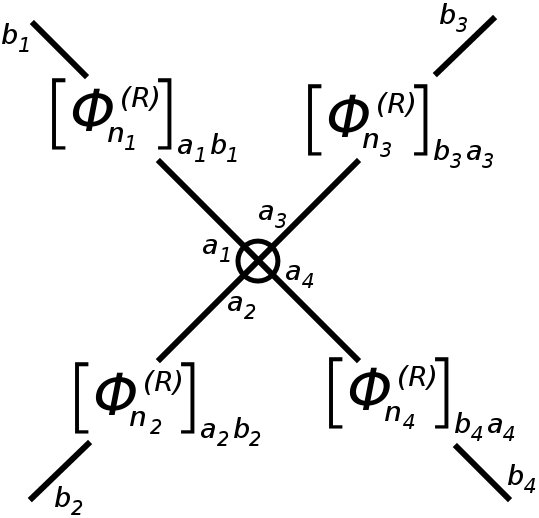
\includegraphics[width=0.30\textwidth]{plots/SFdefdiag.png}
  \end{center}
  \caption{
  Representation of the amplitude involving four Wilson lines.
  }
  \label{fig:SFamp}
\end{figure}

The operator $\mathbold{O}_s$ is defined as a product of Wilson lines, which
mediate soft gluon exchanges between particles and give rise to colour
correlations.
% 
The Wilson line for a particle in representation $R$, moving along the straight
line with $d$-momentum $n_i$ between the points $x+a n_i$ and $x+b n_i$, is
defined as~\cite{Czakon:2013hxa}
%
\begin{equation}
  \left[\mathbold{\Phi}_{n_i}^{(R)} (x; b, a)\right]_{a_i b_i} =
  \left\{
  \calP 
  \exp 
  \left( i g_s^0 \int_a^b\!\! dt\, n_i \cdot 
  A^c(x+t\, n_i)\, \cT^{(R)\, c}
  \right)
  \right\}_{a_i b_i}
  \,,
  %\label{eq:}
\end{equation}
%
where $\calP$ denotes path ordering. The indices $a_i$ and $b_i$ arise since the
Wilson line is an operator in colour space and it accounts for colour evolution
of a particle due to gluon emissions.
%
The operator $\mathbold{O}_s$ for top quark pair production in the
\qqbar channel is given by
%
\begin{equation}
  \mathbold{O}_s(x) = 
  \left[\mathbold{\Phi}_{v_3}^{(3)} (x; \infty, 0)\right]_{b_3 a_3} 
  \left[\mathbold{\Phi}_{v_4}^{(\bar 3)} (x; \infty, 0)\right]_{b_4 a_4} 
  \left[\mathbold{\Phi}_{n}^{(3)} (x; 0, -\infty)\right]_{a_1 b_1} 
  \left[\mathbold{\Phi}_{\bar n}^{(\bar 3)} (x; 0, -\infty)\right]_{a_2 b_2} \,,
  \label{eq:Osqqdef}
\end{equation}
%
and in the $gg$ channel
%
\begin{equation}
  \mathbold{O}_s(x) = 
  \left[\mathbold{\Phi}_{v_3}^{(3)} (x; \infty, 0)\right]_{b_3 a_3} 
  \left[\mathbold{\Phi}_{v_4}^{(\bar 3)} (x; \infty, 0)\right]_{b_4 a_4} 
  \left[\mathbold{\Phi}_{n}^{(8)} (x; 0, -\infty)\right]_{a_1 b_1} 
  \left[\mathbold{\Phi}_{\bar n}^{(8)} (x; 0, -\infty)\right]_{a_2 b_2} \,.
  \label{eq:Osggdef}
\end{equation}

%-----------------------------------------------------------------------------
\subsection{Azimuthal averaging}

As we see in Eq.~(\ref{eq:factorization-scet}), the factorization formula
involves integration over $\phi$, the azimuthal angle between $x_\perp$ an
$v_3$. If we restrict ourselves to the NNLO cross section for top quark pair
production, the NNLO soft function will enter the factorization
formula~(\ref{eq:factorization-scet}) multiplied by the leading order hard
function and the leading order beam functions, both of which are Lorentz
scalars.  Hence, the integration over the azimuthal angle can be pulled directly
to the soft function. This motivates us to define the averaged soft function
%
\begin{equation}
  \bfS_{i\bar i}(x_\perp) = 
  \int \frac{d\Omega_{d-3}}{S_{d-3}} \bm{W}_{i\bar i}(x_\perp)\,,
  \label{eq:sf-avd}
\end{equation}
%
with $d\Omega_{d-3}$ being a rotationally-invariant measure on the unit
$(d-3)$-sphere, defined recursively as
%
\begin{equation}
  \int_{S_1^{d-3}}\!\!\! d\Omega_{d-3} =
  \int_{S_1^{d-3}}\!\!\! d\Omega(\theta_1,\theta_2,\ldots,\theta_{d-3}) =
  \int_0^\pi\!\! d\theta_1 \sin^{d-4}\theta_1
  \int_{S_1^{d-4}}\!\!\! d\Omega(\theta_2,\ldots,\theta_{d-3})\,,
  \label{eq:rot-inv-measure}
\end{equation}
%
with
%
\begin{equation}
  \theta_1,\ldots,\theta_{d-4} \in [0,\pi]\,,\qquad \qquad
  \theta_{d-3} \in [0,2\pi]\,,
  %\label{eq:}
\end{equation}
%
while $S_{d-3}$ is this sphere's surface, which can be calculated from the
general formula
%
\begin{equation}
  S_{d}= \frac{2\pi^{(d+1)/2}}{\Gamma[(d+1)/2]}\,.
  \label{eq:Sd}
\end{equation}
%
We note that the averaging of Eq.~(\ref{eq:sf-avd}) is defined in $d-3$
dimensions as the entire calculation of the NNLO soft function is performed
consistently in $d$ dimensions.  That implies that all external and internal
momenta, as well as polarizations, are $d$-dimensional.

The averaged soft function can be expanded as perturbation series 
\begin{equation}
  \bfS_{i\bar i}(x_\perp) = 
  \sum_{n=0}^\infty \bfS_{i\bar i}^{(n)}(x_\perp) \left(\asp\right)^n\,.
  \label{eq:sf-expansion}
\end{equation}

Finally, we mention that in order to compute the complete NNLO cross section for
\ttbar production in the $gg$ channel, one also needs a version of the NLO soft
function which is averaged azimuthally together with the $x_\perp^\mu
x_\perp^\nu$ Lorentz structure which comes from the NLO gluon beam
function~\cite{Gehrmann:2014yya}.
%
This component can be obtained using the unaveraged NLO soft function of
Ref.~\cite{Catani:2014qha}.


%----------------------------------------------------------------------------
\subsection{Colour space}

The soft function discussed so far is an abstract operator in colour space. It
turns out to be useful to represent it as a matrix, with the elements 
%
\begin{equation}
 S_{IJ} = \langle c_I | \bfS | c_J \rangle\,.
  %\label{eq:}
\end{equation}
%
We choose the basis vectors, $|c_I\rangle = \big(c_I^{i\bar i}\big)_{\{a\}}$,
following Ref.~\cite{Ferroglia:2012uy}.
%
In the $q\qbar$ channel, they read
%
% NOTE
%
% ttbar/complete/2cut/soft-function-all-orders.nb
%
\begin{equation}
  %\label{eq:}
  \left(c_1^{q\bar{q}}\right)_{\{a\}} = \delta_{a_1a_2} \,\delta_{a_3a_4}\,,
  \qquad
  \left(c_2^{q\bar{q}}\right)_{\{a\}} = t_{a_2a_1}^c \, t_{a_3a_4}^c\,,
  \label{eq:colour-basis-qq}
\end{equation}
%
and in the $gg$ channel
%
\begin{equation}
    \left(c_1^{gg}\right)_{\{a\}} = \delta^{a_1a_2} \, \delta_{a_3a_4} \, , 
    \qquad
    \left(c_2^{gg}\right)_{\{a\}} = i f^{a_1a_2c} \, t^{c}_{a_3a_4} \, , 
    \qquad
    \left(c_3^{gg}\right)_{\{a\}} = d^{a_1 a_2 c} \, t^c_{a_3a_4} \, .
  \label{eq:colour-basis-gg}
\end{equation}
%
The inner product is defined as a sum over all colour indices
%
\begin{equation}
  \langle c_I | c_J \rangle = 
  \sum_{\{a\}} 
  \left( c_I \right)^*_{a_1 a_2 a_3 a_4}
  \left( c_J \right)_{a_1 a_2 a_3 a_4}\,.
  %\label{eq:}
\end{equation}
%
The above basis vectors are orthogonal but not
orthonormal~\cite{Ferroglia:2012uy}.

The NLO and NNLO contributions to the soft function can be represented as
%
\begin{eqnarray}
  \bfS^{(1)}_\text{bare}(x_\perp) & = &
  \sum_{i,j} \mathbold{w}_{ij}^{(1)}\, I_{ij}(\xT)\,, 
  \label{S1bareNLO}
  \\
  %
  \bfS^{(2)}_\text{bare}(x_\perp) & = &
  \sum_{i,j} \mathbold{w}^{(1)}_{ij}\, I_{ij}^{(1)}(\xT) +
  \sum_{i,j,k,l} \mathbold{w}^{(2S)}_{ijkl}\, I_{ijkl}^{(2)}(\xT) +
  \sum_{i,j,k} \mathbold{w}^{(2A)}_{ijk}\, I_{ijk}^{(2)}(\xT)\,,
  \label{S1bareNNLO}
\end{eqnarray}
%
where $\mathbold{w}$ are the colour matrices defined as
% NOTE
%
% calculated in ttbar/secdec/double-emission-tensor/input-list.nb
%
\begin{subequations}
  \begin{align}
   \bm{w}_{ij}^{(1)} & =
   \frac{1}{d_R} \langle c_I | \cT_i\cdot\cT_j | c_J \rangle\,,
   \label{eq:w1def}
   \\[0.5em]
   \bm{w}_{ijkl}^{(2S)} & =
   \frac{1}{d_R} \langle c_I | \left\{\cT_i\cdot\cT_j, \cT_k\cdot\cT_l\right\} 
   | c_J \rangle\,,
   \label{eq:w2def}
   \\[0.5em]
   \bm{w}_{ijk}^{(2A)} & =
   \frac{1}{d_R} \langle c_I | \left[\cT_i\cdot\cT_k, \cT_j\cdot\cT_k\right] 
   | c_J \rangle\,.
   \label{eq:w3def}
  \end{align}
  \label{eq:w1w2def}
\end{subequations}
%
The Hermitian, colour operators $\cT_i$ satisfy the following
relations~\cite{Catani:1996vz}
%
\begin{equation}
\cT_i \cdot \cT_j=\cT_j\cdot\cT_i = T^c_iT^c_j, \quad
\cT_i \cdot \cT_i\,  = \cT_i^2=C_i\, \unitop =C_{a_i}\, \unitop, \quad
\sum_{i}\cT_i|\cm_{n}\ra=0 \,,
\end{equation}
%
where $\unitop$ is the identity operator, $a_i \in \{q, \qbar, g\}$, and
$C_g = C_A,\, C_q = C_{\bar{q}} = C_F$.
The operators $\cT_i$ act on vectors in the colour space as follows
%
\begin{eqnarray}
\la c_1,\dots,c_i,\dots,c_n,c|\cT_i|b_1,\dots,b_i,\dots,b_n\ra &=&
\la c_1,\dots,c_i,\dots,c_n|T^c_i|b_1,\dots,b_i,\dots,b_n\ra
\nonumber\\ &=& \delta_{c_1b_1} \dots T^c_{c_i b_i}\dots\delta_{c_nb_n} \; .
\end{eqnarray}
%
The matrix elements of the $i^\text{th}$ parton operator, $\cT_i$, are given by
$\left(\cT^c_i\right)_{c_1c_2} = if^{c_1cc_2}$, for an initial-state and
final-state gluon, $\left(\cT^c_i\right)_{c_1 c_2}= t^c_{c_1 c_2} (= -t^c_{c_2
c_1})$, for a final-state quark (anti-quark), and $\left(\cT^c_i\right)_{c_1 c_2} =
-t^c_{c_2 c_1} (= t^c_{c_1 c_2})$, for an initial-state quark (anti-quark).



%-----------------------------------------------------------------------------
\subsection{Fourier transform}

In practice, it is easier to calculate the soft function in momentum space. The
relevant scalar integrals, which appear in Eqs.~(\ref{S1bareNLO}) and
(\ref{S1bareNNLO}), can be transferred to momentum space by means of the Fourier
transform 
%
\begin{subequations}
   \begin{eqnarray}
     \label{eq:fourier-transformd}
     \tilde I_{\{i\}} (q_\perp)& = &
     \frac{1}{\left(2\pi\right)^{\frac{d-2}{2}}}
     \int d^{d-2} x_\perp I_{\{i\}} (x_\perp) \, e^{i x_\perp \cdot q_\perp}\,,
     \\
     \label{eq:fourier-transform-inv}
     I_{\{i\}} (x_\perp)& = &
     \frac{1}{\left(2\pi\right)^{\frac{d-2}{2}}}
     \int d^{d-2} q_\perp \tilde I_{\{i\}} (q_\perp) \, e^{-i x_\perp \cdot
     q_\perp}\,,
   \end{eqnarray}
\end{subequations}
%
where $\{i\}$ represents the two, three or four particle indices.
%
The structure of the $I_{\{i\}}(x_\perp)$ integrals, for all types of diagrams
encountered at NNLO, is
%
\begin{equation}
  I_{\{i\}}(x_\perp) = 
\int d^d p
  \, e^{-i x_\perp \cdot p_\perp}\,
  \times (...)\,,
  \label{eq:Igenform}
\end{equation}
%
where the ellipsis depend on details of the graph, \ie the direction of the
Wilson lines and the soft parton emissions, and $p$ denotes the total momentum
of the latter.

By plugging Eq.~(\ref{eq:Igenform}) to Eq.(\ref{eq:fourier-transformd}), we
obtain
%
\begin{align}
  \tilde I_{\{i\}}(q_\perp)  & = 
 (2\pi)^{\frac d2-1}
\int d^d p
 \,  
  \delta^{(d-2)}(p_\perp-q_\perp)
  \times (\dots) \,. \label{eq:defmspace}
\end{align}
%
And by applying the azimuthal averaging of Eq.~(\ref{eq:sf-avd}) we get
%
\begin{align}
\int \frac{d\Omega_{d-3}}{ S_{d-3}}\,  \tilde I_{\{i\}}(q_\perp) 
  & =
  \frac{(2\pi)^{\frac d2-1}}{ S_{d-3}}
  \int d^{d}p\,  d\Omega_{d-3}\,
  \delta^{(d-2)}(p_\perp-q_\perp)
  \times (\dots) 
  \label{eq:avmagic1}
  \\
  & = 
  \frac{(2\pi)^{\frac d2-1}}{ S_{d-3}}
  \int \frac{d^dp}{q_T^{d-3}}\, \delta(p_T-q_T)
  \times (\dots) \,.
  \label{eq:avmagic2}
\end{align}
%
In the above, we used rotational invariance of the measures and the fact that
the order of the integrations can be changed. This leads to a reinterpretation of the
angles in $d\Omega_{d-3}$ as the azimuthal angles of $q_\perp$ and that allows
one to go from (\ref{eq:avmagic1})  to (\ref{eq:avmagic2}) with the help of the
identity
%
\begin{equation}
  \int d\Omega_{d-3}\, \delta^{(d-2)} (p_\perp-q_\perp) =
  \frac{1}{q_T^{d-3}}\, \delta(p_T-q_T)\,.
  %\label{eq:}
\end{equation}
%
Now, we rescale the momenta associated to the emissions by $q_T$, in particular $\tilde{p}^\mu=q_T p^\mu$ , and get
%
\begin{align}
\int \frac{d\Omega_{d-3}}{ S_{d-3}}\,  \tilde I_{\{i\}}(q_T) 
  & = 
  \frac{1}{q_T^r}
  \frac{\left(2\pi\right)^{\frac{d}{2}-1}}{ S_{d-3}}
  \int d^d\tilde p\, \delta(\tilde p_T-1)
  \times (\dots) \,.
\end{align}
%
Above, the overall power of $q_T$ has been denoted as $r$. It is a sum of the
contribution from the $d-2$-dimensional delta function and a genuine
contribution from the graph part.
%
The rescaling factorizes all the $q_T$ dependence. As a consequence, all
integrals in momentum space are proportional to the factor $1/q_T^r$, with the
power $r$, which depends on the order of perturbative expansion. Hence, the
transformation from momentum to position space, by means of the Fourier
Transform~(FT), will amount to multiplication by a factor given by the compact
expression 
%
% NOTE 
% - my folder notes
% - ttbar/vp-terms/CalculateFourierTransform.m
% - ttbar/vp-terms/CheckFourierTransform.nb
%
\begin{align}
  \text{FT}\left[\frac{1}{q_T^r}\right]^{d-2} 
   & =
   2^{-2 + 3\epsilon + r}
   \sqrt{\pi}\,
   \left(\frac{e^{-\gamma_E+\frac12\LT}}{\mu}\right)^{-2+2\epsilon+r}
   \!\!\!\!\!\!
   \frac{\Gamma(2-2\epsilon-r)}{
   \Gamma\left(\frac{3}{2}- \epsilon -\frac{r}{2}\right)
   \Gamma\left(\frac{r}{2}\right)}.
   \label{eq:FTfinal}
\end{align}
% 
At NLO, $r=2+\alpha$, and at NNLO, $r=2+2\alpha+2\epsilon$ for double-cut
diagrams and $r=2+\alpha+2\epsilon$, for single-cut diagrams, where $\alpha$ is
the analytic regulator discussed in the next section. An important feature of
(\ref{eq:FTfinal}), both at NLO and NNLO, is that its expansion begins at
order $1/\epsilon$ 
%
\begin{equation}
  \text{FT}\left[\frac{1}{q_T^{2+\alpha}}\right]^{d-2}  = 
  -\frac{1}{2\epsilon} + \order{\alpha/\epsilon^2}\,,
  \qquad
  \text{FT}\left[\frac{1}{q_T^{2+2\alpha+2\epsilon}}\right]^{d-2}   =
  -\frac{1}{4\epsilon} + \order{\alpha/\epsilon^2}\,.
  \label{eq:FTexpand}
\end{equation}
%
Hence, to obtain a result in position space at the order
$\epsilon^0$, one needs to calculate the momentum-space soft function up to
$\epsilon^1$.


%-----------------------------------------------------------------------------
\subsection{Analytic regulator}

The phase space integrals $\tilde I_{\{i\}}$ turn out to be divergent not only
when the gluons become soft, but also in the limit where the light-cone
components of gluons' momenta tend to zero or infinity. Through the relation
%
\begin{equation}
  y_g = \frac12 \ln \frac{k_+}{k_-}\,,
  %\label{eq:}
\end{equation}
%
this limit occurs when the gluon rapidity $y_g \to \pm \infty$. That is why,
these are called ``rapidity divergencies''. They arise because, in SCET, we
approximate the full QCD Feynman integrals following the expansion by regions.
Yet, we integrate each expression over the full phase space of gluons' momenta.
We note that this does not give rise to double counting~\cite{Becher:2014oda}.
Nevertheless, it forces us to introduce another regulator to handle the
integrals.

The reason why contributions from different regions do not overlap even when
integrated from $-\infty$ to $+\infty$ is that integrals in each region depend
on a single scale and expanding them further (\eg soft integrals in the
collinear region) leads to scaleless integrals, which vanish.

In our calculation, we chose to adopt the analytic regulator prescription of
Ref.~\cite{Becher:2011dz}, which amounts to the following replacement of the
integration measure
%
\begin{equation}
 \int d^d k\, \delta^{+}(k^2)  \to
 \int d^d k \left(\frac{\nu}{n\cdot k}\right)^\alpha \delta^{+}(k^2)\,,
  %\label{eq:}
\end{equation}
%
where $\nu$ is a free parameter introduced for dimensional reasons (an analogue
of $\mu$ in dimensional regularization) and we denote $\delta^+(k^2) =
\delta(k^2) \theta(k_0)$.
%
The regulator $\alpha$ becomes necessary at intermediate stages of the
calculation. Since rapidity divergencies do not appear in full QCD, the result
for the complete cross section is finite in the limit $\alpha \to 0$.
%
In the case of the analytic regulator, the poles in $\alpha$ cancel not only at
the level of the cross section but even at the level of the soft function. This
comes from the fact that the soft function for the Drell-Yan process is equal to
one, which implies that the product of the beam functions is
$\alpha$-independent (but not the beam functions themselves, see
Ref.~\cite{Gehrmann:2014yya}). As beam functions are universal, the same,
$\alpha$-independent product of the beam functions is used in the process of
\ttbar production. This means that the only dependence on $\alpha$ can occur in
the soft function. Therefore, all $\alpha$ poles have to vanish within the 
latter. We shall use this feature as one of validations of our calculation.

%-----------------------------------------------------------------------------
\subsection{Renormalization}
\label{sec:renormalization}

%-----------------------------------------------------------------------------
The renormalized soft function of the small-$q_T$ factorization satisfies the
following renormalization group evolution~(RGE) equation~\cite{Zhu:2012ts}
%
% NOTE
% also my paper notes in the folder
%
\begin{equation}
  \frac{d}{d\ln \mu} \bfS_\iibar (\mu) =
  - \bfgamma^{s \dagger}_\iibar \,\bfS_\iibar (\mu)  
  - \bfS_\iibar (\mu)\, \bfgamma^{s}_\iibar \,,
  \label{eq:SF-RGE-main}
\end{equation}
%
where
%
\begin{equation}
  \bfgamma^{s}_\iibar = \bfgamma^{h}_\iibar - 2 \gamma^{i} \bfI\,,
  %\label{eq:}
\end{equation}
%
and $\bfgamma^{h}_\iibar$ is defined as a non-$\Gamma_\text{cusp}$ part of the
full anomalous dimension matrix $\bfGamma$~\cite{Ahrens:2010zv}, while
$\gamma^{i}$ is the massless-particle anomalous dimension (and enters RGE
equations for beam functions in Drell-Yan and Higgs
production~\cite{Becher:2010tm, Becher:2012yn}). To make the notation lighter
we shall omit the index $\iibar$, keeping in mind that the soft
function and the anomalous dimension are different in the \qqbar and $gg$
channels.

The soft anomalous dimension matrix $\bfgamma^{s}$ is related to the soft
renormalization factor (also a matrix in colour space), $\bfZ_s$, as follows
%
\begin{equation}
  \bfgamma^{s} = - \bfZ_s^{-1}\frac{d\bfZ_s}{d\ln \mu}\,,
  \label{eq:softAD}
\end{equation}
%
and $\bfZ_s$ absorbs all UV divergences such that
%
\begin{equation}
  \bfS(\mu) = \bfZ^\dagger_s(\mu,\epsilon) \bfS_\bare(\epsilon)
  \bfZ_s(\mu,\epsilon)\,.
  %\label{eq:}
\end{equation}
%
Each quantity in the above equation has a perturbative expansion, either in the
renormalized coupling, 
$a_s = \alpha_s/(4\pi)$, 
or in the bare coupling,
$a_s^0 = \alpha_s^0/(4\pi)$, 
and the relation between the two is
%
\begin{equation}
  a_s^0(\epsilon) = 
  \left(\frac{\mu^2 e^{\gamma_E}}{4\pi}\right)^\epsilon Z_\alpha a_s
  \equiv \xi_\as(\epsilon,\mu)\, Z_\alpha\, a_s (\mu)\,,
  \label{eq:alpha}
\end{equation}
%
where the \msbar renormalization constant reads
%
\begin{equation}
  Z_\alpha = 
  1- \frac{\beta_0 \as}{4\pi \epsilon} + \ldots =
  1- \frac{\beta_0}{\epsilon} a_s(\mu) + \ldots\,,
  \label{eq:Zalpha}
\end{equation}
%
and $\beta_0$ is the one-loop coefficient of the QCD $\beta$ function
given in Eq.~(\ref{eq:beta0def}).
%
Hence, substitution of Eq.~(\ref{eq:sf-expansion}) for the bare and renormalized
soft function, as well as Eqs.~(\ref{eq:alpha}) and~(\ref{eq:Zalpha}) to
Eq.~(\ref{eq:SF-RGE-main}) leads to the following, order-by-order relations
%
\begin{eqnarray}
  \bfS^{(0)} & = &  \bfS^{(0)}_\bare \,,
  \\[0.5em]
  \bfS^{(1)} & = &
  \bfZ^{\dagger (1)}_s \bfS^{(0)}_\bare  + \bfS^{(0)}_\bare \bfZ^{(1)}_s  +
  \xi_\as \bfS^{(1)}_\bare \,,
  \\[0.5em]
  \bfS^{(2)} & = &
  \bfZ^{\dagger (2)}_s \bfS^{(0)}_\bare  + \bfS^{(0)}_\bare \bfZ^{(2)}_s  +
  \bfZ^{\dagger (1)}_s \bfS^{(0)}_\bare \bfZ^{(1)}_s 
  \nonumber \\[0.5em]
  & &
  + \bfZ^{\dagger (1)}_s \xi_\as \bfS^{(1)}_\bare  + 
  \xi_\as \bfS^{(1)}_\bare \bfZ^{(1)}_s  +
  \xi_\as^2 \bfS^{(2)}_\bare 
  -\frac{\beta_0}{\epsilon}\, \xi_\as \bfS^{(1)}_\bare
  \,.
  \label{eq:S2ren}
\end{eqnarray}
%
The quantities on the l.h.s. are finite in the limit $\epsilon \to 0$. The
$\bfZ^{(i)}_s$ factors have only singular terms with poles in $\epsilon$, while
the bare functions, $\bfS^{(1)}_\bare$ and $\bfS^{(2)}_\bare$, have both
singular and finite parts.

For notational simplicity, in what follows we will absorb the $\xi_\as$
prefactors into the definitions of the bare soft functions and change the
notation according to
%
\begin{equation}
  \xi_\as^n \bfS^{(n)}_\bare \to
  \bfS^{(n)}_\bare\,.
  %\label{eq:}
\end{equation}
%

At the order $a_s^2$, from Eq.~(\ref{eq:S2ren}), we get
%
\begin{eqnarray}
  \underbrace{\bfS^{(2)}}_{\text{finite part only}}   
  &  =  &
  \overbrace{\bfZ^{\dagger (2)}_s \bfS^{(0)}_\bare  + 
   \bfS^{(0)}_\bare \bfZ^{(2)}_s  +
   \bfZ^{\dagger (1)}_s \bfS^{(0)}_\bare \bfZ^{(1)}_s}^{\text{(I) pole part only}} 
  \nonumber \\
  & &
  \quad +  \quad 
  \underbrace{\bfZ^{\dagger (1)}_s \bfS^{(1)}_\bare  + 
  \bfS^{(1)}_\bare \bfZ^{(1)}_s  +
  \bfS^{(2)}_\bare
 -\frac{\beta_0}{\epsilon}\, \bfS^{(1)}_\bare
  }_{\text{(II) finite + pole part}} \,.
  \label{eq:renS2}
\end{eqnarray}
%
Part (I) on the r.h.s. has only terms singular in $\epsilon$, which come
from the fact that the $\bfZ_s$ factors are defined in the \msbar scheme. 

These pole terms have to cancel against the singular terms of part (II),
which can be used in the following way:
%
knowing $\bfZ_s^{(1)}$ and $\bfZ_s^{(2)}$, as well as $\bfS^{(0)}_\bare$ and
$\bfS^{(1)}_\bare$, allows one to cross-check all the singular terms of
the $\bfS^{(2)}_\bare$ function obtained from direct calculation.
%
The explicit form of the $\bfZ_s$ factor, together with the relevant anomalous
dimensions are given in Appendix~\ref{app:AD}.

%-----------------------------------------------------------------------------
\subsection[Determination of $L_\perp$-dependent terms of the soft
function from RGE]{Determination of $\mathbold{L_\perp}$-dependent terms of the soft function from RGE}

\label{sec:RGevolution}


The RGE equation (\ref{eq:SF-RGE-main}) can be written as
%
\begin{equation}
  \frac{d}{d L_\perp} \bfS(\mu) =
  - \frac{1}{2} \left[
  \bfgamma^{s \dagger}\,\bfS(\mu)  
  + \bfS(\mu)\, \bfgamma^{s}
  \right]\,,
  \label{eq:SF-RGE-Lp}
\end{equation}
%
where $\LT$ was defined in Eq.~(\ref{eq:LTdef}).
%
Both the soft function and the anomalous dimension have perturbative expansions
%
\begin{eqnarray}
  \bfS  & = &
  \bfS^{(0)} + a_s \bfS^{(1)} + a_s^2 \bfS^{(2)} + \ldots\,,
  \label{eq:Sren-exp}
  \\
  \bfgamma_{s} & = &
  a_s \left(\bfgamma_{s,0} + a_s \bfgamma_{s,1}+ \ldots\right)\,.
  \label{eq:gammas-exp}
\end{eqnarray}
%
All quantities in the above equations are renormalized and they are defined in
$d$ dimensions.
 
Because the anomalous dimension matrix starts at the order $a_s$,
Eq.~(\ref{eq:SF-RGE-Lp}) can be solved iteratively. We just need to plug
Eqs.~(\ref{eq:Sren-exp}) and (\ref{eq:gammas-exp}) into 
Eq.~(\ref{eq:SF-RGE-Lp}) and  remember that the renormalized, 4-dimensional
coupling $a_s$ also depends on $\ln\mu$, which implies
%
\begin{equation}
  \frac{d a_s}{dL_\perp} = \frac12 \frac{d a_s}{d\ln\mu} = 
  \frac12 \frac{\partial a_s}{\partial \ln\mu} = 
  \frac12 \frac{\beta(a_s)}{4\pi} = 
  - \beta_0\, a_s^2 + \order{a_s^3}\,,
  %\label{eq:}
\end{equation}
%
where we used the expansion of the QCD $\beta$ function given in
Eq.~(\ref{eq:betaexp}).

After collecting terms at each order, we
arrive at the following differential equations
%
\begin{eqnarray}
  \frac{d}{dL_\perp} \bfS^{(0)} & = &  0\,,
  \\
  \frac{d}{dL_\perp} \bfS^{(1)} & = & 
  -\frac12\left[
  \bfS^{(0)}\, \bfgamma_{s,0} + \bfgamma_{s,0}^\dagger\, \bfS^{(0)} 
  \right]\,,
  \\
  \frac{d}{dL_\perp} \bfS^{(2)} & = & 
  -\frac12\left[
  \bfS^{(1)}\, \bfgamma_{s,0} + \bfgamma_{s,0}^\dagger\, \bfS^{(1)}  
  - 2 \beta_0 \bfS^{(1)}  +
  \bfS^{(0)}\, \bfgamma_{s,1} + \bfgamma_{s,1}^\dagger\, \bfS^{(0)} 
  \right]\,.
  %\label{eq:}
\end{eqnarray}
 
Hence, knowing the soft anomalous dimension to order $a_s^2$, and the soft
function to order~$a_s^1$ allows one to determine all pieces of the soft
function at order $a_s^2$ except the constant, \ie $\LT$-independent term.
Specifically, at order $a_s^2$, we get
%
% NOTE
% my folder notes
%
\begin{eqnarray}
  \bfS^{(2)} 
  & = & 
  -\frac12\Bigg\{
  \frac12\left[
  \bfS^{(1)}_{L_\perp}\, \bfgamma_{s,0} + 
  \bfgamma_{s,0}^\dagger\, \bfS^{(1)}_{L_\perp}  
  - 2 \beta_0 \bfS^{(1)}_{L_\perp} 
  \right] L_\perp^2
   \\
  & &
  \hspace{25pt} + \left[
  \bfS^{(1)}_{\slashed{L}_\perp}\, \bfgamma_{s,0} + 
  \bfgamma_{s,0}^\dagger\, \bfS^{(1)}_{\slashed{L}_\perp}  
  - 2 \beta_0 \bfS^{(1)}_{\slashed{L}_\perp} +
  \bfS^{(0)}\, \bfgamma_{s,1} + \bfgamma_{s,1}^\dagger\, \bfS^{(0)} 
  \right] L_\perp
  \Bigg\} 
  + \text{const}\,,
  \nonumber
\end{eqnarray}
%
where $\bfS^{(1)}_{L_\perp}$ and $\bfS^{(1)}_{\slashed{L}_\perp}$ denote,
respectively, the $L_\perp$-dependent and $L_\perp$-independent pieces of the
$\bfS^{(1)}$ soft function.



%-----------------------------------------------------------------------------
\section{NLO soft function}
\label{sec:NLOsf}

The leading order soft function corresponds to the case without radiation. It is
given by the following, constant matrices~\cite{Li:2013mia, Ferroglia:2012uy}
%
\begin{equation}
 \bfS^{(0)}_{q\qbar}  =  
 \left( \begin{array}{cc}
   N & 0 \\
   0 & \frac{C_F}{2} 
 \end{array} \right)\,,
 \qquad
 \bfS^{(0)}_{gg}  =  
 \left( \begin{array}{ccc}
   N & 0           & 0 \\
   0 & \frac{N}{2} & 0 \\
   0 & 0           & \frac{N^2-4}{2N}
 \end{array} \right)\,,
\end{equation}
%
respectively for the $\qqbar$ and $gg$ channels.
%
Because the LO soft function is not divergent, the above result corresponds both to the bare and the renormalized case. Hence, we see that  $\bfZ_{i\bar
i}^{(0)} =  \idop$.

The next-to-leading order, bare soft function, is given by
%
\begin{equation}
  \bfS_{i\bar i}^{(1), \bare} = 
  \sum_{i,j = 1,\ldots,4} \!\!\! \bm{w}_{ij}^{(1)} I_{ij}\,,
  \label{eq:S-W-Iij}
\end{equation}
%
where the colour structure is encoded in the $\bm{w}_{ij}^{(1)}$
matrices defined as
%
\begin{equation}
  \Big(\bm{w}_{ij}^{(1)}\Big)_{IJ} =
  \frac{1}{d_R} \langle c_I |\bm{T}_i \cdot \bm{T}_j | c_J \rangle\,,
  \label{eq:w1matrixdef}
\end{equation}
%
with the basis vectors $| c_J \rangle$ introduced in
Eqs.~(\ref{eq:colour-basis-qq}) and~(\ref{eq:colour-basis-gg}).
%
For the sake of notational simplicity, in what follows, we suppress the index
$\iibar$ in the colour matrices. It can always be inferred either from the
context, or based on the size  of a matrix.
The explicit expressions for colour matrices (\ref{eq:w1matrixdef}) are given in
Appendix~\ref{app:colmat}.


\begin{figure}[t]
  \begin{center}
    \hspace{40pt}
    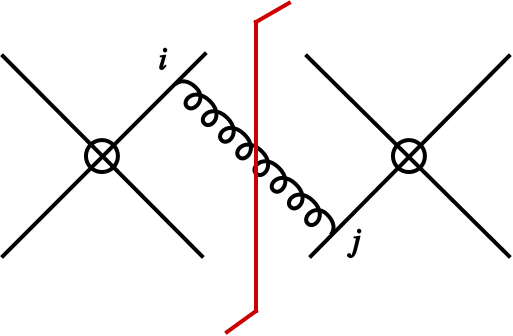
\includegraphics[width=0.30\textwidth]{plots/sf-nlo.png}
  \end{center}
  \caption{Feynman diagram for the NLO soft function.  The solid lines pointing
  towards the cut represent the Wilson lines of the top quarks. The lines
  pointing away from the cut correspond to the Wilson lines of the incoming,
  massless partons, quarks or gluons. The diagram represents a class of graphs
  with all possible gluon connections between the Wilson lines.
  }
  \label{fig:sf-nlo}
\end{figure}

$I_{ij}$s in Eq.~(\ref{eq:S-W-Iij}) correspond to phase-space integrals,
represented diagrammatically in Fig.~\ref{fig:sf-nlo}.
The solid lines pointing towards the cut represent the 
top quarks. The lines pointing away from the cut correspond to the
incoming, massless partons.
%
The momentum-space versions of the integrals represented in
Fig.~\ref{fig:sf-nlo}, obtained with the Fourier
transform~(\ref{eq:fourier-transformd}), read
%
\begin{equation}
  \tilde I_{ij} =  
  (4\pi)^2  \left(\frac{\mu^2 e^{\gamma_E}}{4\pi}\right)^\epsilon 
    \frac{(2\pi)^{\frac{d}{2}-1}}{ S_{d-3}\, q_T^{d-3}} 
  \int \frac{d^d k}{(2\pi)^{d-1}}
  \left(\frac{\nu}{n\cdot k}\right)^\alpha
  \delta(k^2)\, \theta(k^0)\,
  \delta(k_T - q_T)
  \frac{(-v_i \cdot v_j)}{v_i \cdot k\; v_j \cdot k}\,,
  \label{eq:soft-func-nlo-mom-space-ddim}
\end{equation}
%
where $\left(\frac{\mu^2 e^{\gamma_E}}{4\pi}\right)^\epsilon$ comes from
renormalization of the strong coupling, see Eq.~(\ref{eq:alpha}), and the remaining
prefactors arise from the Fourier transform and azimuthal averaging.
%
Only the real-type diagrams contribute to the NLO soft function as the virtual
graphs are scaleless and vanish.

The integration measure can be written as $d^d k = d k_+ d k_- d^{d-2} k_\perp$
and the $k_+$ and $k_-$ components are integrated from minus to plus infinity.
However, the phase space of integration of these light-cone momenta is
restricted by $\delta(k^2)\, \theta(k^0)$ appearing in
Eq.~(\ref{eq:soft-func-nlo-mom-space-ddim}).  This can be easily seen by
rewriting the above condition as $\delta(k_+ k_- - k_T^2)\, \theta(k_+ + k_-)$.
The delta function fixes $k_+ k_- = k_T^2 > 0$, hence the light-cone components
must be both positive or negative.  And the theta function, chooses them to be
both positive. All in all, the integration over $d k_+ d k_-$ is restricted to
the line depicted in Fig.~\ref{fig:light-cone-phase-space} (left).

The NLO soft function has been calculated up to order $\epsilon^0$ in
Refs.~\cite{Li:2013mia, Catani:2014qha}. However, as can be seen from
Eq.~(\ref{eq:renS2}), to renormalize the NNLO soft function, we need to
know the NLO soft function up to the order $\epsilon^1$. This order has been
calculated in Ref.~\cite{AntoniaMTh}, yet, using a slightly different definition
of azimuthal averaging. We have adjusted this result to our definition, as well
as fully cross checked it using a sector decomposition-based approach (described
in detail in Section~\ref{sec:secdec}), finding a perfect agreement.

\begin{figure}[t]
  \begin{center}
    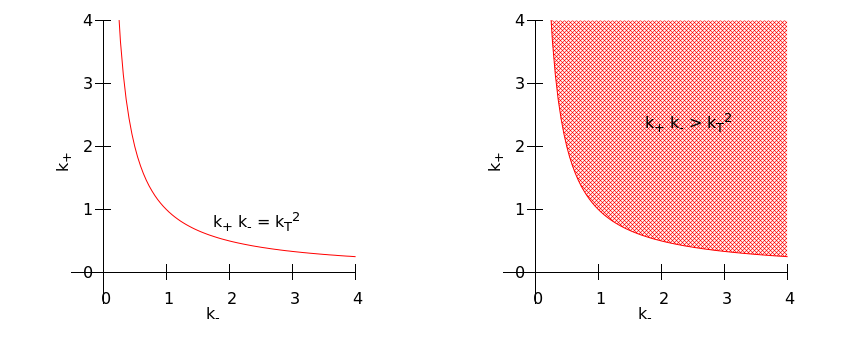
\includegraphics[width=0.99\textwidth]{plots/light-cone-phase-space.png}
  \end{center}
  \caption{
  Integration regions over the light-cone components of the on-shell (left) and
  off-shell gluon. The former corresponds to the integrals of the NLO soft
  function defined in Section~\ref{sec:NLOsf}, the latter to bubble integrals of
  the NNLO soft function discussed in Section~\ref{sec:debubble}.
  }
  \label{fig:light-cone-phase-space}
\end{figure}


Hence, the final result for the position-space NLO soft function up to order
$\epsilon^1$ reads
%
% NOTE
% ttbar/complete/1cut/nlo/s1-analytic.nb
%
\allowdisplaybreaks
\begin{align}
\bfS_{i\bar i}^{(1)}  & =  
-4\, \bfw_{13}^{(1)}
\left[\text{Li}_2\left(1-\frac{t_1 u_1}{m_t^2 M^2}\right)
-2 L_\perp \ln \frac{-t_1}{m_t M}\right]
%
-4\, \bfw_{23}^{(1)}
\left[\text{Li}_2\left(1-\frac{t_1 u_1}{m_t^2 M^2}\right)
-2 L_\perp \ln \frac{-u_1}{m_t M}\right]
%
\nonumber \\
&
+4\, \bfw_{33}^{(1)}
\left[L_\perp+\ln \left(\frac{t_1 u_1}{m_t^2 M^2} \right)\right]
%
-2\, \bfw_{34}^{(1)}
\frac{1+\beta_t ^2}{\beta_t} \Big[L_\perp \ln x_s + f_{34} \Big]
%
\nonumber \\
&
+
4\, \epsilon\, \bfw_{13} 
\left[L_\perp^2 \ln \frac{-t_1}{m_t M}
-L_\perp \text{Li}_2\left(1-\frac{t_1 u_1}{m_t^2 M^2 }\right)+
\frac{\pi ^2}{6} \ln \frac{-t_1}{m_t M}
-\text{Li}_3\left(1-\frac{t_1 u_1}{m_t^2 M^2}\right)\right]
%
\nonumber \\
&
+
4\, \epsilon\, \bfw_{23} 
\left[L_\perp^2 \ln \frac{-u_1}{m_t M}
- L_\perp \text{Li}_2\left(1-\frac{t_1 u_1}{m_t^2 M^2 }\right)+
\frac{\pi^2}{6} \ln \frac{-u_1}{m_t M}
-\text{Li}_3\left(1-\frac{t_1 u_1}{m_t^2 M^2}\right)\right]
%
\nonumber \\
&
+
\epsilon\, \bfw_{33} 
\left[2 L_\perp^2 + 4  L_\perp \ln \frac{t_1 u_1}{m_t^2 M^2}
-4\, \text{Li}_2\left(1-\frac{t_1 u_1}{m_t^2 M^2 }\right)
+\frac{\pi^2}{3} \right]
%
\nonumber \\
&
-
\epsilon\, \bfw_{34} \frac{1+\beta_t ^2}{\beta_t} 
\Big[L_\perp^2 \ln x_s+ 2\, f_{34} L_\perp + 2\, J_{34} 
+\frac{\pi^2}{6} \ln x_s\Big]\,,
\label{eq:NLOSFres}
\end{align}
%
where
%
\begin{align}
  f_{34} & = 
  -\Litwo\left(-x_s\tan^2\frac{\theta}{2}\right)
  +\Litwo\left(-\frac{1}{x_s}\tan^2\frac{\theta}{2}\right)
  +4\ln x_s \ln\cos\frac{\theta}{2}\,,
  \\
  J_{34} & = -2 \int_0^{\beta_t} \frac{db}{b^2-1}
  \text{Li}_2\left(\frac{b^2 \sin ^2 \theta}{b^2-1}\right)\,,
  %\label{eq:}
\end{align}
%
and the result for $J_{34}$ can be expressed in terms of ordinary
polylogarithms.



%-----------------------------------------------------------------------------
\section{NNLO soft function: methods of calculation}
\label{sec:methods}

To calculate the next-to-next-to leading order contribution to the bare soft
function, one needs to sum several groups of diagrams, each multiplied by a
proper colour factor. The relevant master formula can be derived directly using
definitions given in Eqs.~(\ref{eq:Wdef})-(\ref{eq:Osggdef}), expanding the Wilson
lines and truncating the series at $\order{\as^2}$.
%
The diagrams can be grouped according to the number of distinct Wilson lines
connected by the gluons, which can be two, three or four. They can also be
classified based on how many lines are cut. And this can be two, one or none.
%
The bare soft function at NNLO reads
%
\begin{equation}
  \label{eq:bareSFNNLOdef}
  \bfS^{(2)}_\text{bare} = \bfS_{\text{2-cut}, gg} +
            \bfS_{\text{2-cut}, \qqbar} + 
            \bfS_{\text{1-cut}} +
            \bfS_{\text{0-cut}}\,.
\end{equation}
%
We shall now discuss groups of diagrams contributing to each of the terms in
the above equation. Then, we will describe the methods used to calculate them.

%-----------------------------------------------------------------------------
\subsubsection*{Double-cut diagrams}

The gluons in double-cut diagrams can connect two, three or four Wilson lines.
Amongst the two-Wilson-line graphs, one can distinguish a special class of
\emph{bubble diagrams}, depicted in Fig.~\ref{fig:bubble-graphs}. Besides gluons,
they may also involve quarks and, as we work in the Feynman gauge, also the ghost bubble. 
%
Even though they belong to the class of two-cut diagrams, they are easier to
calculate than most of the graphs in this group. The
integrals corresponding to the bubble diagrams, and methods applied to evaluate
them, shall be discussed in detail in Section~\ref{sec:debubble}. The bubble graphs come with colour matrices which
are identical to those appearing in the NLO soft function, \ie $\bfw^{(1)}$, given
in Appendix~\ref{app:colmat}.

\begin{figure}[t]
  \begin{center}
    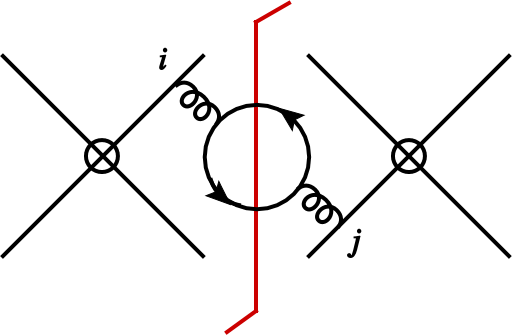
\includegraphics[width=0.30\textwidth]{plots/sf-nnlo-nf.png}
    \hfill
    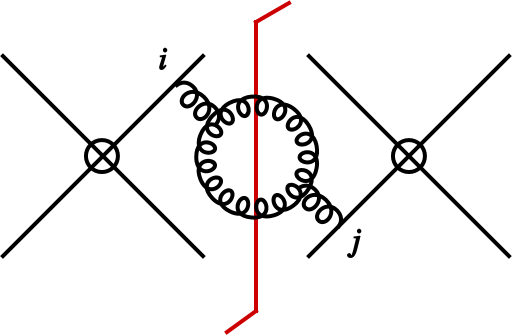
\includegraphics[width=0.30\textwidth]{plots/sf-nnlo-gluon.png}
    \hfill
    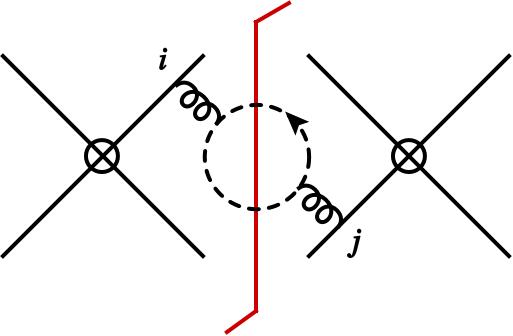
\includegraphics[width=0.30\textwidth]{plots/sf-nnlo-ghost.png}
  \end{center}
  \caption{Bubble diagrams contributing the NNLO soft function.
  }
  \label{fig:bubble-graphs}
\end{figure}

The second group consists of non-bubble graphs in which the gluons attach to
only two distinct Wilson lines: $i$ an $j$.
%
These graphs are shown in Fig.~\ref{fig:2WL2cut}.  We see that they
include both abelian and non-abelian structures.

\begin{figure}[t]
  \begin{center}
    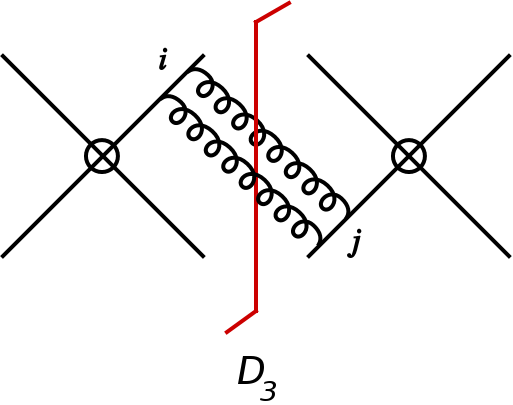
\includegraphics[width=0.30\textwidth]{plots/sf-nnlo-2cut.png}
    \hfill
    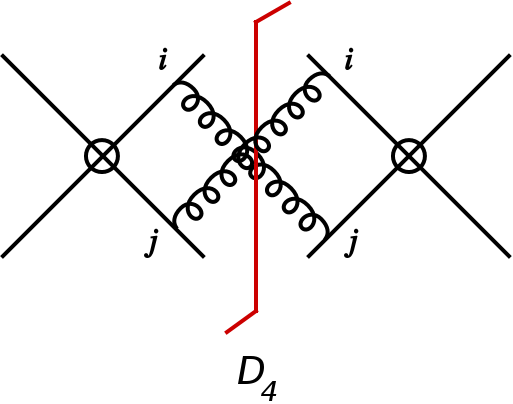
\includegraphics[width=0.30\textwidth]{plots/sf-nnlo-d4.png}
    \hfill
    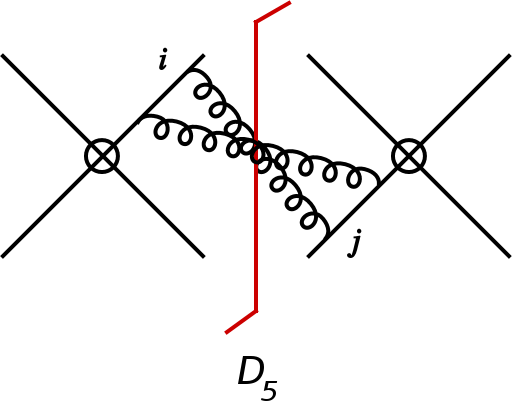
\includegraphics[width=0.30\textwidth]{plots/sf-nnlo-d5.png}
    \hfill
    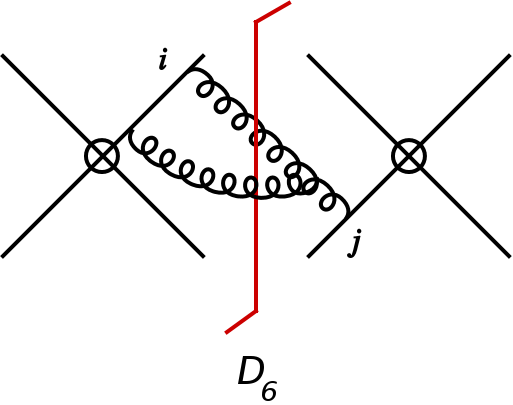
\includegraphics[width=0.30\textwidth]{plots/sf-nnlo-d6.png}
    \hspace{30pt}
    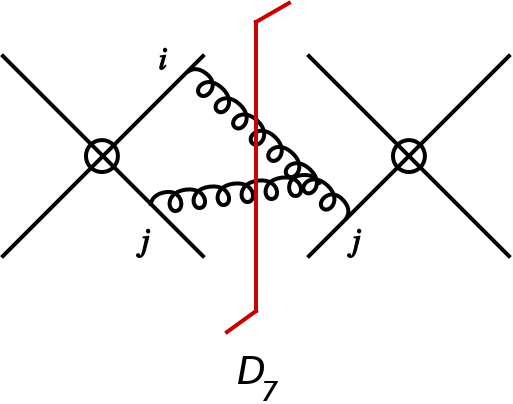
\includegraphics[width=0.30\textwidth]{plots/sf-nnlo-3gv.png}
  \end{center}
  \caption{Two-Wilson-line, double-cut diagrams required for the calculation of
  the NNLO soft function.
  }
  \label{fig:2WL2cut}
\end{figure}

The third group is formed by the three-Wilson-line, double-cut  diagrams shown
in Fig.~\ref{fig:3WL2cut}. 
%
The sum of the integral corresponding to $D^{(a)}_8$ and
its complex conjugate produce an integral which is a convolution of two NLO
expressions. Exactly the same expression is obtained when $D^{(b)}_8$ and
$D^{(c)}_8$ are added to their complex conjugates. And all the sums 
$D^{(i)}_8 + D^{(i)*}_8 $, for $i = a,b$ or $c$, are multiplied by the same colour factor
 $\{\cT_i^a, \cT_i^b\} \cT_j^a \cT_k^b$. 
%
The above observations were also made in the related calculation of the NNLO
soft function for top pair production in the threshold
limit~\cite{Ferroglia:2012uy, Wang:2018vgu}.

The abelian graphs depicted in Fig.~\ref{fig:3WL2cut} constitute the only
non-vanishing three-Wilson-line contribution in the group of double-cut diagrams.
This is because the non-abelian, three-Wilson-line graphs cancel when summed
over colour structures, which can be understood by analyzing the graph depicted
in Fig.~\ref{fig:3WLNA}. 
%
Since it is a double-cut diagram, the corresponding integral is a real-valued
function. And it is multiplied by the colour factor $i f^{abc}\cT^a_i T^b_j
T^c_k$. The complete soft function receives also a contribution from a diagram
which is a complex conjugate of Fig.~\ref{fig:3WLNA} and the complex
conjugation only affects the colour factor, turning it into $-i f^{abc}\cT^a_i
T^b_j T^c_k$.
%
Hence, the diagram of Fig.~\ref{fig:3WLNA} and its complex
conjugate cancel, and the non-abelian graphs with three distinct Wilson lines
connected by the gluons do not contribute to the soft function.

We emphasize that this happens only because the integrals are real
functions, as they originate from double-cut diagrams. This property will not be
true for single-cut, non-abelian diagrams, and we will see that the
corresponding contributions do not vanish when summed over all diagrams.

\begin{figure}[t]
  \begin{center}
    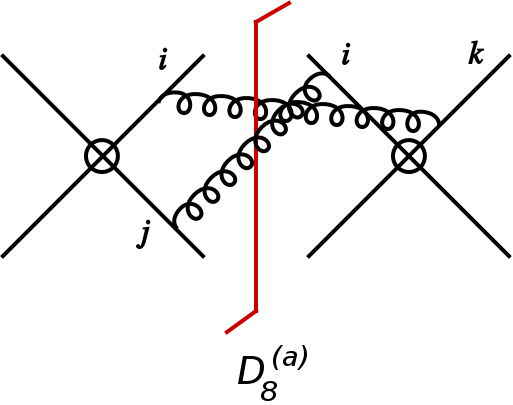
\includegraphics[width=0.30\textwidth]{plots/sf-nnlo-d8a.png}
    \hfill
    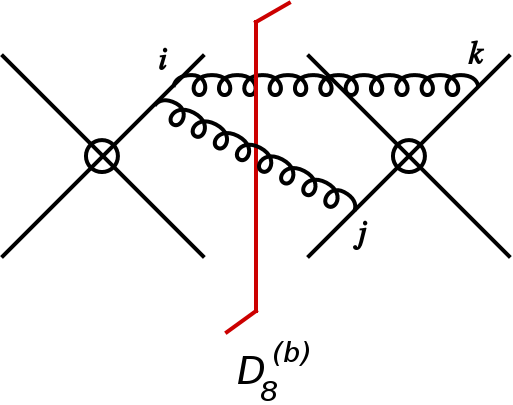
\includegraphics[width=0.30\textwidth]{plots/sf-nnlo-d8b.png}
    \hfill
    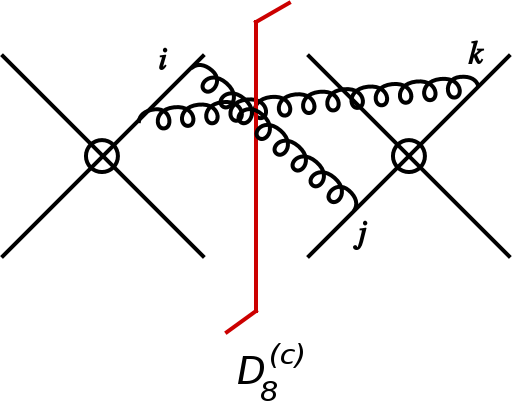
\includegraphics[width=0.30\textwidth]{plots/sf-nnlo-d8c.png}
  \end{center}
  \caption{Three-Wilson-line, double-cut diagrams required for the calculation
  of the NNLO soft function.
  }
  \label{fig:3WL2cut}
\end{figure}

\begin{figure}[t]
  \begin{minipage}[t]{0.48\textwidth}
  \begin{center}
    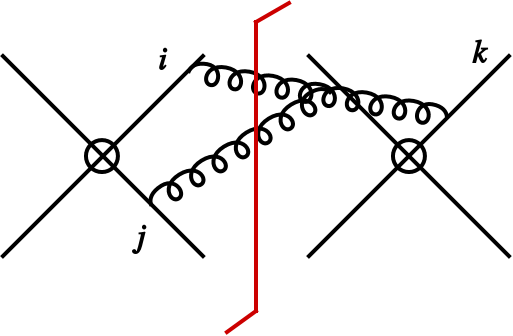
\includegraphics[width=0.625\textwidth]{plots/sf-nnlo-8prime.png}
  \end{center}
  \caption{Three-Wilson-line, double cut diagram appearing in the calculation of
  the NNLO soft function.
  }
  \label{fig:3WLNA}
  \end{minipage}
  \hfill
  \begin{minipage}[t]{0.48\textwidth}
  \begin{center}
    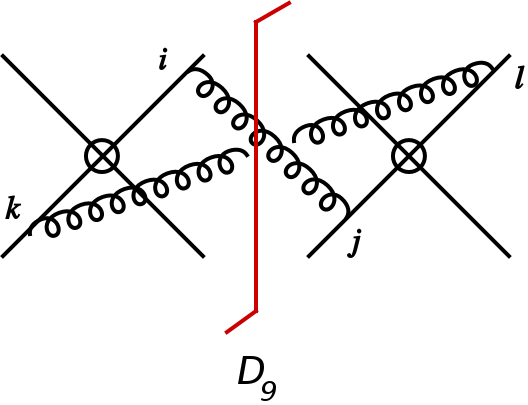
\includegraphics[width=0.625\textwidth]{plots/sf-nnlo-4wl.png}
  \end{center}
  \caption{Four-Wilson-line, double cut diagram required in the calculation of
  the NNLO soft function.
  }
  \label{fig:4WL2cut}
  \end{minipage}
\end{figure}

Finally, the double-cut part of the soft functions receives contributions from a
subset of diagrams shown in Fig.~\ref{fig:4WL2cut}, where the gluons connect
four distinct Wilson lines. The corresponding expressions take forms of
convolutions of the NLO integrals, similarly to the cases of $D_4$ and $D_8$
from Fig.~\ref{fig:2WL2cut} and \ref{fig:3WL2cut}.  
The four-Wilson-line diagrams come with the colour operator
$\cT_i^a \cT_j^a \cT_k^b \cT_l^b$. 

The complete expression for the NNLO soft function derived using the
diagrammatic approach described above can be obtained alternatively by taking
the soft limit of the relevant matrix elements in QCD. 

In the case of the $gg$ final state, in the limit $k, l \to 0$, the squared
matrix element factorizes as~\cite{Czakon:2014oma}
%
\begin{align}
\cm^{*(0)}_{g,g,a_1,\dots}(k,l,p_1,\dots)\,
\cm^{(0)}_{g,g,a_1,\dots}(k,l,p_1,\dots)
\hspace{-120pt}
&
\nonumber \\[0.5em]
\simeq \
&
\frac{1}{2}\sum_{ijkl}{\cal S}_{ij}(k){\cal S}_{kl}(l) \,
\la\cm^{(0)}_{a_1,\dots}(p_1,\dots)|
\left\{\cT_i\cdot\cT_j, \cT_k\cdot\cT_l\right\} 
|\cm^{(0)}_{a_1,\dots}(p_1,\dots)\ra
\nonumber \\
&
-C_A\sum_{ij}{\cal S}_{ij}(k,l) \,
\la\cm^{(0)}_{a_1,\dots}(p_1,\dots)|\cT_i\cdot\cT_j
|\cm^{(0)}_{a_1,\dots}(p_1,\dots)\ra\,,
\label{eq:2cutmaster}
\end{align}
%
where ${\cal S}_{ij}(k)$ is the eikonal integrand
%
\begin{equation}
  {\cal S}_{ij}(k) = \frac{p_i \cdot p_j}{(p_i \cdot k)\, (p_j\cdot k)}\,,
  \label{eq:eikfun}
\end{equation}
%
which we had used to construct the NLO soft function integrals in
Eq.~(\ref{eq:soft-func-nlo-mom-space-ddim}), and $p_i$ are the $d$-momenta of
the external partons. 
%
We note that the functions ${\cal S}_{ij}(k)$ and ${\cal S}_{ij}(k,l)$ are
invariant with respect to rescalings of the momenta of external particles of the
Born process.  Therefore, they can be expressed in terms of velocities
%
\begin{equation}
  n_i = 
  \left\{
  \begin{array}{l}
     n     \quad \text{for} \quad    i = 1\, \\
     \nbar \quad \text{for} \quad    i = 2\, \\
     \tilde v_i   \quad \text{for} \quad \! i = 3, 4\,
  \end{array}
  \right..
  %\label{eq:}
\end{equation}
%
The function ${\cal S}_{ij}(k,l)$ can be split into two parts
%
\begin{equation}
  \label{eq:soft}
  {\cal S}_{ij}(k,l) = {\cal S}^{m=0}_{ij}(k,l) + \left( m_i^2
  \; {\cal S}^{m \neq 0}_{ij}(k,l) + m_j^2 \; {\cal S}^{m \neq
    0}_{ji}(k,l) \right) \; ,
\end{equation}
%
where $m_i$ and $m_j$ are the masses of the external particles.
%
The first term in Eq.~(\ref{eq:soft}) has been given in
Ref.~\cite{Catani:1999ss} and reads
%
\begin{eqnarray}
  %\label{eq:}
{\cal S}^{m=0}_{ij}(k,l) &=& \frac{(1-\epsilon)}{(k \cdot l)^2}
\frac{p_i \cdot k \; p_j \cdot l + p_i \cdot l \; p_j \cdot
  k}{p_i \cdot (k+l) \; p_j \cdot (k+l)} \nonumber
\\ \nonumber \\
&& - \frac{(p_i \cdot p_j)^2}{2 \; p_i \cdot k \; p_j \cdot l \; p_i
  \cdot l \; p_j \cdot k} \left[ 2 - \frac{p_i \cdot k \; p_j
    \cdot l + p_i \cdot l \; p_j \cdot k}{p_i \cdot (k+l) \;
    p_j \cdot (k+l)} \right] \nonumber \\  \nonumber \\
&& + \frac{p_i \cdot p_j}{2 \; k \cdot l} \left[ \frac{2}{p_i
    \cdot k \; p_j \cdot l} + \frac{2}{p_j \cdot k \; p_i \cdot
    l} - \frac{1}{p_i \cdot (k+l) \; p_j \cdot (k+l)}
  \right. \nonumber \\ \nonumber \\
&& \times \left. \left( 4 + \frac{(p_i \cdot k \; p_j \cdot l +
    p_i \cdot l \; p_j \cdot k)^2}{\; p_i \cdot k \; p_j \cdot
    l \; p_i \cdot l \; p_j \cdot k} \right) \right] \; .
    \label{eq:Smassless}
\end{eqnarray}
%
In the above equation, the first line comes solely from the gluon and ghost
bubble diagrams of Fig.~\ref{fig:bubble-graphs}. The second line originates from
the $C_A$ part of diagrams which do not involve the triple-gluon vertex, that
is $D_4$ and $D_5$ in Fig.~\ref{fig:2WL2cut}. Finally, the last two lines
receive contributions from the non-abelian diagrams $D_6$, $D_7$ and the gauge
bubble.

The second contribution in Eq.~(\ref{eq:soft}) was derived in
Ref.~\cite{Czakon:2011ve} and represents additional terms generated by
non-vanishing masses. The relevant function is
%
\begin{eqnarray}
  {\cal S}^{m\neq0}_{ij}(k,l) &=
  &  - \frac{1}{4  \; k \cdot l \; p_i \cdot
  k \; p_i \cdot l} + \frac{p_i \cdot p_j \; p_j
  \cdot (k+l)}{2 \; p_i \cdot k \; p_j \cdot l \; p_i \cdot l \;
    p_j \cdot k \; p_i \cdot (k+l)} \nonumber \\ \nonumber \\
  && - \frac{1}{2 \; k \cdot l \; p_i \cdot (k+l) \; p_j \cdot
    (k+l) } \left( \frac{(p_j \cdot k)^2}{p_i \cdot k \; p_j
    \cdot l} + \frac{(p_j \cdot l)^2}{p_i \cdot l \; p_j \cdot
    k} \right) \; . \nonumber \\
    \label{eq:Smassive}
\end{eqnarray}
%
Here, the first and the third term come from the $C_A$ part of diagrams
which do not involve the triple-gluon vertex, whereas the second term arises due to
non-abelian contributions, including the gauge bubble.

In the case of the final-state $q{\bar q}$-pair, in the limit $k, l \to 0$, the
matrix element factorizes as~\cite{Czakon:2014oma}
%
\begin{align}
  \label{qqsoftfac}
  \cm^{*(0)}_{q,{\bar q},a_1,\dots}(k,l,p_1,\dots)\,
  \cm^{(0)}_{q,{\bar q},a_1,\dots}(k,l,p_1,\dots) 
  &  
  \nonumber \\[0.5em]
  &
  \hspace{-100pt}
  \simeq
  T_F \sum_{ij} {\cal I}_{ij}(k,l) \,
  \la \cm^{(0)}_{a_1,\dots}(p_1,\dots)|\cT_i \cdot
  \cT_j|\cm^{(0)}_{a_1,\dots}(p_1,\dots)\ra\; ,
\end{align}
% 
where the function $ {\cal I}_{ij}(k,l)$ has the form
%
\begin{equation}
  \label{eq:Iij1}
  {\cal I}_{ij}(k,l) = \frac{(p_i \cdot k)\, (p_j \cdot l)
  + (p_j \cdot k)\, (p_i \cdot l) - (p_i \cdot p_j) 
  \,(k \cdot l)}{(k \cdot l)^2 
  \,[p_i\cdot (k+l)]\, [p_j \cdot (k+l)]} \,.
\end{equation}

The above expressions can be used directly to calculate our soft function of
interest by applying the following formula
%
\begin{align}
  \bfS_{i\bar i}^{(2), f\bar f} (q_\perp) & = 
   (4\pi)^4
  \left(\frac{\mu^2 e^{\gamma_E}}{4\pi}\right)^{2\epsilon}\!\!\!\!\nu^{2\alpha}
  \frac{(2\pi)^{\frac{d}{2}-1}}{ S_{d-3} \,q_T^{d-3}}
  \int 
  \frac{d^d\, \delta_+(k^2)}{(2\pi)^{d-1} (n\cdot k)^\alpha}\, \frac{d^d l\,
  \delta_+(l^2)}{(2\pi)^{d-1}(n\cdot l)^\alpha}\; 
    \delta(q_\perp- | k_\perp+l_\perp |)\,
  \nonumber \\
  &
  \hspace{40pt}
  \times
  \langle c_I^{i\bar i} | 
  \cm^{*\, (0)}_{f,\bar f,a_1,\dots}(k,l,p_1,\dots)
  \cm^{(0)}_{f,\bar f,a_1,\dots}(k,l,p_1,\dots)
  |c_J^{i\bar i} \rangle\,,
  \label{eq:S2cutfromM22cut}
\end{align}
%
where the case with $f=q$ corresponds to the $q\bar q$ final state while
the case with $f=g$ corresponds to the $gg$ final state.

We have checked through direct calculation that the expression for the NNLO soft
function  derived using definitions given in
Eqs.~(\ref{eq:Wdef})-(\ref{eq:Osggdef}), \ie expanding the Wilson lines and
truncating the series at $\order{\as^2}$, matches exactly the 
formula (\ref{eq:S2cutfromM22cut}).

To complete the definition of Eq.~(\ref{eq:S2cutfromM22cut}), we need to specify
the colour matrices $\bm{w}_{ij}^{(1)}$ and $\bm{w}_{ijkl}^{(2S)}$, following
Eq.~(\ref{eq:w1w2def}).  
%
The matrices $\bm{w}_{ij}^{(1)}$, built from products of two colour operators,
are identical with those found in the calculation of the NLO soft function.
%
The matrices $\bm{w}_{ijkl}^{(2S)}$, constructed from the anticommutator,
involve products of four colour operators, and appear for the first time at
NNLO.
%
The complete set of the $\bm{w}_{ij}^{(1)}$ and $\bm{w}_{ijkl}^{(2S)}$ matrices,
in both the $q\bar q$ and the $gg$ channel, is given in
Appendix~\ref{app:colmat}.

%-----------------------------------------------------------------------------
\subsubsection*{Single-cut diagrams}

\begin{figure}[t]
  \begin{center}
    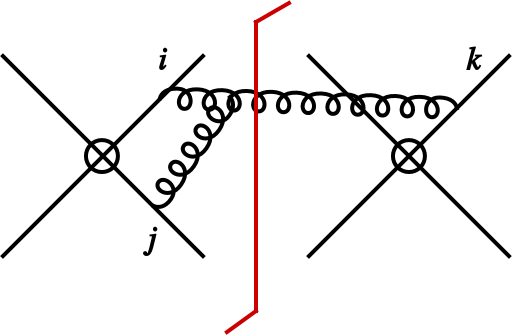
\includegraphics[width=0.30\textwidth]{plots/sf-nnlo-real-virtual1.png}
    \hfill
    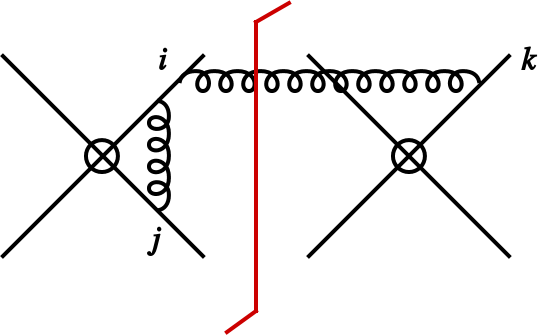
\includegraphics[width=0.30\textwidth]{plots/sf-nnlo-real-virtual2.png}
    \hfill
    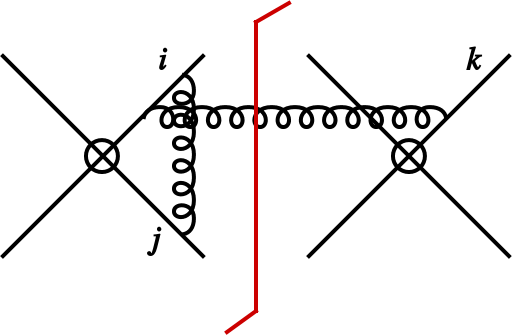
\includegraphics[width=0.30\textwidth]{plots/sf-nnlo-real-virtual3.png}
  \end{center}
  \caption{
  Single-cut diagrams contributing to the NNLO soft function.
  }
  \label{fig:1cutdiagrams}
\end{figure}

The single-cut diagrams required for the calculation of the NNLO soft function
for top pair production are shown in Fig.~\ref{fig:1cutdiagrams}. In this
class of graphs, one gluon is real and the other runs in a loop. Because of the
latter, the integrals from the single-cut graphs produce also an imaginary
contribution.

As in the case of the double-cuts , also the single-cut term derived
using the diagrammatic approach described above can be obtained alternatively by
taking the soft limit of the relevant matrix elements in QCD. This results
in the formula~\cite{Bierenbaum:2011gg}
%
\begin{align}
  &
  \hspace{-50pt}
  \cm^{*\, (1)}_{g ,a_1,\dots}(k,p_1,\dots)
  \cm^{(0)}_{g ,a_1,\dots}(k,p_1,\dots) + \text{c.c.}
  \nonumber \\[0.5em]
  & = - 
  \Bigg[ 
    2C_A\sum_{i\neq j = 1}^n
    \left(e_{ij}-e_{ii}\right) R_{ij}\langle M^{(0)}(n) 
    \vert \cT_i\cdot \cT_j \vert
    M^{(0)}(n)  \rangle  
    \nonumber \\
    & \hspace{70pt}
    -  4\pi\!\!\sum_{i\neq j\neq k = 1}^n e_{ik}I_{ij} \langle
    M^{(0)}(n)\vert  f^{abc} \cT_i^a \cT_j^b \cT_k^c \vert M^{(0)}(n)  \rangle
  \Bigg]\,,
  \label{eq:1cutmaster}
\end{align}
%
where
%
\begin{equation}
  \label{eq:eikprop}
  e_i^\mu = \frac{p_i^\mu}{p_i \cdot k}\,,
\end{equation}
%
while $ R_{ij}$ and $I_{ij}$ correspond to the real and imaginary parts
from integration over the loop momentum and they were obtained in
Refs.~\cite{Bierenbaum:2011gg, Czakon:2018iev}.  We notice that a new,
antisymmetric colour structure appears in the imaginary part:
$if^{abc} \cT_i^a \cT_j^b \cT_k^c  = [\cT_i \cdot \cT_k, \cT_j \cdot \cT_k]$.
%
The corresponding colour matrix $\bm{w}_{ijk}^{(2A)}$ is defined in
Eq.~(\ref{eq:w3def}) and its explicit expressions are given in
Appendix~\ref{app:colmat}.

We have checked through direct calculation, based on definitions given in
Eqs.~(\ref{eq:Wdef})-(\ref{eq:Osggdef}), that we reproduce the single-cut
expression of Eq.~(\ref{eq:1cutmaster}). With the latter, we can then
determine the real-virtual part of our soft function
%
\begin{align}
  \bfS_{i\bar i}^{(2), g} (q_\perp) & = 
   (4\pi)^4
  \left(\frac{\mu^2 e^{\gamma_E}}{4\pi}\right)^{2\epsilon}
  \!\!\!\!\nu^{\alpha}
  \frac{(2\pi)^{\frac{d}{2}-1}}{ S_{d-3}\,q_T^{d-3}}
  \int \! \, \frac{d^d k \,\delta_+(k^2) }{(2\pi)^{d-1} (n\cdot k)^\alpha} 
   \; \delta(q_\perp-k_\perp)\,
  \nonumber \\
  &
  \hspace{40pt}
  \times
  \langle c_I^{i\bar i} | 
  \cm^{*\, (1)}_{g ,a_1,\dots}(k,p_1,\dots)
  \cm^{(0)}_{g ,a_1,\dots}(k,p_1,\dots) + \text{c.c.}\,
  |c_J^{i\bar i} \rangle\,.
  \label{eq:S2cutfromM21cut}
\end{align}
%

%-----------------------------------------------------------------------------
\subsubsection*{Zero-cut diagrams}

Purely virtual, two-loop diagrams, do not involve a cut gluon. Therefore, the
measurement function $\delta^{(d-2)}(f(k,l) - q_\perp)$ does not appear in the
corresponding integrals. As a consequence, these integrals are scaleless and
vanish in dimensional regularization. Hence, the NNLO soft function for top
pair production does not receive contributions from two-loop diagrams.

%-----------------------------------------------------------------------------
\subsection{Symmetries between integrals}
\label{sec:intsym}

Our double-cut, soft function integrals have the general structure
%
\begin{align}
  \tilde I(\{p_i, p_j\}) &= \int d^dk\, d^d l\, \delta^{(+)}(k^2)
  \delta^{(+)}(l^2) h(p_i\cdot p_j, p_i\cdot k, p_i \cdot l)\,
  \delta^{(d-2)}(k_\perp+l_\perp -q_\perp)\,,
  \label{eq:Isymmetry}
\end{align}
%
where $p_i$ are the momenta of external particles.

The above integral can depend only on the scalar productions $p_i \cdot p_j$,
which are invariant with respect to Lorentz transformations 
$p^\mu \to \Lambda^\mu{}_\nu\, p^\nu$. 
To balance the transformation of the
external momenta in the scalar products $p_i \cdot k$ and $p_i \cdot l$ one
needs to transform the gluon momenta $k$ and $l$ with
$\left(\Lambda^{-1}\right)^\mu{}_\nu$. 
%
This, however, does not leave the integral unchanged for a general Lorentz
transformation because of the transverse delta function appearing in
Eq.~(\ref{eq:Isymmetry}).
%
Therefore, the integral $\tilde I(\{p_i, p_j\})$ is invariant
only under a subgroup of the Lorentz group which involves:
%
\begin{itemize}
  %\setlength\itemsep{1.2em}
  \item
  rescaling of the light-cone components of the momenta $k$ and $l$ compensated
  by inverse rescaling of the light-cone components of the external momenta,
  \item
  rotations of the above momenta in the transverse plane such that 
  $|k_\perp + l_\perp| = q_T$.
\end{itemize}
%
Let us denote
\begin{align}
  p\cdot q & \qquad 
  \text{usual, $d$-dimensional scalar product}, \\
  p * q & = p_0 q_0 - p_3 q_3 = p_+ q_- + p_- q_+\,.
\end{align}


Given the above reduced Lorentz symmetry, and the fact that the result can
only depend on external momenta, we conclude, that our integral must be a
function of $p_i * p_j$ and $p_{i,\perp} \cdot p_{j,\perp}$ or, equivalently,
$p_i * p_j$ and $p_i \cdot p_j$.

As is clear from Eqs.~(\ref{eq:eikfun})-(\ref{eq:Iij1}), the integrand is
invariant under the rescaling of $p_3 = \lambda_3 p_3$ and $p_4 = \lambda_4
p_4$, for arbitrary $\lambda$, which means that the result can only be a
function of ratios of the above scalar products.

Integrals which do not exhibit $\alpha$ poles are, in addition, invariant under
rescaling of $p_1$. But, here, one cannot form a variable of the type $p_1
\cdot p_3/\sqrt{p_1^2 p_3^2}$ because $p_1$ is massless. As a consequence, the
only possibility is $p_3*p_3/p_3^2 = p_4*p_4/p_4^2 $. 
This is why some abelian integrals are equal. 
%
In the cases of the integrals with $\alpha$ poles, rescaling of $p_1$ is broken
by the analytic regulator: $I(\lambda p_1) =  \lambda^{-\alpha} I(p_1)$.


%-----------------------------------------------------------------------------
\subsection{Differential equations approach and bubble diagrams}
\label{sec:debubble}

\begin{figure}[t]
  \begin{center}
    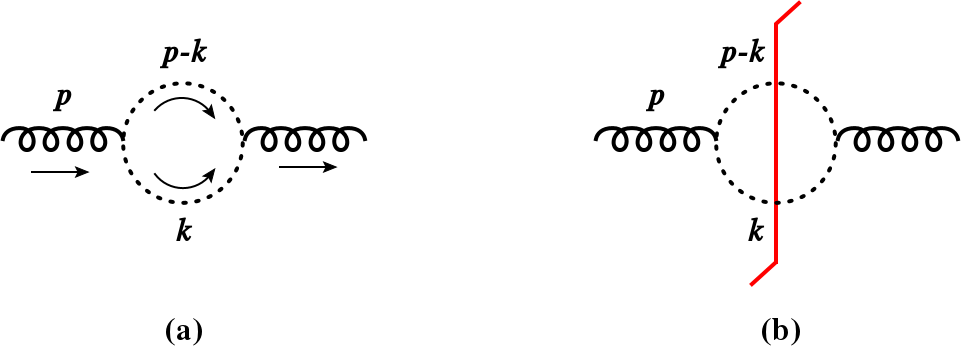
\includegraphics[width=0.62\textwidth]{plots/vp-diagram.png}
  \end{center}
  \caption{
  Gluon vacuum polarization diagram (a) and its cut counterpart (b).
  Dashed lines correspond to either a quark, a gluon or a ghost.
  }
  \label{fig:vp-diagram}
\end{figure}

With an exception of the propagators introduced to regularize rapidity
divergences, the quark, gluon and ghost bubble, as well as part of the triple
gluon vertex diagrams depicted in Fig.~\ref{fig:2WL2cut}, which we shall call
``tadpole'', depend only on the
momenta $k$ and $k+l$.
%
This feature allows one to first integrate over $k+l$ and then solve the
integral over $k$ with help of the differential equation 
approach~\cite{Kotikov:1990kg, Remiddi:1997ny}. The integration
can be performed mostly analytically, with an exception of a few one-dimensional
integrals which we integrate by numerical methods.

%-----------------------------------------------------------------------------
\subsubsection{Vacuum polarization tensor}

We consider the process depicted in Fig.~\ref{fig:vp-diagram}~(a), where the
particle running in the loop can be a quark, a gluon or a ghost. The
corresponding vacuum polarization integrals read 
%
\begin{equation}
  \im \Pi^{\mu\nu}(\alpha) = 
  C_f \frac{g^2}{16}\, e^{\epsilon \gamma_E} \mu^{2\epsilon} \nu^{2\alpha}
  \pi^{-4+\epsilon}
  \int d^d k \frac{N^{\mu\nu}(k,p)}{
  \left(k\cdot n\right)^\alpha\, 
  \left(p\cdot n - k\cdot n\right)^\alpha\, k^2\, (p-k)^2}\,,
  \label{eq:ImPiint}
\end{equation}
%
where $C_f = C_A$ for the gluon bubble and the tadpole, while $C_f=-T_F$ for
the quark bubble.  The numerator $N^{\mu\nu}(k,p)$ depends on the particle in
the loop.
%
For the quark loop we have
%
% NOTE
% ttbar/vp-terms/vacuum-polarization.nb
%
\begin{eqnarray}
  N^{\mu\nu} = 
    8\, k^\mu k^\nu
    -4k^\mu p^\nu 
    -4p^\mu k^\nu 
    -4g^{\mu\nu} k^2 
    +4g^{\mu\nu} k\cdot p\,,
  %\label{eq:}
\end{eqnarray}
%
for the gluon+ghost loop
%
\begin{eqnarray}
  N^{\mu\nu} & =  &
    (2d-4)\, k^\mu k^\nu +
    \frac{2d-3}{2}\, k^\mu p^\nu +
    \frac{2d-5}{2}\, p^\mu k^\nu +
    \frac{d-6}{2}\, p^\mu p^\nu 
  \nonumber \\
  & & 
   + g^{\mu\nu}\, k^2 +
    g^{\mu\nu}\, k\cdot p +
    \frac{5}{2}\, g^{\mu\nu} p^2\,,
  %\label{eq:}
\end{eqnarray}
%
and for the tadpole
%
\begin{eqnarray}
  N^{\mu\nu} = - 4 g^{\mu\nu} p^2\,.
  %\label{eq:}
\end{eqnarray}
%
The directions of momenta are indicated with arrows in
Fig.~\ref{fig:vp-diagram}~(a).

All propagators are assumed to be defined with the $+i\epsilon$ prescription.
%
The most generic self-energy tensor that can be formed out the $d$-vectors $p$
and $n$, and the metric tensor $g^{\mu\nu}$ is
%
\begin{equation}
  \im \Pi^{\mu\nu}(\alpha) = 
  T_{00}\, g^{\mu\nu} +
  T_{pp}\, p^{\mu}p^{\nu} +
  T_{nn}\, n^{\mu}n^{\nu} +
  T_{pn}\, \left(n^{\mu} p^{\nu}+p^{\mu} n^{\nu}\right)\,.
  \label{eq:ImPi}
\end{equation}
%
The coefficients $T_{ij}$ can be expressed in terms of two scalar integrals,
$A_0$ and $B_0$, through the procedure of Passarino-Veltman
reduction~\cite{Passarino:1978jh}
%
\begin{align}
  A_0^{(a)}(\alpha_1,\alpha_2) &= 
  \int\frac{d^d k}{(n\cdot k)^{\alpha_1}\, (n\cdot (p+k))^{\alpha_2}\, k^2}\,,
  \\[0.5em]
  B_0^{(a)}(\alpha_1,\alpha_2) &= 
  \int\frac{d^d k}{(-n\cdot k)^{\alpha_1}\, (n\cdot (p+k))^{\alpha_2}\, k^2\,
  (p+k)^2}\,.
  %\label{eq:}
\end{align}
%
The integral $A_0$ can be shown to be scaleless and, therefore, it
vanishes. Hence, it turns out that the only two-point integral that we need to
determine $\im \Pi^{\mu\nu}$ is $B_0$, and this integral can be
calculated exactly by means of Schwinger parametrization. The result takes the
form
%
% NOTE
% ttbar/vp-terms/vacuum-polarization.nb
%
\begin{equation}
  B_0^{(a)}(\alpha_1,\alpha_2) = 
  i \pi ^{\frac{d}{2}}\,
  \frac{\Gamma (\epsilon ) \Gamma (1-\alpha_1 -\epsilon )  
        \Gamma (1-\alpha_2 -\epsilon )}
  {\Gamma (2-\alpha_1 -\alpha_2 -2\epsilon)}\,
  \left(-p^2\right)^{-\epsilon }\, (n \cdot p)^{-\alpha_1 - \alpha_2 }\,.
  \label{eq:B0virt}
\end{equation}
%
Unitarity allows us to obtain also a version of this function which
corresponds to the cut diagram of Fig.~\ref{fig:vp-diagram}~(b)
%
% NOTE
% above B_0^{(a)} /. (-q^2)^-ep -> 2 I Sin[Pi ep] q^(-2 ep)
%
\begin{equation}
  B_0^\text{(b)}(\alpha_1,\alpha_2) = 
  -2 \pi ^{\frac{d}{2}}\,
  \frac{\Gamma (\epsilon ) \Gamma (1-\alpha_1 -\epsilon )  
        \Gamma (1-\alpha_2 -\epsilon )}
  {\Gamma (2-\alpha_1 -\alpha_2 -2\epsilon)}\,
  \sin (\pi  \epsilon )\,
  p^{-2 \epsilon }\, (n \cdot p)^{-\alpha_1 - \alpha_2 }\,.
  \label{eq:B0real}
\end{equation}
%
Finally, the coefficients in Eq.~(\ref{eq:ImPi}) take the following forms. For
the quark bubble
%
\begin{align}
  \label{eq:Tijquark}
  T_{00} &= \frac{2 \left(2 (1-\epsilon)^2-\alpha  (1-2 \epsilon)\right)}
  {(1-\epsilon) (3-2 \alpha -2 \epsilon)}
  \, \tilde B_0(\alpha)\, p^2\,,
  &\quad
%  \,,\\
  %
  T_{pp} &= -\frac{4 (1-\alpha -\epsilon)}{3-2 \alpha -2 \epsilon} 
  \, \tilde B_0(\alpha)\,, \\
  %
  T_{nn} &= 
  \frac{2 \alpha }{(1-\epsilon) (3-2 \alpha -2 \epsilon)}
  \, \tilde B_0(\alpha)\,
  \frac{p^4}{\left(n\cdot p\right)^2}\,,
  &\quad
%  \,,\\
  %
  T_{pn} &= 
  -\frac{2 \alpha}{(1-\epsilon) (3-2 \alpha -2 \epsilon) }
  \, \tilde B_0(\alpha)\,
  \frac{p^2}{n\cdot p}
  \,,
  \nonumber
\end{align}
%
with
%
\begin{equation}
  \tilde B_0(\alpha) = -\frac{g^2}{16} T_F 
  \frac{e^{\epsilon\gamma_E}\mu^{2\epsilon}\nu^{2\alpha}}{\pi^{4-\epsilon}}
  B_0(\alpha,\alpha)\,.
  \label{eq:tB0quark}
\end{equation}
%
For the gauge (\ie gluon + ghost) bubble
%
\begin{align}
  T_{00} &= 
  \frac{5 - 3 \alpha - 3 \epsilon}{3 - 2 \alpha - 2 \epsilon}
  \, \tilde B_0(\alpha)\, p^2\,,
  &\quad
  %
  T_{pp} &= \frac{-5 + 4 \alpha + 3 \epsilon}{3 - 2 \alpha - 2 \epsilon}  
  \, \tilde B_0(\alpha)\,, \\
  %
  T_{nn} &= 
  \frac{\alpha }{3 - 2 \alpha - 2 \epsilon}
  \, \tilde B_0(\alpha)\,
  \frac{p^4}{\left(n\cdot p\right)^2}\,,
  &\quad
  %
  T_{pn} &= 
  -\frac{\alpha}{3 - 2 \alpha - 2 \epsilon }
  \, \tilde B_0(\alpha)\,
  \frac{p^2}{n\cdot p}
  \,,
  \nonumber
\end{align}
%
with
%
\begin{equation}
  \tilde B_0(\alpha) = 
  \frac{g^2}{16} C_A 
  \frac{e^{\epsilon\gamma_E}\mu^{2\epsilon}\nu^{2\alpha}}{\pi^{4-\epsilon}}
  B_0(\alpha,\alpha)\,.
  \label{eq:tB0gauge}
\end{equation}
%
And for the tadpole
%
\begin{align}
  T_{00} &= 
  -\frac{g^2}{4} C_A 
  \frac{e^{\epsilon\gamma_E}\mu^{2\epsilon}\nu^{2\alpha}}{\pi^{4-\epsilon}}\,
  B_0(\alpha,\alpha)\, p^2\,,
  &\quad
  %
  T_{pp} &= 0 \,, 
  &\quad
  %
  T_{nn} &= 0 \,,
  &\quad
  %
  T_{pn} &= 0 \,.
  \label{eq:Tijtadpole}
\end{align}
%
The function $B_0(\alpha,\alpha)$ in Eqs.~(\ref{eq:tB0quark}),
(\ref{eq:tB0gauge}) and (\ref{eq:Tijtadpole}) can be given either by
Eq.~(\ref{eq:B0virt}) or by Eq.~(\ref{eq:B0real}). In our soft function
calculation, we will use the latter, cut version of this two-point integral.

One can check that the results given in this section recover standard
expressions for the gluon vacuum polarization tensor in the limit $\alpha \to
0$, where, in particular, the coefficients $T_{nn}$ and $T_{pn}$ vanish.

%-----------------------------------------------------------------------------
\subsubsection{Soft function integrals}

The above results for the quark and gauge bubble can now be embedded in the
two-Wilson-line soft function graphs, as depicted in
Fig.~\ref{fig:bubble-graphs}. 
%
The tadpole integrals correspond to the diagram $D_6$ of
Fig.~\ref{fig:2WL2cut} with the eikonal propagator connecting the two
gluons replaced by a pinch.
%
The integrals that appear have the following structure 
%
\begin{equation}
  I = \int\frac{d^d k\, \delta(k_T^2-1)\, \theta(k^2)\, \theta(k_0)}
      {(n\cdot k)^{a_1+2\alpha} (\nbar\cdot k)^{a_2} (v_3 \cdot k)^{a_3} (v_4
      \cdot k)^{a_4} (k^2)^{a_0+\epsilon}}\,.
  \label{eq:sfnf-general-structure}
\end{equation}

We note that, as in the case of the NLO soft function discussed in
Section~\ref{sec:NLOsf}, the integration measure can be written as $d^d k = d
k_+ d k_- d^{d-2} k_\perp$ and the $k_+$ and $k_-$ components are integrated
from minus to plus infinity.
%
However, the phase space of the integration over the light-cone momenta is
restricted, this time by $\theta(k^2)\, \theta(k^0) = \theta(k_+ k_- -
k_T^2)\, \theta(k_+ + k_-)$.  Because of the first theta function, the
integration is fixed not to a line, as in the case of the NLO soft function
depicted in Fig.~\ref{fig:light-cone-phase-space}~(left), but to the region
defined by the condition $k_+ k_- > k_T^2$, which means that $k_+$ and $k_-$
have to be both positive or negative.  The second theta function chooses
$k_+$ and $k_-$ to be both positive. 
%
Hence, the $d$-momentum of the off-shell gluon which appears in the bubble and
the tadpole diagrams is integrated over  the region depicted in
Fig.~\ref{fig:light-cone-phase-space}~(right).


We would like to solve the class of integrals from
Eq.~(\ref{eq:sfnf-general-structure}) by means of the method of differential
equations~\cite{Kotikov:1990kg, Remiddi:1997ny}, with help of
reverse unitarity~\cite{Anastasiou:2002yz}, which allows one to turn delta
functions into propagators.
%
What prevents us from direct use of the latter is the $\theta(k^2)$ function.
However, we can trade this theta function for the Dirac delta function at the
cost of introducing an extra integration over a spurious mass, $m^2$. Namely, we
multiply Eq.~(\ref{eq:sfnf-general-structure}) by 
%
\begin{equation}
  1 = \int_0^\infty dm^2 \delta(k^2-m^2)\,,
  %\label{eq:}
\end{equation}
%
which leads to
\begin{align}
  I & = \int_0^\infty dm^2 \delta(k^2-m^2)
      \int\frac{d^d k\, \delta(k_T^2-1)\, \theta(k^2)\, \theta(k_0)}
      {(n\cdot k)^{a_1+2\alpha} (\nbar\cdot k)^{a_2} (v_3 \cdot k)^{a_3} (v_4
      \cdot k)^{a_4} (k^2)^{a_0+\epsilon}}
    \nonumber \\
    & = \int_0^\infty dm^2 \delta(k^2-m^2)
      \int\frac{d^d k\, \delta(k_T^2-1)\, \theta(m^2)\, \theta(k_0)}
      {(n\cdot k)^{a_1+2\alpha} (\nbar\cdot k)^{a_2} (v_3 \cdot k)^{a_3} (v_4
      \cdot k)^{a_4} (m^2)^{a_0+\epsilon}}
    \nonumber \\
    & = \int_0^\infty \frac{dm^2}{(m^2)^{a_0+\epsilon}}\
      \int\frac{d^d k\, \delta(k_T^2-1)\,\delta(k^2-m^2)  \theta(k_0)}
      {(n\cdot k)^{a_1+2\alpha} (\nbar\cdot k)^{a_2} (v_3 \cdot k)^{a_3} (v_4
      \cdot k)^{a_4}}\,.
  \label{eq:IandIbardef}
\end{align}
%
Hence, we obtain
%
\begin{equation}
  I =\int_0^\infty \frac{dm^2}{(m^2)^{a_0+\epsilon}} \bar I (m^2)\,.
  \label{eq:Im2Ibar}
\end{equation}
%
Now we can use reverse unitarity to turn delta functions in $\bar I(m^2)$
into propagators, which leads to the following topology
%
\begin{align}
  \label{eq:topology-bubble}
  \bar I(a_1, a_2, a_3, a_4, a_5, a_6)  
  & =   \\[0.5em] 
  &  \hspace{-70pt}
  \int \frac{d^d k}
  {(n\cdot k)^{a_1+2\alpha} (\nbar\cdot k)^{a_2} (v_3 \cdot k)^{a_3} (v_4
  \cdot k)^{a_4} (k^2-m^2)^{a_5} ((n\cdot k)(\nbar \cdot k)-m^2-1)^{a_6}}\,.
  \nonumber
\end{align}

We observe that all $\epsilon$ poles, hence those of the soft origin,
are generated by performing the integral over~$m^2$ in Eq.~(\ref{eq:Im2Ibar})
while the function $\bar I(m^2)$ is finite in the limit $\epsilon \to 0$.

A set of identities can be derived for the class of integrals defined in
Eq.~(\ref{eq:topology-bubble}). First of all, $\bar I(a_1,a_2,\ldots, a_{6})$
obeys the standard integration by parts~(IBP) identities
%
\begin{eqnarray}
   \int d^dk\, \frac{\partial}{\partial k^\mu} q^\mu 
   \bar I(a_1,a_2,\ldots, a_{6}) & = & 0\,,
   %\label{eq:}
\end{eqnarray}
%
with $q^\mu = n^\mu, \nbar^\mu, v_3^\mu, v_4^\mu, k^\mu$. The set of IBPs
consists of five relations. In addition, the topology $\bar I$ exhibits certain
redundancies which result in additional identities. One of them comes from the
$q_T$-delta propagator
%
\begin{equation}
  \bar I\, \frac{(n\cdot k) (\nbar\cdot k) - m^2-1}
         {(n\cdot k) (\nbar\cdot k) - m^2-1}  = \bar I\,,
  %\label{eq:}
\end{equation}
%
which gives
%
\begin{equation}
  \bar I(a_1-1, a_2-1, a_3, a_4, a_5, a_6+1)  
  - (m^2+1) \bar I(a_1, a_2, a_3, a_4, a_5, a_6+1)   =
  \bar I(a_1, a_2, a_3, a_4, a_5, a_6)\,.
  %\label{eq:}
\end{equation}
%
The last identity arises from  momentum conservation following the
discussion of Section~\ref{sec:kinematics}
%
\begin{equation}
  n + \nbar = \tilde v_3 + \tilde v_4\,.
  %\label{eq:}
\end{equation}
Multiplying the above by $k$ leads to 
%
% NOTE
% ttbar/vp-terms/idsolver/ibps-nnlo.nb
%
\begin{align}
  \bar I(a_1, a_2, a_3-1, a_4, a_5, a_6) +
  \bar I(a_1, a_2, a_3, a_4-1, a_5, a_6) -
  \nonumber \\
  \bar I(a_1-1, a_2, a_3, a_4, a_5, a_6) -
  \bar I(a_1, a_2-1, a_3, a_4, a_5, a_6) & = 0\,.
  %\label{eq:}
\end{align}
%
Hence, altogether  we have  seven identities which we use to reduce all
the integrals appearing in the problem to a set of master integrals.

%
While solving the bubble graphs with the above method, it is important to note
that the $d$-vector $k^\mu$ in Eq.~(\ref{eq:topology-bubble}) is now massive.
Hence, the parametrization from Eq.~(\ref{eq:kparam}) does not hold
and it must be replaced with 
%
\begin{equation}
 k  = 
 (k_0, \ldots,
 |\vec k| \sin\theta_1\sin\theta_2, ,|\vec k| \sin\theta_1\cos\theta_2,
 |\vec k| \cos\theta_1)\,,
 \label{eq:k4v-par-massive}
\end{equation}
%
where
%
\begin{equation}
 |\vec k| = \sqrt{k_0^2-m^2}\,.
  %\label{eq:}
\end{equation}
%
Therefore, the relevant inner products now take the form
%
\begin{align}
  n \cdot k & =  k_0 - |\vec k| \cos\theta_1\,, \\
  \nbar \cdot k & =  k_0 + |\vec k| \cos\theta_1\,, \\
  \tilde v_3 \cdot k & =  k_0- 
  \beta_t\, |\vec k| \sin\theta_1\cos\theta_2\sin\theta -
  \beta_t\, |\vec k| \cos\theta_1\cos\theta\,, \\
  \tilde v_4 \cdot k & =  k_0+
  \beta_t\, |\vec k|\sin\theta_1\cos\theta_2\sin\theta +
  \beta_t\, |\vec k|\cos\theta_1\cos\theta\,.
\end{align}
%
We also get that
%
\begin{align}
 k_0 & = \frac12\left(n\cdot k + \nbar \cdot k\right) 
 = \frac12\left(\tilde v_3\cdot k + \tilde v_4 \cdot k\right)\,.
\end{align}

The complete bubble+tadpole-part of the NNLO soft function requires calculation
of the integrals which correspond to the diagrams of
Fig.~\ref{fig:bubble-graphs} with $ij = 13,\ 23,\ 33$ and $34$, and similar
combinations of pinched diagrams $D_6$ of Fig.~\ref{fig:2WL2cut}. 
%
The remaining integrals can be obtained through the relations:
\begin{equation}
  \bar I_{14}(\beta_t) = \bar I_{13}(-\beta_t), \qquad 
  \bar I_{24}(\beta_t) = \bar I_{23}(-\beta_t), \qquad
  \bar I_{44}(\beta_t) = \bar I_{33}(\beta_t)\,. 
  %\label{eq:}
\end{equation}

Since the values of the powers $a_i$ which
appear in the definitions of the integrals are governed by the powers in
the denominator of Eq.~(\ref{eq:ImPiint}) and the powers of the $p^2$, and
$n\cdot p$ propagators in the expressions for the coefficients $T_{ij}$,
Eqs.~(\ref{eq:Tijquark})-(\ref{eq:Tijtadpole}), they are the same the for the
quark and gauge bubble, as well as for the tadpole integrals.
%
Therefore, obtaining a solution for one type of the bubble, allows us to use it
for the other type.

In our calculation, we also used a certain property of the topology
(\ref{eq:topology-bubble}) that allowed us to express the integrals involved in
the Passarino-Veltman reduction of $\bar I_{23}$ with the integrals coming from
tensor reduction of $\bar I_{13}$.  
Specifically, first of all, we note that the propagator $k^2-m^2$ in
Eq.~(\ref{eq:topology-bubble}) in reality represents the delta function from
Eq.~(\ref{eq:IandIbardef}). Therefore
%
\begin{equation}
 m^2 = k^2 = (n\cdot k) (\nbar \cdot k) - k_T^2 = 
 (n\cdot k) (\nbar \cdot k) - 1\,,
  %\label{eq:}
\end{equation}
%
where the last equality comes from the transverse delta function in
(\ref{eq:IandIbardef}). The above allows us to write
%
\begin{equation}
  (n \cdot k) = (m^2 +1) (\nbar\cdot k)^{-1}\,.
  \label{eq:trickrelation}
\end{equation}
%
Let us now apply this to the class of graphs of the $\bar I_{23}$ type, which
contain linear propagators $\nbar\cdot k$ and $v_3 \cdot k$
%
\begin{align}
  \bar I(\alpha,\beta_t; 0, a_2, a_3, 0, 1, 1)  
  & =
  \int \frac{d^d k}
  {(n\cdot k)^{2\alpha} (\nbar\cdot k)^{a_2} (v_3 \cdot k)^{a_3} 
  (k^2-m^2) ((n\cdot k)(\nbar \cdot k)-m^2-1)}
  \nonumber \\[0.5em]
  & 
  \hspace{-30pt}
  =
  \frac{1}{(m^2+1)^{2\alpha}}
  \int \frac{d^d k}
  {(\nbar\cdot k)^{-2\alpha+a_2} (v_3 \cdot k)^{a_3} 
  (k^2-m^2) ((n\cdot k)(\nbar \cdot k)-m^2-1)}
  \nonumber \\[0.5em]
  &   
  \hspace{-30pt}
  =
  \frac{1}{(m^2+1)^{2\alpha}}
  \int \frac{d^d k}
  {(n\cdot k)^{-2\alpha+a_2} (v_4 \cdot k)^{a_3} 
  (k^2-m^2) ((n\cdot k)(\nbar \cdot k)-m^2-1)}
  \nonumber \\[0.5em]
  &
  \hspace{-30pt}
  =
  \bar I(-\alpha,-\beta_t; a_2, 0, a_3, 0, 1, 1)\,.
\end{align}
%
In the second line we simply used the relation (\ref{eq:trickrelation}). In the
third line we changed $\vec k \to - \vec k$, and in the fourth line we used the
property that the propagators $v_3 \cdot k$ and $v_4 \cdot k$  can be turned to
each other by the replacement $\beta_t \to -\beta_t$.

All in all, we see that graphs of the type $\bar I_{23}$ can be expressed as
slightly modified versions of $\bar I_{13}$.
%
Hence, we effectively need to calculate the following set integrals
%
\begin{align}
  {\renewcommand{\arraystretch}{1.5}% 
    \begin{array}{c@{\qquad \qquad}c}
      \bar I(\alpha, \beta_t; 1, 0, 1, 0, 1, 1)\,,  &
      \bar I(\alpha, \beta_t; 1, 0, 0, 1, 1, 1)\,, 
      \\
      \bar I(\alpha, \beta_t; 0, 0, 2, 0, 1, 1)\,, &
      \bar I(\alpha, \beta_t; 2, 0, 1, 1, 1, 1)\,,
      \\
      \bar I(\alpha, \beta_t; 2, 0, 2, 0, 1, 1)\,, &
      \bar I(\alpha, \beta_t; 0, 0, 1, 1, 1, 1)\,,  
      \\
      \bar I(-\alpha, \beta_t; -1, 0, 0, 1, 1, 1)\,, &
      \bar I(-\alpha, \beta_t; 1, 0, 0, 1, 1, 1)\,.
    \end{array}
  }
  \label{eq:bubble-functions}
\end{align}
%

We start by reducing them with help of {\tt IdSolver}~\cite{Czakon:idsolver} --
a C++ implementation of the Laporta algorithm~\cite{Laporta:2001dd}, which
depends on { FORM}~\cite{Ruijl:2017dtg} and {Fermat}~\cite{fermat}. 
%
As a result, we obtain five master integrals, for which we then derive a set of
differential equations with respect to the variable $\beta_t$. 
%
The structure of
the set is such that the general solutions for the masters can be obtained
iteratively as a series in $\alpha$ and $\epsilon$. 

In fact, we only had to solve two systems of differential equations:
one for three masters from the reduction of $\bar I_{13}$ and the other for two
masters from the reduction of $\bar I_{34}$. The reduction of $\bar I_{33}$ leads to
master integrals identical to those found from reduction of $\bar I_{13}$.
The same masters can be used to determine $\bar I_{23}$ as discussed above.

%
The expressions for the boundary integrals, corresponding to $\beta_t = 0$, are easily
calculated through direct integration and this allows us to determine the
special solutions.
%
As a last step, we integrate the expressions for the functions from
Eq.~(\ref{eq:bubble-functions}) over the spurious mass $m^2$,
following~Eq.(\ref{eq:Im2Ibar}).  Except for a few one-dimensional integrals
which appear at order $\epsilon^1$ in momentum space, most of the result is
given in an analytic form.


%-----------------------------------------------------------------------------
\subsection{Real-virtual diagrams}
\label{sec:realvirt}

We now turn to the class of single-cut diagrams. As shown in
Fig.~\ref{fig:1cutdiagrams}, these diagrams involve a gluon loop as well as a real
gluon. 
%
Following Ref.~\cite{Bierenbaum:2011gg}, we introduce the tree-level,
UV-renormalized, one-loop soft currents
%
\begin{align}
  J_a^{\mu (0)} & = \sum_{i=1}^n T_i^a e_i^\mu\,,
  \\
  J_a^{\mu (1)} & = i f^{abc} \sum_{i\neq j=1}^n T_i^b T_j^c 
                    \left(e_i^\mu-e_j^\mu\right) 
		    g_{ij}^{(1)}(\epsilon,k, p_i, p_j)\,,
\end{align}
%
where $e_i^\mu$ is the eikonal propagator defined in Eq.~(\ref{eq:eikprop}).

The function $g_{ij}$, which is symmetric under the exchange $i\leftrightarrow
j$, has been obtained in a concise form in Ref.~\cite{Czakon:2018iev}.
%
The soft current $J_a^{\mu}$ corresponds to the sum of all parts of diagrams
shown in Fig.~\ref{fig:1cutdiagrams} to the left of the cut. It can therefore be
used directly to construct the single-cut contribution to our soft function of
interest by attaching the gluon with momentum $k$ to the Wilson lines in
a Born-level amplitude. As a result, we obtain
%
\begin{align}
  \bfS^\text{1-cut}_\iibar 
  & = 
  \frac{2\pi}{\alpha_s}
  (4\pi)^4
  \mu^{2\epsilon} \nu^\alpha
  \left(\frac{e^{\gamma_E}}{4\pi}\right)^{3\epsilon}
  \frac{(2\pi)^{\frac{d}{2}-1}}{ S_{d-3}\,q_T^{d-3}}
  %
  \sum_{k=1}^{4} \sum_{i\neq j=1}^4 
  \langle c_I^{i\bar i} | i f^{abc} T_k^a T_i^b T_j^c |c_J^{i\bar i} \rangle\,
  \nonumber \\[0.5em]
  &
  \hspace{20pt}
  \times \int \frac{d^d p}{(2\pi)^{d-1}}\, 
  \frac{\delta^{+}(p^2)\, \delta(p_T-q_T)}{(n\cdot p)^\alpha\; p_i \cdot p}
                    \left(
		    \frac{p_i\cdot p_p}{p_i \cdot p}-
                    \frac{p_j\cdot p_p}{p_j \cdot p}
		    \right)\,
		    g_{ij}^{(1)}(\epsilon,p, p_i, p_j) + \text{c.c.}\,,
  \label{eq:S1cut-main}
\end{align}
%
where~\cite{Czakon:2018iev}
%
\begin{equation}
  g^{(1)}_{ij}(\epsilon, p, p_i, p_j) = 
  - \frac{1}{2} \,
  \frac{\alpha_s^0}{2\pi} \, \left(\frac{4\pi}{e^{\gamma_E}}\right)^\epsilon
  \, \Bigg( \frac{2 \pipj \mu^2}{2
  \pip 2 \pjp} \Bigg)^\epsilon \, \Bigg[ \frac{1}{\epsilon^2} + \sum_{n=-1}^1
  \epsilon^n \Big( R_{ij}^{(n)} + i\pi I_{ij}^{(n)} \Big) \Bigg] \;.
  \label{eq:gij}
\end{equation}
%
The real and imaginary coefficients, $R_{ij}^{(n)}$ and $ I_{ij}^{(n)}$, were derived
in Refs.~\cite{Bierenbaum:2011gg, Czakon:2018iev}, and they depend solely on the
rescaling-invariant variables
%
\begin{equation}
  \ai \equiv \frac{m_i^2  \, 2 \pjp}{2 \pipj 2 \pip} \; , 
  \qquad \qquad
  \aj \equiv \frac{m_j^2 \, 2 \pip}{2 \pipj 2 \pjp} \; .
\end{equation}
%
From Eq.~(\ref{eq:gij}), and taking into account the expansion of the Fourier
Transform coefficient of Eq.~(\ref{eq:FTexpand}), we observe that the
single-cut contributions to the position-space NNLO soft function start at the order
$1/\epsilon^3$ for the real part and $1/\epsilon^2$ for the imaginary part.
%
As we shall see in Section~\ref{sec:results}, the $1/\epsilon^3$ term cancels
between the single and  the double-cut contributions.

%-----------------------------------------------------------------------------
\subsubsection{Diagrammatic configurations}

A range of different configurations of diagrams contribute to
Eq.~(\ref{eq:S1cut-main}).  If the gluons connect three massless Wilson lines,
the corresponding integral is scaleless and vanishes. However, when two
massless and one massive Wilson
lines are connected, the integral does not vanish. 
%
The soft current for massless Wilson lines takes a very simple form and it has
been calculated in Ref.~\cite{Catani:2000pi}. Connecting this current to a
massive Wilson line leads to an expression which can be integrated analytically.

Another interesting subclass of single-cut diagrams is formed by two-Wilson line
configurations with gluons attached to two massless and one massive leg (\eg
131). These integrals correspond to case~1 of Ref.\cite{Bierenbaum:2011gg} and
they exhibit rapidity singularities. Finally, we also need to include diagrams
with three distinct Wilson lines, which corresponds to case~3 of
Ref.\cite{Bierenbaum:2011gg}.

Altogether, the single-cut part of the soft function receives contributions
from ten independent two-Wilson line and ten independent three-Wilson line
integrals. All the other integrals can be obtained through symmetry relations.
 
In particular, for the two-Wilson line diagrams we observe the symmetry
$D_{i,ji}=D_{i,ij}$, where the comma corresponds to the cut in the diagram.
Swapping $i \leftrightarrow j$ on one side of the cut has no effect as the
colour and the kinematic parts both produce minus signs which balance each
other.  One can also show that $D_{ij,i} = D_{i,{ij}}^*$, which has an important
consequence as it implies that the two-Wilson line, single-cut diagrams are
purely real.

We also find symmetries for the three-Wilson line diagrams. First of all, swapping
particles on one side of the cut has similar effect to the one described above
for the two-Wilson-line case,
namely $D_{k,ji} = D_{k,ij}$, which, again, arises because changes in signs in
the colour and the kinematic part balance each other. 
%
The most important relation, however, reads $D_{ij,k} = -D_{k,ij}^*$, and it
means that the three-Wilson line, single-cut diagrams are purely imaginary. In
fact, this class of diagrams, constitutes the only source of the imaginary part
of the entire NNLO soft function for top pair production.

%-----------------------------------------------------------------------------
\subsubsection{Three-particle diagrams with two massless and one massive Wilson
lines }

\begin{figure}[t]
  \begin{center}
    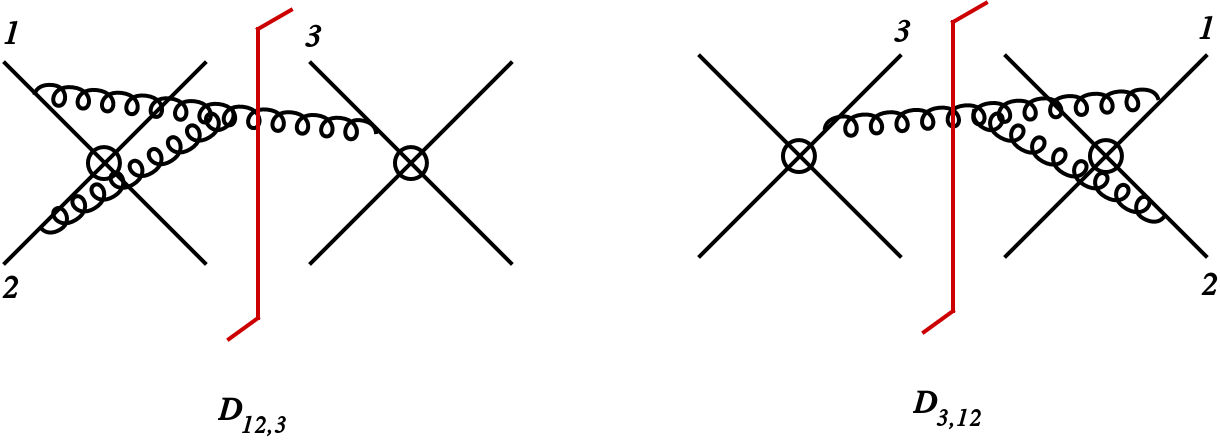
\includegraphics[width=0.60\textwidth]{plots/sf-nnlo-1cut123.png}
  \end{center}
  \caption{Example of the three-Wilson-line, single-cut diagrams that yield
  non-vanishing, purely imaginary result.
  }
  \label{fig:diag123}
\end{figure}

Let us consider a special case of three-Wilson-line diagrams which involve two
massless and one massive particle. Two such diagrams are depicted in
Fig.~\ref{fig:diag123}.
%
Using the notation introduced above, we can write expressions corresponding to
those two diagrams as
%
\begin{align}
  D_{12,3} & = i f^{abc}\, T_3^a T_1^b T_2^c\, 
             \left(e_1^\mu-e_2^\mu\right) e_3^\mu\, g_{12}^{(1)}\,,
  \\[0.5em]
  D_{3,12} & = -i f^{abc}\, T_3^a T_1^b T_2^c\, 
             \left(e_1^\mu-e_2^\mu\right) e_3^\mu\, g_{12}^{(1)\,*}\,.
\end{align}
%
Hence, their sum reads
%
\begin{equation}
  D_{12,3}  + D_{3,12}  = i f^{abc}\, T_3^a T_1^b T_2^c\, 
                          \left(e_1^\mu-e_2^\mu\right) e_3^\mu\,
	                  \left(g_{12}^{(1)}-g_{12}^{(1)\,*}\right)\,.
  %\label{eq:}
\end{equation}

We see that the result is purely imaginary and that, contrary to the case of
double-cut diagrams, it does not vanish as, here, the
antisymmetry of the colour factor under the exchange $1 \leftrightarrow 2$ is
compensated by the antisymmetry of the kinematic part.

We note that our case is different from the one of Ref.~\cite{Becher:2009qa},
which considers infrared singularities of QCD amplitudes and where it is
argued that all three-particle structures with two massless and one massive
Wilson lines must vanish. The latter happens because Ref.~\cite{Becher:2009qa}
discusses amplitudes, \ie objects in which all Wilson lines originate from the
same vertex and all soft gluons are virtual. On the contrary, in our real-virtual
diagrams, the Wilson lines meet at two vertices and one gluon is cut.

To understand better why the contribution from the diagrams of
Fig.~\ref{fig:diag123} does not vanish, it is useful to perform an analysis
similar to the one of Ref.~\cite{Aybat:2006wq}. For that purpose, we use the
soft current for massless particles with momenta $p_{1,2} = (1,0,0,\pm 1)$,
which reads~\cite{Catani:2000pi}
%
\begin{align}
  J_{2P}^{a(1)}(p_1,p_2;p, \epsilon) & = 
  -\frac{1}{16\pi^2}  i f_{abc} T_1^b T_2^c\, \epsilon_\mu(p)
  \left(\frac{p_1^\mu}{p_1\cdot p}- \frac{p_2^\mu}{p_2\cdot p}\right)
  \nonumber \\[0.5em]
  & \quad \quad \times
  \left(\frac{4\pi p_1\cdot p_2}{2\, p_1 \cdot p\ p_2 \cdot p\, e^{-i\pi}}
  \right)^\epsilon
  \frac{1}{\epsilon^2}
  \frac{\Gamma^3(1-\epsilon)\Gamma^2(1+\epsilon)}{\Gamma(1-2\epsilon)}\,.
\end{align}
%
Embedding the above in the integral over $p$ gives
%
\begin{align}
  D_{12,3} & \propto i f_{abc} T_3^a T_1^b T_2^c\,
  \frac{1}{\epsilon^2}\,
  \frac{\Gamma^3(1-\epsilon)\Gamma^2(1+\epsilon)}{\Gamma(1-2\epsilon)}
  \nonumber \\
  & \times
  \int d^d p\,
  \frac{\delta^+(p^2)\delta^{(d-2)}(p_\perp-1)}
       {p_+ p_{3-}+p_- p_{3+}-p_\perp \cdot p_{3\perp}}\,
  \frac{1}{p_+^\alpha}
  \left(\frac{p_{3+}}{p_+}- \frac{p_{3-}}{p_-}\right)
  \left(\frac{4\pi}{p_+\, p_-\, e^{-i\pi}}
  \right)^\epsilon.
\end{align}
%
Let us now apply the change of variables, motivated by Ref.~\cite{Aybat:2006wq}
%
\begin{equation}
  (p_+,p_-,p_\perp) \to (\xi p_-,\xi^{-1} p_+,p_\perp)
  \qquad
  \text{with} 
  \quad
  \xi = p_{3+}/p_{3-}\,.
  \quad
  \label{eq:xiscaling}
\end{equation}
%
Our integral becomes
%
\begin{align}
  D_{12,3} (\alpha) & \propto i f_{abc}  T_3^a T_1^b T_2^c \,
  \frac{1}{\epsilon^2}\,
  \frac{\Gamma^3(1-\epsilon)\Gamma^2(1+\epsilon)}{\Gamma(1-2\epsilon)}
  \nonumber \\
  & \times
  \int d^d p\, 
  \frac{\delta^+(p^2)\delta^{(d-2)}(p_\perp-1)}
       {p_+ p_{3-}+p_- p_{3+}-p_\perp \cdot
  p_{3\perp}}
  \xi^{-\alpha}\frac{1}{p_-^\alpha}
  \left(\frac{p_{3-}}{p_-} - \frac{p_{3+}}{p_+}\right)
  \left(\frac{4\pi}{p_+\, p_-\, e^{-i\pi}}
  \right)^\epsilon
  \nonumber \\
  & = - \xi^{-\alpha} D_{12,3}(-\alpha)\,.
\end{align}
%
Hence, we see that the above integral would exhibit scaling w.r.t. $\xi$, and
vanish, if only there was no $\alpha$ regulator. However, without the regulator,
the integral is divergent. Hence, we conclude that the contribution from
tree-particle graphs with two massless and one massive Wilson lines does not
vanish.

This result only affects the imaginary part of the soft function. The
tree-particle graphs of the type of 123 do not contribute to the real part 
as there will always be a complex-conjugate diagram with opposite
sign due to colour operator.

The above conclusion does not invalidate the analysis of
Ref.~\cite{Aybat:2006wq}, where it is claimed that the massless-massless-massive
diagrams vanish because of the scaling property~(\ref{eq:xiscaling}). The key
difference between our case and the one discussed there is that, in
Ref.~\cite{Aybat:2006wq}, purely virtual diagrams are considered. In those
diagrams, rapidity divergences are regulated by dimensional
regularization~\cite{Becher:2011dz}.  Hence, no $\alpha$ regulator is required
and the $\xi$ scaling of Eq.~(\ref{eq:xiscaling}) holds.

The key element of our calculation, which prevents the diagram 123 from
vanishing, is the transverse delta function. As explained in
Ref.~\cite{Becher:2011dz} without this function, integration over the
transverse momentum provides a factor $k_-^{-\epsilon}$ which regularizes
rapidity divergences, hence there is no need for the regulator $\alpha$. 
%
However, when the transverse delta is present, it fixes $q_\perp$ to some
external value and the integration over $q_\perp$ does not provide a regulator
of light-cone singularities. Hence, we need to introduce the analytic
regulator~$\alpha$.

%-----------------------------------------------------------------------------
\subsubsection{Method of integration}

To evaluate the integrals in Eq.~(\ref{eq:S1cut-main}) we proceed through the
following set of steps. W start from integration over the $p_T$ and $p_-$
components, which is straightforward as, in the process, we use the two delta
functions $\delta(p^2)$ and $\delta(p_T-1)$. Then, we are left with a nontrivial
integration over $p_+$ and  $\cos \phi$ , where $\phi$ is the azimuthal angle
between $v_{3\perp}$ and $p_\perp$. The remaining angular variables do not
appear in the integrand and they only produce a surface term.

To deal with the nontrivial 2-dimensional integrals, we remap the variables
$p_+$ and $\phi$ to a unit hypercube
%
\begin{equation}
  p_+ = \frac{x}{1-x},
  \qquad \qquad
  \cos \phi = 1- 2 \cos^2\frac{\pi y}{2}\,.
  %\label{eq:}
\end{equation}
%
The second transformation is introduced for efficiency reasons as it eliminates
integrable singularity in the azimuthal integration. The first transformation
compactifies the plus component of the gluon momentum. This is useful as our
integrals are in general divergent when integrated over $p_+$. The
divergence comes from rapidity singularities and that is why we have introduced
the analytic regulator in Eq.~(\ref{eq:S1cut-main}).
%
To perform the integral over $x$, we use the Laurent expansion
%
\begin{equation}
  \frac{1}{x^{1+a\alpha}} = -\frac{1}{a\alpha} \delta(x) + \left[
    \frac{1}{x^{1+a\alpha}} \right]_+ \; ,
  \quad
  \text{where}
  \quad
  \int_0^1\!\! dx \, \left[ \frac{1}{x^{1+a\alpha}} \right]_+\!\! f(x) =
  \int_0^1\!\! dx \, \frac{f(x)-f(0)}{x^{1+a\alpha}} \; ,
\end{equation}
%
which makes the divergences explicit by turning them in $\alpha$ poles. All
the coefficients of $\alpha$ expansion are finite and take forms of one and
two-dimensional integrals which we perform numerically with help of the {\tt
Cuba} package~\cite{Hahn:2004fe, Hahn:2014fua}. 
%
The integration is fast, hence, we are able to achieve arbitrary accuracy.


%-----------------------------------------------------------------------------
\subsection{Sector decomposition approach and real-real diagrams}
\label{sec:secdec}

The double-cut integrals take the following form
%
\begin{equation}
  \tilde I = 
  \int \frac{d^d k}{(2\pi)^{d-1}}\, \frac{d^d l}{(2\pi)^{d-1}}\, 
  \frac{\delta^+(k^2) \delta^+(l^2)\,
  \delta(|k_\perp+l_\perp|-1)}
  {(n\cdot k)^{\alpha} (n\cdot l)^\alpha}
  \times \gdp\,.
  \label{eq:int2cutgen}
\end{equation}
%
Two issues arise when one attempts to evaluate them. First of all, 
they are divergent when integrated over a subset of variables, and the pattern
of divergencies is complex, with many overlapping singularities. Secondly, the
remaining part of the integration, where divergencies do not appear, consists of
complicated azimuthal integrals and care is needed to perform them efficiently.

Because of these two separate challenges, it is convenient to factorize the
graph-dependent part as
%
\begin{align}
  \gdp & = \underbrace{\left(\gdp\vert_{\beta_t=0}\right)}_\text{boundary part}
  \underbrace{\left(\frac{\gdp}{\gdp\vert_{\beta_t=0}}\right)}_\text{weight}
  \equiv \calI(n_i, k, l)\, \calW(n_i, k, l)\,.
\end{align}
%
For any graph, the boundary part is not only independent of $\beta_t$ but also
of all the angles except the angle between transverse components of gluons
$d$-momenta $\theta_1 = \sphericalangle(k_\perp, l_\perp)$. In other words, all
divergences are present already in the boundary integrals and the remaining
integration over the  angular variables which appear in the weight is finite.

Our strategy of evaluating the double-cut integrals will therefore consist of
two elements: (i) use of sector decomposition to disentangle overlapping
singularities and cast them into a set of $\alpha$ and $\epsilon$ poles, (ii)
supplementing the sector-decomposed integrals with carefully parameterized
weights and integrating them numerically with {\tt Cuba}.

%-----------------------------------------------------------------------------
\subsubsection{Integration of the on-shell and transverse delta functions}

The momenta of the heavy quarks can be written using the following
parametrization
%
\begin{align}
  \tilde v_3 & = (1, \beta_t \sin \theta\, \hat v_{3\perp}, \beta_t \cos \theta)\,, \\
  \tilde v_4 & = (1, -\beta_t \sin \theta\, \hat v_{3\perp}, -\beta_t \cos \theta) 
               = (1,-\vec v_3)\,,
\end{align}
where $\hat v_{3\perp}$ is a unit vector in $d-2$-dimensional space, \cf
Eq.~(\ref{eq:kparam}).

As discussed in Section~\ref{sec:intsym}, the integrand in
Eq.~(\ref{eq:int2cutgen}) can only depend on the scalar products between
$k_\perp,l_\perp$ and $v_{3\perp}$. Due to rotational invariance of these 
scalar products, one can always change the frame in the transverse space such
that
%
\begin{subequations}
  \begin{align}
    k_\perp & = |k_\perp|\, (1,0, 0, \vec{0}_{d-5}),\\
    l_\perp & = |l_\perp|\, (\cos\theta_1,\sin\theta_1 , 0, \vec{0}_{d-5}),
    \label{eq:theta1} \\
    v_{3\perp} & = |v_{3\perp}|\, (\cos\phi_1,\sin\phi_1\cos\phi_2, 
                         \sin\phi_1\sin\phi_2,\vec{0}_{d-5}).
  \end{align}
  \label{eq:klv3param}
\end{subequations}

Since the momenta of the incoming particles are light-like and $v_{4\perp} =
-v_{3\perp}$, the soft function integrals can only depend on $v_{3\perp}^2$.
Therefore, nothing is sensitive to the position of the versor $\hat v_{3\perp}$.
Hence, the integral~(\ref{eq:int2cutgen}) can be written as
%
\begin{equation}
  \tilde I = 
  \frac{1}{S_{d-3}}
  \int d\Omega_{d-3} (\hat v_{3\perp})
  \int \frac{d^d k}{(2\pi)^{d-1}}\, \frac{d^d l}{(2\pi)^{d-1}}\, 
  \frac{\delta^+(k^2) \delta^+(l^2)\,
  \delta(|k_\perp+l_\perp|-1)}
  {(n\cdot k)^{\alpha} (n\cdot l)^\alpha}
  \times \gdp\,,
\end{equation}
%
where the surface of unit-sphere, $S_{d-3}$, is given by Eq.~(\ref{eq:Sd}),
and the differential measures  read
%
\begin{subequations}
  \label{eq:klv3-measures}
  \begin{align}
   d^{d}k_\perp & =  dk_+ dk_- d k_\perp  k_\perp^{d-3}\,
   d\Omega(\chi_1,\chi_2, \dots, \chi_{d-3}),
   \\[0.5em]
   d^{d} l_\perp & =  dl_+ dl_- d l_\perp  l_\perp^{d-3}\,
   d\Omega(\theta_1,\theta_2, \dots, \theta_{d-3}),
   \\[0.5em]
   d\Omega_{d-3} (\hat v_{3\perp}) & =  
   d\Omega(\phi_1,\phi_2, \dots, \phi_{d-3})\,.
  \end{align}
\end{subequations}
%
Because we use the parametrization~(\ref{eq:klv3param}),
all the angles except $\theta_1$, $\phi_1$  and $\phi_2$ can be
integrated trivially. 
%
Let us now replace the angle between the transverse components of the two
gluons' momenta, $\theta_1$, by
%
\begin{equation}
  \eta = \frac{1-\cos\theta_1}{2}\,.
  \label{eq:eta-def}
\end{equation}
%
Then, the whole measure takes the form
%
% NOTE
% my paper notes
%
\begin{align}
  d\Omega_{d-3} (\hat v_{3\perp})\,
  d^d k\, d^d l & =
  \\
  &
  \hspace{-50pt}
  4^{-\epsilon}
  S_{1-2\epsilon}\,
  S_{-2\epsilon}\,
  k_T^{1-2\epsilon} \,
  l_T^{1-2\epsilon} 
  \big((1-\eta)\eta \big)^{-\frac12-\epsilon}
  dk_+ dk_- dl_+ dl_-
  d k_T\, 
  d l_T\,
  d\eta\,
  d\Omega(\phi_1, \phi_2, \ldots, \phi_{d-3})\,,
  \nonumber
  %\label{eq:}
\end{align}
%
where we used Eqs.~(\ref{eq:rot-inv-measure}), (\ref{eq:klv3-measures}) and
(\ref{eq:eta-def}).
%
After performing the graph-independent integrations over $k_-$, $l_-$ and
$\eta$, where the last quantity gets fixed to
%
\begin{equation}
  \eta = \frac{k_T^2 + l_T^2+ 2 k_T l_T -1}{4 k_T l_T}\,,
  %\label{eq:}
\end{equation}
the integral~(\ref{eq:int2cutgen}) turns into
%
\begin{align}
  \tilde I & =
  \int dk_+\, dl_+\, dk_T\, dl_T\, 
  d\Omega(\phi_1, \phi_2, \ldots, \phi_{d-3})\,
  k_+^{-\alpha}\, l_+^{-\alpha} k_T^{1-2\epsilon} l_T^{1-2\epsilon} \,
  \nonumber \\ &
  \times\,
  \Big\{\big[1-(k_T-l_T)^2\big]\big[1-(k_T+l_T)^2\big]
  \Big\}^{-\frac12-\epsilon}
  {\cal I}(n_i, k_+, l_+, k_T, l_T)\,
  {\cal W}(n_i, k_+, l_+, k_T, l_T, \phi_1, \phi_2, \beta_t)\,,
  \label{eq:S2cutgen-deltaint}
\end{align}
%
and the delta functions generate the following relations
%
\begin{equation}
  k_- = \frac{k_T^2}{k_+}\,, \qquad \qquad
  l_- = \frac{l_T^2}{l_+},
  \label{eq:pmrelations}
\end{equation}
%
and
\begin{equation}
  | k_T - l_T | \leq 1
  \qquad \land \qquad
   k_T + l_T  \geq 1\,.
  \label{eq:kTlT-region}
\end{equation}
%
The last pair of inequalities defines the integration region in the $(k_T, l_T)$
plane,  which is depicted in Fig.~\ref{fig:trans-regions}~(left).  The
first inequality corresponds to the two (red) solid lines, while the second
inequality corresponds to the (blue) dotted line.

\begin{figure}[t]
  \begin{center}
    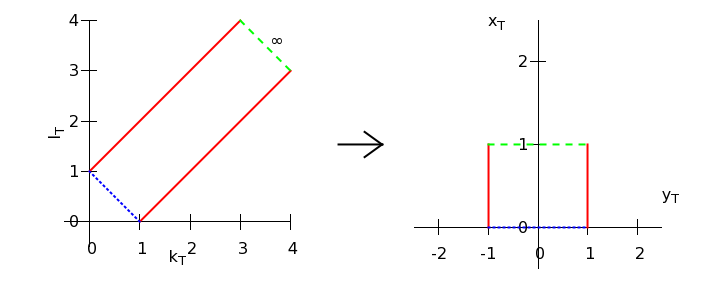
\includegraphics[width=0.99\textwidth]{plots/transverse-phase-space.png}
  \end{center}
  \caption{
  The integration region in the transverse coordinates before (left) and
  after (right) the transformation of variables from Step 1 discussed in
  Section~\ref{sec:mapping}.
  }
  \label{fig:trans-regions}
\end{figure}

%-----------------------------------------------------------------------------
\subsubsection{Divergencies}

The non-integrable divergences of the integral~(\ref{eq:S2cutgen-deltaint}) come
from the graph-dependent part. Since the weight is finite, the divergences
are fully determined by the boundary integrand ${\cal I}(n_i, k_+, l_+, k_T,
l_T)$.
%
Hence, each integral can in principle diverge due to integration over the four
independent variables:  $k_+, l_+, k_T$ and $l_T$, and some of the limits are
coupled due to the constraint of Eq.~(\ref{eq:kTlT-region}).
%
The singularities of the integral $\tilde I$ correspond to vanishing of the
propagators in $\cal I$, and this can happen in the following situations.

%------------------------------------
\subsubsection*{Propagators of the incoming particles}

The incoming-particle propagators, $n\cdot k$, $\nbar\cdot k$, $n\cdot l$ and
$\nbar\cdot l$, produce divergencies in the limits in which the plus or minus
components of the momenta of gluons tend to zero or infinity. This occurs
in three regions of gluons' momenta
%
\begin{itemize}
  %\setlength\itemsep{1.2em}
  \item
  Rapidity region, where the momenta scale as 
  $(\lambda^{\pm 1},\lambda^{\mp 1},1)$. 
  In terms of the independent variables, the rapidity divergencies occur when
  \begin{equation}
    k_+ \to 0      \qquad \text{or} \qquad
    k_+ \to \infty \qquad \text{or} \qquad
    l_+ \to 0      \qquad \text{or} \qquad
    l_+ \to \infty\,.
  \end{equation}
  \item
  Soft region, with the momenta scaling like
  $(\lambda, \lambda, \lambda)$. This corresponds to either
  %
  \begin{equation}
    k_+ \to 0,\ k_T \to 0 \qquad \text{or} \qquad
    l_+ \to 0,\ l_T \to 0\,.
    \label{eq:softlimit-var}
  \end{equation}
  % 
  We note that, when one gluon becomes
  soft, transverse momentum of the other gluon tends to one due to the
  constraint~(\ref{eq:kTlT-region}).
  \item
  Collinear region, characterized by the scaling
  $(1,\lambda^2,\lambda)$. In terms of the independent variables, the collinear
  singularity occurs when
  %
  \begin{equation}
    k_T \to 0 \qquad \text{or} \qquad
    l_T \to 0\,.
    %\label{eq:}
  \end{equation}
  %
  Similarly to the case of the soft limit, because of the
  constraint~(\ref{eq:kTlT-region}), vanishing of the transverse momentum of one
  gluon requires that the transverse momentum of the other gluon tends to
  one, \ie the second gluon cannot be soft or collinear to the incoming parton.
  %
  The reason why the collinear limit leads to vanishing of one of the
  incoming-particle propagators is because of the
  relation~(\ref{eq:pmrelations}).
\end{itemize}

%------------------------------------
\subsubsection*{Propagators of the outgoing particles}

The propagators involving top or anti-top quark, $v_3\cdot k$, $v_4\cdot k$,
$v_3 \cdot l$ and $v_4\cdot l$, vanish only in the soft region.  In terms of the
independent variables, the latter corresponds to the limits given in
Eq.~(\ref{eq:softlimit-var}) above.  

To see that the massive-particle propagators can produce divergencies only in
the soft region, let us use the parametrization of Eqs.~(\ref{eq:klv3param})
and the relation (\ref{eq:pmrelations}). Together they give
%
\begin{align}
  v_{3} \cdot k & =
  \frac{v_{3+} k_-}{2} + \frac{v_{3-} k_+}{2} - v_{3\perp} \cdot k_\perp
  \nonumber \\[0.2em]
  & =
  \frac{1+\beta_t \cos\theta}{2}\, \frac{k_T^2}{k+} + 
  \frac{1-\beta_t \cos\theta}{2}\, k_+ - 
  \beta_t \sin\theta\, k_T\,.
  \label{eq:v3knonvanish}
\end{align}
%
Since $\beta_t \leq \sqrt{1-m_t^2/\shat} < 1$ and $-1 \leq \cos\theta \leq 1$, the
coefficients in front of the components of gluon's $d$-momentum in the first two
terms in Eq.~(\ref{eq:v3knonvanish}) can never vanish. The collinear region
corresponds to $k_T \to $ and finite $k_+$, and we see that the propagator
stays finite in this limit. Similarly, the propagator does not vanish when $k_+
\to 0$ or $k_+ \to \infty$, while $k_T \neq 0$, which is the region of
small/large rapidities of the gluon.  Hence, the only way to make the above
propagator vanish is to send $k_+$ and $k_T$ to zero simultaneously, 
and this corresponds to the soft limit.
%
The above proof can be repeated for the other propagators of the outgoing
particles.


%------------------------------------
\subsubsection*{Exact gluon propagator}

Double-cut diagrams with the triple gluon vertex contain the propagator $(k + l)^2$
in which the momenta of the gluons are commensurate.  After the integration over
$k_-$, $l_-$ and $\eta$ is performed, this exact propagator
reads
%
% NOTE
% my paper notes
%
\begin{equation}
  (k+l)^2  = 2\,k\cdot l  =   
  -1 + 
  \frac{k^+ + l^+}{k^+}\, k_\perp^2  + 
  \frac{k^+ + l^+}{l^+}\, l_\perp^2\,.
  %\label{eq:}
\end{equation}
%
Within the domain of integration defined in
Fig.~\ref{fig:trans-regions} (left), the above propagator vanishes when
%
\begin{equation}
  k_T \to \frac{k^+}{k^+ + l^+} 
  \qquad \text{and} \qquad
  l_T \to \frac{l^+}{k^+ + l^+}\,.
  \label{eq:colllimit}
\end{equation}
%
This limit corresponds to the two gluons with momenta $k$ and $l$ becoming
collinear. 
%
Note that, due to condition~(\ref{eq:kTlT-region}), only one of the two gluons
can have vanishing transverse momentum.
%
One notices that the limit (\ref{eq:colllimit}) is different with respect to the
cases discusses earlier. While the divergencies of the eikonal propagators
happen only at the edges of the integration domain, \ie $0$ or $\infty$
(endpoint singularities), the exact propagator vanishes inside the integration
region, on the manifold defined by Eq.~(\ref{eq:colllimit}).


%-----------------------------------------------------------------------------
\subsubsection{Mapping procedure}
\label{sec:mapping}

We would like to transform the integration region in the $(\kp, \lp, k_T, l_T)$
space into a unit hyper-cube in the space of variables $\{x_i\}$, and, if
necessary, split it such that each of the resulting integrals $\int \prod_i d
x_i f(\{x_i\})$ has singularities only when one or more variables $x_i \to 0$.
%
We achieve the above in the following four steps:
 

%------------------------------------
\subsubsection*{Step 1}

The transverse variables $(k_T, l_T)$ are transformed to new variables 
$(x_T, y_T)$ with the replacements
%
\begin{equation}
  k_T = \frac{1+y_T-x_T y_T}{2(1-x_T)}\,,
  \qquad \qquad
  l_T = \frac{1-y_T+x_T y_T}{2(1-x_T)}\,,
  %\label{eq:}
\end{equation}
%
and the inverse transformation reads
\begin{equation}
  x_T = 1-\frac{1}{k_T+l_T}\,,
  \qquad \qquad
  y_T = k_T-l_T\,.
  %\label{eq:}
\end{equation}
%
This results in change of the integration region from the one shown in
Fig.~\ref{fig:trans-regions}~(left) to that of
Fig.~\ref{fig:trans-regions}~(right). The latter corresponds to
%
\begin{equation}
  0 \leq x_T \leq 1
  \qquad \land \qquad
  -1 \leq y_T \leq 1\,.
  %\label{eq:}
\end{equation}
%
The collinear divergences now occur in the limits
\begin{eqnarray}
  x_T \to 0,\, y_T \to -1 \qquad \text{or} \qquad
  x_T \to 0,\, y_T \to 1\,, 
  %\label{eq:}
\end{eqnarray}
and the soft divergences correspond to
\begin{eqnarray}
  k_+ \to 0,\,  x_T \to 0,\, y_T \to -1 \qquad \text{or} \qquad
  l_+ \to 0,\,  x_T \to 0,\, y_T \to 1\,. 
  %\label{eq:}
\end{eqnarray}
%
The limit of two gluons becoming collinear, Eq.~(\ref{eq:colllimit}), in the new
variables happens when
%
% NOTES
% short-derivations.nb
%
\begin{equation}
  x_T \to 0,\ y_T \to \displaystyle \frac{\kp-\lp}{\kp+\lp}\,.
  \label{eq:manifoldsing1}
\end{equation}
%
The last divergence occurs on a manifold inside the integration region as
depicted in Fig.~\ref{fig:yTmanifold}.

\begin{figure}[t]
  \begin{center}
    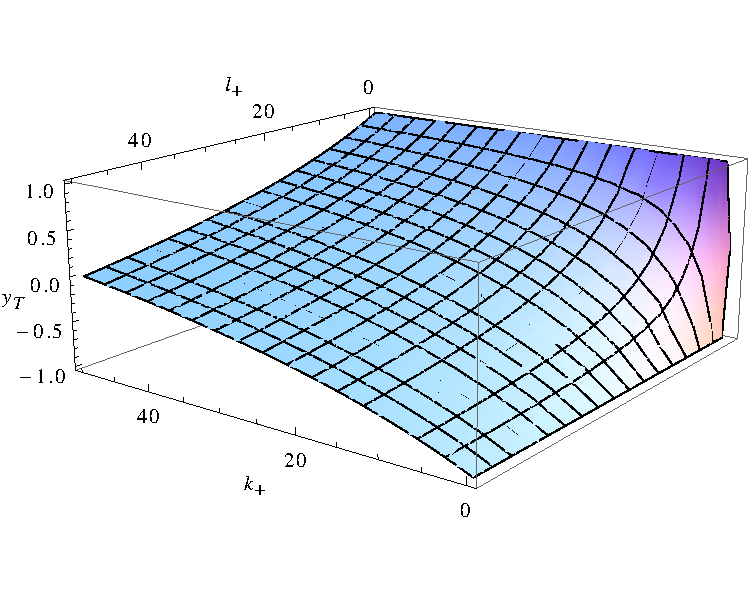
\includegraphics[width=0.49\textwidth]{plots/yTmanifold.pdf}
  \end{center}
  \caption{
  Manifold where the double-cut integrals with triple-gluon vertex become
  divergent. It corresponds to the limit of the two gluons $k$ and $l$ becoming
  collinear to each other.
  }
  \label{fig:yTmanifold}
\end{figure}

%------------------------------------
\subsubsection*{Step 2}

In order to transform the manifold singularity (\ref{eq:manifoldsing1}) into
an endpoint singularity, we split the integration region in the variable $y_T$
precisely on the manifold of Fig.~\ref{fig:yTmanifold}
%
% NOTES
% short-derivations.nb
%
\begin{eqnarray}
  I & =  & 
  \int_0^\infty\!\!\! d\kp
  \int_0^\infty\!\!\! d\lp
  \int_0^1\!\!\! d x_T
  \int_{-1}^1\!\!\! d y_T\
  \bar I(\kp, \lp, x_T, y_T)
  \nonumber \\
  & = &
  \int  d\kp d\lp d x_T
  \int_{-1}^{c(\kp, \lp)}\!\!\! d y_T\
  \bar I(\kp, \lp, x_T, y_T)
  +
  \int  d\kp d\lp d x_T
  \int_{c(\kp, \lp)}^{1}\!\!\! d y_T\
  \bar I(\kp, \lp, x_T, y_T)
  \nonumber \\
  & \equiv &
  I_d + I_u\,,
  %\label{eq:}
\end{eqnarray}
%
where
%
\begin{equation}
  c(\kp, \lp) = \frac{\kp-\lp}{\kp+\lp}\,.
  %\label{eq:}
\end{equation}
%
Now, we use two different parametrizations
%
\begin{equation}
  y_T = \frac{\kp-\lp + 2 \lp \bar y_T}{\kp+\lp}\,,
  \qquad 
  \bar y_T = \frac{y_T-c(\kp,\lp)}{1-c(\kp,\lp)}
           = \frac{k_+ (-1 + y_T) + l_+ (1+ y_T)}{2 l_+}
  \qquad 
  \text{for}\quad I_u\,,
  %\label{eq:}
\end{equation}
%
and
%
\begin{equation}
  y_T = \frac{\kp-\lp - 2 \kp \bar y_T}{\kp+\lp}\,,
  \qquad
  \bar y_T = \frac{y_T-c(\kp,\lp)}{1-c(\kp,\lp)}
           = \frac{k_+ (1 - y_T) - l_+ (1+ y_T)}{2 k_+}
  \qquad
  \text{for}\quad I_d\,.
  %\label{eq:}
\end{equation}
%
Hence, we obtain
%
\begin{subequations}
  %\label{eq:}
  \begin{align}
    I_d  & =  
     \int_0^\infty\!\!\! d\kp
     \int_0^\infty\!\!\! d\lp
     \int_0^1\!\!\! d x_T
     \int_{0}^1\!\!\! d \bar y_T\
     \bar I_u(\kp, \lp, x_T, \bar y_T)\,,
     \\[0.5em]
    I_u  & =  
     \int_0^\infty\!\!\! d\kp
     \int_0^\infty\!\!\! d\lp
     \int_0^1\!\!\! d x_T
     \int_{0}^1\!\!\! d \bar y_T\
     \bar I_d(\kp, \lp, x_T, \bar y_T)\,.
  \end{align}
  \label{eq:IuIdstep2}
\end{subequations}
%
With the above changes, the soft singularities happen at
%
\begin{equation}
  k_+ \to 0,\ x_T \to 0
  \qquad \text{or} \qquad
  l_+ \to 0,\ x_T \to 0\,,
  %\label{eq:}
\end{equation}
in both integrals, $I_u$ and $I_d$, and for any value of $\bar y_T$. 
%
The case in which a gluon is collinear to the incoming parton corresponds to
%
\begin{equation}
  \bar y_T \to 1\,,
  \label{eq:yTbarlimit}
\end{equation}
for both integrals. We note that in the above limit, for $I_u$, it is the gluon
with momentum $l$ that becomes collinear, whereas, for $I_d$, the limit
(\ref{eq:yTbarlimit})  corresponds to the gluon with momentum $k$ being
collinear to the beam.

Finally, the limit of two gluons becoming collinear to each other,
Eq.~(\ref{eq:colllimit}), in the new variables corresponds to 
\begin{equation}
  x_T \to 0,\ \bar y_T \to 0\,,
  %\label{eq:}
\end{equation}
%
for both $I_u$ and $I_d$.


%------------------------------------
\subsubsection*{Step 3}

We see that  the integrals (\ref{eq:IuIdstep2}) can be divergent at both ends in
the variable $\bar y_T$.
%
In order to move all singularities to the limit $x_i \to 0$, we split $I_u$ and
$I_d$ at $\bar y_T = \frac12$
%
\begin{equation}
 I_{\{u,d\}} = \int_0^1 d \bar y_T\, \tilde I_{\{u,d\}} =
 \int_0^\frac12 d \bar y_T\, \tilde I_{\{u,d\}} +
 \int_\frac12^1 d \bar y_T\, \tilde I_{\{u,d\}} \equiv 
 I_{\{u,d\}0} + I_{\{u,d\}1}\,.
  %\label{eq:}
\end{equation}
%
Then, we apply the following transformations
%
\begin{equation}
  \tilde y_T = 2(1-\bar y_T)\,,
  \qquad \qquad
  \bar y_T = 1-\frac{\tilde y_T}{2}\,,
  \qquad 
  \text{for}\quad I_{\{u,d\}1}\,,
  %\label{eq:}
\end{equation}
%
and
%
\begin{equation}
  \tilde y_T = 2 \bar y_T\,,
  \qquad \qquad
  \bar y_T = \frac{\tilde y_T}{2}\,,
  \qquad 
  \text{for}\quad I_{\{u, d\}0}\,.
  %\label{eq:}
\end{equation}
%
At this point, we have the following singularities:
%
\begin{equation}
  {\renewcommand{\arraystretch}{1.5}% 
  \begin{array}{c@{\qquad \quad}c@{\qquad \quad}l}
   \text{soft}     &  
   k_+ \to 0,\  x_T \to 0 \quad \text{or} \quad l_+ \to 0,\  x_T \to 0 &
   I_{u0}, I_{u1}, I_{d0}, I_{d1}\,,              \\
   \text{collinear} & 
   x_T \to 0,\ \tilde y_T \to 0 & 
   I_{u1}, I_{d1}\,, \\
   k \parallel l & 
   x_T \to 0,\ \tilde y_T \to 0 & 
   I_{u0}, I_{d0}\,. 
  \end{array}
  }
\end{equation}

%------------------------------------
\subsubsection*{Step 4}

In the last step, we compress the ranges of the $\kp$ and $\lp$ integrals by the
transformation
%
\begin{equation}
  \kp = \frac{x}{1-x}\,, 
  \qquad \qquad
  \lp = \frac{y}{1-y}\,, 
\end{equation}
%
whose inverse reads
\begin{equation}
  x = \frac{\kp}{1+\kp}\,, 
  \qquad \qquad
  y = \frac{\lp}{1+\lp}\,.
\end{equation}
%
Hence, finally, our integral is a sum of four contributions
%
\begin{equation}
  I = I_{d0} + I_{d1} + I_{u0} + I_{u1}\,.
  %\label{eq:}
\end{equation}

%-----------------------------------------------------------------------------
\subsubsection{Integrating the weight}

As a final step, we integrate the weight over the azimuthal angles of  $v_3$:
$\phi_1$ and $\phi_2$. In order to map the angular variables into a unit
hypercube, we first write the integration measure as

\begin{align}
  \int_{S_1^{d-3}}\!\!\! d\Omega(\phi_1,\phi_2,\ldots,\phi_{d-3}) 
  & =
  \int_{S_1^{1-2\epsilon}}\!\!\!
  d\Omega(\phi_1,\phi_2,\ldots,\phi_{1-2\epsilon}) 
  \nonumber \\
  & =
  \int_{-1}^1 d\cos\phi_1 \sin^{-1-2\epsilon}\phi_1
  \int_{S_1^{-2\epsilon}}\!\!\! d\Omega(\phi_2,\ldots,\phi_{1-2\epsilon})\,.
  %\label{eq:}
\end{align}
%
Then, we represent the remaining measure as~\cite{Czakon:2014oma}
%
% NOTE
% eqs. (87), (89) there
%
\begin{align}
  \int_{S_1^{-2\epsilon}} {d}{\Omega}(\phi_2, \ldots, \phi_{1-2\epsilon}) & =
  \frac{(4\pi)^{-\epsilon}\Gamma(1-\epsilon)}{\Gamma(1-2\epsilon)} 
  \\
  &
  \hspace{-70pt}
  \times \int_{-1}^{+1} {d}\cos\phi_2 \left( \delta(1-\cos\phi_2)
  + \delta(1 + \cos\phi_2) - 2 \epsilon \, \frac{4^\epsilon
    \Gamma(1-2\epsilon)}{\Gamma^2(1-\epsilon)} \left[
    \frac{1}{(1-\cos^2\phi_2)^{1+\epsilon}} \right]_+\right)\,,
  \nonumber
\end{align}
%
where we used the fact that our integrand is independent of the angles $\phi_3,
\ldots, \phi_{1-2\epsilon}$. The plus distribution is defined as

\begin{align}
  \int_{-1}^{+1} {d}\cos\rho \left[
  \frac{1}{(1-\cos^2\rho)^\alpha} \right]_+ f(\cos\rho) 
  & 
  \\[0.5em]
  & \hspace{-80pt} =
  \int_{-1}^{0} {d}\cos\rho \,
  \frac{f(\cos\rho)-f(-1)}{(1-\cos^2\rho)^\alpha} 
  + \int_{0}^{+1} {d}\cos\rho \,
  \frac{f(\cos\rho)-f(+1)}{(1-\cos^2\rho)^\alpha}
  \; .
  \nonumber
  %\label{eq:}
\end{align}
%
The integral over the weight now reads
%
\begin{align}
  & \frac{1}{S_{1-2\epsilon}}\int_{S_1^{1-2\epsilon}}
  d\Omega (\phi_1,\phi_2,\ldots,\phi_{1-2\epsilon})   
  \calW(\beta_t,\theta,\phi_1,\phi_2)=
  \frac{(4\pi)^{-\epsilon}\Gamma(1-\epsilon)}{\Gamma(1-2\epsilon)}
  \int_{-1}^{1}d\!\cos{\phi_1}\,\sin^{-1-2\epsilon}\phi_1 
  \nonumber \\[0.5em]
  & \times \left[ 
  \int_{0}^{1}d\!\cos{\phi_2} \left( \delta(1-\cos{\phi_2})
  \calW(\beta_t,\theta,\phi_1,0)
  -2\epsilon \frac{4^\epsilon \Gamma(1-2\epsilon)}{\Gamma^2(1-\epsilon)} 
  \frac{\calW(\beta_t,\theta,\phi_1,\phi_2)-
  \calW(\beta_t,\theta,\phi_1,0)}{\left( 1-\cos^2\phi_2\right)^{1+\epsilon}}  \right)
  \right.
  \nonumber \\[0.5em]
  &+ \left.
  \int^{0}_{-1}d\!\cos{\phi_2} \left( \delta(1+\cos{\phi_2})
  \calW(\beta_t,\theta,\phi_1,\pi)
  -2\epsilon \frac{4^\epsilon \Gamma(1-2\epsilon)}{\Gamma^2(1-\epsilon)} 
  \frac{\calW(\beta_t,\theta,\phi_1,\phi_2)-\calW(\beta_t,\theta,
  \phi_1,\pi)}{\left( 1-\cos^2\phi_2\right)^{1+\epsilon}}  \right)
  \right]\,.
\end{align}
%
%
To map this integral to a unit hypercube, we use the following changes 
of variables
%
\begin{equation}
  \cos\phi_1= 1-2 \cos^2(\chi \pi /2) , \qquad 
  \cos\phi_2= 1-\eta_2, \qquad
  \sin^2\phi_2=\eta_2(2-\eta_2)\,,
  %\label{eq:}
\end{equation}
%
in the second 
%
\begin{equation}
  \cos\phi_1= 1-2 \cos^2(\chi \pi /2) , \qquad 
  \cos\phi_2= \eta_2-1, \qquad
   \sin^2\phi_2=\eta_2(2-\eta_2)\,,
  %\label{eq:}
\end{equation}
and the third line, respectively.
%
From these, one gets 
%
\begin{align}
  & \frac{1}{S_{1-2\epsilon}}\int_{S_1^{1-2\epsilon}}
  d\Omega (\phi_1,\phi_2,\ldots,\phi_{1-2\epsilon})   
  \calW(\beta_t,\theta,\phi_1,\phi_2)=
  \calR
  \int_{0}^{1}  d \chi \, \sin^{-2\epsilon}(\pi \chi)
   \nonumber\\
  & \times \left[ 
  \int_{0}^{1}d \eta_2 
  \left( 4^{-\epsilon}
  \delta(1-\cos{\phi_2}) \calW(\beta_t,\theta,\phi_1,0)
  -\frac{\epsilon}{\calR} 
  \frac{\calW(\beta_t,\theta,\phi_1,\phi_2)-\calW(\beta_t,\theta,
  \phi_1,0)}{\left( 1-\cos^2\phi_2\right)^{1+\epsilon}}  \right)
  \right.+\nonumber \\
  &\left.
  \int_{0}^{1}d \eta_2 \left( 
  4^{-\epsilon} \delta(1+\cos{\phi_2}) \calW(\beta_t,\theta,
  \phi_1,\pi)
  -\frac{\epsilon}{\calR} 
  \frac{\calW(\beta_t,\theta,\phi_1,\phi_2)-\calW(\beta_t,\theta,
  \phi_1,\pi)}{\left( 1-\cos^2\phi_2\right)^{1+\epsilon}}  \right) 
  \right]\,,
  \label{eq:v3average}
\end{align}
where we define the prefactor
%
\begin{equation}
  \calR = \frac{\Gamma(1-\epsilon)^2}{2\Gamma(1-2\epsilon)}.
\end{equation}


%-----------------------------------------------------------------------------
\section{NNLO soft function: results}
\label{sec:results}

\begin{figure}[t]
  \begin{center}
    \includegraphics[width=0.99\textwidth]{plots/soft-function-qq-qbub-beta.png}
    %\includegraphics[width=0.99\textwidth]{../../complete/plots/soft-function-qq-qbub-beta.png}
  \end{center}
  \caption{
  Quark bubble contribution to the NNLO soft function in the \qqbar channel.
  The plots correspond to three independent entries of the $2\times 2$ matrix
  determined for the fixed values of $\theta = \pi/4$ and $\LT = 0$.
  %
  We see perfect agreement between RG prediction and the direct calculation
  obtained with two independent methods: differential equations~(DE) and sector
  decomposition~(SD).
  }
  \label{fig:quarkbubbleqq}
\end{figure}

\begin{figure}[!h]
  \begin{center}
    \includegraphics[width=0.99\textwidth]{plots/soft-function-gg-qbub-beta.png}
    %\includegraphics[width=0.99\textwidth]{../../complete/plots/soft-function-gg-qbub-beta.png}
  \end{center}
  \caption{
  Quark bubble contribution to the NNLO soft function in the $gg$ channel.
  The plots correspond to six independent entries of the $3\times 3$ matrix
  determined for the fixed values of $\theta = \pi/4$ and $\LT = 0$.
  %
  We see perfect agreement between RG prediction and the direct calculation
  obtained with two independent methods: differential equations~(DE) and sector
  decomposition~(SD).
  }
  \label{fig:quarkbubblegg}
\end{figure}


The bare NNLO soft function for the top pair production has the following
structure
%
\begin{equation}
  \bfS^{(2)}_\text{bare}(\LT, \beta_t,\theta) =
  \frac{1}{\epsilon^2} \bfS^{(2,-2)}(\LT, \beta_t,\theta) +
  \frac{1}{\epsilon} \bfS^{(2,-1)}(\LT, \beta_t,\theta)
  + \bfS^{(2,0)}(\LT, \beta_t,\theta)\,.
  \label{eq:bareSFNNLOpoles}
\end{equation}
%
Because it encodes single and double-soft limit, it exhibits at most
$1/\epsilon^2$ singularity. However, higher order $\epsilon$ poles, as well as
$\alpha$ poles, appear at intermediate stages of the calculation, but they
cancel in the final combination.

We have checked that, in our calculation, all $\alpha$ poles, including
$\epsilon/\alpha$, as well as $1/\epsilon^4$ vanish within each colour structure
defined in Eq.~(\ref{eq:w1w2def}). As for the $1/\epsilon^3$ pole, it comes out
with a non-zero coefficient in the single-cut and in the double-cut
contributions. The value of the $1/\epsilon^3$ coefficient is however identical,
in those two pieces up to a sign. Hence, in the final combination, this pole
does not appear in our result.
%
We have demonstrated that, when all contributions to the bare NNLO soft
function are included, following Eq.~(\ref{eq:bareSFNNLOdef}) the soft function
indeed shows at most $1/\epsilon^2$ singularity.

As discussed in Section~\ref{sec:renormalization}, the pole part of the soft
function, \ie the functions $S^{(2,-2)}(\LT, \beta_t,\theta)$ and
$S^{(2,-1)}(\LT, \beta_t,\theta)$ defined in Eq.~(\ref{eq:bareSFNNLOpoles}), as
well as the $\LT$-dependent part of the finite contribution, $S^{(0,0)}(\LT,
\beta_t,\theta)$, can be completely determined from the renormalization group. 
%
The only term that has to be obtained through direct calculation is the
$\LT$-independent part of $S^{(2,0)}(\LT, \beta_t,\theta)$. 
%
In spite of the above, it is worth calculating all the terms appearing in
Eq.~(\ref{eq:bareSFNNLOpoles}) and use the
redundant ones for cross checks of our framework against RG prediction.

As much as the comparison of the results from direct calculations to the
prediction of the renormalization group is valuable, it is limited by the fact
that RG misses the constant part of $S^{(2,0)}(\LT, \beta_t,\theta)$. In our
calculation, we are however able to cross-check this missing component as well
since part of our soft function, namely the one corresponding to the bubble and
tadpole diagrams, can be determined with two completely different methods:
differential equations and sector decomposition.


Figs.~\ref{fig:quarkbubbleqq} and \ref{fig:quarkbubblegg} show the results for
the quark bubble part of the soft function, respectively in the \qqbar and the
$gg$ channel, obtained from the renormalization group and from the direct
calculation with differential equations and with sector decomposition. 
%
The quark bubble contribution can be singled out from the RG prediction as it is
proportional to $n_f$.
%
The plots correspond to three independent entries of the $2\times 2$ matrix and
six independent entries of the $3\times 3$ matrix, determined for the fixed
values of $\theta = \pi/4$ and $\LT = 0$, and shown as a function of $\beta_t$.
We see perfect agreement between the two sets of points as well as between the
points and the RG prediction.  The error bars in the result from sector
decomposition come from the uncertainties of numerical integration. 
%
We have performed similar comparison of the results from differential equations
and sector decomposition for the gauge bubble and for the tadpole, in both
channels, each time finding an excellent agreement.

This constitutes a very strong validation of our computational framework. It
tests all the elements of the sector decomposition method and tools, discussed
in Section~\ref{sec:secdec}, up to the finite order in $\epsilon$. Even though
the bubble graphs are easier to solve analytically than the rest of the
double-cut graphs, they pose a serious challenge to the sector decomposition
approach due to non-trivial numerators. Therefore, the comparison shown in
Figs.~\ref{fig:quarkbubbleqq} and \ref{fig:quarkbubblegg} makes up a
highly-nontrivial test of the entire framework used in the calculation of the
NNLO soft function.

\begin{figure}[t]
  \begin{center}
    \includegraphics[width=0.99\textwidth]{plots/soft-function-qq-re-beta.png}
    %\includegraphics[width=0.99\textwidth]{../../complete/plots/soft-function-qq-re-beta.png}
  \end{center}
  \caption{
  Real part of the NNLO soft function in the \qqbar channel.
  The figure shows three independent entries of the $2\times 2$ matrix
  determined for the fixed values of $\theta = \pi/4$ and $\LT = 0$.
  %
  All the points come from our direct calculation at different orders in
  $\epsilon$ expansion. The two results at order $\epsilon^0$ correspond to the
  finite part of the NNLO soft function before and after renormalization.
  %
  The RG predictions for the pole part are shown as
  red~(dashed) and green~(solid) lines.
  %
  The points for order $\epsilon^0$ are connected by straight lines for better
  visibility.
  }
  \label{fig:SFresqqreal}
\end{figure}

\begin{figure}[!t]
  \begin{center}
    \includegraphics[width=0.99\textwidth]{plots/soft-function-gg-re-beta.png}
    %\includegraphics[width=0.99\textwidth]{../../complete/plots/soft-function-gg-re-beta.png}
  \end{center}
  \caption{
  Real part of the NNLO soft function in the $gg$ channel.  The figure shows six
  independent entries of the $3\times 3$ matrix. All details as in
  Fig.~\ref{fig:SFresqqreal}.
  }
  \label{fig:SFresggreal}
\end{figure}

We are now in a position to present the complete NNLO soft function for top
quark pair production at small $q_T$.  The results for the real part of the
independent entries of the matrices in the \qqbar and $gg$ channel, at fixed
values of $\theta = \pi/4$ and $\LT = 0$, are given in
Figs.~\ref{fig:SFresqqreal} and \ref{fig:SFresggreal}, respectively.
%
The points correspond to our direct calculation at orders $1/\epsilon^2$,
$1/\epsilon$ and $\epsilon^0$. 

For the poles, we also show, as lines,
predictions from the renormalization group. We see that the two sets of
predictions agree perfectly.

For the finite term, we show two sets of points: the one
before and the one after renormalization. They differ by a finite function
following the formula~(\ref{eq:renS2}). We notice that the difference is often
substantial.

\begin{figure}[!t]
  \begin{center}
    \includegraphics[width=0.33\textwidth]{plots/soft-function-qq-im-beta.png}
    %\includegraphics[width=0.33\textwidth]{../../complete/plots/soft-function-qq-im-beta.png}
    \hspace{35pt}
    \includegraphics[width=0.33\textwidth]{plots/soft-function-gg-im-beta.png}
    %\includegraphics[width=0.33\textwidth]{../../complete/plots/soft-function-gg-im-beta.png}
  \end{center}
  \caption{
  Imaginary part of the NNLO soft function in the \qqbar channel (left) and in
  the $gg$ channel (right).
  %
  The figures show the only one independent structure in each matrix. All
  details as in Fig.~\ref{fig:SFresqqreal}.
  }
  \label{fig:SFresim}
\end{figure}

As discussed in Section~\ref{sec:realvirt}, due to the real-virtual
contributions, the NNLO soft function contains also an imaginary part.  As
follows from Eqs.~(\ref{eq:w2Aqq}) and (\ref{eq:w2Agg}), discussed in
Appendix~\ref{app:colmat}, the imaginary part of the soft function matrix has
only one independent element.  The corresponding results in the \qqbar and $gg$
channel are given in Fig.~\ref{fig:SFresim}. As in the previous cases, the
predictions were obtained for the values of $\theta = \pi/4$ and $\LT = 0$, as
functions of $\beta_t$. 
%
Like in the case of the real part,  we see excellent agreement
between the renormalization group predictions and the direct calculation for the
pole part.

%-----------------------------------------------------------------------------
\section{Summary}

A second, independent calculation of the NNLO correction for top quark pair
production in proton-proton collisions would be of great value.
%
One of the methods that could be used to obtain it, is the $q_T$ slicing
approach.
%
In this article, we presented 
the result for the complete NNLO, small-$q_T$ soft function for \ttbar
production, which  forms a significant step on the way towards
this goal.
%
Now, all the ingredients needed to construct the NNLO cross section for top pair
production valid at small-$q_T$ are available.

To obtain our results, we have constructed a framework based on sector
decomposition and differential equations. The framework has been extensively
validated. In particular, we have checked that all the $\alpha$
poles, including $\epsilon/\alpha$, and all the $\epsilon$ poles beyond
$1/\epsilon^2$, vanish in the complete result for the NNLO soft function.
%
We also checked that we recover all pieces predicted by the renormalization
group, both the pole terms and the $\LT$-dependent part of the finite term.
%
The strongest validation of our framework and tools comes from 
finding a perfect agreement between numerical results from
the sector decomposition-based framework and analytic results obtained with the
method of differential equations, for the graphs
involving gauge, ghost or quark bubble.

The NNLO, small-$q_T$ soft function  can now be used to obtain full $t\bar t$
cross section at NNLO by means of the $q_T$-slicing method, as well as for
small-$q_T$ resummation at NNLL'.

\label{sec:summary}

%-----------------------------------------------------------------------------
\section*{Acknowledgements}

This work has been supported by the National Science Centre, Poland grant
POLONEZ  
%\begin{wrapfigure}[4]{r}{0.15\textwidth}
%  \centering
%  \vspace{-10pt}
%  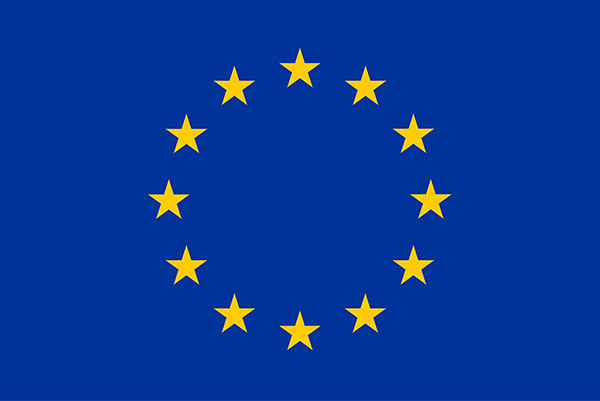
\includegraphics[width=0.15\textwidth]{plots/flag_yellow_low.jpg}
%\end{wrapfigure}
%
No. 2015/19/P/ST2/03007. 
%
The project has received funding from the
European Union's Horizon 2020 research  and  innovation  programme  under  the
Marie Sk\l{}odowska-Curie grant agreement No. 665778.
%
The work of M.C. was supported in part by a grant of the BMBF.
%
R.A.M and S.S acknowledge hospitality of the
Institute for Theoretical Particle Physics and Cosmology, RWTH Aachen
University, where substantial part of this work has been done.
%
We are also grateful to Andreas van Hameren for illuminating discussions
throughout the course of this work.
%
We thank Thomas Hahn for assistance with the Cuba library.
%
This research was supported in part by PLGrid infrastructure.
%
We are grateful for computing resources of ACC Cyfronet AGH where our numerical
calculations were performed on the Prometheus cluster.
%
S.S. would like to acknowledge the Mainz Institute for Theoretical Physics
(MITP) for hospitality and support during the completion of this work.

%-----------------------------------------------------------------------------
\appendix

%-----------------------------------------------------------------------------

%-----------------------------------------------------------------------------
% NOTE:
%
% The colour matrices are derived in 
% ttbar/secdec/double-emission-tensor/input-list.nb
%
%-----------------------------------------------------------------------------
\section{Colour matrices}
\label{app:colmat}

In this appendix, we collect all colour matrices that appear in the formulae
for the soft function at NLO and NNLO, in the basis defined in 
Eqs.~(\ref{eq:colour-basis-qq}) and~(\ref{eq:colour-basis-gg}).

Let us start by determining the set of independent dot products of the operators
$\cT_i$. For the top pair production in the $\iibar$ channel, we have
%
\begin{eqnarray}
  \begin{array}{ll}
    \cT_i^2 =  C_i \unitop\,,  &
    \qquad \text{for the incoming partons } \iibar\,,
    \\
    \cT_i^2 =  C_F \unitop\,, &
    \qquad \text{for the outgoing } \ttbar \text{ pair}\,.
    \label{eq:Ti2}
  \end{array}
\end{eqnarray}
%
The colour conservation 
%
\begin{equation}
  \sum_{i=1}^4 \cT_i |\calM\rangle = 0\,,
  \label{eq:colconsdef}
\end{equation}
%
allows us to write the following set of equations
%
\begin{equation}
 \{\cT_i \cdot \cT_j  = 
 \sum_{\substack{k \neq i \\ m \neq j}} \cT_k \cdot \cT_m \}\,,
  \label{eq:colconservTT}
\end{equation}
%
for $i,j \in \{1,\ldots, 4\}$.
%
By combining~(\ref{eq:Ti2}) and (\ref{eq:colconservTT}), we arrive at the
relations
%
\begin{subequations}
  \label{eq:TiTjrelations}
  \begin{align}
    \cT_1 \cdot \cT_4  & = \cT_2 \cdot \cT_3\,,\\ 
    %
    \cT_2 \cdot \cT_4  & = \cT_1 \cdot \cT_3\,,\\ 
    %
    \cT_1 \cdot \cT_1  & = \cT_2 \cdot \cT_2  =
    -\cT_1 \cdot \cT_3  - \cT_2 \cdot \cT_3  - \cT_1 \cdot \cT_2  \,,\\ 
    %
    \cT_3 \cdot \cT_3  & = \cT_4 \cdot \cT_4  =
    -\cT_1 \cdot \cT_3  - \cT_2 \cdot \cT_3  - \cT_3 \cdot \cT_4  \,.
  \end{align}
\end{subequations}
%
Hence, in general, we have four independent structures: 
$\cT_1 \cdot \cT_3$, $\cT_2 \cdot \cT_3$, $\cT_1 \cdot \cT_2$, $\cT_3 \cdot
\cT_4$. For the \qqbar channel, this number is further reduced to
three, as all $\cT_i\cdot \cT_i$ are equal, which leads to the relation
$\cT_1 \cdot \cT_2 = \cT_3 \cdot \cT_4$.

In the case of the \qqbar channel, the three independent matrices
$\bfw_{ij}^{(1)}$, defined in Eq.~(\ref{eq:w1def}), read
%
\begin{subequations}
  \allowdisplaybreaks
  \begin{align}
  %%%
  \bfw_{13}^{(1)} & = 
  - \frac{C_F}{2}
  \left( \begin{array}{cc}
    0 & 1 \\
    1 & 2 C_F -\frac{N}{2}
  \end{array} \right)\,,
  \\[0.5em]
  %%%
  \bfw_{23}^{(1)} & = 
  - \frac{C_F}{2N}
  \left( \begin{array}{cc}
    0 & -N \\
    -N & 1 
  \end{array} \right)\,,
  \\[0.5em]
  %%%
  \bfw_{34}^{(1)} & = 
  - \frac{C_F}{4N}
  \left( \begin{array}{cc}
    4N^2 & 0 \\
    0 & -1 
  \end{array} \right)\,,
  \end{align}
\end{subequations}
%
while, for the $gg$ channel, we have the following four independent
$\bfw_{ij}^{(1)}$ matrices
%
\begin{subequations}
  \allowdisplaybreaks
  \begin{align}
   %%%
   \bfw_{13}^{(1)} & = 
   -\frac{1}{8}
   \left( \begin{array}{ccc}
     0  & 4N     & 0 \\
     4N & N^2    & N^2-4 \\
     0  & N^2-4  & N^2-4
   \end{array} \right)\,,
   \\[0.5em]
   %%%
   \bfw_{23}^{(1)} & = 
   -\frac{1}{8}
   \left( \begin{array}{ccc}
     0   & -4N     & 0 \\
     -4N & N^2     & -N^2+4 \\
     0   & -N^2+4  & N^2-4
   \end{array} \right)\,,
   \\[0.5em]
   %%%
   \bfw_{12}^{(1)} & = 
   - \frac{1}{4}
   \left( \begin{array}{ccc}
     4N^2 & 0   & 0 \\
     0    & N^2 & 0 \\
     0    & 0   & N^2-1
   \end{array} \right)\,,
   \\[0.5em]
   %%%
   \bfw_{34}^{(1)} & = 
   - 
   \left( \begin{array}{ccc}
     C_F N & 0            & 0 \\
     0     & -\frac{1}{4} & 0 \\
     0     & 0            & -\frac{N^2-4}{4N^2}
   \end{array} \right)\,.
  \end{align}
\end{subequations}

The $\bfw_{ij}^{(2S)}$ matrices, which enter the abelian part of the double-cut
contributions to the soft function (\ref{eq:2cutmaster}), were defined in
Eq.~(\ref{eq:w2def}). In the case of the $\qqbar$ channel, they take the
following explicit forms
%
\begin{subequations}
\allowdisplaybreaks
\begin{align}
    \bfw_{1333}^{(2S)}  & = 
    \left(
    \begin{array}{cc}
     0 & -\frac{\left(N^2-1\right)^2}{4 N^2} \\
     -\frac{\left(N^2-1\right)^2}{4 N^2} & -\frac{\left(N^2-2\right)
    \left(N^2-1\right)^2}{8 N^3} \\
    \end{array}
    \right)
    \,,\\[0.5em]
    %%%
    \bfw_{1433}^{(2S)}  & = 
\left(
\begin{array}{cc}
 0 & \frac{\left(N^2-1\right)^2}{4 N^2} \\
 \frac{\left(N^2-1\right)^2}{4 N^2} & -\frac{\left(N^2-1\right)^2}{4 N^3} \\
\end{array}
\right)
    \,,\\[0.5em]
    %%%
    \bfw_{1314}^{(2S)}  & = 
\left(
\begin{array}{cc}
 -\frac{N^2-1}{2 N} & \frac{1}{8} \left(-N^2+5-\frac{4}{N^2}\right) \\
 \frac{1}{8} \left(-N^2+5-\frac{4}{N^2}\right) & \frac{N^4-4 N^2+3}{8 N^3} \\
\end{array}
\right)
    \,,\\[0.5em]
    %%%
    \bfw_{3334}^{(2S)}  & = 
\left(
\begin{array}{cc}
 -\frac{\left(N^2-1\right)^2}{2 N} & 0 \\
 0 & \frac{\left(N^2-1\right)^2}{8 N^3} \\
\end{array}
\right)
    \,,\\[0.5em]
    %%%
    \bfw_{1334}^{(2S)}  & = 
\left(
\begin{array}{cc}
 0 & \frac{N^4-3 N^2+2}{8 N^2} \\
 \frac{N^4-3 N^2+2}{8 N^2} & -\frac{N^4-3 N^2+2}{8 N^3} \\
\end{array}
\right)
    \,,\\[0.5em]
    %%%
    \bfw_{1434}^{(2S)}  & = 
\left(
\begin{array}{cc}
 0 & -\frac{N^4-3 N^2+2}{8 N^2} \\
 -\frac{N^4-3 N^2+2}{8 N^2} & -\frac{N^2-1}{4 N^3} \\
\end{array}
\right)
    \,,\\[0.5em]
    %%%
    \bfw_{3434}^{(2S)}  & = 
\left(
\begin{array}{cc}
 \frac{\left(N^2-1\right)^2}{2 N} & 0 \\
 0 & \frac{N^2-1}{8 N^3} \\
\end{array}
\right)
    \,,\\[0.5em]
    %%%
    \bfw_{1414}^{(2S)}  & = 
\left(
\begin{array}{cc}
 \frac{N^2-1}{2 N} & \frac{1}{2} \left(\frac{1}{N^2}-1\right) \\
 \frac{1}{2} \left(\frac{1}{N^2}-1\right) & \frac{N^4+2 N^2-3}{8 N^3} \\
\end{array}
\right)
    \,,\\[0.5em]
    %%%
    \bfw_{1313}^{(2S)}  & = 
\left(
\begin{array}{cc}
 \frac{N^2-1}{2 N} & \frac{N^4-3 N^2+2}{4 N^2} \\
 \frac{N^4-3 N^2+2}{4 N^2} & \frac{N^6-4 N^4+6 N^2-3}{8 N^3} \\
\end{array}
\right)
    \,,\\[0.5em]
    %%%
    \bfw_{3333}^{(2S)}  & = 
\left(
\begin{array}{cc}
 \frac{\left(N^2-1\right)^2}{2 N} & 0 \\
 0 & \frac{\left(N^2-1\right)^3}{8 N^3} \\
\end{array}
\right)
\,.
\end{align}
\end{subequations}
%
In the $gg$ channel, these colour matrices read
%
\begin{subequations}
\allowdisplaybreaks
\begin{align}
    \bfw_{1333}^{(2S)}  & = 
\left(
\begin{array}{ccc}
 0 & \frac{1}{2} \left(1-N^2\right) & 0 \\
 \frac{1}{2} \left(1-N^2\right) & -\frac{1}{8} N \left(N^2-1\right) &
-\frac{N^4-5 N^2+4}{8 N} \\
 0 & -\frac{N^4-5 N^2+4}{8 N} & -\frac{N^4-5 N^2+4}{8 N} \\
\end{array}
\right)
    \,,\\[0.5em]
    %%%
    \bfw_{1433}^{(2S)}  & = 
\left(
\begin{array}{ccc}
 0 & \frac{1}{2} \left(N^2-1\right) & 0 \\
 \frac{1}{2} \left(N^2-1\right) & -\frac{1}{8} N \left(N^2-1\right) &
\frac{N^4-5 N^2+4}{8 N} \\
 0 & \frac{N^4-5 N^2+4}{8 N} & -\frac{N^4-5 N^2+4}{8 N} \\
\end{array}
\right)
    \,,\\[0.5em]
    %%%
    \bfw_{1314}^{(2S)}  & = 
\left(
\begin{array}{ccc}
 -N & 0 & 1-\frac{N^2}{4} \\
 0 & -\frac{N}{4} & 0 \\
 1-\frac{N^2}{4} & 0 & \frac{N}{4}-\frac{1}{N} \\
\end{array}
\right)
    \,,\\[0.5em]
    %%%
    \bfw_{3334}^{(2S)}  & = 
\left(
\begin{array}{ccc}
 -\frac{\left(N^2-1\right)^2}{2 N} & 0 & 0 \\
 0 & \frac{N^2-1}{4 N} & 0 \\
 0 & 0 & \frac{N^4-5 N^2+4}{4 N^3} \\
\end{array}
\right)
    \,,\\[0.5em]
    %%%
    \bfw_{1334}^{(2S)}  & = 
\left(
\begin{array}{ccc}
 0 & \frac{1}{4} \left(N^2-2\right) & 0 \\
 \frac{1}{4} \left(N^2-2\right) & -\frac{N}{8} & -\frac{N^2-4}{8 N} \\
 0 & -\frac{N^2-4}{8 N} & -\frac{N^2-4}{8 N} \\
\end{array}
\right)
    \,,\\[0.5em]
    %%%
    \bfw_{1434}^{(2S)}  & = 
\left(
\begin{array}{ccc}
 0 & \frac{1}{4} \left(2-N^2\right) & 0 \\
 \frac{1}{4} \left(2-N^2\right) & -\frac{N}{8} & \frac{N^2-4}{8 N} \\
 0 & \frac{N^2-4}{8 N} & -\frac{N^2-4}{8 N} \\
\end{array}
\right)
    \,,\\[0.5em]
    %%%
    \bfw_{3434}^{(2S)}  & = 
\left(
\begin{array}{ccc}
 \frac{\left(N^2-1\right)^2}{2 N} & 0 & 0 \\
 0 & \frac{1}{4 N} & 0 \\
 0 & 0 & \frac{N^2-4}{4 N^3} \\
\end{array}
\right)
    \,,\\[0.5em]
    %%%
    \bfw_{1414}^{(2S)}  & = 
\left(
\begin{array}{ccc}
 N & -\frac{N^2}{4} & \frac{1}{4} \left(N^2-4\right) \\
 -\frac{N^2}{4} & \frac{1}{8} N \left(N^2+2\right) & -\frac{1}{8} N
\left(N^2-4\right) \\
 \frac{1}{4} \left(N^2-4\right) & -\frac{1}{8} N \left(N^2-4\right) &
\frac{N^3}{8}-\frac{3 N}{4}+\frac{1}{N} \\
\end{array}
\right)
    \,,\\[0.5em]
    %%%
    \bfw_{1313}^{(2S)}  & = 
\left(
\begin{array}{ccc}
 N & \frac{N^2}{4} & \frac{1}{4} \left(N^2-4\right) \\
 \frac{N^2}{4} & \frac{1}{8} N \left(N^2+2\right) & \frac{1}{8} N
\left(N^2-4\right) \\
 \frac{1}{4} \left(N^2-4\right) & \frac{1}{8} N \left(N^2-4\right) &
\frac{N^3}{8}-\frac{3 N}{4}+\frac{1}{N} \\
\end{array}
\right)
    \,,\\[0.5em]
    %%%
    \bfw_{3333}^{(2S)}  & = 
\left(
\begin{array}{ccc}
 \frac{\left(N^2-1\right)^2}{2 N} & 0 & 0 \\
 0 & \frac{\left(N^2-1\right)^2}{4 N} & 0 \\
 0 & 0 & \frac{\left(N^2-4\right) \left(N^2-1\right)^2}{4 N^3} \\
\end{array}
\right)
    \,.
\end{align}
\end{subequations}
%
All the other $\bfw_{ijkl}^{(2S)}$ matrices can be derived from the above set
by using the relations~(\ref{eq:TiTjrelations}).

As for the antisymmetric configurations, $\bm{w}_{ijk}^{(2A)}$, there is only
one independent matrix per channel, which we choose to be $\bm{w}_{123}^{(2A)}$. In the $\qqbar$ channel it reads
%
\begin{eqnarray}
  \bm{w}_{123}^{(2A)} & =
  \frac{1}{8} \left(
  \begin{array}{cc}
  0     & -(N^2-1) \\
  N^2-1 & 0 \\
  \end{array}
  \right)\,,
  \label{eq:w2Aqq}
\end{eqnarray}
%
and in the $gg$ channel
%
\begin{eqnarray}
  \bm{w}_{123}^{(2A)} & =
  \frac{1}{4} \left(
  \begin{array}{ccc}
  0    & -N^2 & 0 \\
  N^2 & 0   & 0 \\
  0    & 0   & 0
  \end{array}
  \right)\,.
  \label{eq:w2Agg}
\end{eqnarray}
%
All the other antisymmetric matrices can be obtained  as combinations of the
above and $\bfw_{ij}^{(1)}$, using colour conservation (\ref{eq:colconsdef}),
together with the relation
%
\begin{equation}
  f^{abc} T^b_i T^c_i = \frac{i}{2} C_A T^a_i\,.
\end{equation}


%-----------------------------------------------------------------------------
\section{Cusp angles}

The amplitudes are functions of Lorentz invariants~\cite{Becher:2009kw}
%
\begin{equation}
  s_{ij} \equiv 2 \sigma_{ij} p_i \cdot p_j + \iep\,,
  \label{eq:sij-def}
\end{equation}
%
and
\begin{equation}
  p_i^2 = m_i^2\,,
  %\label{eq:}
\end{equation}
%
where
%
\begin{eqnarray}
  \sigma_{ij} = \left\{
    \begin{array}{cl} 
      + 1 &  \text{if } p_i, p_j \text{ are both incoming or outgoing} \\
      - 1 &  \text{otherwise}
    \end{array}
    \right.\,.
  %\label{eq:}
\end{eqnarray}
%
For massive particles we define velocities
%
\begin{equation}
  v_i \equiv  \frac{p_i}{m_i}\,,
  \qquad \qquad v_i^2 = 1\,.
  %\label{eq:}
\end{equation}
%
To this end,
we label massless particles with lowercase $i, j, \ldots$ and massive
ones with capital indices $I, J, \ldots$.

The soft anomalous dimension of Eq.~(\ref{eq:softAD}) is a function of
\emph{cusp angles}, $\beta_{ij}$, $\beta_{Ij}$ and $\beta_{IJ}$, formed by
massless and/or massive Wilson lines. They read~\cite{Becher:2009kw}
%
\begin{subequations}
  %\label{eq:}
  \begin{align}
    \beta_{ij} & = 
    \ln \frac{-2 \sigma_{ij}\, p_i \cdot p_j\, \mu^2}{(-p_i^2)(-p_j^2)} =
    L_i + L_j - \ln\frac{\mu^2}{-s_{ij}}\,,
    \\
    \beta_{Ij} & = 
    \ln \frac{-2 \sigma_{ij}\, v_I \cdot p_j\, \mu}{(-p_j^2)} =
    L_j - \ln\frac{m_I \mu}{-s_{ij}}\,,
    \\
   \label{eq:betaIJ-def}
    \beta_{IJ} & =  {\rm arccosh} \left(w_{IJ}\right) = 
                    {\rm arccosh} \left(\frac{-s_{IJ}}{2 m_I m_J}\right)\,,
  \end{align}
\end{subequations}
%
where we have introduced
%
\begin{equation}
  L_i = \ln \frac{\mu^2}{(-p_i^2)}\,,
  %\label{eq:}
\end{equation}
%
which comes from regularization of the IR divergences in the effective theory by
taking massless partons slightly off-shell $(-p_i^2) > 0$~\cite{Becher:2009qa}.
The logarithms $L_i$ need to cancel in the final result for the anomalous
dimension matrix.


%------------------------------------
\subsection*{$\mathbold{\betaIJ}$ in space-like kinematics}

For space-like kinematics of heavy particles (\eg a top quark incoming and a top
quark outgoing), the cusp angle $\beta_{IJ}$ is real. It can still, however, be
chosen to be positive or negative, as the function $\text{arccosh}$ has two
branches, even for real argument. 

The choice of the positive $\betaIJ$ has at least two advantages: (i)
functions that appear in the $\order{\as^2}$ contribution in
Eq.~(\ref{eq:vel-dep-ad}), which we shall discuss in Appendix~\ref{app:AD}, are real (in the space-like case) and do not require
analytic continuation, as $0 < x < 1$ for $\Li_{2,3}(x)$ and for $\ln(x)$, (ii),
$\coth(\betaIJ)$ has a physical interpretation of an inverse of a relative
velocity between particles $I$ and $J$, $\vIJ$, which reads
%
\begin{equation}
  \coth(\betaIJ) = \frac{1}{\vIJ}\,,
  \label{eq:cothbetaIJ}
\end{equation}
%
where
%
\begin{equation}
  v_{IJ} = \sqrt{1- \frac{4 m_t^4}{s_{IJ}^2}}\,.
  %\label{eq:}
\end{equation}
%

The choice $\betaIJ>0$ implies $\vIJ > 0$ and this leads to the following
relation between the latter and the $\beta_t$ function introduced in
Eq.~(\ref{eq:beta-def})
% NOTE
% Derived in my notes \cite{MyNotes}
%
\begin{equation}
  \vIJ = \frac{2 \beta_t}{1+\beta^2_t}\,.
  \label{eq:vIJ-beta-rel}
\end{equation}
%
We notice that
% NOTE
% \cite{MyNotes}
%
\begin{equation}
  \beta_t = \sqrt{\frac{s-1}{s+1}}\,, \qquad \text{where} \qquad 
  s = \frac{\sIJ}{2 m_t^2}\,,
  %\label{eq:}
\end{equation}
%
which means that
%
\begin{equation}
  \begin{array}{lll}
    \text{space-like:}\quad & s < -1 \quad & \beta_t \in [1,\infty)\,, \\[0.5em]
    \text{time-like:}\quad & s > 1 \quad & \beta_t \in [0,1]\,.
  \end{array}
  %\label{eq:}
\end{equation}
%
We also note that $\vIJ \in [0,1]$, both in the space-like and in the time-like
case.


Eq.~(\ref{eq:cothbetaIJ}) has a unique solution for the space-like case with
$\betaIJ >0$ which reads
% NOTE
% \cite{MyNotes}
%
\begin{equation}
  \betaIJ =  -\frac12 \ln \frac{1-\vIJ}{1+\vIJ}\,,
  \label{eq:betaIJ-vIJ}
\end{equation}
%
and, with help of Eq.~(\ref{eq:vIJ-beta-rel}) it can be expressed as
%
\begin{equation}
 \betaIJ = -\frac12 \ln\left[\left(\frac{\beta_t-1}{\beta_t+1}\right)^2\right]
         = \ln\left(\frac{\beta_t+1}{\beta_t-1}\right)\,,
  \qquad \beta_t \in [1,\infty).
  \label{eq:betaIJ-beta}
\end{equation}

%------------------------------------
\subsection*{$\mathbold{\betaIJ}$ in time-like kinematics}
\label{sec:beta34TL}

We would like to analytically continue $\betaIJ$ to the time-like region which
corresponds to $\sIJ > 0$. The function in Eq.~(\ref{eq:betaIJ-beta}) has a cut
at imaginary axis and, depending whether we cross it in the upper or the
lower half-plane, we get a different result.

The convention is already established in Eq.~(\ref{eq:sij-def}).
It implies that the invariant $\sIJ$  has a small
positive part which corresponds to analytic continuation over the upper
half-plane. And this means that $\betaIJ$ acquires an imaginary part $- i \pi$
in the time-like region.
% NOTE
% My notebook ~\cite{AnalyticContinuation}. 
The real part is identical to the one of the space-like kinematics and, at the
end, we get
%
\begin{equation}
  \betaIJ = \ln\left(\frac{1+\beta_t}{1-\beta_t}\right) - i \pi\,,
  \qquad \beta_t \in [0,1]\,.
  \label{eq:beta34TL}
\end{equation}


%-----------------------------------------------------------------------------
\section{Anomalous dimensions and IR renormalization constant}
\label{app:AD}

The cusp anomalous dimension is  given by the following perturbative series
%
\begin{align}
  \label{eq:gammaexp}
  \Gamma_{\text{cusp}}^i(\alpha_s) &= 
  \Gamma_0^i \, \frac{\alpha_s}{4\pi} + 
  \Gamma_1^i \left( \frac{\alpha_s}{4\pi} \right)^2 + 
  \Gamma_2^i \left( \frac{\alpha_s}{4\pi} \right)^3 +
  \ldots \,, 
\end{align}
%
where
%
\begin{equation}
  \Gamma_{n}^i  =  C_i\, \gamma_{n}^\text{cusp}
  \qquad
  \text{ with }
  \qquad
  C_i =  \left\{
  \begin{array}{cc}
    C_F \quad \text{for the $q\bar q$ channel}\,, \\
    C_A \quad \text{for the $gg$ channel}\,,
  \end{array}
  \right.
  %\label{eq:}
\end{equation}
% 
and the coefficients to three loops read
\cite{Moch:2004pa}
%
\begin{align}
  \gamma^{\text{cusp}}_0 &= 4 \, ,
  \nonumber
  \\
  \gamma^{\text{cusp}}_1 &= \left( \frac{268}{9} - \frac{4\pi^2}{3} \right) C_A -
  \frac{80}{9} T_F n_f \, ,
  \nonumber
  \\
  \gamma^{\text{cusp}}_2 &= C_A^2 \left( \frac{490}{3} - \frac{536\pi^2}{27} +
    \frac{44\pi^4}{45} + \frac{88}{3} \zeta_3 \right) + C_A T_F n_f \left( -
    \frac{1672}{27} + \frac{160\pi^2}{27} - \frac{224}{3} \zeta_3 \right) \nonumber
  \\
  &\quad + C_F T_F n_f \left( - \frac{220}{3} + 64 \zeta_3 \right) - \frac{64}{27} T_F^2
  n_f^2 \, .
\end{align}
%
The QCD $\beta$ function is given by
%
\begin{align}
  \label{eq:betaexp}
  \beta(\alpha_s) &= -2\alpha_s \left[ \beta_0 \, \frac{\alpha_s}{4\pi} 
  + \ldots \right] ,
\end{align}
%
where the leading coefficient for $n_f$ flavours of the active, massless quarks,
is
%
\begin{equation}
  \beta_0 = \frac{11}{3} C_A - \frac{4}{3} T_F n_f \,.
  \label{eq:beta0def}
\end{equation}

The soft renormalization factor $\bfZ_s$ can be obtained from the hard
renormalization factor $\bfZ$, determined in Ref.~\cite{Becher:2009cu}, by
discarding all terms proportional to derivatives of the anomalous dimension and
by making the replacement $\bfGamma_n \to \bfgamma^s_n$. 
%
Up to the order $\alpha_s^2$, it reads 
%

\begin{align}
  \bfZ_s & = 1 + \frac{\as}{4\pi} 
  \frac{\bm{\bfgamma^s}_0}{2\epsilon}
  + \left( \frac{\as}{4\pi} \right)^2 \left[
  \frac{\bm{\bfgamma^s}_0}{8\epsilon^2} 
  \left( \bm{\bfgamma^s}_0 -2\beta_0 \right) 
  + \frac{\bm{\bfgamma^s}_1}{4\epsilon} \right] + \mathcal{O}(\alpha_s^3) \,.
\end{align}
%
The soft anomalous dimension
%
\begin{equation}
  \bfgamma^s  = \sum_{n=0}^\infty 
  \left(\frac{\as}{4\pi}\right)^{n+1}\bfgamma^s_n\,,
  %\label{eq:}
\end{equation}
%
has been introduced in
Section~\ref{sec:renormalization}, and its explicit result for processes
involving massive particles reads~\cite{Ahrens:2010zv}
%
\begin{align}
  \bfgamma^s_{q\bar{q}} &= 
  \left[ 
  C_F \,
  \gamma_{\text{cusp}}(\beta_{34},\alpha_s) + 
  2\gamma^Q(\alpha_s) \right] \unitop \nonumber
  \\
  &\quad\mbox{} + \frac{N}{2} \left[ \gamma_{\text{cusp}}(\alpha_s) \, \left(
      \ln\frac{t_1^2}{M^2m_t^2} + i\pi \right) - \gamma_{\text{cusp}}(\beta_{34},\alpha_s)
  \right]
  \begin{pmatrix}
    0 & 0
    \\
    0 & 1
  \end{pmatrix}
  \nonumber
  \\
  &\quad\mbox{} + \gamma_{\text{cusp}}(\alpha_s) \, \ln\frac{t_1^2}{u_1^2} \left[
    \begin{pmatrix}
      0 & \frac{C_F}{2N}
      \\
      1 & -\frac{1}{N}
    \end{pmatrix}
    + \frac{\alpha_s}{4\pi} \, g(\beta_{34})
    \begin{pmatrix}
      0 & \frac{C_F}{2}
      \\
      -N & 0
    \end{pmatrix}
  \right] , 
\end{align}
%
and 
%
\begin{align}
  \bfgamma^s_{gg} &= \left[
  C_F \,
  \gamma_{\text{cusp}}(\beta_{34},\alpha_s) +
  2\gamma^Q(\alpha_s)
  \right] \unitop \nonumber
  \\
  &\quad\mbox{} + \frac{N}{2} \left[ \gamma_{\text{cusp}}(\alpha_s) \, \left(
  \ln\frac{t_1^2}{M^2m_t^2} + i\pi\right) -
  \gamma_{\text{cusp}}(\beta_{34},\alpha_s) \right]
  \begin{pmatrix}
    0 & 0 & 0
    \\
    0 & 1 & 0
    \\
    0 & 0 & 1
  \end{pmatrix}
  \nonumber
  \\
  &\quad\mbox{} + \gamma_{\text{cusp}}(\alpha_s) \, \ln\frac{t_1^2}{u_1^2}
  \left[ \begin{pmatrix}
  0 & \frac{1}{2} & 0
  \\
  1 & -\frac{N}{4} & \frac{N^2-4}{4N}
  \\
  0 & \frac{N}{4} & -\frac{N}{4}
  \end{pmatrix} 
  + \frac{\alpha_s}{4\pi}\,g(\beta_{34})
  \begin{pmatrix}
  0 & \frac{N}{2} & 0
  \\
  -N & 0 & 0 \\
  0 & 0 & 0
    \end{pmatrix}
  \right]\,.
\end{align}

In order to fully determine the above objects, we need the single-particle
massive anomalous dimensions for heavy quarks~\cite{Becher:2009qa,
Becher:2009kw}
%
\begin{align}
  \gamma^Q_0 &= - 2 C_F \, ,
  \nonumber
  \\
  \gamma^Q_1 &= C_F C_A \left( -\frac{98}{9} + \frac{2\pi^2}{3} - 4 \zeta_3 \right) +
  \frac{40}{9} C_F T_F n_f \, ,
\end{align}
%
as well as the velocity-dependent anomalous dimensions~\cite{Becher:2009kw,
Ferroglia:2009ep, Ferroglia:2009ii, Korchemsky:1987wg, Korchemsky:1991zp,
Kidonakis:2009ev}
%
\begin{align}
  \label{eq:vel-dep-ad}
  \gamma^{\text{cusp}}_0(\beta) &= \gamma^{\text{cusp}}_0 \beta \coth \beta
  \, ,
  \nonumber
  \\
  \gamma^{\text{cusp}}_1(\beta) &= \gamma^{\text{cusp}}_1 \beta \coth \beta
  + 8 C_A \Bigg\{ \frac{\pi^2}{6} + \zeta_3 + \beta^2 \nonumber
  \\
  &\quad + \coth^2\beta \bigg[ \Lithree(e^{-2\beta}) + \beta
  \Litwo(e^{-2\beta}) - \zeta_3 + \frac{\pi^2}{6} \beta + \frac{\beta^3}{3}
  \bigg]
  \nonumber
  \\
  &\quad + \coth\beta \bigg[ \Litwo(e^{-2\beta}) - 2\beta
  \ln(1-e^{-2\beta}) - \frac{\pi^2}{6} (1+\beta) - \beta^2 -
  \frac{\beta^3}{3} \bigg] \Bigg\} \,,
\end{align}
%
and the function
%
\begin{align}
  \label{eq:gfunc}
  g(\beta) &= \coth\beta \bigg[ \beta^2 + 2\beta
  \ln(1-e^{-2\beta}) - \Litwo(e^{-2\beta}) + \frac{\pi^2}{6} \bigg] -
  \beta^2 - \frac{\pi^2}{6} \, .
\end{align}


The velocity-dependent cusp anomalous dimensions
$\gamma^{\text{cusp}}(\beta_{34})$ requires careful treatment. It is
unambiguously defined for space-like kinematics, in which case the function
given in Eq.~(\ref{eq:vel-dep-ad}) is real.  In the time-like kinematics,
however, $\gamma^{\text{cusp}}(\beta_{34})$ has to be analytically continued to
the region $\beta \in [0,1]$, as discussed in Appendix~\ref{sec:beta34TL}.

It turns out that the functions $\coth$, $\ln$ and $\Li_{2,3}$, appearing in
Eqs.~(\ref{eq:vel-dep-ad}) and~(\ref{eq:gfunc}), do not develop discontinuities
when going from the space-like to the time-like case. 
%
% NOTE: logs/notebooks/AnalyticContinuatios.nb
%
Hence, in those functions, we just substitute $\beta_{34} \to \displaystyle
\ln\left(\frac{1+\beta_t}{1-\beta_t}\right)$. And then, wherever $\beta_{34}$
appears in a coefficient, we use Eq.~(\ref{eq:beta34TL}). At the end, we obtain
%
% NOTE
% Results from logs/notebooks/CheckQCDFunctions.nb
%
\allowdisplaybreaks
\begin{align}
  \label{eq:vel-dep-ad-explicit}
  %%%% 0
  \gamma^{\text{cusp}}_0(\beta_t) &= 
  -2\, \frac{1+\beta_t ^2}{\beta_t}
  \left\{\ln \left(\frac{1-\beta}{1+\beta}\right) + i \pi\right\}\,,
  \\
  %%%% 1
  \gamma^{\text{cusp}}_1(\beta_t) &= 
  %% real
  \frac{1}{9 \beta_t ^2}\,
  \Bigg\{30\, C_A\, \pi ^2 \beta_t\,  (1-\beta_t)^2 +
  \ln \left(\frac{1-\beta}{1+\beta}\right) 
  \bigg[72\, C_A\, \beta_t \left(1+ \beta_t ^2\right) 
  \ln \left(\frac{4 \beta_t }{(1+ \beta_t)^2}\right)
  \nonumber \\
  &
  \hspace{30pt}
  +\left(1+\beta_t ^2\right)
  \Big[C_A \big(3\, \pi ^2 (\beta_t  (5 \beta_t -8)+5)-134\, \beta_t \big)+
  40\,  T_F n_f \beta_t \Big]
  \nonumber \\
  &
  \hspace{30pt}
  -6\, C_A (1-\beta_t)^2 \ln \left(\frac{1-\beta}{1+\beta}\right) 
  \Big[6\, \beta_t +\left(1+\beta_t ^2\right)
  \ln \left(\frac{1-\beta}{1+\beta}\right)\Big]\bigg]
  \nonumber \\
  & 
  \hspace{30pt}
  +18 C_A \Bigg(\left(1+\beta_t ^2\right)^2 
  \text{Li}_3\left[\left(\frac{1-\beta_t}{1+\beta_t}\right)^2\right]
  -\left(1-\beta_t ^2\right)^2 \zeta (3)
  \nonumber \\
  &
  \hspace{30pt}
  -\left(1+\beta_t ^2\right) 
  \Big[\left(1+\beta_t ^2\right) \ln
  \left(\frac{1-\beta}{1+\beta}\right)- 2, \beta_t \Big]
  \text{Li}_2\left[\left(\frac{1-\beta_t}{1+\beta_t}\right)^2\right]
  \Bigg)
  \Bigg\}
  \nonumber \\
  &
  %% imaginary
  + \frac{i \pi}{9 \beta_t ^2}
  \Bigg\{72\, C_A\, \beta_t  \left(1+\beta_t ^2\right) 
  \ln \left(\frac{4 \beta_t }{(1+\beta_t)^2}\right)
  -18\, C_A\, \left(1+\beta_t ^2\right)^2
  \text{Li}_2\left[\left(\frac{1-\beta_t}{1+\beta_t}\right)^2\right]
  \nonumber \\
  &
  \hspace{30pt}
  -18\, C_A\, (1-\beta_t)^2\ln 
  \left(\frac{1-\beta}{1+\beta}\right) \left[4 \beta_t
  +\left(1+\beta_t ^2\right) \ln
  \left(\frac{1-\beta}{1+\beta}\right)\right]
  \nonumber \\
  &
  \hspace{30pt}
  + \left(1+ \beta_t ^2\right) \Big[C_A  \left(3\,\pi ^2 
  \left(1+ \beta_t ^2\right)-134\, \beta_t \right) +40\,  T_F n_f\, \beta_t\Big]
  \Bigg\}
  \,,
\end{align}
%
and
%
\begin{align}
  g(\beta_t) &=
  -\frac{1}{\beta_t}
  \Bigg\{\left(1+\beta_t ^2\right) 
  \ln \left(\frac{4 \beta_t }{(1+\beta_t)^2}\right) 
  \ln \left(\frac{1-\beta_t }{1+\beta_t}\right)+
  (1-\beta_t)^2 \left(\frac{5 \pi ^2}{12}- 
  \ln\left(\frac{1-\beta_t }{1+\beta_t}
  \right)\right)
  \nonumber \\
  & +\frac12 \left(1+\beta_t ^2\right)
  \Li_2\left[\left(\frac{1-\beta_t}{1+\beta_t}\right)^2\right]
  \Bigg\}
  + \frac{i\pi}{\beta_t} 
  \left\{(1-\beta_t)^2 \ln \left(\frac{1-\beta_t }{1+\beta_t}\right)
  -\left(1+\beta_t ^2\right) \ln
  \left(\frac{4 \beta_t }{(1+\beta_t)^2}\right)\right\}\,.
\end{align}

The functions given explicitly in this Appendix, together with the result for
the NLO soft function, Eq.~(\ref{eq:NLOSFres}), allow for the complete
determination of all the poles and all $L_\perp$-dependent terms of the NNLO
soft function, following the discussion in Section~\ref{sec:renormalization}.

%-----------------------------------------------------------------------------
\bibliographystyle{unsrt}
%\bibliography{precision-qcd}
\documentclass[a4paper,11pt]{report}
\usepackage[a4paper,left=0.99in, right=0.99in,top=1.2in, bottom=1.2in]{geometry}

\usepackage{common-defs}
%\usepackage{cite}
\usepackage{graphicx}
\usepackage{bm,braket}
\usepackage{hyperref}

\numberwithin{equation}{section}

\newcommand{\question}[1]{{\bf Question:} #1}
\newcommand{\slashnbar}{\slashed{\bar n}}
\newcommand{\mixed}{{M}}
\newcommand{\mycite}[1]{{\footnote{\tt  #1}}}
\newcommand{\Litwo}{{\text{Li}_2}}
\newcommand{\Lithree}{{\text{Li}_3}}
\newcommand{\bfS}{\bm{S}}
\newcommand{\tbfS}{{\tilde \bfS}}
\newcommand{\bfH}{\bm{H}}
\newcommand{\bfw}{\bm{w}}
\newcommand{\bfZ}{\bm{Z}}
\newcommand{\bfgamma}{\bm{\gamma}}
\newcommand{\bfGamma}{\bm{\Gamma}}
\newcommand{\bfI}{\bm{1}}
\newcommand{\idop}{{1\hspace{-4pt} 1}}
\newcommand{\wii}[1]{{\bfw_{i\bar i}^{#1}}}
\newcommand{\kp}{k_+}
\newcommand{\km}{k_-}
\newcommand{\lp}{l_+}
\newcommand{\smallcomment}[1]{{\small \it (#1)}}
\newcommand{\Lp}{L_\perp}
\newcommand{\betaIJ}{\beta_{IJ}}
\newcommand{\vIJ}{v_{IJ}}
\newcommand{\sIJ}{s_{IJ}}


\allowdisplaybreaks

\title{\sc Soft Function Notes}
\author{
  Sebastian Sapeta \\ \\
  {\it Institute of Nuclear Physics, Polish Academy of Sciences}, \\ 
  {\it ul. Radzikowskiego 152, 31-342 Krak\'ow, Poland}
}

%-----------------------------------------------------------------------------
\begin{document}
\maketitle

\tableofcontents

%-----------------------------------------------------------------------------
\chapter{Introduction}

The NLO soft function for \ttbar is computed within standard QCD resummation in
\cite{Catani:2014qha} and within SCET in \cite{Ahrens:2010zv, Li:2013mia}. 
%
The last two references differ in that~\cite{Ahrens:2010zv} performs threshold
resummation, while~\cite{Li:2013mia} performs transverse momentum resummation.
The two procedures share some similarities, in particular, treatment of the
hard function is exactly the same, while the treatment of the soft and the
collinear functions are completely different~\cite{Li:2013mia}.

Ref.~\cite{Ferroglia:2012uy} discusses the soft function at NNLO in the limit of
massless top quarks.

%-----------------------------------------------------------------------------
\chapter{Kinematics and notation}

We consider the process
%
\begin{equation}
  N_1(P_1) + N_2(P_2) \to t(p_3) + \bar t(p_4) + X(p_X)\,,
\end{equation}
%
with the LO subprocesses
%
\begin{eqnarray}
  q(p_1) + \bar q(p_2) & \to & t(p_3) + \bar t(p_4)\,, \\
  g(p_1) + g(p_2)      & \to & t(p_3) + \bar t(p_4)\,,
\end{eqnarray}
%
where $p_1 = \xi_1 P_1$ and $p_2 = \xi_2 P_2$.

We define the following variables
%
\begin{equation}
  \begin{array}{ccc}
  s = (P_1 + P_2)^2\,,   &\hspace{30pt} & \hat s = (p_1 + p_2)^2\,, \\[0.5em]
  M^2 = (p_3 + p_4)^2\,, &\hspace{30pt} & t_1 = (p_1-p_3)^2 - m_t^2\,, \\[0.5em]
  u_1 = (p_1-p_4) - m_t^2\,,&\hspace{30pt} & 
  \tau = \displaystyle \frac{M^2+q_T^2}{s}\,, \\[0.5em]
  z = \displaystyle \frac{M^2}{\shat}\,, & & 
  \label{eq:kin-var}
\end{array}
\end{equation}
%
where $q_T$ is the transverse momentum of the \ttbar pair and $m_t$ is the top
mass.

We will also work in coordinate space where the position of the \ttbar pair is
given by 
%
\begin{equation}
  x^\mu = (x_0, x_\perp, x_3)\,,
  %\label{eq:}
\end{equation}
%
where $x_\perp$ is a 2- or $d-2$-dimensional vector in the transverse plane,
depending on whether we work in 4 or in $d$ dimensions. It is convenient to
express its norm through a logarithm
%
\begin{equation}
  L_\perp = \ln\frac{x_T^2\mu^2}{4\, e^{-2\gamma_E}}\,,
  %\label{eq:}
\end{equation}
%
which corresponds to the relation
%
\begin{equation}
  %x_T = \frac{2}{\mu} e^{-\gamma_E+\frac12 L_\perp}\,.
  x_T = \frac{2}{\mu} e^{-\gamma_E+\frac{L_\perp}{2}}\,.
  %\label{eq:}
\end{equation}

%-----------------------------------------------------------------------------
\section{Small transverse momentum vs threshold limit}

Ref.~\cite{Li:2013mia} studies the small transverse momentum limit
%
\begin{equation}
  \shat, M^2, |t_1|, |u_1|, m_t^2 \gg q_T^2 \gg \Lambda^2_\qcd\,,
\end{equation}
%
where only soft or collinear emissions contribute. The small parameter of SCET
expansion is $\lambda = q_T/M$.
 
In Ref.~\cite{Ahrens:2010zv}, threshold limit is discussed, defined as
%
\begin{equation}
  \shat, M^2, |t_1|, |u_1|, m_t^2 \gg \shat (1-z)^2 \gg \Lambda^2_\qcd\,.
\end{equation}
%
Hence, this the limit, where $z\to 1$ and the \ttbar pair is produced almost at
rest. The small parameter of SCET expansion in this case is taken as $\lambda =
(1-z)$.


%-----------------------------------------------------------------------------
\section{Parametrizations of 4-vectors}

It is convenient to introduce the following vectors
%
\begin{equation}
  n = (1,0,0,1)\,,\quad \nbar = (1,0,0,-1)\,, \qquad n\cdot \nbar = 2\,,
  \qquad n^2 = \nbar^2 = 0\,,
  \label{eq:nnbar-defs}
\end{equation}
%
which are the directions of the colliding partons, and
%
\begin{eqnarray}
  k^\mu 
  & =  &
  n\cdot k \frac{\nbar^\mu}{2} + \nbar \cdot k \frac{n^\mu}{2} + 
  k_\perp^\mu \\
  & \equiv & 
  k^+ \frac{\nbar^\mu}{2} +  k^- \frac{n^\mu}{2} + k_\perp^\mu\,.
\end{eqnarray}
%
Notice that $k_\perp$ is a 4-vectors, although with pure transverse part.

The top quark momenta can be written as
%
\begin{equation}
  p_i^\mu = m_t v_i^\mu + k_i^\mu\,,\quad v_i^2 = 1\,,\qquad i=3,4\,,
  \label{eq:hq-momenta}
\end{equation}
%
where $k_i^\mu$ is a residual momentum which scales like the soft mode $k \sim
\Lambda_\text{soft}$.
%
The total 4-momentum of the \ttbar pair is
%
\begin{equation}
  q = p_3 + p_4\,.
\end{equation}

Some more useful notation~\footnote{In our notation $\beta$ is exactly
$\beta_t$ from \cite{Li:2013mia}.}
%
\begin{eqnarray}
  \label{eq:beta-def}
  \beta & = & \sqrt{1-\frac{4 m_t^2}{M^2}}\,,\\[0.7em]
  \xi_1 = \sqrt{\tau} e^y\,, & & \xi_2 = \sqrt{\tau} e^{-y}\,,\\[0.8em]
  x_s & = &\frac{1-\beta}{1+\beta}\,.
  \label{eq:xs-def}
\end{eqnarray}
%
The variable $\beta$ defined above is related to the relative velocity of the
top and anti-top (or, equivalently, velocity of the top quark in the \ttbar rest
frame)~\cite{Ferroglia:2009ii} 
%
\begin{equation}
  |\vec v_t - \vec v_{\bar t}| = 2 \beta\,.
  %\label{eq:}
\end{equation}

We shall use the following parametrizations of the $d$-vectors~\footnote{ 
\question{It seems that parametrization of $v_3$ and $v_4$ is a choice, which
then has consequences on $k_i$s of Eq.~(\ref{eq:hq-momenta}). The choice adopted
here is such that $v_3$ and $v_4$ are back-to-back in 3-dim (so both the
transverse and the longitudinal part) and $\phi_3 = 0$. Hence, the $q_\perp$ of
the pair comes from $k_is$.
}
\label{fnt:param}
}
%
\begin{eqnarray}
  \label{eq:k4v-par-massless}
  k & = & k_0 (1,\ldots,\sin\theta_1\sin\theta_2,
               \sin\theta_1\cos\theta_2,\cos\theta_1)\,, \\
  v_3 & = & \frac{1}{\sqrt{1-\beta^2}}
            (1,\ldots,0,\beta\sin\theta,\beta\cos\theta)\,, \\
  v_4 & = & \frac{1}{\sqrt{1-\beta^2}}
            (1,\ldots,0,-\beta\sin\theta,-\beta\cos\theta)\,.
\end{eqnarray}

The relevant scalar products are
%
\begin{eqnarray}
  v_3 \cdot v_4  & = & \displaystyle \frac{1+\beta^2}{1-\beta^2}\,, \\
  n\cdot v_3 = \nbar \cdot v_4 & = & 
  \frac{1-\beta \cos\theta}{\sqrt{1-\beta^2}}\,, \\
  \nbar\cdot v_3 = n \cdot v_4 & = & 
  \frac{1+\beta \cos\theta}{\sqrt{1-\beta^2}}\,, \\
  n \cdot k & = & k_0 (1-\cos\theta_1)\,, \\
  \nbar \cdot k & = & k_0 (1+\cos\theta_1)\,, \\
  v_3 \cdot k & = & \frac{k_0}{\sqrt{1-\beta^2}}
  (1-\beta\sin\theta_1\cos\theta_2\sin\theta -
  \beta\cos\theta_1\cos\theta)\,, \\
  v_4 \cdot k & = & \frac{k_0}{\sqrt{1-\beta^2}}
  (1+\beta\sin\theta_1\cos\theta_2\sin\theta +
  \beta\cos\theta_1\cos\theta)\,.
\end{eqnarray}

And, in particular
%
\begin{align}
 k_0 & = \frac12\left(n\cdot k + \nbar \cdot k\right) 
       = \frac12\left(k_+ + k_-\right)\,.
 k_0 & = \frac12\left(n\cdot k + \nbar \cdot k\right) 
       = \frac12\left(k_+ + k_-\right)\,.
\end{align}

We shall also use the $v_{3,4}$ vectors with slightly different normalization
%
\begin{equation}
  \tilde v_3 = \sqrt{1-\beta^2}\, v_3\,,
  \qquad \qquad
  \tilde v_4 = \sqrt{1-\beta^2}\, v_4\,,
  \label{eq:v3v4-tilde-def}
\end{equation}
%
hence
%
\begin{eqnarray}
  \tilde v_3 & = & (1,\ldots,0,\beta\sin\theta,\beta\cos\theta)\,, \\
  \tilde v_4 & = & (1,\ldots,0,-\beta\sin\theta,-\beta\cos\theta)\,.
\end{eqnarray}
%
And the scalar products involving those vectors read
%
\begin{eqnarray}
  \tilde v_3 \tilde v_3  =  \tilde v_4 \tilde v_4 & = & 1-\beta^2
  \\
  \tilde v_3 \cdot \tilde v_4  & = & 1+\beta^2\,, \\
  n\cdot \tilde v_3 = \nbar \cdot \tilde v_4 & = & 1-\beta \cos\theta\,, \\
  \nbar\cdot \tilde v_3 = n \cdot \tilde v_4 & = & 1+\beta \cos\theta\,, \\
  \tilde v_3 \cdot k & = & k_0 (1-\beta\sin\theta_1\cos\theta_2\sin\theta -
  \beta\cos\theta_1\cos\theta)\,, \\
  \tilde v_4 \cdot k & = & k_0 (1+\beta\sin\theta_1\cos\theta_2\sin\theta +
  \beta\cos\theta_1\cos\theta)\,.
\end{eqnarray}

The angles have the following meaning:
 
\begin{center}
  \begin{tabular}{cl}
    $\theta\ $ & scattering angle of the top quark in the \ttbar rest frame \\
    $\phi_t\ $ & azimuthal angle of $v_3$ \\
    $\phi_q\ $ & azimuthal angle of $q_\perp$ \\
    $\phi_x\ $ & azimuthal angle of $x_\perp$  \\
    $\phi\   $ & relative azimuthal angle between $x_\perp$ and $v_3$
  \end{tabular}
\end{center}

%-----------------------------------------------------------------------------
\newpage
\section{Rapidity}

\begin{figure}[t]
  \begin{center}   % width, height
    \begin{picture}(200,140)
    \thicklines
    \put(200,60){\vector(-3,0){80}} 
    \put(0,60){\vector(3,0){80}} 
    \thicklines
    \put(85,70){\vector(-3,2){70}} 
    \put(115,50){\vector(3,-2){70}} 
    \put(90,120){\makebox[30pt]{$(m_{T3}\cosh y_3, p_{T3}, m_{T3}\sinh y_3)$}}
    \put(80,0  ){\makebox[30pt]{$(m_{T4}\cosh y_4, p_{T4}, m_{T4}\sinh y_4)$}}
    \put(0,70 ){\makebox[30pt]{
    $(\frac{\sqrt{s}}{2} \xi_1,0, \frac{\sqrt{s}}{2} \xi_1)$}}
    \put(160,70 ){\makebox[30pt]{
    $(\frac{\sqrt{s}}{2} \xi_2,0, -\frac{\sqrt{s}}{2} \xi_2)$}}
    \end{picture}
  \end{center}
  \caption{Small-$q_T$ kinematics. Four-vectors denoted as $(E,p_T,p_z)$.
  }
  \label{fig:smallqT-kin}
\end{figure}

Assuming that $q_T$ is negligible, we can treat our process as $ij \to \ttbar$
scattering, with the four-momenta as denoted in Fig.~\ref{fig:smallqT-kin}.
%
Small-$q_T$ approximation implies $p_{T3} \simeq p_{T4}$, hence
$m_{T3} \simeq m_{T4} \equiv m_{Tt}$. By comparing the energies and longitudinal
momenta of the incoming and the outgoing particles, we get
%
\begin{subequations}
  \label{eq:222kin}
  \begin{align}
  \xi_1 & =  \frac{m_{Tt}}{\sqrt{s}} \left(e^{y_3} + e^{y_4}\right)\,,
  \\
  \xi_2 & =  \frac{m_{Tt}}{\sqrt{s}} \left(e^{-y_3} + e^{-y_4}\right)\,.
  \end{align}
\end{subequations}
%
From general considerations (see \eg \cite{Ellis}), we have
%
\begin{subequations}
  %\label{eq:}
  \begin{align}
  y_3 & = y + \ybar \,, \\
  y_4 & = y - \ybar \,,
  \end{align}
\end{subequations}
%
where $y$ is the rapidity of the $\ttbar$ system and $\ybar$ is the rapidity of
the $t$ quark in the $\ttbar$ rest frame. This allows us to write
Eqs.~(\ref{eq:222kin}) as
%
\begin{subequations}
  %\label{eq:}
  \begin{align}
  \frac{\xi_1 \sqrt{s}}{2 m_{Tt}} & = e^{y} \cosh \ybar\,, \\
  \frac{\xi_2 \sqrt{s}}{2 m_{Tt}} & = e^{-y} \cosh \ybar\,,
  \end{align}
\end{subequations}
%
which leads to the formula for the rapidity of the $\ttbar$ system
%
\begin{equation}
  y = \frac12 \ln\frac{\xi_1}{\xi_2}\,,
  %\label{eq:}
\end{equation}
and the relation between $\xi_1, \xi_2$ and the integration variables used in
Ref.~\cite{Li:2013mia} and in my program, reads
%
\begin{equation}
  %\label{eq:}
  \xi_1 = z_1 x\,, \qquad
  \xi_2  = z_2 \frac{\tau}{xz_1 z_2} = \frac{\tau}{xz_1}\,,
\end{equation}
%
which gives
\begin{equation}
  y = \frac12 \ln \left[\frac{z_1^2 x^2 }{\tau} \right]
    = \ln \left[\frac{z_1 x }{\sqrt{\tau}} \right]\,.
  %\label{eq:}
\end{equation}

%-----------------------------------------------------------------------------
\newpage
\chapter{General considerations}

The general formula for the soft function reads~\cite{Ahrens:2010zv}, 
Eq.~(3.26)~\footnote{
In the threshold region, $z\to 1$, not considered here but extensively discussed
in~\cite{Becher:2007ty}, the soft function simplifies 
$\mathbold{W}(x,\mu) \to \mathbold{W}(x^0, \vec x = 0, \mu)$.
}
%
\begin{equation}
  \mathbold{W} (x,\mu) = \frac{1}{d_R} 
  \langle 0| \mathbold{\bar T} [O_s^\dagger (x)] \mathbold{T} [O_s(0)] 
  |0 \rangle\,,
\end{equation}
%
where $\mathbold{\bar T}$ and $\mathbold{T}$ represent time and anti-time
ordering~\cite{Becher:2007ty}.
%
The $O_s^\dagger$ and $O_s$ operators depend on the process under consideration.

For the \ttbar production in \qqbar channel~\cite{Li:2013mia}
%
\begin{equation}
  O_s(x) = S_{v_3}^\dagger(x) S_{v_4}(x) S_{\nbar}^\dagger(x) S_{n}(x)\,,
\end{equation}
%
and in the $gg$ channel ~\cite{Li:2013mia}
%
\begin{equation}
  O_s(x) = S_{v_3}^\dagger(x) S_{v_4}(x) 
  S_{\nbar}^{\text{adj} \dagger}(x) S_{n}^\text{adj}(x)\,.
\end{equation}

The soft Wilson lines are defined as
%
\begin{subequations}
  \begin{align}
    [S_n(x)]^{ab}  & =  \calP \exp 
    \left( ig \int^0_{-\infty}\!\! dt\, n \cdot A_s^c(x+t\, n)\, t^c_{ab}
    \right)\,, \\
    [S_n^\text{adj}(x)]^{ab}  & =  \calP \exp 
    \left( ig \int^0_{-\infty}\!\! dt\, n \cdot A_s^c(x+t\, n)\, 
    (-i f^{cab})
    \right)\,,
  \end{align}
\end{subequations}

To evaluate diagrams corresponding to the soft function at a given order we use
the following rules~\cite{Ahrens:2010zv}:
%
\begin{itemize}
  \item
  associate the eikonal factor $\displaystyle \frac{v_i^\mu}{k \cdot v_i}$
  multiplied by the colour generator $\mathbold{T}_i$ for each attachment of a
  gluon to a particle with velocity $v_i$ (for the incoming, massless particles
  $v_1 = n$ and $v_2 = \nbar$),
  \item
  contract with the cut gluon propagator in position space, which, in Feynman
  gauge, reads
  %
  \begin{equation}
    D^{\mu\nu}_+ (x) = 
    -g^{\mu\nu} \int \frac{d^d k}{(2\pi)^d}
    e^{-i k \cdot x} (2\pi) \delta(k^2) \theta(k^0)\,.
  \end{equation}
\end{itemize}

%------------------------------------
\section{Soft limit and threshold limit}

In the soft limit~\cite{AntoniaMTh}, using the notation $(+,-,\perp)$, we have
%
\begin{equation}
  \begin{array}{lp{20pt}l}
  \text{\ttbar 4-momentum}                   & & q^\mu \sim (1,1,\lambda) \\
  \text{\ttbar position in coordinate space} & & 
      x^\mu \sim (1,1,\lambda^{-1}) \\
  \text{gluon's 4-momentum}                   & & 
      k^\mu \sim (\lambda,\lambda,\lambda) \\
  \end{array}
\end{equation}
%
(see~\cite{Becher:2010tm} for derivation of $x^\mu$ scaling) which gives
%
\begin{equation}
  k \cdot x \simeq k_\perp \cdot x_\perp\,,
\end{equation}
%
which is of order $\order{1}$ and the neglected terms are of order
$\order{\lambda}$. That implies that the gluon propagators takes the following
form in the soft limit
%
\begin{equation}
  D^{\mu\nu,\, \text{soft}}_{+} (x_\perp) = 
  -g^{\mu\nu} \int \frac{d^d k}{(2\pi)^d}
  e^{-i k_\perp \cdot x_\perp} (2\pi) \delta(k^2) \theta(k^0)\,.
\end{equation}

In the threshold limit~\cite{Ahrens:2010zv}, using the notation $(0,3,\perp)$,
we obtain
%
\begin{equation}
  \begin{array}{lp{20pt}l}
  \text{\ttbar 4-momentum}                   & & q^\mu \sim (\lambda,1,1) \\
  \text{\ttbar position in coordinate space} & & 
      x^\mu \sim (\lambda^{-1},1,1) \\
  \text{gluon's 4-momentum}                   & & 
      k^\mu \sim (\lambda,\lambda,\lambda) \\
  \end{array}
\end{equation}
%
which gives
%
\begin{equation}
  k \cdot x \simeq k_0 \cdot x_0\,,
\end{equation}
%
which is of order $\order{1}$ and the neglected terms are of order
$\order{\lambda}$. That implies that, in the threshold limit, the gluon
propagators takes the form~\cite{Ahrens:2010zv}
%
\begin{equation}
  D^{\mu\nu,\, \text{threshold}}_{+} (x_0) = 
  -g^{\mu\nu} \int \frac{d^d k}{(2\pi)^d}
  e^{-i k_0 \cdot x_0} (2\pi) \delta(k^2) \theta(k^0)\,.
\end{equation}

Comment:
%
The above derivation is tentative. I do not have full understanding of
relevant regions here. In particular~\cite{Li:2013mia} mentions that threshold
limit corresponds to ultra-soft region $k^\mu \sim
(\lambda^2,\lambda^2,\lambda^2)$. Perhaps that is because the \ttbar pair is
produced at rest.
%
The important difference is that in the threshold limit we do not need the
regulator $(\nu/k_+)^\alpha$.
%
It is probably related to the fact mentioned in~\cite{Becher:2011dz} that the
ultra-soft emissions do not contribute to the $q_T$ spectrum. So the ultra-soft
limit would be stronger than soft limit relevant for $q_T$ spectra.

%------------------------------------
\section{Analytic regulator}

The following regulator is introduced in phase space
integrals~\cite{Becher:2011dz}
%
\begin{equation}
 \int d\mu(k) = \int d^d k 
 \left(\frac{\nu_+}{k_+}\right)^\alpha \delta(k^2) \theta(k_0).
  %\label{eq:}
\end{equation}
%
This regulator becomes necessary once QCD diagrams are expanded in different
momentum regions relevant for the effective theory. Full QCD does not have these
divergences so after all diagrams are combined, the full result stays finite in
the limit $\alpha \to 0$.
%
In the ultra soft mode $k\sim M \lambda^2  = q_T^2/M$, the above regulator is
not needed. It affects only the modes whose transverse components scale as
$k_\perp \sim q_T$.


%------------------------------------
\section{Perturbative expansion}
\label{eq:soft-func-pert-exp}

The soft function can be expanded perturbatively
%
\begin{equation}
  \mathbold{W} = 
  \mathbold{W}^{(0)} +
  \mathbold{W}^{(1)} \left(\frac{\as}{4\pi} \right) +
  \mathbold{W}^{(2)} \left(\frac{\as}{4\pi} \right)^2 + \ldots
\end{equation}
%
and each order can be decomposed in the colour
space~\cite{Li:2013mia,Ferroglia:2012uy}
%
\begin{eqnarray}
  \mathbold{W}^{(1)}_\text{bare} (\epsilon, x, \mu) & = &
  \sum_{j,k} \mathbold{w}_{jk}\, I_{jk}\,, \\
  \mathbold{W}^{(2)}_\text{bare} (\epsilon, x, \mu) & = &
  \sum_{i} \mathbold{w}_{i}\, I_{i}\,,
\end{eqnarray}
%
where $\mathbold{w}$ are the colour matrices at a given order and $I$ are the
NLO and NNLO the integrals defined in the following sections.


%-----------------------------------------------------------------------------
\section{Colour basis}
\label{sec:colbasis}

Following~\cite{Li:2013mia, Ferroglia:2012uy}, we define the basis
vectors 
$|c_I\rangle = \big(c_I^{ij}\big)_{\{a\}}$ 
of the colour space in the $q\qbar$ channel
%
\begin{eqnarray}
  \left(c_1^{q\bar{q}}\right)_{\{a\}} & = & \delta_{a_1a_2} \,\delta_{a_3a_4}\,,
  \\
  \left(c_2^{q\bar{q}}\right)_{\{a\}} & = & t_{a_1a_2}^c \, t_{a_3a_4}^c\,,
\end{eqnarray}
%
and in the $gg$ channel
%
\begin{subequations}
  \begin{align}
    \left(c_1^{gg}\right)_{\{a\}} & = \delta^{a_1a_2} \, \delta_{a_3a_4} \, , 
    \\
    \left(c_2^{gg}\right)_{\{a\}} & = i f^{a_1a_2c} \, t^{c}_{a_3a_4} \, , 
    \\
    \left(c_3^{gg}\right)_{\{a\}} & = d^{a_1 a_2 c} \, t^c_{a_3a_4} \, .
  \end{align}
  \label{eq:colour-basis-gg}
\end{subequations}
%
The inner product is defined as a sum over all colour indices
%
\begin{equation}
  \langle c_I | c_J \rangle = 
  \sum_{\{a\}} 
  \left( c_I \right)^*_{a_1 a_2 a_3 a_4}
  \left( c_J \right)_{a_1 a_2 a_3 a_4}\,.
  %\label{eq:}
\end{equation}
%
The basis vectors are orthogonal but not orthonormal~\cite{Ferroglia:2012uy}.

%-----------------------------------------------------------------------------
\section{Averaged soft function}

The soft function can be averaged over the azimuthal angle. In 4 dimensions one gets
%
\begin{equation}
  \bfS_{i\bar i} = \int \frac{d\phi}{2\pi} \bm{W}_{i\bar i}\,.
  \label{eq:sf-av4}
\end{equation}
%
It can also be expanded as 
\begin{equation}
  \bfS_{i\bar i} = 
  \sum_{n=0}^\infty \bfS_{i\bar i}^{(n)} \left(\asp\right)^n\,.
  %\label{eq:}
\end{equation}
The above equation holds both for bare and renormalized quantities as long as
the all objects, \ie $\bfS_{\iibar}$, $\bfS_{\iibar}^{(n)}$ and $\as$,  are of
the same type.

It turns out to be convenient to generalize Eq.~(\ref{eq:sf-av4}) to $d$
dimensions where it reads
%
\begin{equation}
  \bfS_{i\bar i} = \int \frac{d\Omega_{d-3}}{S_{d-3}} \bm{W}_{i\bar i}\,,
  \label{eq:sf-avd}
\end{equation}
%
with $d\Omega_{d-3}$ being a rotationally-invariant measure on the unit
$d-3$-sphere with the surface~$S_{d-3}$.

%-----------------------------------------------------------------------------
\section{Transformations between coordinate and momentum space}
\label{sec:trans-coor-mom}

In practice, it is easier to calculate the soft function in momentum space. The
relevant scalar integrals are related through Fourier transform
%
\begin{subequations}
   \label{eq:fourier-transformd}
   \begin{eqnarray}
     \tilde I_{jk} (q_\perp)& = &
     \frac{1}{\left(2\pi\right)^{\frac{d-2}{2}}}
     \int d^{d-2} x_\perp I_{jk} (x_\perp) \, e^{i x_\perp \cdot q_\perp}\,,
     \\
      \label{eq:fourier-transform-inv}
      I_{jk} (x_\perp)& = &
     \frac{1}{\left(2\pi\right)^{\frac{d-2}{2}}}
     \int d^{d-2} q_\perp \tilde I_{jk} (q_\perp) \, e^{-i x_\perp \cdot
     q_\perp}\,.
   \end{eqnarray}
\end{subequations}
%
The structure of the $I_{jk}(x_\perp)$ integrals is
%
\begin{equation}
  I_{jk}(x_\perp) = 
  \int \frac{d^dk}{(2\pi)^{d-1}} f(k)\, e^{-i x_\perp \cdot k_\perp}\,.
  %\label{eq:}
\end{equation}
%
The above structure is general and it applies to any double and single-cut
diagrams. In the former case, $f(k)$ is itself an integral with the measure
$d^dl$ and $k$ is the sum of the cut gluons' momenta.
%
Hence, the Fourier transform gives
%
\begin{align}
  \tilde I_{jk}(q_\perp) 
  & = 
  \frac{1}{\left(2\pi\right)^{\frac{d-2}{2}}}
  \int d^{d-2} x_\perp
  \int \frac{d^dk}{(2\pi)^{d-1}}f(k)\, e^{-i x_\perp \cdot (k_\perp-q_\perp)}
  \nonumber \\
  & = 
  \frac{1}{\left(2\pi\right)^{\frac{d-2}{2}}}
  \int \frac{d^dk}{(2\pi)^{d-1}}f(k)\,
  (2\pi)^{d-2}\, \delta^{(d-2)}(q_\perp-k_\perp)
  \nonumber \\
  & = 
  \frac{1}{\left(2\pi\right)^{\frac{d}{2}}}
  \int d^dk\, f(k)\, \delta^{(d-2)}(q_\perp-k_\perp)
  \nonumber \\
  & = 
  \frac{1}{\left(2\pi\right)^{\frac{d}{2}}}
  \int dk_+ dk_-d^{d-2}k_\perp\, f(k)\, \delta^{(d-2)}(q_\perp-k_\perp)\,.
\end{align}
%
In the averaged case, corresponding to Eq.~(\ref{eq:sf-avd}),
%%
%\begin{equation}
%  f(k) = \int\frac{d\Omega_{d-3}}{S_{d-3}} \tilde f(k)\,,
%  %\label{eq:}
%\end{equation}
%%
we get~\cite{mymath}
%
\begin{align}
  \tilde I_{jk}(q_T) 
  & = 
  \frac{1}{\left(2\pi\right)^{\frac{d}{2}} S_{d-3}}
  \int dk_+ dk_- \frac{dk_T}{k_T^{d-3}}\, f(k)\, \delta(q_T-k_T)
  \nonumber \\
  & = 
  \frac{1}{\left(2\pi\right)^{\frac{d}{2}} S_{d-3}}
  \int dk_+ dk_- dk_T\, \frac{\tilde f(k)\,}{q_T^{d-2+n}} \delta(1-k_T)
  \nonumber \\
  & \equiv
  \frac{1}{\left(2\pi\right)^{\frac{d}{2}} S_{d-3}}
  \int dk_+ dk_- dk_T\, \frac{\tilde f(k)\,}{q_T^{p}} \delta(1-k_T)\,.
\end{align}
%
Above, the overall power of $q_T$ has been denoted as $p$. It is a sum of the
contribution from the $d-2$-dimensional delta function and a genuine
contribution from the matrix element $n$.
%
Hence, we see that our function $\tilde I_{jk}(q_T)$ factorizes as
%
\begin{align}
  \tilde I_{jk}(q_T) 
  & = 
  \frac{1}{q_T^{p}}  \,
  \frac{1}{\left(2\pi\right)^{\frac{d}{2}} S_{d-3}}
  \int dk_+ dk_- dk_T\, \tilde f(k)\delta(1-k_T)\,.
\end{align}

Now, we apply inverse Fourier transform to the $1/q_T^p$  factor
%
\begin{align}
  \text{FT}\left[\frac{1}{q_T^p}\right] 
   & =
  \frac{1}{\left(2\pi\right)^{\frac{d-2}{2}}}
  \int d^{d-2} q_\perp \frac{1}{q_T^p} \, e^{-i x_\perp \cdot q_\perp}
  \nonumber \\
   & =
  \frac{S_{d-4}}{\left(2\pi\right)^{\frac{d-2}{2}}}
  \int d\theta \sin^{d-4}\theta\, dq_T q_T^{d-3-p} e^{-i x_T q_T \cos\theta}\,.
  \nonumber \\
\end{align}
%
The integration can be performed exactly and we obtain
\begin{align}
  \text{FT}\left[\frac{1}{q_T^p}\right] 
   & =
   \sqrt{\pi}
   \left(\frac{2}{\mu}e^{-\gamma_E}\right)^{-2+p}
   e^{-(1-\frac{p}{2})L_\perp}
   \frac{\Gamma(2-p)}{\Gamma\left(\frac{3}{2}-
   \frac{p}{2}\right)\Gamma\left(\frac{p}{2}\right)}.
\end{align}

%-----------------------------------------------------------------------------
\section{Renormalized soft function}

The soft function needs to be renormalized by removing all the poles in
$\epsilon$. The prescription reads
%
\begin{equation}
  \bfS_{i\bar i}^{r\text{(en)}} = 
  \bfZ_{i\bar i}\, \bfS_{i\bar i}^{b\text{(are)}}\,, 
  %\label{eq:}
\end{equation}
%
where the coefficient is determined such that it absorbs all poles order by
order.

Up to the $\order{\as^2}$ one can write
%
\begin{eqnarray}
  \bfS_{i\bar i}^{r (0)} + 
  \asp \bfS_{i\bar i}^{r (1)}  +
  \left(\asp \right)^2 \bfS_{i\bar i}^{r (2)} 
  & = &
  \left[\bfZ_{i\bar i}^{(0)} + \asp \bfZ_{i\bar i}^{(1)} +
  \left(\asp\right)^2 \bfZ_{i\bar i}^{(2)}
  \right]
  %\label{eq:}
  \\
  & &
  %\hspace{-10pt}
  \times \left[
  \bfS_{i\bar i}^{b (0)} + 
  \asp \bfS_{i\bar i}^{b (1)}  +
  \left(\asp \right)^2 \bfS_{i\bar i}^{b (2)} 
  \right]\,,
  \nonumber
\end{eqnarray}
%
which leads to the following relations
%
\begin{eqnarray}
  %%%
  \bfS_{i\bar i}^{r (0)}
  & = &
  \bfZ_{i\bar i}^{(0)} \bfS_{i\bar i}^{b (0)}\,,
  \\
  %%%
  \label{eq:ren-id-1}
  \bfS_{i\bar i}^{r (1)}
  & = &
  \bfZ_{i\bar i}^{(1)} \bfS_{i\bar i}^{b (0)} +
  \bfZ_{i\bar i}^{(0)} \bfS_{i\bar i}^{b (1)}\,,
  \\
  %%%
  \bfS_{i\bar i}^{r (2)}
  & = &
  \bfZ_{i\bar i}^{(2)} \bfS_{i\bar i}^{b (0)} +
  \bfZ_{i\bar i}^{(1)} \bfS_{i\bar i}^{b (1)} +
  \bfZ_{i\bar i}^{(0)} \bfS_{i\bar i}^{b (2)}\,.
\end{eqnarray}

%-----------------------------------------------------------------------------
\chapter{LO and NLO soft function}

%-----------------------------------------------------------------------------
\section{LO soft function}

The leading soft function is computed with
%
\begin{equation}
  \left(\bfS_{i\bar i}^{b (0)}\right)_{IJ} = 
  \frac{1}{N_i} \langle c_I | c_J \rangle\,,
  %\label{eq:}
\end{equation}
%
as it corresponds to the case without soft radiation. The explicit expressions
in the $q\qbar$ and the $gg$ channel read
%
\begin{subequations}
\begin{eqnarray}
 \bfS^{b(0)}_{q\qbar} & =  &
 \left( \begin{array}{cc}
   N & 0 \\
   0 & \frac{C_F}{2} 
 \end{array} \right)\,,
 \\[0.5em]
 \bfS^{b(0)}_{gg} & =  &
 \left( \begin{array}{ccc}
   N & 0           & 0 \\
   0 & \frac{N}{2} & 0 \\
   0 & 0           & \frac{N^2-4}{2N}
 \end{array} \right)\,.
\end{eqnarray}
 \label{eq:Sii-LO}
\end{subequations}
%
Because the leading order soft function is not divergent
\begin{equation}
 \bfS^{r(0)}_{q\qbar}  = \bfS^{b(0)}_{q\qbar}\,,  
 \qquad \qquad \qquad
 \bfS^{r(0)}_{gg}  = \bfS^{b(0)}_{gg}\,,  
  %\label{eq:}
\end{equation}
%
and hence
%
\begin{equation}
  \bfZ_{i\bar i}^{(0)} =  \idop\,.
  \label{eq:Z0-res}
\end{equation}

%-----------------------------------------------------------------------------
\section{NLO soft function}
\label{sec:nlo-soft-function}

The NLO soft functions reads
%
\begin{equation}
  \bfS_{i\bar i}^{b(1)} = 
  \sum_{j,k} \bm{w}_{jk}^{i\bar i} I_{jk}\,,
  \label{eq:S-W-Ijk}
\end{equation}
%
where the colour structure is encoded in in the $\bm{w}_{jk}^{i\bar i}$ matrices
defined in the following way with the basis of Section~\ref{sec:colbasis}
%
\begin{equation}
  \left(\bm{w}_{jk}^{i\bar i}\right)_{IJ} =
  \frac{1}{N_i} \langle c_I |\bm{T}_i \cdot \bm{T}_j | c_J \rangle\,,
  %\label{eq:}
\end{equation}
%
where we collect for completeness in Appendix~\ref{app:wmatrices}.

The starting point for the computation of the NLO soft integrals 
is~\cite{AntoniaMTh}
%
\begin{equation}
  I_{jk} = 
  -(4\pi)^2 
  \left(\frac{\mu^2 e^{\gamma_E}}{4\pi}\right)^\epsilon
  \int_0^{2\pi} \frac{d\phi}{2\pi}
  \int \frac{d^d k}{(2\pi)^{d-1}}
  \left(\frac{\nu}{k_+}\right)^\alpha
  \delta(k^2)\, \theta(k^0)\,
  \frac{v_j \cdot v_k}{v_j \cdot k\; v_k \cdot k}
  e^{-i x_\perp \cdot k_\perp}\,,
\end{equation}
%
which contains the $e^{\epsilon \gamma_E} (4\pi)^{-\epsilon}$ factor coming from
\msbar renormalization but other than that it is still a bare function. (In
other words, one will only need to remove poles, like in MS scheme, to
renormalize it.)
%
The above formula can be simplified~to~\footnote{
This result agrees with \cite{AntoniaMTh}, page 93. Note there is a difference
with respect to Eq.~(38) of \cite{Li:2013mia}, which comes from the fact that
the latter does not include the \msbar factor.}
%
\begin{equation}
  I_{jk} = 
  -\frac{\mu^{2\epsilon} e^{\epsilon \gamma_E}}{\pi^{2-\epsilon}}
  \int_0^{2\pi} d\phi
  \int d^d k
  \left(\frac{\nu}{n\cdot k}\right)^\alpha
  \delta(k^2)\, \theta(k^0)\,
  \frac{v_j \cdot v_k}{v_j \cdot k\; v_k \cdot k}
  e^{-i x_\perp \cdot k_\perp}\,.
  \label{eq:NLOsoft-function-def}
\end{equation}

%-----------------------------------------------------------------------------
\subsection{Soft integrals in momentum space}

Following the discussion in Sec.~\ref{sec:trans-coor-mom}, the
azimuthal-volume-averaged soft function integrals at NLO read
%
\begin{equation}
  \tilde I_{jk} = 
  -\frac{\calN (4\pi)^2}{(2\pi)^{\frac{d}{2}} S_{d-3}}
  \left(\frac{\mu^2 e^{\gamma_E}}{4\pi}\right)^\epsilon 
  \int \frac{d^d k}{k_T^{d-3}}
  \left(\frac{\nu}{n\cdot k}\right)^\alpha
  \delta(k^2)\, \theta(k^0)\,
  \delta(k_T - q_T)
  \frac{v_j \cdot v_k}{v_j \cdot k\; v_k \cdot k}\,,
  \label{eq:soft-func-nlo-mom-space-ddim}
\end{equation}
%
where, $\calN = 2 $ in order for the final result to match that of
Ref.~\cite{Li:2013mia}, a convention I still need to understand. 
%
In the above, the
factor $\left(\frac{\mu^2 e^{\gamma_E}}{4\pi}\right)^\epsilon$ comes from
renormalization of the strong coupling, the minus sign comes from sum over
polarizations leading to $-g^{\mu\nu}$ and $(4\pi)^2$ comes from taking this
factor out in the form of $\frac{\as}{4\pi} = \frac{g^2}{(4\pi)^2}$.

Eq.~(\ref{eq:soft-func-nlo-mom-space-ddim}) already allows one to deduce the
dependence on $q_T$. Indeed by rescaling all components of $k$ by $q_T$ we
obtain
%
\begin{equation}
  \tilde I_{jk} = 
  -\frac{\calN (4\pi)^2 \nu^\alpha}{(2\pi)^{\frac{d}{2}} S_{d-3}}
  \left(\frac{\mu^2 e^{\gamma_E}}{4\pi}\right)^\epsilon 
  \frac{1}{q_T^{2+\alpha}}
  \int \frac{d^d k}{k_+^\alpha\, k_T^{d-3}}
  \delta(k^2)\, \theta(k^0)\,
  \delta(k_T - 1)
  \frac{v_j \cdot v_k}{v_j \cdot k\; v_k \cdot k}\,.
  \label{eq:soft-func-nlo-mom-space-rescal}
\end{equation}

\subsubsection{Results at the boundary}

The integral (\ref{eq:soft-func-nlo-mom-space-rescal}) can be easily calculated
at the boundary, \ie for $\beta=0$. For example
%
\begin{align}
  \tilde I_{13}^{\beta=0}
  & = 
  -\frac{\calN (4\pi)^2\, \nu^\alpha}{(2\pi)^{\frac{d}{2}} S_{d-3}}
  \left(\frac{\mu^2 e^{\gamma_E}}{4\pi}\right)^\epsilon 
  \frac{1}{q_T^{2+\alpha}}
  \int \frac{d^d k}{k_+^\alpha\, k_T^{d-3}}
  \delta(k^2)\, \theta(k^0)\,
  \delta(k_T - 1)
  \frac{n \cdot v_3}{n \cdot k\; v_3 \cdot k}\
  \nonumber \\
  & = 
  -\frac{\calN (4\pi)^2\, \nu^\alpha}{(2\pi)^{\frac{d}{2}} S_{d-3}}
  \left(\frac{\mu^2 e^{\gamma_E}}{4\pi}\right)^\epsilon 
  \frac{1}{q_T^{2+\alpha}}
  \int \frac{d^d k}{k_+^{1+\alpha}\, k_T^{d-3}}
  \delta(k^2)\, \theta(k^0)\,
  \delta(k_T - 1)
  \frac{1}{k_0}
  \nonumber \\
  & = 
  -\frac{2\, \calN (4\pi)^2\, \nu^\alpha}{(2\pi)^{\frac{d}{2}} S_{d-3}}
  \left(\frac{\mu^2 e^{\gamma_E}}{4\pi}\right)^\epsilon 
  \frac{1}{q_T^{2+\alpha}}
  \int \frac{dk_+ dk_- d k_T d\Omega_{d-3}}{k_+^{1+\alpha}(k_++k_-)}\,
  \delta(k_+ k_--k_T^2)\, \theta(k_++k_-)\,
  \delta(k_T - 1)
  \nonumber \\
  & = 
  -\frac{2\, \calN (4\pi)^2\, \nu^\alpha}{(2\pi)^{\frac{d}{2}}}
  \left(\frac{\mu^2 e^{\gamma_E}}{4\pi}\right)^\epsilon 
  \frac{1}{q_T^{2+\alpha}}
  \int \frac{dk_+ dk_-}{k_+^{1+\alpha}(k_++k_-)}\,
  \delta(k_+ k_--1)\, \theta(k_++k_-)\,.
\end{align}
%
The integral over $k_+$ and $k_-$ can be calculated exactly and it reads
\begin{equation}
  \int \frac{dk_+ dk_-}{k_+^{1+\alpha}(k_++k_-)}\,
  \delta(k_+ k_--1)\, \theta(k_++k_-) = 
  -\frac12 \Gamma\left(\frac{\alpha}{2}\right) 
           \Gamma\left(1-\frac{\alpha}{2}\right)\,.
  %\label{eq:}
\end{equation}
%
Hence
%
\begin{align}
  \tilde I_{13}^{\beta=0}
  & = 
  \frac{\calN (4\pi)^2\, \nu^\alpha}{(2\pi)^{\frac{d}{2}}}
  \left(\frac{\mu^2 e^{\gamma_E}}{4\pi}\right)^\epsilon 
  \frac{1}{q_T^{2+\alpha}} \Gamma\left(\frac{\alpha}{2}\right) 
  \Gamma\left(1-\frac{\alpha}{2}\right)\,.
\end{align}


\subsubsection{Outside of the boundary}
\begin{center}
*** {\bf Previous considerations with 2-dimensional delta function ***}
\end{center}

In momentum space by~\footnote{
\question{
According to a comment after Eq. (B1) in Ref.~\cite{Li:2013mia}, $\phi$ in our
Eq.~(\ref{eq:soft-func-nlo-mom-space}) is now the azimuthal angle of $q_\perp$.
But it would make more sense if it was $\phi_3-\phi_{q}$, also according to a
comment on page 526 of Ref.~\cite{Catani:2014qha} (second paragraph after
Eq.~(18) there). These two could be reconciled assuming $\phi_3=0$, as seems to
be the case in the parametrization used in~\cite{Li:2013mia}, \cf footnote
\ref{fnt:param} before.
}
}
%
\begin{equation}
  \tilde I_{jk} = 
  -2 \frac{\mu^{2\epsilon}\, e^{\epsilon \gamma_E}}{\pi^{1-\epsilon}}
  \int_0^{2\pi} d\phi
  \int d^d k
  \left(\frac{\nu}{n\cdot k}\right)^\alpha
  \delta(k^2)\, \theta(k^0)\,
  \delta^{(2)}(k_\perp - q_\perp)
  \frac{v_j \cdot v_k}{v_j \cdot k\; v_k \cdot k}\,.
  \label{eq:soft-func-nlo-mom-space}
\end{equation}
%
The two are related by the Fourier transform (and its inverse)
%~\footnote{
%I follow the convention of~\cite{Li:2013mia}, hence will differ by factor 2
%with~\cite{AntoniaMTh} in
%the momentum space soft functions}
%
\begin{subequations}
   \label{eq:fourier-transform}
   \begin{eqnarray}
     \tilde I_{jk} (q_\perp)& = &
     \frac{1}{\left(\sqrt{2\pi}\;\right)^2}
     \int d^2 x_\perp I_{jk} (x_\perp) \, e^{i x_\perp \cdot q_\perp}\,,
     \\
      \label{eq:fourier-transform-inv}
      I_{jk} (x_\perp)& = &
     \frac{1}{\left(\sqrt{2\pi}\;\right)^2}
     \int d^2 q_\perp I_{jk} (q_\perp) \, e^{-i x_\perp \cdot q_\perp}\,.
   \end{eqnarray}
\end{subequations}
%
Note that we differ by factor 2 in the momentum space soft integrals 
(\ref{eq:soft-func-nlo-mom-space}) with respect to Ref.~\cite{Li:2013mia}. This
difference will go away when we come back to position space using the symmetric
Fourier transform definition of Eq.~(\ref{eq:fourier-transform}).

In going from  Eq.~(\ref{eq:NLOsoft-function-def}) to
Eq.~(\ref{eq:soft-func-nlo-mom-space}) we used the standard integral
representation of Dirac delta distribution
%
\begin{equation}
  \delta^{(n)}(p) = 
  \frac{1}{(2\pi)^n} \int d^n x\, e^{-i x \cdot p}\,.
  %\label{eq:}
\end{equation}
%
Hence, one gets $(2\pi)^2$ from the above formula and $1/(4\pi)$ from the
Fourier transform, which altogether gives the overall factor $\pi$ difference
when making the transformation from Eq.~(\ref{eq:NLOsoft-function-def}) to
Eq.~(\ref{eq:soft-func-nlo-mom-space}). One more thing that happened between
those two equations was that we dropped the \msbar prefactor 
$(4\pi)^\epsilon e^{-\epsilon \gamma_E}$.

The 2-dimensional delta function can be turned into $\delta(\phi)
\delta(k_T^2-q_T^2)$ and the integration over azimuthal angle can be performed
trivially. Then, using reversed unitarity, one exchanges Dirac delta functions
into propagators obtaining the following family of integrals~\cite{AntoniaMTh}

\begin{equation}
  \tilde I_{jk} = 
  \Sigma
  \int d^d k
  \frac{1}{(n\cdot k)^{\alpha+a_1}}\,
  \frac{1}{(\nbar \cdot k)^{a_2}}\,
  \frac{1}{(\tilde v_3 \cdot k)^{a_3}}\,
  \frac{1}{(\tilde v_4 \cdot k)^{a_4}}\,
  \frac{1}{(k^2)^{a_5}}\,
  \frac{1}{(n\cdot k \nbar \cdot k -q_T^2)^{a_6}}\,,
  \label{eq:soft-func-nlo-family}
\end{equation}
%
where 
%
\begin{equation}
  \Sigma = 
  -\frac{4\mu^{2\epsilon} e^{\epsilon \gamma_E} \nu^\alpha}{\pi^{1-\epsilon}}\,.
  \label{eq:NLO-revunit-prefac}
\end{equation}

The integrals needed for the NLO soft functions read
%
\begin{eqnarray}
  \tilde I_{13} & = &(n\cdot \tilde v_3) \cdot I(1,0,1,0,1,1)\,,
  \nonumber \\
  \tilde I_{14} & = &(n\cdot \tilde v_4) \cdot I(1,0,0,1,1,1)\,,
  \nonumber \\
  \tilde I_{23} & = &(\nbar\cdot \tilde v_3) \cdot I(0,1,1,0,1,1)\,,
  \nonumber \\
  \tilde I_{24} & = &(\nbar\cdot \tilde v_4) \cdot I(0,1,0,1,1,1)\,,
  \label{eq:NLO-soft-integrals}
  \\
  \tilde I_{33} & = &(\tilde v_3 \cdot \tilde v_3) \cdot I(0,0,2,0,1,1)\,,
  \nonumber \\
  \tilde I_{44} & = &(\tilde v_4 \cdot \tilde v_4) \cdot I(0,0,0,2,1,1)\,,
  \nonumber \\
  \tilde I_{34} & = &(\tilde v_3 \cdot \tilde v_4) \cdot I(0,0,1,1,1,1)\,.
  \nonumber
\end{eqnarray}

As shown in Ref.~\cite{AntoniaMTh}, the soft function in momentum space can be
solved via differential equation methods. The above integrals reduce to 5 master
integrals
%
\begin{eqnarray}
  M_{13} & = & I(0,-1,1,0,1,1) =
               \frac{q_T^2}{n\cdot \tilde v_3}\tilde I_{13}\,,
  \nonumber \\
  M_{23} & = & I(-1,0,1,0,1,1) =
               \frac{q_T^2}{\nbar\cdot \tilde v_3}\tilde I_{23}\,,
  \nonumber \\
  M_{14} & = & I(0,-1,0,1,1,1) =
               \frac{q_T^2}{n\cdot \tilde v_4}\tilde I_{14}\,,
  \label{eq:MIs-NLO}
  \\
  M_{24} & = & I(-1,0,0,1,1,1) =
               \frac{q_T^2}{\nbar\cdot \tilde v_4}\tilde I_{24}\,,
  \nonumber \\
  M_{34} & = & I(0,0,1,1,1,1)=
               \frac{1}{\tilde v_3 \cdot \tilde v_4}\tilde I_{34}\,.
  \nonumber
\end{eqnarray}

The complete set of NLO soft integrals in momentum space reads~\cite{AntoniaMTh}

\begin{equation}
  \tilde I_{jk} = 2
  \left(\frac{\mu^2}{q_T^2}\right)^{\epsilon+\alpha/2}
  \left(\frac{\nu^2}{\mu^2}\right)^{\alpha/2}\!\! \!
  \frac{e^{\epsilon\gamma_E}}{\Gamma(1-\epsilon)}\;
  \frac{1}{q_T^2}\,
  \tilde I'_{jk}\,,
  \label{eq:NLO-soft-function-mom-fac}
\end{equation}
where we note again extra factor 2 with respect to the results
form~\cite{Li:2013mia}.
 
The  $\tilde I'_{jk}$ functions read
%
\begin{subequations}
\label{eq:IprimeNLO-complete}
\begin{eqnarray}
  %%%
  \tilde I^{'}_{13}
  & = &
  \frac{2}{\alpha} -2L_- + \epsilon \Litwo + \epsilon^2 \Lithree\,,
  \\[0.5em]
  %%%
  \tilde I^{'}_{14}
  & = &
  \frac{2}{\alpha} -2L_+ + \epsilon \Litwo + \epsilon^2 \Lithree\,,
  \\[0.5em]
  %%%
  \tilde I^{'}_{23}
  & = &
  -\frac{2}{\alpha} -2L_+ + \epsilon \Litwo + \epsilon^2 \Lithree\,,
  \\[0.5em]
  %%%
  \tilde I^{'}_{24}
  & = &
  -\frac{2}{\alpha} -2L_- + \epsilon \Litwo + \epsilon^2 \Lithree\,,
  \\[0.5em]
  %%%
  \tilde I^{'}_{33}
  & = &
  \tilde I^{'}_{44} \ = \
  -2 - 2\epsilon(L_-+L_+) + 2 \epsilon^2 \Lithree\,,
  \\[0.5em]
  %%%
  \tilde I^{'}_{34}
  & = &
  \frac{1+\beta^2}{\beta} 
  \left[- L_\beta +\epsilon f_{34} + \epsilon^2 J^{\epsilon^2}\right]\,,
\end{eqnarray}
\end{subequations}
%
where we used the following shortcut notation
%
\begin{subequations}
\begin{eqnarray}
 L_+ = \ln \left(\frac{1+\beta\cos\theta}{\sqrt{1-\beta^2}}\right)\,,
 \qquad
 & &
 L_- = \ln \left(\frac{1-\beta\cos\theta}{\sqrt{1-\beta^2}}\right)\,,
 \\[1em]
 L_\beta = \ln\left(\frac{1+\beta}{1-\beta}\right)\,,
 \qquad
 & &
 \text{Li}_{2,3} = 
 \text{Li}_{2,3}\left(-\frac{\beta^2\sin^2\theta}{1-\beta^2}\right)\,,
\end{eqnarray}
\begin{eqnarray}
 f_{34}   = 
 \frac{1+\beta^2}{\beta^2}
 \left[
   4\ln \frac{1+\beta^2}{1-\beta^2}\ln \sec\frac{\theta}{2}
   -\Litwo\left(-\frac{1-\beta}{1+\beta}\tan^2\frac{\theta}{2}\right)
   +\Litwo\left(-\frac{1+\beta}{1-\beta}\tan^2\frac{\theta}{2}\right)
 \right]\,.
\end{eqnarray}
\label{eq:Lplusminu-etc}
\end{subequations}

%-----------------------------------------------------------------------------
\subsection{Full result in position space}

The integrals given at the end of previous subsection can now be transferred
back to the position space following Eq.~(\ref{eq:fourier-transform-inv}).  Only
the prefactor given in (\ref{eq:NLO-soft-function-mom-fac}) depends on $q_\perp$
hence it is enough to apply the inverse Fourier transform to that prefactor and
subsequently multiply the result by the functions from
Eq.(\ref{eq:IprimeNLO-complete}).

We have
%
\begin{eqnarray}
  I_{jk}^{\text{fac.in}~(\ref{eq:NLO-soft-function-mom-fac})}
  & = &
  2 \frac{e^{\epsilon\gamma_E}}{\Gamma(1-\epsilon)}\;
  \left(\frac{\nu^2}{\mu^2}\right)^{\alpha/2}
  \frac{1}{2\pi}
  \int d^2 q_\perp
  \left(\frac{\mu^2}{q_T^2}\right)^{\epsilon+\alpha/2}
  \frac{1}{q_T^2}\,
  e^{-i q_\perp \cdot x_\perp}
  \nonumber \\
  & = &
  \frac{e^{\epsilon\gamma_E}}{\Gamma(1-\epsilon)}\;
  \left(\frac{\nu^2}{\mu^2}\right)^{\alpha/2}
  \frac{\Gamma\left(-\frac{\alpha}{2}-\epsilon\right)}
       {\Gamma\left(1+\frac{\alpha}{2}+\epsilon\right)}\,
  e^{-\gamma_E (\alpha + 2\epsilon)}
  e^{-L_\perp (\frac{\alpha}{2} + \epsilon)}\,.
  %\label{eq:}
\end{eqnarray}
%
Multiplying the functions from Eq.~(\ref{eq:IprimeNLO-complete}) by the above
factor yields the results in position space. Combining those results together
with the $\bfw^{i\bar i}_{jk}$ according to Eq.~(\ref{eq:S-W-Ijk}) and
expanding in $\epsilon$ gives the final result for the bare averaged NLO soft
function
%
\begin{eqnarray}
  %%%%
  \bfS_{i\bar i}^{b(1)} 
  & = & \;\;\,
  4 \wii{13} \left[ 
  \left(L_\perp + \frac{1}{\epsilon} - 
  \frac{1}{12} \epsilon\, (\pi^2- 6 L_\perp^2) \right) 2 L_-
  - \epsilon\, \Litwo \left(L_\perp + \frac{1}{\epsilon}\right)
  - \epsilon\, \Lithree
  \right]
  \nonumber \\
  %%%%
  &  & 
  \hspace{-5pt}
  +\ 4 \wii{14} \left[ 
  \left(L_\perp + \frac{1}{\epsilon} - 
  \frac{1}{12} \epsilon\, (\pi^2- 6 L_\perp^2) \right) 2 L_+
  - \epsilon\, \Litwo \left(L_\perp + \frac{1}{\epsilon}\right)
  - \epsilon\, \Lithree
  \right]
  \label{eq:soft-function-NLO-bare}
  \\
  %%%%
  &  & 
  \hspace{-5pt}
  +\ 4 \wii{33} \left[ 
  \left(L_\perp + \frac{1}{\epsilon} + 
  \frac{1}{12} \epsilon\, (\pi^2- 6 L_\perp^2) \right) 
  + \epsilon\, \left(L_\perp + \frac{1}{\epsilon}\right)(L_+ + L_-)
  - \epsilon\, \Lithree
  \right]
  \nonumber \\
  %%%%
  &  & 
  \hspace{-5pt}
  +\ 2 \wii{34} \frac{1+\beta^2}{\beta} \left[ 
  \left(L_\perp + \frac{1}{\epsilon} - 
  \frac{1}{12} \epsilon\, (\pi^2- 6 L_\perp^2) \right) 
  L_\beta
  - \epsilon\, \left(L_\perp + \frac{1}{\epsilon}\right) f_{34}
  - \epsilon\, J^{\epsilon^2}
  \right]\,.
  \nonumber
  %\label{eq:}
\end{eqnarray}

We see that all dependence on the spurious parameters $\alpha$ and $\nu$ has
gone away. We are still left however with poles in $\epsilon$, which need to be
treated by renormalization.

Let us use Eq.~(\ref{eq:ren-id-1}) together with Eq.~(\ref{eq:Z0-res}). This
gives us
%
\begin{equation}
  \bfS_{i\bar i}^{r (1)} = 
  \bfZ_{i\bar i}^{(1)} \bfS_{i\bar i}^{b (0)} + \bfS_{i\bar i}^{b (1)}\,.
\end{equation}
%
The \msbar renormalization means removing all the poles from 
$\bfS_{i\bar i}^{b (1)}$ (and the prefactor dealt with already at the beginning).
%
The above equation can be rewritten as
%
\begin{equation}
  \bfS_{i\bar i}^{r (1)} = 
  \bfZ_{i\bar i}^{(1)} \bfS_{i\bar i}^{b (0)} + 
  \bfS_{i\bar i}^{r (1)} +
  \calP \left[
  \bfS_{i\bar i}^{b (1)}\right]\,,
\end{equation}
%
where the last term is a pole part of the bare NLO soft function. From the
above we get
%
\begin{equation}
  \bfZ_{i\bar i}^{(1)}  = 
  - \calP \left[
  \bfS_{i\bar i}^{b (1)}\right]
  \left(\bfS_{i\bar i}^{b (0)} \right)^{-1}
  %\label{eq:}
\end{equation}
%
where the pole part can be read of from Eq.~(\ref{eq:soft-function-NLO-bare})

\begin{equation}
  \calP \left[ \bfS_{i\bar i}^{b (1)}\right] =
  8 \wii{13} \frac{1}{\epsilon} L_- +
  8 \wii{14}  \frac{1}{\epsilon} L_+ +
  4 \wii{33}  \frac{1}{\epsilon} +
  2 \wii{34}  \frac{1+\beta^2}{\beta} \frac{1}{\epsilon} L_\beta
  %\label{eq:}
\end{equation}
%
and the inverse leading order soft function is easily obtained from
Eq.~(\ref{eq:Sii-LO})
%
\begin{subequations}
\begin{eqnarray}
 \left(\bfS^{b(0)}_{q\qbar}\right)^{-1} & =  &
 \left( \begin{array}{cc}
   \frac{1}{N} & 0             \\
   0           & \frac{2}{C_F} 
 \end{array} \right)\,,
 \\[0.5em]
 \left(\bfS^{b(0)}_{gg}\right)^{-1} & =  &
 \left( \begin{array}{ccc}
   \frac{1}{N} & 0           & 0 \\
   0            & \frac{2}{N} & 0 \\
   0            & 0           & \frac{2N}{N^2-4}
 \end{array} \right)\,.
\end{eqnarray}
 \label{eq:Sii-LO}
\end{subequations}
%
Hence
%
\begin{equation}
  \bfZ_{i\bar i}^{(1)}  = 
  \left[
  8 \wii{13} \frac{1}{\epsilon} L_- +
  8 \wii{14}  \frac{1}{\epsilon} L_+ +
  4 \wii{33}  \frac{1}{\epsilon} +
  2 \wii{34}  \frac{1+\beta^2}{\beta} \frac{1}{\epsilon} L_\beta
  \right]
  \left(\bfS_{i\bar i}^{b (0)} \right)^{-1}.
  \label{eq:Zii1}
\end{equation}

For completeness we give the renormalized NLO soft function that follows from the
preceding discussion, up to $\order{\epsilon}$

\begin{eqnarray}
  %%%%
  \bfS_{i\bar i}^{r(1)} 
  & = & \;\;\,
  4 \wii{13} \left[ 
  \left(L_\perp  - 
  \frac{1}{12} \epsilon\, (\pi^2- 6 L_\perp^2) \right) 2 L_-
  - \epsilon\, \Litwo \left(L_\perp + \frac{1}{\epsilon}\right)
  - \epsilon\, \Lithree
  \right]
  \nonumber \\
  %%%%
  &  & 
  \hspace{-5pt}
  +\ 4 \wii{14} \left[ 
  \left(L_\perp - 
  \frac{1}{12} \epsilon\, (\pi^2- 6 L_\perp^2) \right) 2 L_+
  - \epsilon\, \Litwo \left(L_\perp + \frac{1}{\epsilon}\right)
  - \epsilon\, \Lithree
  \right]
  \label{eq:soft-function-NLO-ren}
  \\
  %%%%
  &  & 
  \hspace{-5pt}
  +\ 4 \wii{33} \left[ 
  \left(L_\perp + 
  \frac{1}{12} \epsilon\, (\pi^2- 6 L_\perp^2) \right) 
  + \epsilon\, \left(L_\perp + \frac{1}{\epsilon}\right)(L_+ + L_-)
  - \epsilon\, \Lithree
  \right]
  \nonumber \\
  %%%%
  &  & 
  \hspace{-5pt}
  +\ 2 \wii{34} \frac{1+\beta^2}{\beta} \left[ 
  \left(L_\perp  - 
  \frac{1}{12} \epsilon\, (\pi^2- 6 L_\perp^2) \right) 
  L_\beta
  - \epsilon\, \left(L_\perp + \frac{1}{\epsilon}\right) f_{34}
  - \epsilon\, J^{\epsilon^2}
  \right]\,.
  \nonumber
  %\label{eq:}
\end{eqnarray}

%-----------------------------------------------------------------------------
\chapter{Factorization at NNLO and mixed terms}

%-----------------------------------------------------------------------------
\section{Factorization at NNLO}

The starting point is the factorization formula~\cite{Li:2013mia}
%
\begin{align}
  &\frac{d^4\sigma}{dq_T^2 \, dy \, dM \, d\cos\theta} = \frac{8\pi\beta}{3s
M} \frac{1}{2} \int x_Tdx_T \, \frac{d\phi}{2\pi} \, J_0(x_Tq_T) \, 
  \nonumber
  \\
  \times
  \bigg\{ 
  &\left( \frac{x_T^2M^2}{4e^{-2\gamma_E}} \right)^{-F_{gg}(x_T^2,\mu)} 4
B^{\mu\rho}_{g/N_1}(\xi_1,x_\perp,\mu) \,
B^{\nu\sigma}_{g/N_2}(\xi_2,x_\perp,\mu) \, \mathrm{Tr} \big[
\bm{H}^{\mu\nu\rho\sigma}_{gg}(M,m_t,v_3,\mu) \, \bm{W}_{gg}(x_\perp,\mu) \big]
  \nonumber
  \\
  &+ \left( \frac{x_T^2M^2}{4e^{-2\gamma_E}} \right)^{-F_{q\bar{q}}(x_T^2,\mu)}
B_{q/N_1}(\xi_1,x_T^2,\mu) \, B_{\bar{q}/N_2}(\xi_2,x_T^2,\mu) \, \mathrm{Tr}
\big[ \bm{H}_{q\bar{q}}(M,m_t,\cos\theta,\mu) \, \bm{W}_{q\bar{q}}(x_\perp,\mu)
\big] \nonumber
  \\
  &+ (q \leftrightarrow \bar{q}) \bigg\} \, ,
  \label{eq:factorization-scet}
\end{align}
%
where $\phi$ is the azimuthal angle between $x_\perp$ an $v_3$.

We would like to perform the integral over $\phi$.
In the $gg$ part of the above formula, $\phi$ dependence can be found in
each of the components, \ie the beam functions, the hard function and the soft
function. Hence, this is the place that needs to be examined more closely.

The $q/\qbar$ beam function is a scalar. The gluon beam function has the
following general structure~(in 4 dimensions)
%
\begin{align}
  B^{\mu\nu}_{g/N}(z,x_\perp,\mu) = \frac{g_\perp^{\mu\nu}}{2}
  B_{g/N}(z,x_T^2,\mu) + \left(\frac{g_\perp^{\mu\nu}}{2} + \frac{x_\perp^\mu
  x_\perp^\nu}{x_T^2} \right) B'_{g/N}(z,x_T^2,\mu) \,,
  \label{eq:beam-function-lorentz}
\end{align}
%
with
%
\begin{equation}
  g^{\mu\nu}_\perp = 
  g^{\mu\nu} - \frac{n^\mu \nbar^\nu}{2} - \frac{\nbar^\mu n^\nu}{2} =
  \left(
    \begin{array}{cccc}
      0 &  0 &  0 & 0 \\
      0 & -1 &  0 & 0 \\
      0 &  0 & -1 & 0 \\
      0 &  0 &  0 & 0
    \end{array}
  \right)\,,
  \qquad
  x_\perp = 
  \left(
    \begin{array}{c}
      0  \\
      x_\perp \cos\phi  \\
      x_\perp \sin\phi  \\
      0 
    \end{array}
  \right)\,,
  \quad
  x_\perp^2 = -x_T^2\,,
  %\label{eq:}
\end{equation}
%
where we assume that $v_3$ is fixed and $\phi$ is just the angle of $x_\perp$
measured with respect to $v_3$.

Each of the functions multiplying the two Lorentz structures in
Eq.~(\ref{eq:beam-function-lorentz}) has its perturbative expansion
%
\begin{subequations}
  \begin{align}
   B_{g/N}(z,x_T^2,\mu)  &=
   B_{g/N}^{(0)}(z,x_T^2,\mu) + \asp\,   B_{g/N}^{(1)}(z,x_T^2,\mu) +
   \left(\asp\right)^2\, B_{g/N}^{(2)}(z,x_T^2,\mu) + \ldots\,,
   \\
   B'_{g/N}(z,x_T^2,\mu) &=
   {B'}_{g/N}^{(0)}(z,x_T^2,\mu) + \asp\,   {B'}_{g/N}^{(1)}(z,x_T^2,\mu) +
   \left(\asp\right)^2\, {B'}_{g/N}^{(2)}(z,x_T^2,\mu) + \ldots\,.
  \end{align}
  %\label{eq:}
\end{subequations}
%
It can be shown~\cite{AntoniaMTh} that ${B'}_{g/N}^{(0)}(z,x_T^2,\mu) = 0$.
Hence, our full set of perturbative series of the $gg$ part components of
(\ref{eq:factorization-scet}) reads~\cite{Li:2013mia}
%
\begin{subequations}
  \begin{align}
   B_{g/N}(z,x_T^2,\mu)  &=
   B_{g/N}^{(0)} + \asp\, B_{g/N}^{(1)} + \left(\asp\right)^2\, B_{g/N}^{(2)} + \ldots\,,
   \\
   B'_{g/N}(z,x_T^2,\mu) &=
   \asp\,   {B'}_{g/N}^{(1)} + \left(\asp\right)^2\, {B'}_{g/N}^{(2)} + \ldots\,,
   \\
   % hard function
   \bm{H}^{\mu\nu\rho\sigma}_{i \bar i}(M,m_t,v_3,\mu) &= 
   \frac{3\as^2}{8 d_i}\left(
   \bm{H}^{(0) \mu\nu\rho\sigma}_{i \bar i} + 
   \frac{\as}{4\pi}\, \bm{H}^{(1) \mu\nu\rho\sigma}_{i \bar i} +
   \left(\frac{\as}{4\pi}\right)^2\, 
   \bm{H}^{(2) \mu\nu\rho\sigma}_{i \bar i} + \ldots
   \right)\,,
   \\
   % soft function
   \bm{W}_{i \bar i}(x_\perp,\mu) &=
   \bm{W}^{(0)}_{i \bar i} + \frac{\as}{4\pi}\, \bm{W}^{(1)}_{i \bar i} +
   \left(\frac{\as}{4\pi}\right)^2\, \bm{W}^{(2)}_{i \bar i} + \ldots\,,
  \end{align}
  %\label{eq:}
\end{subequations}
%
where $d_q =N $ and $d_g = N^2-1$.
%
In the above, we have suppressed the arguments on the right hand side for better
readability. The hard and the soft functions are matrices in colour space.

Our goal is to expand the $gg$ part of Eq.~(\ref{eq:factorization-scet}) and
extract the $\order{\as^2}$ terms. We have
%
\begin{align}
  B^{\mu\rho}_{g/N_1}(\xi_1,x_\perp,\mu) \,
  B^{\nu\sigma}_{g/N_2}(\xi_2,x_\perp,\mu) \, 
  \bm{H}^{\mu\nu\rho\sigma}_{gg}(M,m_t,v_3,\mu) \, \bm{W}_{gg}(x_\perp,\mu)
  \simeq \nonumber \\
  % factor
  \frac{3\as^2}{8 d_g}
  % 1st beam function
  \Bigg[\frac{g_\perp^{\mu\rho}}{2} 
  \left(B_{g/N_1}^{(0)} +a_s\, B_{g/N_1}^{(1)}+a_s^2\, B_{g/N_1}^{(2)} \right) +
  \left(\frac{g_\perp^{\mu\rho}}{2}+
  \frac{x_\perp^\mu x_\perp^\rho}{x_T^2}\right) 
  \left(a_s {B'}_{g/N_1}^{(1)} + a_s^2\, {B'}_{g/N_1}^{(2)}\right)
  \Bigg]
  \nonumber \\
  % 2nd beam function
  \times
  \Bigg[\frac{g_\perp^{\nu\sigma}}{2} 
  \left(B_{g/N_2}^{(0)}+a_s\, B_{g/N_2}^{(1)}+a_s^2\, B_{g/N_2}^{(2)} \right) +
  \left(\frac{g_\perp^{\nu\sigma}}{2}+
        \frac{x_\perp^\nu x_\perp^\sigma}{x_T^2}\right)
  \left(a_s {B'}_{g/N_2}^{(1)} + a_s^2\, {B'}_{g/N_2}^{(2)}\right)
  \Bigg]
  \nonumber \\
  % hard function
  \times
  \Bigg[
  \bm{H}^{(0) \mu\nu\rho\sigma}_{gg} + 
  a_s\, \bm{H}^{(1) \mu\nu\rho\sigma}_{gg} +
  a_s^2\, \bm{H}^{(2) \mu\nu\rho\sigma}_{gg}
  \Bigg]
  %\nonumber \\
  % soft function
  \times
  \Bigg[
  \bm{W}^{(0)}_{gg} + a_s\, \bm{W}^{(1)}_{gg} + a_s^2\, \bm{W}^{(2)}_{gg}
  \Bigg]\,,
\end{align}
%
where we have introduced a shortcut notation $a_s = \asp$.
 
Hence, the $\order{\as^2}$ correction from the above expressions reads
\begin{equation}
  \frac{3\as^2}{8d_g}\,
  \bigg\{
  [BB\bfH]^{(0)}\bm{W}^{(2)}_{gg} + [BB\bfH]^{(1)}\bm{W}^{(1)}_{gg} +
  [BB\bfH]^{(2)}\bm{W}^{(0)}_{gg}
  \bigg\}\,,
  %\label{eq:}
\end{equation}
%
where
%
\begin{eqnarray}
  %%
  {[BB\bfH]}^{(0)} & = &
  \frac{g_\perp^{\mu\rho}}{2} \frac{g_\perp^{\nu\sigma}}{2}
  B_{g/N_1}^{(0)} B_{g/N_2}^{(0)}
  \bm{H}^{(0) \mu\nu\rho\sigma}_{gg}\,,
  \\
  %%
  {[BB\bfH]}^{(1)} & = &
  % 0 0 1 1
  \frac{ g_\perp^{\mu\rho}}{2} \frac{g_\perp^{\nu\sigma}}{2} 
  B_{g/N_1}^{(0)} B_{g/N_2}^{(0)}
  \bm{H}^{(1) \mu\nu\rho\sigma}_{gg}
  +
  % 0 1 0 1 and 1 0 0 1
  \Bigg[
  \frac{ g_\perp^{\mu\rho}}{2}
  \frac{g_\perp^{\nu\sigma}}{2} 
  \left(
  B_{g/N_1}^{(0)}B_{g/N_2}^{(1)} + B_{g/N_1}^{(1)}B_{g/N_2}^{(0)}
  \right) 
  \label{eq:BBH1}
  \\
  & & +
  \frac{ g_\perp^{\mu\rho}}{2}
  \left(\frac{g_\perp^{\nu\sigma}}{2}+
        \frac{x_\perp^\nu x_\perp^\sigma}{x_T^2}\right)
  B_{g/N_1}^{(0)} {B'}_{g/N_2}^{(1)}
  +
  \left(\frac{g_\perp^{\mu\rho}}{2}+
  \frac{x_\perp^\mu x_\perp^\rho}{x_T^2}\right) 
  \frac{g_\perp^{\nu\sigma}}{2} 
  {B'}_{g/N_1}^{(1)} B_{g/N_2}^{(0)} 
  \Bigg]
  \bm{H}^{(0) \mu\nu\rho\sigma}_{gg}\,,
  \nonumber
  \\
  %%
  {[BB\bfH]}^{(2)} & = &
  \frac{ g_\perp^{\mu\rho}}{2}
  \frac{g_\perp^{\nu\sigma}}{2} B_{g/N_1}^{(0)} B_{g/N_2}^{(0)}
  \bm{H}^{(2) \mu\nu\rho\sigma}_{gg}
  +
  \Bigg[
  \frac{ g_\perp^{\mu\rho}}{2}
  \frac{g_\perp^{\nu\sigma}}{2} 
  \left(
  B_{g/N_1}^{(0)}B_{g/N_2}^{(1)} + B_{g/N_1}^{(1)}B_{g/N_2}^{(0)}
  \right) 
  \nonumber \\
  & & +
  \frac{ g_\perp^{\mu\rho}}{2}
  \left(\frac{g_\perp^{\nu\sigma}}{2}+
        \frac{x_\perp^\nu x_\perp^\sigma}{x_T^2}\right)
  B_{g/N_1}^{(0)} {B'}_{g/N_2}^{(1)}
  +
  \left(\frac{g_\perp^{\mu\rho}}{2}+
  \frac{x_\perp^\mu x_\perp^\rho}{x_T^2}\right) 
  \frac{g_\perp^{\nu\sigma}}{2} 
  {B'}_{g/N_1}^{(1)} B_{g/N_2}^{(0)} 
  \Bigg]
  \bm{H}^{(1) \mu\nu\rho\sigma}_{gg}
  \nonumber \\
  & & +
  %%%%%%%%%
  \Bigg[
  \frac{ g_\perp^{\mu\rho}}{2}
  \frac{g_\perp^{\nu\sigma}}{2} 
  \left(
  B_{g/N_1}^{(0)}B_{g/N_2}^{(2)} + B_{g/N_1}^{(2)}B_{g/N_2}^{(0)} +
  B_{g/N_1}^{(1)}B_{g/N_2}^{(1)}
  \right)  
  \nonumber \\
  & & 
  \quad +
  \frac{ g_\perp^{\mu\rho}}{2}
  \left(\frac{g_\perp^{\nu\sigma}}{2}+
        \frac{x_\perp^\nu x_\perp^\sigma}{x_T^2}\right)
  \left(
  B_{g/N_1}^{(0)} {B'}_{g/N_2}^{(2)} + B_{g/N_1}^{(1)} {B'}_{g/N_2}^{(1)} 
  \right)
  \nonumber \\
  & & 
  \quad +
  \left(\frac{g_\perp^{\mu\rho}}{2}+
  \frac{x_\perp^\mu x_\perp^\rho}{x_T^2}\right) 
  \frac{g_\perp^{\nu\sigma}}{2} 
  \left(
  B_{g/N_2}^{(0)} {B'}_{g/N_1}^{(2)} + B_{g/N_2}^{(1)} {B'}_{g/N_1}^{(1)} 
  \right)
  \nonumber \\
  & & 
  \quad +
  \left(\frac{g_\perp^{\mu\rho}}{2}+
  \frac{x_\perp^\mu x_\perp^\rho}{x_T^2}\right) 
  \left(\frac{g_\perp^{\nu\sigma}}{2}+
        \frac{x_\perp^\nu x_\perp^\sigma}{x_T^2}\right)
  {B'}_{g/N_1}^{(1)} {B'}_{g/N_2}^{(1)}
  \Bigg] 
  \bm{H}^{(0) \mu\nu\rho\sigma}_{gg}\,.
\end{eqnarray}

We see that in $[BB\bfH]^{(0)}\bm{W}^{(2)}_{gg}$, the only place where we have the
$x_\perp$, hence $\phi$ dependence is the soft function. Hence, we can compute
the azimuthal average directly on $\bm{W}^{(2)}_{gg}$ getting
%
\begin{equation}
  \bm{S}^{(2)}_{gg}  = 
  \int \frac{d\phi}{2\pi} \bm{W}^{(2)}_{gg}(x_\perp,\mu)\,.
  %\label{eq:}
\end{equation}

On the other hand, the $[BB\bfH]^{(1)}\bm{W}^{(1)}_{gg}$ term, involves 
$x_\perp$ dependence in the soft function, as well as outside, and the azimuthal
average has to be performed on the full expression.

Finally, in the $[BB\bfH]^{(2)}\bm{W}^{(0)}_{gg}$ term, the $x_\perp$ dependence
appears only through the beam function.

We want to evaluate the expression from Eq.~(\ref{eq:BBH1}) multiplied by
$\bm{W}^{(1)}_{gg}$. At $\order{\as}$ that corresponded
to multiplying (\ref{eq:BBH1}) by $\bm{W}^{(0)}_{gg}$ (a number), and
the azimuthal average of $[BB\bfH]^{(1)}$ let to vanishing ${B'}^{(1)}_{g/N}$
terms~\cite{Li:2013mia}.
%
That in turn resulted in $\phi$ dependence surviving only in the soft function
$\bm{W}^{(1)}_{gg}$. This time, \ie at $\order{\as^2}$, we have to perform the
average over the entire expression $[BB\bfH]^{(1)}\bm{W}^{(1)}_{gg}$.

Eq.(\ref{eq:BBH1}) can be rearranged such that
%
\begin{eqnarray}
  [BB\bfH]^{(1)}\bm{W}^{(1)}_{gg}  & = & 
  \nonumber \\
  & &
  %& \!\!=\!\! &
  \hspace{-100pt}
  \frac{ g_\perp^{\mu\rho}}{2} \frac{g_\perp^{\nu\sigma}}{2} 
  \Bigg[
  B_{g/N_1}^{(0)} B_{g/N_2}^{(0)}
  \bm{H}^{(1) \mu\nu\rho\sigma}_{gg}
  +
  \Big[
  B_{g/N_1}^{(0)} \big(B_{g/N_2}^{(1)} +  {B'}_{g/N_2}^{(1)}\big) +
  \big(B_{g/N_1}^{(1)} + {B'}_{g/N_1}^{(1)} \big) B_{g/N_2}^{(0)}
  \Big] 
  \bm{H}^{(0) \mu\nu\rho\sigma}_{gg}
  \Bigg]\bm{W}^{(1)}_{gg}
  \nonumber 
  \\
  & & \hspace{-72pt} +
  \Bigg[
  \frac{ g_\perp^{\mu\rho}}{2}
  \frac{x_\perp^\nu x_\perp^\sigma}{x_T^2}
  B_{g/N_1}^{(0)} {B'}_{g/N_2}^{(1)}
  +
  \frac{x_\perp^\mu x_\perp^\rho}{x_T^2}
  \frac{g_\perp^{\nu\sigma}}{2} 
  {B'}_{g/N_1}^{(1)} B_{g/N_2}^{(0)} 
  \Bigg]
  \bm{H}^{(0) \mu\nu\rho\sigma}_{gg}\bm{W}^{(1)}_{gg}\,,
  \label{eq:bbh1wgg1}
\end{eqnarray}
%
and we see that $\phi$ averaging can be applied directly to the soft function
apart from the term
\begin{equation}
  \frac{ g_\perp^{\mu\rho}}{2}
  \frac{x_\perp^\nu x_\perp^\sigma}{x_T^2}
  B_{g/N_1}^{(0)} {B'}_{g/N_2}^{(1)}
  \bm{H}^{(0) \mu\nu\rho\sigma}_{gg}\bm{W}^{(1)}_{gg} (x_\perp,\mu)
  = 
  \Big[
  B_{g/N_1}^{(0)} {B'}_{g/N_2}^{(1)}
  \frac{ g_\perp^{\mu\rho}}{2}
  \bm{H}^{(0) \mu\nu\rho\sigma}_{gg}
  \Big] \times
  \Big[
  \frac{x_\perp^\nu x_\perp^\sigma}{x_T^2}
  \bm{W}^{(1)}_{gg} (x_\perp,\mu)
  \Big]\,,
  \label{eq:mixed-rearr}
\end{equation}
%
and another analogous term. Contraction from the first line of the above
equation lead to the $\bm{H}_{gg}^{(0)}$ scalar matrix found
in~\cite{Li:2013mia}
%
\begin{equation}
  \bm{H}_{gg}^{(0)} =
  \left(\begin{array}{ccc}
  \frac{1}{N^2} & \frac{1}{N} \frac{t_1-u_1}{M^2} & \frac{1}{N} \\[0.5em]
  \frac{1}{N} \frac{t_1-u_1}{M^2} & \frac{(t_1-u_1)^2}{M^4} & 
  \frac{t_1-u_1}{M^2} \\[0.5em]
  \frac{1}{N} & \frac{t_1-u_1}{M^2} & 1
  \end{array}\right)
  \times
  \frac{M^4}{2 t_1 u_1}
  \left[
  \frac{t_1^2+u_1^2}{M^4} + \frac{4 m_t^2}{M^2} - \frac{4 m_t^4}{t_1 u_1}
  \right]\,.
  \label{eq:hard-function-scalar}
\end{equation}
%
Contractions of the two terms in the second line of Eq.~(\ref{eq:mixed-rearr})
leads to a modified mixed analog that we denote as
$\bm{H}_{gg}^{M (0)}$ we shall compute it in the next section, where it will turn
out that both terms from the second line of Eq.~(\ref{eq:mixed-rearr}) lead to
the same result. Hence, the mixed part of the integrand can be rewritten as
%
\begin{eqnarray}
  [BB\bfH]^{(1)}\bm{W}^{(1)}_{gg}  & = & 
  \nonumber \\
  & &
  %& \!\!=\!\! &
  \hspace{-60pt}
  \frac{1}{4}
  \Bigg[
  B_{g/N_1}^{(0)} B_{g/N_2}^{(0)}
  \bm{H}^{(1)}_{gg}
  +
  \Big[
  B_{g/N_1}^{(0)} \big(B_{g/N_2}^{(1)} +  {B'}_{g/N_2}^{(1)}\big) +
  \big(B_{g/N_1}^{(1)} + {B'}_{g/N_1}^{(1)} \big) B_{g/N_2}^{(0)}
  \Big] 
  \bm{H}^{(0)}_{gg}
  \Bigg]\bm{W}^{(1)}_{gg}
  \nonumber 
  \\
  & & \hspace{-60pt} +
  \frac{1}{2 x_T^2}
  \Bigg[
  B_{g/N_1}^{(0)} {B'}_{g/N_2}^{(1)}
  +
  {B'}_{g/N_1}^{(1)} B_{g/N_2}^{(0)} 
  \Bigg]
  \bm{H}^{M(0)}_{gg}\bm{W}^{(1)}_{gg}\,.
  \label{eq:bbh1wgg1-contr}
\end{eqnarray}
%
The key thing here is that $\bm{H}^{M(0)}_{gg}$ depends on $x_\perp$ and
therefore it has to be averaged over $\phi$ together with the soft function 
$\bm{W}^{(1)}_{gg}$. This is the novelty that we encounter at NNLO. On the
contrary, the first term in Eq.~(\ref{eq:bbh1wgg1-contr}) is expressed with
ingredient already known from NLO.

So, we can write
%
\begin{eqnarray}
  \int_0^{2\pi} \frac{d\phi}{2\pi}[BB\bfH]^{(1)}\bm{W}^{(1)}_{gg}  & = & 
  %
  \frac{1}{4} B_{g/N_1}^{(0)} B_{g/N_2}^{(0)}
  \bm{H}^{(1)}_{gg} \bfS_{gg}^{(1)}
  %
  \nonumber \\
  & &
  + \frac{1}{4}
  \Big[
  B_{g/N_1}^{(0)} \big(B_{g/N_2}^{(1)} +  {B'}_{g/N_2}^{(1)}\big) +
  \big(B_{g/N_1}^{(1)} + {B'}_{g/N_1}^{(1)} \big) B_{g/N_2}^{(0)}
  \Big] 
  \bm{H}^{(0)}_{gg}
  \bm{S}^{(1)}_{gg}
  \nonumber 
  \\
  & & +
  \frac{1}{2 x_T^2}
  \Bigg[
  B_{g/N_1}^{(0)} {B'}_{g/N_2}^{(1)}
  +
  {B'}_{g/N_1}^{(1)} B_{g/N_2}^{(0)} 
  \Bigg]
  \int_0^{2\pi} \frac{d\phi}{2\pi}
  \bm{H}^{M(0)}_{gg}\bm{W}^{(1)}_{gg}\,.
  \label{eq:bbh1wgg1-av}
\end{eqnarray}
%
The first two rows contain the already calculated averaged NLO soft function and
the hard functions, which are also available. The second row involves new
average of the production of mixed hard function and the NLO soft function.

%-----------------------------------------------------------------------------
\section{Mixed terms}

In this section, we shall calculate the mixed average from the last row of
Eq.~(\ref{eq:bbh1wgg1-av}).
 
As discussed in section~\ref{eq:soft-func-pert-exp}, the soft function is a matrix in colour space and it is convenient to write it as
\begin{equation}
  \bm{W}^{(1)}_{gg} (x_\perp,\mu) = 
  \sum_{j,k} \bm{w}^{gg}_{jk} W_{jk}\,,
  %\label{eq:}
\end{equation}
%
where the colour structure is encoded in the matrices $\bm{w}^{gg}_{jk}$, which
can be found in Appendix~\ref{app:wmatrices}.
%
Then, $W_{jk}$ is the integrand of
the $I_{jk}$ function of Ref.~\cite{Li:2013mia}, \ie
%
\begin{equation}
  I_{jk} =  \int \frac{d\phi}{2\pi} W_{jk} =
  -\frac{\mu^{2\epsilon} e^{\epsilon \gamma_E}}{\pi^{2-\epsilon}}
  \int_0^{2\pi} d\phi
  \int d^d k
  \left(\frac{\nu}{n\cdot k}\right)^\alpha
  \delta(k^2)\, \theta(k^0)\,
  \frac{v_j \cdot v_k}{v_j \cdot k\; v_k \cdot k}
  e^{-i x_\perp \cdot k_\perp}\,.
  \label{eq:Ijk-av}
\end{equation}
%
The mixed integral from Eq.~(\ref{eq:bbh1wgg1-av}) can be written as
%
\begin{equation}
  \int_0^{2\pi} \frac{d\phi}{2\pi}
  \bm{H}^{M(0)}_{gg}\bm{W}^{(1)}_{gg}
  =
  \sum_{j,k} \bm{w}^{gg}_{jk}
  \int_0^{2\pi} \frac{d\phi}{2\pi}
  \bm{H}^{M(0)}_{gg} (x_\perp) W_{jk} (x_\perp)\,.
  \label{eq:mixed-integral}
\end{equation}
%
%By analogy, we can define
%%
%\begin{eqnarray}
%  I_{jk}^{\nu\sigma} & =  &
%  \int \frac{d\phi}{2\pi} 
%  x_\perp^\nu x_\perp^\sigma
%  W_{jk} 
%  \label{eq:Ijknusigma}
%  \\
%  & = &
%  -\frac{(4\pi \mu^2)^\epsilon}{\pi^{2-\epsilon}}
%  \int_0^{2\pi} d\phi
%  \int d^d k
%  \left(\frac{\nu}{n\cdot k}\right)^\alpha
%  \delta(k^2)\, \theta(k^0)\,
%  \frac{v_j \cdot v_k}{v_j \cdot k\; v_k \cdot k}
%  x_\perp^\nu x_\perp^\sigma  \,
%  e^{-i x_\perp \cdot k_\perp}\,.
%  \nonumber
%\end{eqnarray}
%
%
%\comment{Here we can see that the off-diagonal terms will vanish. But for that,
%Dirac delta has to take the form $\delta(\phi)$. And this has to be understood.}
%
%
%As mentioned already in Sec.~\ref{sec:nlo-soft-function}, it is convenient to
%perform the Fourier transform to momentum space~\footnote{I am not controlling
%numerical prefactors here.}
%%
%\begin{equation}
%   \tilde I_{jk}^{\nu\sigma} = 
%   \int d^2 x_\perp I_{jk}^{\nu\sigma} e^{i x_\perp \cdot q_\perp}\,.
%\end{equation}
%%
%Then
%%
%\begin{eqnarray}
%  \tilde I_{jk}^{\nu\sigma} 
%  & = &
%  -\frac{(4\pi \mu^2)^\epsilon}{\pi^{2-\epsilon} x_T^2}
%  \int_0^{2\pi} d\phi
%  \int d^d k
%  \left(\frac{\nu}{n\cdot k}\right)^\alpha
%  \delta(k^2)\, \theta(k^0)\,
%  \frac{v_j \cdot v_k}{v_j \cdot k\; v_k \cdot k}
%  \int d^2 x_\perp
%  x_\perp^\nu x_\perp^\sigma  \,
%  e^{-i x_\perp \cdot (k_\perp-q_\perp)}\,,
%  \nonumber \\
%  \label{eq:Inusigma-FT}
%\end{eqnarray}
%%
%where the angle $\phi$ becomes now the azimuthal angle of $q_\perp$ hence
%%
%\begin{equation}
%  q_{\perp x} = q_T \cos\phi\,,
%  \qquad\qquad
%  \qquad\qquad
%  q_{\perp y} = q_T \sin\phi\,.
%  %\label{eq:}
%\end{equation}
%%
%Eq.~(\ref{eq:Inusigma-FT}) can be written as
%%
%\begin{eqnarray}
%  \tilde I_{jk}^{\nu\sigma} 
%  & = &
%  -\frac{(4\pi \mu^2)^\epsilon}{\pi^{2-\epsilon} x_T^2}
%  \int_0^{2\pi} d\phi
%  \int d^d k
%  \left(\frac{\nu}{n\cdot k}\right)^\alpha
%  \delta(k^2)\, \theta(k^0)\,
%  \frac{v_j \cdot v_k}{v_j \cdot k\; v_k \cdot k}
%  \\
%  & &
%  \qquad \qquad \qquad 
%  \qquad \qquad 
%  \times
%  \left(-i \frac{\partial}{\partial q_\perp^\nu} \right)
%  \left(-i \frac{\partial}{\partial q_\perp^\sigma} \right)
%  \int d^2 x_\perp
%  e^{-i x_\perp \cdot (k_\perp-q_\perp)}\,.
%  \nonumber
%  %\label{eq:}
%\end{eqnarray}
%
%Then, the integral over azimuthal angle of the mixed terms has the form
%%
%\begin{eqnarray}
%  \frac{g_\perp^{\mu\rho}}{2 x_T^2} 
%  I_{jk}^{\nu\sigma} 
%  \bm{H}^{(0) \mu\nu\rho\sigma}_{gg}
%  & =  &
%  \frac{1}{2 x_T^2}
%  \int \frac{d\phi}{2\pi} 
%  g_\perp^{\mu\rho}
%  x_\perp^\nu x_\perp^\sigma 
%  \bm{H}^{(0) \mu\nu\rho\sigma}_{gg} (x_\perp)
%  W_{jk}  (x_\perp)
%  \nonumber \\
%  & =  &
%  \frac{1}{2 x_T^2}
%  \int \frac{d\phi}{2\pi} 
%  \bm{H}^{M(0) }_{gg} (x_\perp)
%  W_{jk}  (x_\perp)\,.
%  \label{eq:mixed-terms-def}
%\end{eqnarray}

%-----------------------------------------------------------------------------
\subsection{Mixed hard function}

Let us now calculate the mixed hard function $\bm{H}^{M(0)}_{gg} $.
%
Similarly to the soft function, it is is also a matrix in colour space stretched
by the basis vectors given in Eq.~(\ref{eq:colour-basis-gg}) for the case of
$gg$ channel. The 9~entries of the hard matrix are defined as
%
\begin{equation}
  H^{(0) \mu\nu\rho\sigma}_{ij} = 
  \frac{1}{\langle c_i | c_i \rangle \langle c_j | c_j \rangle}
  \langle c_i | \bm{H}^{(0) \mu\nu\rho\sigma}| c_j \rangle\,,
  %\label{eq:}
\end{equation}
%
where we suppressed the sub (supper-) scripts $gg$ as all the following
discussion will apply to the $gg$ channel.

The amplitude for $gg\to \ttbar$ scattering can be written as 
$\epsilon_\mu(p_1) \epsilon_\nu(p_2) \sum_i \Gamma_i^{\mu\nu} |c_i \rangle$,
where
%
\begin{eqnarray}
  \sum_i \Gamma_i^{\mu\nu} |c_i \rangle 
  & = &
  \frac{ig^2}{2N}
  \left[
  \frac{1}{t_1}\gamma^\mu\left(\slashp_1-\slashp_3-m_t\right)\gamma^\nu -
  \frac{1}{u_1}\gamma^\nu\left(\slashp_1-\slashp_4+m_t\right)\gamma^\mu
  \right]
  | c_1 \rangle
  \nonumber \\
  & &
  \hspace{-5pt}
  -i g^2
  \left[
  \frac{1}{\shat} p (\slashn -\slashnbar) g^{\mu\nu}
  %
  - \frac{1}{2t_1}\gamma^\mu\left(\slashp_1-\slashp_3-m_t\right)\gamma^\nu
  - \frac{1}{2u_1}\gamma^\nu\left(\slashp_1-\slashp_4+m_t\right)\gamma^\mu
  \right]
  | c_2 \rangle
  \nonumber \\
  & &
  \hspace{-8pt} + 
  \frac{ig^2}{2}
  \left[
  \frac{1}{t_1}\gamma^\mu\left(\slashp_1-\slashp_3-m_t\right)\gamma^\nu -
  \frac{1}{u_1}\gamma^\nu\left(\slashp_1-\slashp_4+m_t\right)\gamma^\mu
  \right]
  | c_3 \rangle\,,
  \label{eq:amplitude-ggttbar}
\end{eqnarray}
%
and we used the kinematic variables of Eq.~(\ref{eq:kin-var}).
%
From the above amplitude, one can construct all the entries of the hard
matrix~\cite{AntoniaMTh}. The general formula reads
%
\begin{eqnarray}
  H_{ij}^{(0) \mu\nu\rho\sigma} 
  & = &
  \frac{1}{4}
  \sum_\text{spins}
  \vbar(p_4) \Gamma_i^{\sigma\rho}  u(p_3) \ubar(p_3) \Gamma_j^{\mu\nu} v(p_4)
  \nonumber \\
  & = &
  \frac{1}{4} \tr 
  \left[
  \left(\slashp_4-m_t\right) \Gamma_i^{\sigma\rho}
  \left(\slashp_3+m_t\right) \Gamma_j^{\mu\nu}
  \right]\,,
  \label{eq:Hijmatrix-traceform}
\end{eqnarray}
%
where  $\Gamma_i^{\mu\nu}$s are the coefficients of the colour space vectors
$|c_i\rangle$ of Eq.~(\ref{eq:amplitude-ggttbar}) and they read
%
\begin{subequations}
  \begin{align}
    \Gamma_1^{\mu\nu} & =
    \frac{ig^2}{2N}
    \left[
    \frac{1}{t_1}\gamma^\mu\left(\slashp_1-\slashp_3-m_t\right)\gamma^\nu -
    \frac{1}{u_1}\gamma^\nu\left(\slashp_1-\slashp_4+m_t\right)\gamma^\mu
    \right]\,,
    \\
    %
    \Gamma_2^{\mu\nu} & =
    -i g^2
    \left[
    \frac{1}{\shat} p (\slashn -\slashnbar) g^{\mu\nu}
    - \frac{1}{2t_1}\gamma^\mu\left(\slashp_1-\slashp_3-m_t\right)\gamma^\nu
    - \frac{1}{2u_1}\gamma^\nu\left(\slashp_1-\slashp_4+m_t\right)\gamma^\mu
    \right]\,,
    \\
    %
    \Gamma_3^{\mu\nu} & =
    \frac{ig^2}{2}
    \left[
    \frac{1}{t_1}\gamma^\mu\left(\slashp_1-\slashp_3-m_t\right)\gamma^\nu -
    \frac{1}{u_1}\gamma^\nu\left(\slashp_1-\slashp_4+m_t\right)\gamma^\mu
    \right]\,.
  \end{align}
  \label{eq:Gammais}
\end{subequations}
%

By contracting Eq.~(\ref{eq:Hijmatrix-traceform}) with  the
$g_{\perp\mu\rho} g_{\perp\sigma\nu}$ tensor, and using all the combinations of 
$\Gamma_i$, we recover exactly the hard matrix given in 
Refs.~\cite{Li:2013mia, AntoniaMTh}.

Contractions with the $g_\perp^{\mu\rho} x_\perp^\nu x_\perp^\sigma$ tensor give
us three independent contributions
%
\begin{eqnarray}
  %%%% H11 mixed
  g_\perp^{\mu\rho} x_\perp^\nu x_\perp^\sigma
  H_{11}^{(0) \mu\nu\rho\sigma} W_{jk} 
  & = & 
  - \frac{1}{N^2} \tilde H^{(0)}(v_3, x_\perp)
  W_{jk}(x_\perp)\,,
  \label{eq:H11-contr}
  \\
  %%%% H22 mixed
  g_\perp^{\mu\rho} x_\perp^\nu x_\perp^\sigma
  H_{22}^{(0) \mu\nu\rho\sigma} W_{jk} 
  & = & 
  - \frac{(t_1-u_1)^2}{M^4} 
  \tilde H^{(0)}(v_3, x_\perp) W_{jk}(x_\perp)\,,
  \label{eq:H22-contr}
  \\
  %%%% H12 mixed
  g_\perp^{\mu\rho} x_\perp^\nu x_\perp^\sigma
  H_{12}^{(0) \mu\nu\rho\sigma} W_{jk} 
  & = & 
  - \frac{1}{N}  \frac{t_1-u_1}{M^2} 
  \tilde H^{(0)}(v_3, x_\perp) W_{jk}(x_\perp)\,,
  \label{eq:H12-contr}
\end{eqnarray}
%
with the common function defined as
%
\begin{equation}
  \tilde H^{(0)}(v_3, x_\perp) = 
  \frac{1}{4 t_1^2 u_1^2}
  \Big\{ t_1 u_1 x_T^2 (t_1^2+u_1^2) + 8 m_t^4 M^2 (v_3 \cdot x_\perp)^2
  \Big\}\,.
  \label{eq:H0mixed-common}
\end{equation}
%
In the above we used the fact that, in the hard function,
$\vec p_3 = m_t \vec v_3 = - \vec p_4 = - m_t \vec v_4$.

Hence, the scalar mixed matrix reads needed for
the integral~(\ref{eq:mixed-integral}) reads
%
\begin{eqnarray}
  \bm{H}_{gg}^{M(0)} & = &
  \left(\begin{array}{ccc}
  \frac{1}{N^2} & \frac{1}{N} \frac{t_1-u_1}{M^2} & \frac{1}{N} \\[0.5em]
  \frac{1}{N} \frac{t_1-u_1}{M^2} & \frac{(t_1-u_1)^2}{M^4} & 
  \frac{t_1-u_1}{M^2} \\[0.5em]
  \frac{1}{N} & \frac{t_1-u_1}{M^2} & 1
  \end{array}\right)
  \times
  \left(-\frac{1}{4 t_1^2 u_1^2}\right)
  \Big[ t_1 u_1 x_T^2 (t_1^2+u_1^2) + 8 m_t^4 M^2 (v_3 \cdot x_\perp)^2
  \Big]
  \nonumber \\[0.5em]
  & = &
  - \bm{\bar H}_{gg}^{(0)} \tilde H^{(0)}(v_3, x_\perp)\,.
  %\label{eq:}
\end{eqnarray}
%
These results shall now be
averaged with $\frac{1}{2\pi}\int d\phi\, W_{jk}(x_\perp)$.
%
The first term in Eq.~(\ref{eq:H0mixed-common}) will give just the known
averaged NLO soft function multiplied by a factor. The second term, however,
contains extra $x_\perp$-dependent factor, which needs to be averaged together
with $W_{jk}(x_\perp)$.

%------------------------------------
\subsection{Averaged mixed terms}

Eq.~(\ref{eq:mixed-integral}) can now be written as
%
\begin{equation}
  \int_0^{2\pi} \frac{d\phi}{2\pi}
  \bm{H}^{M(0)}_{gg}\bm{W}^{(1)}_{gg}
  =
  - \sum_{j,k} \bm{w}^{gg}_{jk}
  \bm{\bar H}_{gg}^{(0)} 
  \int_0^{2\pi} \frac{d\phi}{2\pi}
  \tilde H^{(0)}(v_3, x_\perp)
  W_{jk} (x_\perp)\,,
\end{equation}
%
with $\tilde H^{(0)}(v_3, x_\perp)$ given by Eq.~(\ref{eq:H0mixed-common}) and
$W_{jk} (x_\perp)$ defined in Eq.~(\ref{eq:Ijk-av}). This can be evaluated
further to
%
\begin{eqnarray}
  \int_0^{2\pi} \frac{d\phi}{2\pi}
  \bm{H}^{M(0)}_{gg}\bm{W}^{(1)}_{gg}
  & = &
  - \sum_{j,k} \bm{w}^{gg}_{jk}
  \bm{\bar H}_{gg}^{(0)} 
  \frac{(t_1^2+u_1^2) x_T^2}{4 t_1 u_1}
  \int_0^{2\pi} \frac{d\phi}{2\pi}
  W_{jk} (x_\perp)
  \nonumber \\
  & & 
  - \sum_{j,k} \bm{w}^{gg}_{jk}
  \bm{\bar H}_{gg}^{(0)} 
  \frac{4 m_t^4 M^2 }{t_1^2 u_1^2}
  \int_0^{2\pi} \frac{d\phi}{2\pi}
  (v_3 \cdot x_\perp)^2
  W_{jk} (x_\perp)
  \nonumber \\
  & = &
  - \sum_{j,k} \bm{w}^{gg}_{jk}
  \bm{\bar H}_{gg}^{(0)} 
  \left[
  \frac{(t_1^2+u_1^2) x_T^2}{4 t_1 u_1} I_{jk}
  + \frac{4 m_t^4 M^2 }{t_1^2 u_1^2} I^\mixed_{jk}
  \right]\,,
\end{eqnarray}
%
where $I_{jk}$ is the standard NLO soft integral introduced in
Eq.~(\ref{eq:Ijk-av}) and $I^\mixed_{jk}$ is its mixed analogue given by
%
\begin{equation}
  I^\mixed_{jk} = 
  -\frac{\mu^{2^\epsilon}}{c\, \pi^{2-\epsilon}}
  \int_0^{2\pi} d\phi
  \int d^d k
  \left(\frac{\nu}{n\cdot k}\right)^\alpha
  \delta(k^2)\, \theta(k^0)\,
  (\tilde v_3 \cdot x_\perp)^2
  \frac{v_j \cdot v_k}{v_j \cdot k\; v_k \cdot k}
  e^{-i x_\perp \cdot k_\perp}\,,
  \label{eq:Ijk-avmixed}
\end{equation}
%
where, following Eq.~(\ref{eq:v3v4-tilde-def}), we made the replacement $v_3 =
\tilde v_3 / \sqrt{c} $, with $c = \sqrt{1-\beta^2}$.

Finally our mixed term can be rewritten as
%
\begin{eqnarray}
  \int_0^{2\pi} \frac{d\phi}{2\pi}
  \bm{H}^{M(0)}_{gg}\bm{W}^{(1)}_{gg}
  & = &
  -\frac{(t_1^2+u_1^2) x_T^2}{4 t_1 u_1} 
  \bm{\bar H}_{gg}^{(0)} 
  \bfS_{gg}^{(0)}
  - \frac{4 m_t^4 M^2 }{t_1^2 u_1^2} 
  \bm{\bar H}_{gg}^{(0)} 
  \bfS_{gg}^{M(0)}\,,
  \label{eq:mixed-integral-av}
\end{eqnarray}
%
where
%
\begin{subequations}
  \begin{align}
  \bfS_{gg}^{(0)} & =
  \sum_{j,k} \bm{w}^{gg}_{jk} I_{jk}\,,
  \\
  \bfS_{gg}^{M(0)} & =
  \sum_{j,k} \bm{w}^{gg}_{jk} I^\mixed_{jk}\,.
  \label{eq:SMgg-wgg}
  \end{align}
\end{subequations}
%
Hence, our goal is to calculate the new mixed soft functions
$\bfS_{gg}^{M(0)}$.
%
For that, we need to compute new types of soft integrals defined in
Eq.~(\ref{eq:Ijk-avmixed}), whose
integrand contains extra factor $(v_3 \cdot x_\perp )^2$ with respect to the
ordinary NLO soft function of Eq.~(\ref{eq:NLOsoft-function-def}) above. 

It is again useful to work with the Fourier transform, which, 
using
leads to the following mixed NLO soft function in momentum space
%
\begin{eqnarray}
  \tilde I_{ij}^\mixed
  & =  &
  -\frac{\mu^{2\epsilon} e^{\epsilon \gamma_E}}{c\, 2\pi^{3-\epsilon}}
  \int\!\! d\phi\, d^2 x_\perp d^d k
  \left(\frac{\nu}{n\cdot k}\right)^\alpha
  \delta(k^2)\, \theta(k^0)\,
  \frac{v_j \cdot v_k}{v_j \cdot k\; v_k \cdot k}
  (\tilde v_3 \cdot x_\perp)^2\,
  e^{-i x_\perp \cdot (k_\perp-q_\perp)}
  \nonumber \\
  & =  &
  \frac{\mu^{2\epsilon} e^{\epsilon \gamma_E}}{c\, 2\pi^{3-\epsilon}}
  \int\!\! d\phi\, d^2 x_\perp d^d k
  \left(\frac{\nu}{n\cdot k}\right)^\alpha
  \delta(k^2)\, \theta(k^0)\,
  \frac{v_j \cdot v_k}{v_j \cdot k\; v_k \cdot k}\,
  \frac{\partial^2}{\partial \lambda^2}
  e^{-i x_\perp \cdot (k_\perp-q_\perp-\lambda \tilde v_{3\perp})}
  \bigg |_{\lambda \to 0}
  \nonumber \\
  & =  &
  \frac{2\mu^{2\epsilon} e^{\epsilon \gamma_E}}{c\, \pi^{1-\epsilon}}
  \frac{\partial^2}{\partial \lambda^2}
  \int\!\! d\phi\, d^d k
  \left(\frac{\nu}{n\cdot k}\right)^\alpha
  \delta(k^2)\, \theta(k^0)\,
  \frac{v_j \cdot v_k}{v_j \cdot k\; v_k \cdot k}
  \delta^{(2)} (k_\perp-q_\perp-\lambda \tilde v_{3\perp})
  \bigg |_{\lambda \to 0}\,.
  \label{eq:lambda-trick-deriv}
\end{eqnarray}

We see that the integral has the same form as in the case of the standard
NLO soft function only that the 2-dimensional delta function has a different
argument.
%
The integral has the following general structure
%
\begin{eqnarray}
  \int d\phi\, \int d^d k\, F(k)\,
  \delta^{(2)} (k_\perp-q_\perp-\lambda \tilde v_{3\perp})\,.
  %\label{eq:}
\end{eqnarray}
%
We can change variables to $\tilde k = k- \lambda \tilde v_3$ and get
%
\begin{eqnarray}
  \int\!\! d\phi \int d^d \tilde k\, F(\tilde k + \lambda \tilde v_3)\,
  \delta^{(2)} (\tilde k_\perp-q_\perp)
  & = & 
  \int\!\! d\phi \int d^d \tilde k\, F(\tilde k + \lambda \tilde v_3)\,
  \frac{1}{q_T}
  \delta (\tilde k_T-q_T)
  \delta (\phi_{\tilde k_\perp}-\phi)
  \nonumber \\
  & = & 
  \int d^d \tilde k\, F(\tilde k + \lambda \tilde v_3)\,
  \frac{1}{q_T}
  \delta (\tilde k_T-q_T)
  \nonumber \\
  & = & 
  2 \int d^d \tilde k\, F(\tilde k + \lambda \tilde \tilde v_3)\,
  \delta (\tilde k_T^2-q_T^2)
  \nonumber \\
  & = & 
  2 \int d^d k F(k)\,
  \delta ((k-\lambda \tilde v_3)_T^2-q_T^2)\,.
  %\label{eq:}
\end{eqnarray}

The argument of the delta function can be written as
%
\begin{eqnarray}
  (k-\lambda \tilde v_3)_T^2 - q_T^2
  & &
  \label{eq:lambda-dep-denominator}
  \\
  &\hspace{-100pt} = &
   \hspace{-45pt} 
  n \cdot k\, \nbar \cdot k
  - \lambda (2-a)\, n\cdot k - \lambda a\, \nbar \cdot k
  + 2 \lambda\, \tilde v_3 \cdot k 
  \nonumber %\\
  %& &
  + \lambda^2 (a(2-a)-c)) - q_T^2\,,
\end{eqnarray}
%
where $a =  1-\beta \cos\theta$ and $c =  1-\beta^2$.

The above argument is the only difference with respect to the scalar soft
functions calculated in~\cite{Li:2013mia, AntoniaMTh}. Then, the results needs
to be twice differentiated over $\lambda$ and the limit $\lambda \to 0$ has to
be taken at the end to get the final answer.

Hence, our final formula for the set of mixed NLO soft functions reads
%
\begin{eqnarray}
  \tilde I_{ij}^\mixed
  & =  &
  - \frac{\Sigma}{c} \frac{\partial^2}{\partial \lambda^2}
  \int\!\! d^d k
  \delta(k^2)\, \theta(k^0)\,
  \frac{1}{(n\cdot k)^\alpha}
  \frac{\tilde v_j \cdot \tilde v_k}{\tilde v_j \cdot k\;\tilde  v_k \cdot k}
  \label{eq:mixed-final-formula}
  \\
  & &
  \times\,
  \delta \big(
  n \cdot k\, \nbar \cdot k
  - \lambda (2-a)\, n\cdot k - \lambda a\, \nbar \cdot k
  + 2 \lambda\, \tilde v_3 \cdot k 
  + \lambda^2 (a(2-a)-c)) - q_T^2\big)
  \bigg |_{\lambda \to 0} \hspace{-15pt},
  \nonumber
\end{eqnarray}
%
with $\Sigma$ defined in Eq.~(\ref{eq:NLO-revunit-prefac}).


%-----------------------------------------------------------------------------
\subsection{Solving the mixed terms}

From the above, we see that the mixed terms can be written in the following
general form
%
\begin{eqnarray}
  I^\mixed (a_1,a_2,a_3,a_4,a_5, a_6)
  & \!\!\!\!=\!\!\!\!\!\! &
  - \frac{\Sigma}{c}
  \frac{\partial^2}{\partial \lambda^2}
  \int \!\! d^d k
  \frac{1}{(n\cdot k)^{\alpha+a_1}}\,
  \frac{1}{(\nbar \cdot k)^{a_2}}\,
  \frac{1}{(\tilde v_3 \cdot k)^{a_3}}\,
  \frac{1}{(\tilde v_4 \cdot k)^{a_4}}\,
  \frac{1}{(k^2)^{a_5}}\,
  \label{eq:mixed-topology}
  \\
  & & 
  \hspace{-80pt}
  \times
  \frac{1}{[ n \cdot k\, \nbar \cdot k
  - \lambda (2-a)\, n\cdot k - \lambda a\, \nbar \cdot k
  + 2 \lambda\, \tilde v_3 \cdot k + \lambda^2 (a(2-a)-c)) - q_T^2]^{a_6}}
  \bigg |_{\lambda \to 0}\,,
  \nonumber 
\end{eqnarray}
%
where the sets of indices we are interested in match those from
Eq.~(\ref{eq:NLO-soft-integrals}) only that the last index corresponds to more
complicated denominator involving auxiliary $\lambda$ variable. The above set
of integrals is related to the mixed integrals from
Eq.~(\ref{eq:mixed-final-formula}) as 
%
\begin{equation}
  \tilde I_{ij}^\mixed
  = (\tilde v_i \cdot \tilde v_j)
  I^\mixed(a_1,a_2,a_3,a_4,a_5, a_6 )
  %\label{eq:}
\end{equation}
%
with the indices $a_1,\ldots, a_6$ as in Eq.~(\ref{eq:NLO-soft-integrals}).
Hence we want to calculate the following set of mixed integrals 
%
\begin{eqnarray}
  \tilde I_{13}^\mixed & = &
  (n\cdot \tilde v_3) \cdot I^\mixed(1,0,1,0,1,1)\,,
  \nonumber \\
  \tilde I_{14}^\mixed & = &
  (n\cdot \tilde v_4) \cdot I^\mixed(1,0,0,1,1,1)\,,
  \nonumber \\
  \tilde I_{23}^\mixed & = &
  (\nbar\cdot \tilde v_3) \cdot I^\mixed(0,1,1,0,1,1)\,,
  \nonumber \\
  \tilde I_{24}^\mixed & = &
  (\nbar\cdot \tilde v_4) \cdot I^\mixed(0,1,0,1,1,1)\,,
  \label{eq:mixed-soft-integrals}
  \\
  \tilde I_{33}^\mixed & = &
  (\tilde v_3 \cdot \tilde v_3) \cdot I^\mixed(0,0,2,0,1,1)\,,
  \nonumber \\
  \tilde I_{44}^\mixed & = &
  (\tilde v_4 \cdot \tilde v_4) \cdot I^\mixed(0,0,0,2,1,1)\,,
  \nonumber \\
  \tilde I_{34}^\mixed & = &
  (\tilde v_3 \cdot \tilde v_4) \cdot I^\mixed(0,0,1,1,1,1)\,.
  \nonumber
\end{eqnarray}

Let us now perform the derivatives over $\lambda$ and take the limit $\lambda
\to 0$.  Then, Eq.~(\ref{eq:mixed-topology}) turns
into~\mycite{soft-function-mixed.nb}
%
\begin{eqnarray}
  I^\mixed(a_1, a_2, a_3, a_4, 1, 1)
  & = &
  - \frac{\Sigma}{c}
  \int d^d k
  \frac{1}{(n\cdot k)^{\alpha+a_1}}\,
  \frac{1}{(\nbar \cdot k)^{a_2}}\,
  \frac{1}{(\tilde v_3 \cdot k)^{a_3}}\,
  \frac{1}{(\tilde v_4 \cdot k)^{a_4}}\,
  \frac{1}{k^2}\,
  \nonumber \\
  & & 
  \hspace{-70pt}
  \times
  \left\{
    -\frac{2[(2-a)a-c]}{[ n \cdot k\, \nbar \cdot k - q_T^2]^{2}}
    +\frac{2\left[-(2-a) (n\cdot k) -a (\nbar\cdot k)+ 
    2(\tilde v_3\cdot k)\right]^2}{[ n \cdot k\, \nbar \cdot k - 
    q_T^2]^{3}}
  \right\},
  \label{eq:mixed-after-Dlambda2}
\end{eqnarray}
%
where we have set $a_5=a_6=1$ as these propagators appear always with power 1 in
the set of integrals (\ref{eq:mixed-soft-integrals}).
%
Hence, we can express our mixed integrals in terms of NLO family of
integrals~(\ref{eq:soft-func-nlo-family}) with indices going however beyond what
we had in Eq.~(\ref{eq:NLO-soft-integrals})
%
\begin{eqnarray}
  I^\mixed(a_1, a_2, a_3, a_4, 1, 1)
  & = &
  - \frac{1}{c}\, \sum_{\{\tilde a_1, \ldots, \tilde a_6\}} 
  A_{\tilde a_1, \ldots, \tilde a_6}\, 
  I(\tilde a_1, \tilde a_2, \tilde a_3, \tilde a_4, \tilde a_5, \tilde a_6)\,.
  \label{eq:mixed-afterfop}
\end{eqnarray}

The question is: can the integrals on the RHS of of the above equation,
generated by the extra propagators of Eq.~(\ref{eq:mixed-after-Dlambda2}), be
reduced to the same set of master integrals given in Eq.~(\ref{eq:MIs-NLO}),
hence as in the pure NLO masters? 
%
It runs out that this is exactly what happens, hence
Eq.~(\ref{eq:mixed-afterfop}) simplifies to
%
\begin{equation}
  I^\mixed(a_1, a_2, a_3, a_4, 1, 1)
   = 
  - \frac{1}{c}\, \sum_{i} 
  \bar A_{i}\, M_i\,,
\end{equation}
%
where the sum runs over NLO masters and the coefficients $\bar A_i$ result from
$A_i$ and the coefficients returned by reduction procedure.

As an example, let us look at 
$I^\mixed (1,0,1,0,1,1)$, which is the $I^\mixed_{13}$ integral
up to a multiplicative factor, \cf Eq.~(\ref{eq:mixed-soft-integrals}).
%
Applying the operator of Eq.~(\ref{eq:mixed-after-Dlambda2})
gives~\mycite{soft-function-mixed.nb, apply-yop.py}
%
\begin{eqnarray}
  I^\mixed (1,0,1,0,1,1) & = &
  -\frac{1}{c} \Big [
  2 a^2 \,I(-1,0,1,0,1,3)-4 a^2 \,I(0,-1,1,0,1,3)
  \nonumber \\
  & & +2 a^2\,I(1,-1,0,1,3)+2 a^2 \,I(1,0,1,0,1,2)
  \nonumber \\
  & & -8 a \,I(-1,0,1,0,1,3)+8 a \,I(0,-1,1,0,1,3)
  \nonumber \\
  & & +8 a \,I(0,0,0,0,1,3)-8 a \,I(1,-1,0,0,1,3)
  \nonumber \\
  & & -4 a \,I(1,0,1,0,1,2)+2 c \,I(1,0,1,0,1,2)
  \nonumber \\
  & & +8 \,I(-1,0,1,0,1,3)-16 \,I(0,0,0,0,1,3)
  \nonumber \\
  & & +8 \,I(1,0,-1,0,1,3) \Big] \,,
  \label{eq:I13mixed-example-befor-reduction}
\end{eqnarray}
%
where $I(a_1,\ldots, a_6)$ are the pure NLO family integrals
of Eq.~(\ref{eq:soft-func-nlo-family}).
%
Those need to be reduced  (with NLO IBPs as $\lambda$ is gone now) and that
gives~\mycite{soft-function-mixed.nb}
\begin{eqnarray}
  I^\mixed (1,0,1,0,1,1) & = &
  - \frac{(\alpha -d+6)}{2 q_T^4 (\alpha +d-2) c} 
  \Big\{
    \Big(4 c - (-2 + a) a (8 + (-7 + d) d)
  \nonumber \\
  & & 
    \hspace{40pt}
    + (2 a (-9 + d) - a^2 (-9 + d) - 
    2 c (-6 + d)) \alpha 
  \nonumber \\
  & & 
    \hspace{40pt}
    + 2 ((-2 + a) a + c) \alpha^2\Big) 
    I(0,-1,1,0,1,1)
  \nonumber \\
  & & 
    \hspace{40pt}
    +(a-2)^2 (d-3) (-\alpha +d-4) 
    I(-1,0,1,0,1,1)
  \Big\}\,,
\end{eqnarray}
%
and, as we see, this result involves two already known NLO master integrals of
Eq.~(\ref{eq:MIs-NLO}). Substituting the above result to the first equation in 
(\ref{eq:mixed-soft-integrals}) and expanding in $\epsilon$ gives us the final
answer for the mixed soft function $\tilde I^M_{13}$ in momentum space. The
other functions are computed in exactly the same way.

The full set of mixed soft functions up to the order $\alpha^0 \epsilon^1$ reads~\mycite{soft-function-mixed.nb}

\begin{equation}
  \tilde I^{\mixed}_{jk} = 
  -\left(\frac{\mu^2}{q_T^2}\right)^{\epsilon+\alpha/2}
  \left(\frac{\nu^2}{\mu^2}\right)^{\alpha/2}
  \frac{e^{\epsilon\gamma_E}}{\Gamma(1-\epsilon)}
  \frac{2\beta^2\sin^2\theta}{q_T^4}
  \frac{1}{1-\beta^2}
  \tilde I^{\mixed'}_{jk}\,,
  \label{eq:mixed-soft-function-mom-fac}
\end{equation}
%
with
%
\begin{subequations}
\begin{eqnarray}
  %%%
  \tilde I^{\mixed'}_{13}
  & = &
  \frac{2+4\epsilon}{\alpha}
  +2-2L_- +
  \bigg[
    -\frac{1-\beta^2}{\beta^2 \sin^2\theta} (L_-+L_+)
    + 4 - 5 L_- - L_+ + \Litwo
  \bigg] \epsilon\,,
  \\[0.5em]
  %%%
  \tilde I^{\mixed'}_{14}
  & = &
  \frac{2+4\epsilon}{\alpha}
  +2-2L_+- +
  \bigg[
    -\frac{1-\beta^2}{\beta^2 \sin^2\theta} (L_-+L_+)
    + 4 - L_- - 5L_+ + \Litwo
  \bigg] \epsilon\,,
  \\[0.5em]
  %%%
  \tilde I^{\mixed'}_{23}
  & = &
  \frac{-2-4\epsilon}{\alpha}
  -2-2L_+ +
  \bigg[
    -\frac{1-\beta^2}{\beta^2 \sin^2\theta} (L_-+L_+)
    - 2 - L_- - 5 L_+ + \Litwo
  \bigg] \epsilon\,,
  \\[0.5em]
  %%%
  \tilde I^{\mixed'}_{24}
  & = &
  \frac{-2-4\epsilon}{\alpha}
  -2-2L_- +
  \bigg[
    -\frac{1-\beta^2}{\beta^2 \sin^2\theta} (L_-+L_+)
    - 2 - 5 L_- - L_+ + \Litwo
  \bigg] \epsilon\,,
  \\[0.5em]
  %%%
  \tilde I^{\mixed'}_{33}
  & = &
  \tilde I^{\mixed'}_{44} \ = \
  -2 +
  \left[
    2\frac{1-\beta^2}{\beta^2 \sin^2\theta} (L_-+L_+) - 2(3+L_-+L_+)
  \right] \epsilon\,,
  \\[0.5em]
  %%%
  \tilde I^{\mixed'}_{34}
  & = &
  \frac{1+\beta^2}{\beta} L_\beta
  - \frac{1+\beta^2}{2\beta^2\sin^2\theta} 
  \bigg[
  4(1-\beta\cos\theta) L_- + 4(1+\beta\cos\theta) L_+
  \nonumber \\
  & &
  \hspace{110pt}
  -2\beta\sin^2\theta f_{34} + \beta(1+3\cos 2\theta) L_\beta
  \bigg] \epsilon\,,
\end{eqnarray}
\end{subequations}
%
where we used the shortcut notation defined in Eq.~(\ref{eq:Lplusminu-etc}).

%-----------------------------------------------------------------------------
\subsection{Results in position space}

Similarly to the pure NLO case, we Fourier-transform the prefactor from
Eq.~(\ref{eq:mixed-soft-function-mom-fac}) into position space
% 
\begin{eqnarray}
  I_{jk}^{M \text{fac.in}~(\ref{eq:mixed-soft-function-mom-fac})}
  & = &
  -2 \frac{e^{\epsilon\gamma_E}}{\Gamma(1-\epsilon)}\;
  \left(\frac{\nu^2}{\mu^2}\right)^{\alpha/2}
  \frac{2 \beta^2 \sin^2\theta}{1-\beta^2}
  \frac{1}{2\pi}
  \int d^2 q_\perp
  \left(\frac{\mu^2}{q_T^2}\right)^{\epsilon+\alpha/2}
  \frac{1}{q_T^4}\,
  e^{-i q_\perp \cdot x_\perp}
  \nonumber \\
  & = &
  - \frac{e^{\epsilon\gamma_E}}{\Gamma(1-\epsilon)}\;
  \left(\frac{\nu^2}{\mu^2}\right)^{\alpha/2}
  \frac{2 \beta^2 \sin^2\theta}{1-\beta^2}
  \frac{x_T^2}{4}
  \frac{\Gamma\left(-1-\frac{\alpha}{2}-\epsilon\right)}
       {\Gamma\left(2+\frac{\alpha}{2}+\epsilon\right)}\,
  e^{-\gamma_E (\alpha + 2\epsilon)}
  e^{-L_\perp (\frac{\alpha}{2} + \epsilon)}\,.
  \nonumber \\
  %\label{eq:}
\end{eqnarray}
%
Expanding the above to $\order{\alpha^0\, \epsilon^2}$, multiplying by the 
$I^{\mixed'}_{jk}$ results and combining all the integrals following
Eq.~(\ref{eq:SMgg-wgg}) gives the final bare mixed soft function. It turns out
that this mixed soft function is renormalized with exactly the same coefficient
as the one found for NLO soft function and given in Eq.~(\ref{eq:Zii1}).

The final result for the renormalized mixed soft function in position space
up to $\order{\epsilon}$ reads
%
\begin{eqnarray}
  \bfS_{gg}^{M r(1)} & =
  -\frac{x_T^2}{1-\beta^2}
  \left(
  \bm{w}^{gg}_{13} C_{13} +
  \bm{w}^{gg}_{14} C_{14} +
  \bm{w}^{gg}_{33} C_{33} +
  \bm{w}^{gg}_{34} C_{34}\right)
  \label{eq: SMren-res}
\end{eqnarray}
%
with the $C_{jk}$ coefficients given in Fig.~\ref{fig:Cjk-coeff}.
%
The result is independent of $\alpha$ and $\nu$.

\begin{figure}[t]
  \begin{center}
    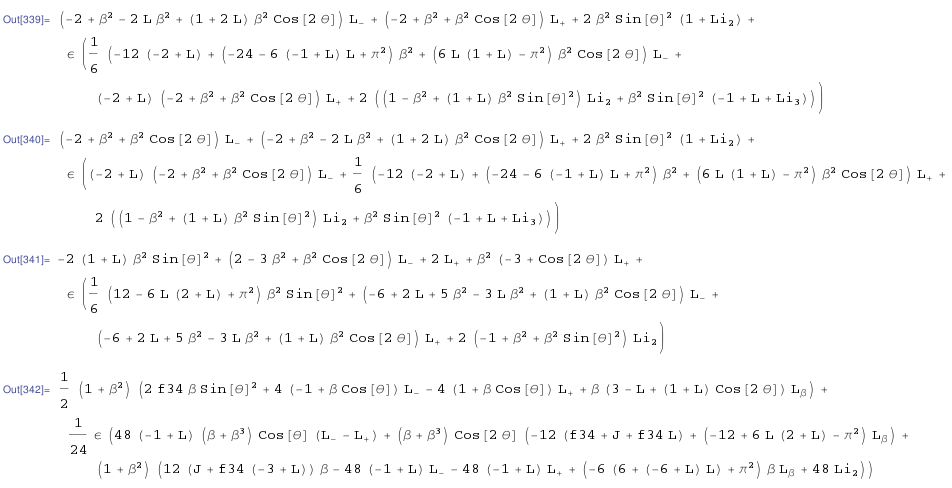
\includegraphics[width=\textwidth]{plots/mixed-soft-function.png}
  \end{center}
  \caption{
   The $C_{jk}$ coefficients of the colour matrices from Eq.~(\ref{eq:
   SMren-res}).
   Notation of Eq.~(\ref{eq:Lplusminu-etc}) expect that $L$ (with no
   subscript) here means $L_\perp$.
  }
  \label{fig:Cjk-coeff}
\end{figure}

%-----------------------------------------------------------------------------
\subsection{Complete $\mathbold{\order{\as^2}}$ mixed contribution }

The NNLO contribution to the differential cross
section~(\ref{eq:factorization-scet}) coming from the mixed term reads
%
\begin{eqnarray}
  \frac{d^4\sigma}{dq_T^2 \, dy \, dM \, d\cos\theta} 
  \bigg |_{\as^2\ \text{mixed}}
  & = &
  \frac{8\pi\beta}{3s M} \frac{1}{2} \int x_Tdx_T \, \, J_0(x_Tq_T) \, \left( \frac{x_T^2M^2}{4e^{-2\gamma_E}} \right)^{-F_{gg}(x_T^2,\mu)}
  \nonumber
  \\
  & & 
  \hspace{40pt} \times \; 4 \frac{3\as^2}{8d_g}\,
  \tr\left[\int \frac{d\phi}{2\pi} [BB\bfH]^{(1)}\bm{W}^{(1)}_{gg} \right]\,,
\end{eqnarray}
%
where the argument of the trace is given in Eq.~(\ref{eq:bbh1wgg1-av}) and we
rewrite here in a slightly different form
%
\begin{eqnarray}
  \int_0^{2\pi} \frac{d\phi}{2\pi}[BB\bfH]^{(1)}\bm{W}^{(1)}_{gg}  & = & 
  %
  \sum_{i,j} \int_{z_1}^{1} \frac{d \xi_1}{\xi_1} 
  \int_{z_2}^{2} \frac{d \xi_2}{\xi_2}
  f_{i/N_1}\left(\frac{z_1}{\xi_1}, \mu\right) 
  f_{j/N_2}\left(\frac{z_2}{\xi_2}, \mu\right)
  %
  \nonumber \\
  & &
  %
  \hspace{-40pt}
  \times \bigg\{
  \frac{1}{4} I_{g\gets i}^{(0)}(\xi_1) I_{g\gets j}^{(0)} (\xi_2)
  \bm{H}^{(1)}_{gg} \bfS_{gg}^{(1)} 
  + \frac{1}{4}
  \Big[
  I_{g\gets i}^{(0)}(\xi_1) \big(I_{g\gets j}^{(1)}(\xi_2) +  
  {I'}_{g\gets j}^{(1)}(\xi_2)\big)
  \nonumber \\
  & &
  + \big(I_{g\gets i}^{(1)}(\xi_1) + 
  {I'}_{g\gets i}^{(1)}(\xi_1) \big) I_{g\gets j}^{(0)}(\xi_2)
  \Big] 
  \bm{H}^{(0)}_{gg}
  \bm{S}^{(1)}_{gg}
  \nonumber 
  \\
  & & 
  \hspace{-20pt}
  + \frac{1}{2 x_T^2}
  \Bigg[
  I_{g\gets i}^{(0)}(\xi_1) {I'}_{g\gets j}^{(1)}(\xi_2)
  +
  {I'}_{g\gets i}^{(1)}(\xi_1) I_{g\gets j}^{(0)}(\xi_2)
  \Bigg]
  \int_0^{2\pi} \frac{d\phi}{2\pi}
  \bm{H}^{M(0)}_{gg}\bm{W}^{(1)}_{gg}
  \bigg\}\,,
  \nonumber \\
  \label{eq:bbh1wgg1-av-rep}
\end{eqnarray}
%
where $I_{g\gets {i}}^{(0)}$ are coefficients which match beam functions into
standard collinear PDFs.

All the quantities are now renormalized.
%
The matching coefficients can be found in~\cite{AntoniaMTh, Becher:2012yn}. The
LO hard function is given by Eq.~(\ref{eq:hard-function-scalar}). The NLO hard
function was computed in~\cite{Ahrens:2011px} and is available in Mathematica
format from the arXiv submission of~\cite{Li:2013mia}.
%
The renormalized average NLO
soft function is given in Eq.~(\ref{eq:soft-function-NLO-ren}) with the colour
matrices collected in Appendix~\ref{app:wmatrices}.
%
Finally the integral from
the last row of the above equation is given in Eq.~(\ref{eq:mixed-integral-av}) with the mixed soft
function given in Eq.~(\ref{eq: SMren-res}) and Fig.~\ref{fig:Cjk-coeff}.



%-----------------------------------------------------------------------------
\chapter{NNLO soft function: general considerations}

\section{Scaling}

Each diagram consists of 


\begin{center}
  {\renewcommand{\arraystretch}{1.0}% for the vertical padding
    \begin{tabular}{cc}
    $d^dk$ & $d$ \\
    $d^dl$ & $d$ \\
    $\delta(k^2)$ & $-2$ \\
    $\delta(l^2)$ & $-2$ \\
    2 $\alpha$ regulators & $-2\alpha$ \\
    transverse delta & $-(d-2)$ \\
    4 quark propagators & $-4$\\
    \hline
    sum: & $d -2 \alpha - 6 = 4-6-2\epsilon - 2\alpha$ \\
         & \hspace{40pt} $= -2 -2\alpha -2\epsilon$
    \end{tabular}
  }
\end{center}

\section{Kinematics}
We need two gluon $d$-vectors
%
\begin{eqnarray}
  k & = & k_{0}\, (1,\ldots,\sin\theta_1\sin\theta_2,
               \sin\theta_1\cos\theta_2,\cos\theta_1)\,, \\
  l & = & l_{0}\, (1,\ldots,\sin\chi_1\sin\chi_2,
               \sin\chi_1\cos\chi_2,\cos\chi_1)\,,
\end{eqnarray}
%
where $\theta_1$ and $\chi_1$ are the polar angles while $\theta_2$ and $\chi_2$
are the azimuthal angles of the gluons.
 
The loop integrals have the form
%
\begin{equation}
  \qquad \qquad \qquad
  \int [dk] [dl]
  \qquad \qquad \qquad \text{where} \qquad  \qquad
  [dk] = d^d k\, \delta(k^2)\, \theta(k^0)\,,
\end{equation}
%
and need to be regularized using the method of Ref.~\cite{Becher:2011dz},
which leads to the replacements
%
\begin{subequations}
   \begin{eqnarray}
     d^d k\, \delta(k^2) \theta(k_0) 
     & \to &
     d^d k \left(\frac{\nu_k}{n \cdot k} \right)^{\alpha}\!
     \delta(k^2)\, \theta(k_0)\,, 
     \\[0.5em]
     d^d l\, \delta(l^2) \theta(l_0) 
     & \to &
     d^d l \left(\frac{\nu_l}{n \cdot l} \right)^{\beta}\!
     \delta(l^2)\, \theta(l_0)\,.
   \end{eqnarray}
   \label{eq:analytic-reg}
\end{subequations}

%-----------------------------------------------------------------------------
\section{Feynman rules for NNLO soft functions}
\label{sec:FRsoft}

In order to understand the Feynman rules we need to remember that the eikonal
vertices come from quark propagators approximated in the soft gluon limit.
%
\begin{itemize}
  \item
  Denominators of the kinetic parts are constructed by going along each quark
  leg $i$ with gluon attachments, assigning momenta as $n_i+k$, $n_i+k+l$ and
  then taking those in eikonal approximation: $n_i \cdot k$, $n_i \cdot (k+l)$,
  etc. 
  %
  Each uncut gluon gets its usual propagator.
  % 
  For example, for the diagram $D_5$ of Fig.~\ref{fig:pecjak2}, that gives $n_i
  \cdot k\, n_i \cdot (k+l)\, n_j \cdot k\, n_j \cdot (k+l)$ while for $D_6$ we
  get $n_i \cdot k\, n_i \cdot (k+l)\, n_j \cdot (k+l) (k+l)^2$.
  \item
  Numerators of the kinetic parts are constructed by simple contractions of
  velocity vectors with corresponding indices.
  %
  \comment{Case of non-abelian diagrams}
  \item
  Colour factors are attributed by starting from the LHS (amplitude) of the cut
  and following gluon attachments along the external lines. 
  %
  Then we move to RHS and follow the lines in the same but put dagger on the
  whole expression, which leads to swapping operators in the final result.
  Three-gluon vertex brings $i f^{abc}$ as usual. Note that the conjugation
  changes the sing of non-abelian amplitudes.
  %
  For example, for diagram $D_5$ of Fig.~\ref{fig:pecjak2} we have 
  $T_i^a T_i^b T_j^b T_j^a$.~\footnote{See my notes for derivation and more
  examples.}
\end{itemize}

%-----------------------------------------------------------------------------
\section{NNLO soft function in position space}

Transformation of the bare NNLO soft function from momentum space to position
space can be schematically written as
%
\begin{align}
  S^{(2)}(L_T) & = 
  \left(f_{-1,0}\, \frac{1}{\epsilon}+ 
  f_{0,1}\, L_T + f_{0,0} + f_{1,2}\, L_T^2\epsilon
  + f_{1,1}\, L_T\epsilon + f_{1,0}\, \epsilon \right)
  \left(s_{-1}\frac{1}{\epsilon} + s_0 + s_1\, \epsilon\right)\,.
\end{align}
%
Hence, the corresponding terms of the position-space soft function read
%
\begin{align}
  S^{(2)}_{-2,0}(L_T) & =  f_{-1,0}\, s_{-1}\, \frac{1}{\epsilon^2}\,,
  \\[0.3em]
  S^{(2)}_{-1,0}(L_T) & =  \left(f_{-1,0}\, s_{0} + f_{0,0}\, s_{-1}\right)\,
                           \frac{1}{\epsilon}\,,
  \\[0.3em]
  S^{(2)}_{-1,1}(L_T) & =  f_{0,1}\, s_{-1} L_T \frac{1}{\epsilon}\,,
  \\[0.3em]
  S^{(2)}_{0,2}(L_T) & =   f_{1,2}\, s_{-1}\, L_T^2\,,
  \\[0.3em]
  S^{(2)}_{0,1}(L_T) & =  \left(f_{0,1}\, s_{0} + f_{1,1}\, s_{-1}\right) L_T\,,
  \\[0.3em]
  S^{(2)}_{0,0}(L_T) & =  \left(f_{-1,0}\, s_{1} + f_{0,0}\, s_{0} +
                                f_{1,0} s_{-1} \right)\,.
  \label{eq:S200}
\end{align}
%
And only the first term in Eq.~(\ref{eq:S200}) needs to be calculated while the
other two can be extracted from RG results for the pole part or for the $L_T$
dependent part.

It is important to note that the finite part of the above object \emph{is not}
equal to the renormalized NNLO soft function one obtains from RG evolution
described in Section~\ref{sec:RGevolution}. The latter includes additional
finite terms coming from pieces like $\tbfS^{(1)}_\bare\bfZ_s^{1}$, as
given in detail in Eq.~(\ref{eq:renS2}).

%-----------------------------------------------------------------------------
\section{Factorization}

Our direct calculation of the bare NNLO soft function and the fact that its pole
structure matches that derived from RGE (real and imaginary part) is a direct
demonstration of small-$q_T$ factorization for this process at this order of
perturbation theory.

%-----------------------------------------------------------------------------
\chapter{NNLO soft function: $\mathbold{n_f}$ part}
%-----------------------------------------------------------------------------

\section{Vacuum polarization integrals}

We consider the process 
%
\begin{equation}
  g(p) \to q(k) + \qbar(p-q)\,.
  %\label{eq:}
\end{equation}

%-----------------------------------------------------------------------------
\subsubsection{Calculation via unitarity}

All propagators are assumed to be defined with $+i\epsilon$ prescription.

\paragraph{Tadpole}
%
The following scalar integral
%
\begin{equation}
  A_0(\alpha_1,\alpha_2) = 
  \int\frac{d^d k}{(n\cdot k)^{\alpha_1}\, (n\cdot (q+k))^{\alpha_2}\, k^2}\,,
  %\label{eq:}
\end{equation}
%
is scaleless and vanishes. To show that, we write
%
\begin{equation}
  %\label{eq:}
  A_0(\alpha_1,\alpha_2)  = 
  \int\frac{d\kp d\km\, k_T^{d-3} dk_T\, d\Omega_{d-3}}
  {k_+^{\alpha_1} (q_++\kp)^{\alpha_2}\, (\kp\km-k_T^2)}\,,
\end{equation}
%
and introduce the rescaling
\begin{equation}
  \km = \lambda\, \km\,, \qquad \qquad
  k_T = \lambda^\frac12\, k_T\,, 
  %\label{eq:}
\end{equation}
%
which leads to
%
\begin{equation}
  %\label{eq:}
  A_0(\alpha_1,\alpha_2)  = 
  \lambda^{1+\frac{d-2}{2}-1} A_0(\alpha_1,\alpha_2)   =
  \lambda^{1-\epsilon} A_0(\alpha_1,\alpha_2)\,. 
\end{equation}

\paragraph{Bubble}

It turns out that the only two-point integral that we need is
%
\begin{equation}
  B_0(\alpha) = 
  \int\frac{d^d k}{(-n\cdot k)^{\alpha}\, (n\cdot (q+k))^{\alpha}\, k^2\,
  (q+k)^2}\,,
  %\label{eq:}
\end{equation}
%
and it can be calculated exactly. After the cut it reads
%
\begin{equation}
  B_0(\alpha) = 
 -2 \pi ^{\frac{d}{2}}\,
  \frac{\Gamma (\epsilon ) \Gamma (1-\alpha -\epsilon )^2 }
  {\Gamma (2-2\alpha -2\epsilon)}\sin (\pi  \epsilon )\,
  q^{-2 \epsilon }\, (n \cdot q)^{-2 \alpha }\,.
  %\label{eq:}
\end{equation}

\paragraph{Vacuum polarization}
%
The self energy tensor has the form
%

\begin{equation}
  \im \Pi^{\mu\nu}(\alpha) = 
  T_{00}\, g^{\mu,\nu} +
  T_{qq}\, q^{\mu}q^{\nu} +
  T_{nn}\, n^{\mu}n^{\nu} +
  T_{qn}\, \left(n^{\mu} q^{\nu}+q^{\mu} n^{\nu}\right)\,
  %\label{eq:}
\end{equation}
%
where
%
\begin{subequations}
  %\label{eq:}
  \begin{align}
  T_{00} &= \frac{2 \left(2 (1-\epsilon)^2-\alpha  (1-2 \epsilon)\right)}
  {(1-\epsilon) (3-2 \alpha -2 \epsilon)}
  \, \calN\, B_0(\alpha)\,
  q^2 
  \,,\\
  %
  T_{qq} &= -\frac{4 (1-\alpha -\epsilon)}{3-2 \alpha -2 \epsilon} 
  \,\calN\, B_0(\alpha)\,,\\
  %
  T_{nn} &= 
  \frac{2 \alpha }{(1-\epsilon) (3-2 \alpha -2 \epsilon)}
  \,\calN\, B_0(\alpha)\,
  \frac{q^4}{\left(n\cdot q\right)^2}
  \,,\\
  %
  T_{qn} &= 
  -\frac{2 \alpha}{(1-\epsilon) (3-2 \alpha -2 \epsilon) }
  \,\calN\, B_0(\alpha)\,
  \frac{q^2}{n\cdot q}
  \,,
  \end{align}
\end{subequations}
%
and
%
\begin{equation}
  \calN = -\frac{g^2}{16} T_F 
  \frac{e^{\epsilon\gamma_E}\mu^{2\epsilon}\nu^{2\alpha}}{\pi^{4-\epsilon}}\,.
  %\label{eq:}
\end{equation}


\section{Soft function integrals}

The above results for the quark bubble can now be embedded into a 2-Wilson-Line
soft function. The integrals have the following general structure
%
\begin{equation}
  I = \int\frac{d^d k\, \delta(k_T^2-1)\, \theta(k^2)\, \theta(k_0)}
      {(n\cdot k)^{a_1+2\alpha} (\nbar\cdot k)^{a_2} (v_3 \cdot k)^{a_3} (v_4
      \cdot k)^{a_4} (k^2)^{a_0+\epsilon}}\,.
  \label{eq:sfnf-general-structure}
\end{equation}
%
What prevents us from direct use of reversed unitarity is the $\theta(k^2)$
function. However, we can trade it for the Dirac delta function at the cost of
introducing extra integration. Namely, we multiply
Eq.~(\ref{eq:sfnf-general-structure}) by 
%
\begin{equation}
  1 = \int_0^\infty dm^2 \delta(k^2-m^2)\,,
  %\label{eq:}
\end{equation}
%
which leads to
\begin{align}
  I & = \int_0^\infty dm^2 \delta(k^2-m^2)
      \int\frac{d^d k\, \delta(k_T^2-1)\, \theta(k^2)\, \theta(k_0)}
      {(n\cdot k)^{a_1+2\alpha} (\nbar\cdot k)^{a_2} (v_3 \cdot k)^{a_3} (v_4
      \cdot k)^{a_4} (k^2)^{a_0+\epsilon}}
    \nonumber \\
    & = \int_0^\infty dm^2 \delta(k^2-m^2)
      \int\frac{d^d k\, \delta(k_T^2-1)\, \theta(m^2)\, \theta(k_0)}
      {(n\cdot k)^{a_1+2\alpha} (\nbar\cdot k)^{a_2} (v_3 \cdot k)^{a_3} (v_4
      \cdot k)^{a_4} (m^2)^{a_0+\epsilon}}
    \nonumber \\
    & = \int_0^\infty dm^2 \frac{\theta(m^2)}{(m^2)^{a_0+\epsilon}}\
      \int\frac{d^d k\, \delta(k_T^2-1)\,\delta(k^2-m^2)  \theta(k_0)}
      {(n\cdot k)^{a_1+2\alpha} (\nbar\cdot k)^{a_2} (v_3 \cdot k)^{a_3} (v_4
      \cdot k)^{a_4}}\,.
  \label{eq:}
\end{align}
%
Hence, we obtain
%
\begin{equation}
  I = \int_0^\infty dm^2 \frac{\theta(m^2)}{(m^2)^{a_0+\epsilon}} \bar I (m^2)\,.
  %\label{eq:}
\end{equation}
%
Now, we can use reversed unitarity to turn delta functions into propagators.
This leads to the following topology
%
\begin{align}
  \label{eq:topology-bubble}
  \bar I(a_1, a_2, a_3, a_4, a_5, a_5)  
  & =   \\ &  \hspace{-30pt}
  \int \frac{d^d k}
  {(n\cdot k)^{a_1+2\alpha} (\nbar\cdot k)^{a_2} (v_3 \cdot k)^{a_3} (v_4
  \cdot k)^{a_4} (k^2-m^2)^{a_5} ((n\cdot k)(\nbar \cdot k)-m^2-1)^{a_6}}\,.
  \nonumber
\end{align}

%-----------------------------------------------------------------------------
\subsection{IBPs}

\begin{enumerate}
  \item
  Standard IBPs:
  \begin{eqnarray}
    \int d^dk\, \frac{\partial}{\partial k^\mu} q^\mu 
    I(a_1,a_2,\ldots, a_{16}) & = & 0\,,
    %\label{eq:}
  \end{eqnarray}
  %
  with $q^\mu = n^\mu, \nbar^\mu, v_3^\mu, v_4^\mu, k^\mu$. This set
  consists of \underline{5 identities}.
  \item
  $q_T$ delta propagator:
  \begin{align}
  I\, \frac{(n\cdot k) (\nbar\cdot k) - m^2-1}
           {(n\cdot k) (\nbar\cdot k) - m^2-1} & = I
  \\[0.5em]
  \text{Ym}[1]\text{Ym}[2]\text{Y}[6] - (m^2+1)\text{Y}[6] & = 1
  \\[0.5em]
  1-\text{Ym}[1]\text{Ym}[2]\text{Y}[6] + (m^2+1)\text{Y}[6] & = 0
  \end{align}
  %
  Hence, we get \underline{1 identity}.
  %
  \item
  Momentum conservation: For $2 \to 3$ kinematics, the exact 4-momenta must
  satisfy
  %
  \begin{equation}
    p_1 + p_2 = p_3 + p_4 + k\,,
    %\label{eq:}
  \end{equation}
  which can be written as
  \begin{equation}
   \frac{M}{2} n + \frac{M}{2} \nbar  = 
   \frac{M}{2} \tilde v_3 + q_3 + \frac{M}{2} \tilde v_4 + q_4 + k\,.
    %\label{eq:}
  \end{equation}
  The above momenta scale as
  %
  \begin{eqnarray}
    n,\, \nbar,\, \tilde v_3,\, \tilde v_4 \sim M (1,1,1)\,, \\
    q_3,\, q_4,\, k \sim M (\lambda, \lambda, \lambda)\,,
    %\label{eq:}
  \end{eqnarray}
  and $q_3$, $q_4$ are constructed such that they balance soft gluon's momentum
  $k$. Hence, $n$, $\nbar$, $\tilde v_3$ and $\tilde v_4$ satisfy the LO, $2\to
  2$ relation
  %
  \begin{equation}
    n + \nbar = \tilde v_3 + \tilde v_4\,.
    %\label{eq:}
  \end{equation}
  Multiplying the above by $k$ leads to the following \underline{1 identity}
  \begin{equation}
    \tilde v_3\cdot k + \tilde v_4\cdot k - n\cdot k  - \nbar\cdot k\,,
    %\label{eq:}
  \end{equation}
  which can be written as
  \begin{equation}
    \text{Ym}[3] + \text{Ym}[4] - \text{Ym}[1] - \text{Ym}[2] = 0\,.
    %\label{eq:}
  \end{equation}
\end{enumerate}

Hence, altogether  we have  7 identities.

%-----------------------------------------------------------------------------
\subsection{Kinematics}
%
Note that the 4-vector $k^\mu$ in Eq.~(\ref{eq:topology-bubble}) is now massive.
Hence, the parametrization from Eq.~(\ref{eq:k4v-par-massless}) does not hold
and it must be replaced with 
%
\begin{equation}
 k  = 
 (k_0, \ldots,
 |\vec k| \sin\theta_1\sin\theta_2, ,|\vec k| \sin\theta_1\cos\theta_2,
 |\vec k| \cos\theta_1)\,,
 \label{eq:k4v-par-massive}
\end{equation}
%
where
%
\begin{equation}
 |\vec k| = \sqrt{k_0^2-m^2}\,.
  %\label{eq:}
\end{equation}
%
Therefore, the relevant inner products now take the form
%
\begin{align}
  n \cdot k & =  k_0 - |\vec k| \cos\theta_1\,, \\
  \nbar \cdot k & =  k_0 + |\vec k| \cos\theta_1\,, \\
  \tilde v_3 \cdot k & =  k_0- 
  \beta\, |\vec k| \sin\theta_1\cos\theta_2\sin\theta -
  \beta\, |\vec k| \cos\theta_1\cos\theta\,, \\
  \tilde v_4 \cdot k & =  k_0+
  \beta\, |\vec k|\sin\theta_1\cos\theta_2\sin\theta +
  \beta\, |\vec k|\cos\theta_1\cos\theta\,.
\end{align}
%
We also get that
%
\begin{align}
 k_0 & = \frac12\left(n\cdot k + \nbar \cdot k\right) \,, \\
 k_0 & = \frac12\left(\tilde v_3\cdot k + \tilde v_4 \cdot k\right)\,.
\end{align}

%-----------------------------------------------------------------------------
\subsection{Derivatives}

\begin{align}
  \frac{d}{d\beta} I & = 
  \left(
  - a_3\, \frac{1}{\tilde v_3 \cdot k}\, \frac{d}{d\beta}(\tilde v_3 \cdot k)  
  - a_4\, \frac{1}{\tilde v_4 \cdot k}\, \frac{d}{d\beta}(\tilde v_4 \cdot k)
  \right)\, I
\end{align}


\begin{align}
  \frac{d}{d\beta}\, \tilde v_3 \cdot k 
  & = 
  - |\vec k| \sin\theta_1\cos\theta_2\sin\theta -
    |\vec k| \cos\theta_1\cos\theta \\
  & = 
  \frac{1}{\beta}\left(\tilde v_3 \cdot k - k_0 \right) \\
  & = 
  \frac{\tilde v_3 \cdot k}{\beta} -
  \frac{n\cdot k}{2\beta} - \frac{\nbar\cdot k}{2\beta} \\
  & = 
  \frac{\tilde v_3 \cdot k}{2\beta} - \frac{\tilde v_4 \cdot k}{2\beta}
\end{align}

\begin{align}
  \frac{d}{d\beta}\, \tilde v_4 \cdot k 
  & = 
    |\vec k| \sin\theta_1\cos\theta_2\sin\theta +
    |\vec k| \cos\theta_1\cos\theta \\
  & = 
  \frac{1}{\beta}\left(\tilde v_4 \cdot k-k_0  \right) \\
  & = 
  \frac{\tilde v_4 \cdot k}{\beta} -
  \frac{n\cdot k}{2\beta} - \frac{\nbar\cdot k}{2\beta} \\
  & = 
  \frac{\tilde v_4 \cdot k}{2\beta} - \frac{\tilde v_3 \cdot k}{2\beta}
\end{align}

The above results allow one to write down the general formula for derivative of
the topology~(\ref{eq:topology-bubble})
%
\begin{equation}
  \frac{d}{d\beta} = 
  -\frac{1}{2\beta}\left\{
  a_3 \left(1-\frac{\tilde v_4 \cdot k}{\tilde v_3 \cdot k}\right) +
  a_4 \left(1-\frac{\tilde v_3 \cdot k}{\tilde v_4 \cdot k}\right)
  \right\}\,.
  %\label{eq:}
\end{equation}


%-----------------------------------------------------------------------------
\chapter{NNLO soft function: real-virtual}

%-----------------------------------------------------------------------------
\section{Soft currents}

Following Ref.~\cite{Bierenbaum:2011gg} we introduce the tree level and (UV-renormalized) one-loop soft currents
%
\begin{align}
  J_a^{\mu (0)} & = \sum_{i=1}^n T_i^a e_i^\mu\,,
  \\
  J_a^{\mu (1)} & = i f^{abc} \sum_{i\neq j=1}^n T_i^b T_j^c 
                    \left(e_i^\mu-e_j^\mu\right) 
		    g_{ij}^{(1)}(\epsilon,q, p_i, p_j)\,,
\end{align}
%
where
%
\begin{equation}
  %\label{eq:}
  e_i^\mu = \frac{p_i^\mu}{p_i \cdot q}\,,
\end{equation}
%
and the function $g_{ij}$ is symmetric under the exchange $i\leftrightarrow j$.

%-----------------------------------------------------------------------------
\section{Diagrams of the type 123}

\begin{figure}[t]
  \begin{center}
    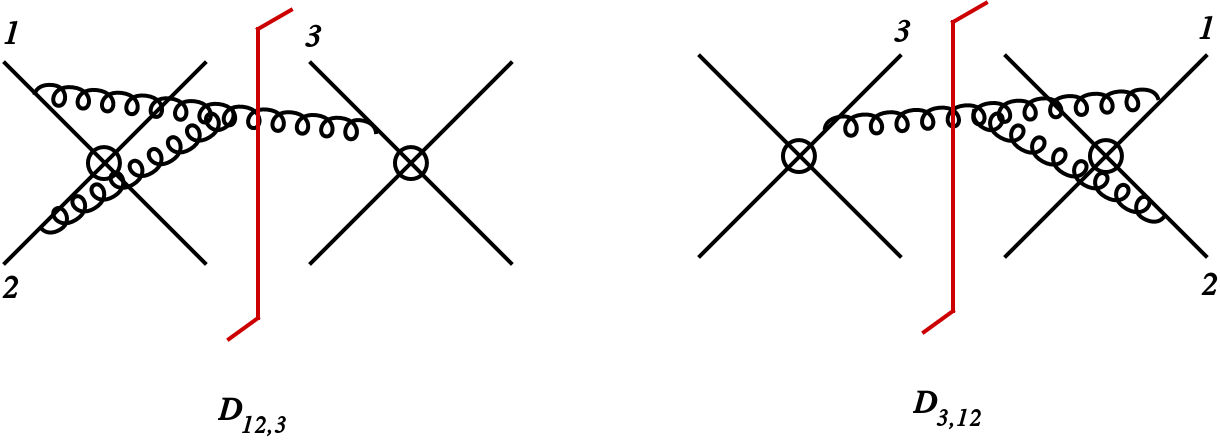
\includegraphics[width=0.80\textwidth]{plots/sf-nnlo-1cut123.png}
  \end{center}
  \caption{
  }
  \label{fig:diag123}
\end{figure}

Let us consider a special case of 3-Wilson-line diagrams which involve two
massless and one massive particle. Two such diagrams are depicted in
Fig.~\ref{fig:diag123}.

Using the notation introduced above we can write expressions corresponding to
those two diagrams
%
\begin{align}
  D_{12,3} & = i f^{abc}\, T_3^a T_1^b T_2^c\, 
             \left(e_1^\mu-e_2^\mu\right) e_3^\mu\, g_{12}^{(1)}\,,
  \\[0.5em]
  D_{3,12} & = -i f^{abc}\, T_3^a T_1^b T_2^c\, 
             \left(e_1^\mu-e_2^\mu\right) e_3^\mu\, g_{12}^{(1)\,*}\,.
\end{align}
%
Hence, their sum reads
%
\begin{equation}
  D_{12,3}  + D_{3,12}  = i f^{abc}\, T_3^a T_1^b T_2^c\, 
                          \left(e_1^\mu-e_2^\mu\right) e_3^\mu\,
	                  \left(g_{12}^{(1)}-g_{12}^{(1)\,*}\right)\,.
  %\label{eq:}
\end{equation}

We see that the result is purely imaginary and that it does not vanish as the
antisymmetry of the colour factor under the exchange $1 \leftrightarrow 2$ is
compensated by the antisymmetry of the kinematic part.

This is in contradiction with the claims made in Ref.~\cite{Becher:2009qa} where
it is argued that all three-particle structures with two massless and one
massive Wilson lines must vanish. This conclusion, however, follows from the
constraint imposed on the form of the anomalous dimension which is a consequence
of factorization. Yet, the latter is not proven anywhere in the discussion but
it is only assumed.

%------------------------------------
\subsection*{Scaling}

The soft current for massless particles with momenta $p_{1,2} = (1,0,0,\pm 1)$
reads~\cite{Catani:2000pi}
%
\begin{align}
  J_{2P}^{a(1)}(p_1,p_2;q, \epsilon) & = 
  -\frac{1}{16\pi^2}  i f_{abc} T_1^b T_2^c\, \epsilon_\mu(q)
  \left(\frac{p_1^\mu}{p_1\cdot q}- \frac{p_2^\mu}{p_2\cdot q}\right)
  \nonumber \\
  & \times
  \left(\frac{4\pi p_1\cdot p_2}{2 p_1 \cdot q\, p_2 \cdot q e^{-i\pi}}
  \right)^\epsilon
  \frac{1}{\epsilon^2}
  \frac{\Gamma^3(1-\epsilon)\Gamma^2(1+\epsilon)}{\Gamma(1-2\epsilon)}\,.
\end{align}
%
Embedding the above in the integral over $q$ gives
%
\begin{align}
  G_{12,3} & \propto i f_{abc} T_3^a T_1^b T_2^c\,
  \frac{1}{\epsilon^2}\,
  \frac{\Gamma^3(1-\epsilon)\Gamma^2(1+\epsilon)}{\Gamma(1-2\epsilon)}
  \nonumber \\
  & \times
  \int d^d q\,
  \frac{\delta^+(q^2)\delta^{(2)}(q_\perp-1)}
       {q_+ p_{3-}+q_- p_{3+}-q_\perp \cdot p_{3\perp}}\,
  \frac{1}{q_+^\alpha}
  \left(\frac{p_{3+}}{q_+}- \frac{p_{3-}}{q_-}\right)
  \left(\frac{4\pi}{q_+\, q_-\, e^{-i\pi}}
  \right)^\epsilon.
\end{align}
%
Let us now apply the change of variables, motivated by Ref.~\cite{Aybat:2006wq}
%
\begin{equation}
  (q_+,q_-,q_\perp) \to (\xi q_-,\xi^{-1} q_+,q_\perp)
  \qquad
  \text{with} 
  \quad
  \xi = p_{3+}/p_{3-}\,.
  \quad
  %\label{eq:}
\end{equation}
%
Our integral becomes
%
\begin{align}
  G_{12,3} (\alpha) & \propto i f_{abc}  T_3^a T_1^b T_2^c \,
  \frac{1}{\epsilon^2}\,
  \frac{\Gamma^3(1-\epsilon)\Gamma^2(1+\epsilon)}{\Gamma(1-2\epsilon)}
  \nonumber \\
  & \times
  \int d^d q\, 
  \frac{\delta^+(q^2)\delta^{(2)}(q_\perp-1)}
       {q_+ p_{3-}+q_- p_{3+}-q_\perp \cdot
  p_{3\perp}}
  \xi^{-\alpha}\frac{1}{q_-^\alpha}
  \left(\frac{p_{3-}}{q_-} - \frac{p_{3+}}{q_+}\right)
  \left(\frac{4\pi}{q_+\, q_-\, e^{-i\pi}}
  \right)^\epsilon
  \nonumber \\
  & = - \xi^{-\alpha} G_{12,3}(-\alpha)\,.
\end{align}
%
Hence, we see that the above integral would exhibit scaling and vanish if only
there was no $\alpha$ regulator. However, without the regulator, the integral is
divergent. Hence, we conclude that the tree-particle graph with two massless and
one massive Wilson lines does not vanish.

A few comments are in order:
%
\begin{enumerate}
  \item
  The above result will only affect the imaginary part of the soft function. The
  tree-particle graphs of the type of 123 will not contribute to the soft
  function as there will always be a complex-conjugate diagram with opposite
  sign due to colour operator.
  \item
  The above result does not invalidate the analysis of Ref.~\cite{Aybat:2006wq},
  where it is claimed that the massless-massless-massive diagrams vanish because
  of certain scaling properties. The key difference between our case and the one
  discussed there is that in Ref.~\cite{Aybat:2006wq} purely virtual diagrams
  are consider. And in those diagrams, rapidity divergences are regularized by
  dimensional regularization~\cite{Becher:2011dz}.  Hence, no $\alpha$ regulator
  is required and the scaling holds.
  \item
  The key element of our calculation, which prevents the diagram 123 from
  vanishing, is the transverse delta function. As explained in
  Ref.~\cite{Becher:2011dz} without this function, integration over the
  transverse momentum provides a factor $k_-^{-\epsilon}$ which regularizes
  rapidity divergences. However, when the transverse delta is present it fixes
  $q_\perp$ to some external value and the integration of $q_\perp$ does
  provide a regular of light-cone singularities. Hence, we need to introduce
  $\alpha$.
\end{enumerate}

%-----------------------------------------------------------------------------
\chapter{NNLO soft function: double real}
\section{Double-real NNLO integrals}

At NNLO, we have two gluons which connect the Wilson lines in various ways.
Ref.~\cite{Ferroglia:2012uy} distinguishes the following types of integrals: 
%
\begin{itemize}
  \item
   \emph{two-Wilson-line integrals}: two gluons connect only two types
   of Wilson lines $i$ and $j$,
  \item
   \emph{three-Wilson-line integrals}: two gluons connect three types
   of Wilson lines $i$, $j$ and $k$,
  \item
   \emph{four-Wilson-line integrals}: two gluons connect four types of
   Wilson lines $i$, $j$, $k$ and $l$.
\end{itemize}

The relevant integrals can be deduced from Ref.~\cite{Ferroglia:2012uy}, where,
however, fully massless case in the threshold limit is considered. Our \ttbar
production requires the following modifications of the original formulae:
%
\begin{itemize}
  \item
  The delta functions get the replacement:
  $\delta(\omega - n_0 \cdot (k+l)) \to \delta^{(2)}(q_\perp-k_\perp-l_\perp)$,
  which comes from replacing the threshold limit by the soft limit.
  \item
  Integrals are regularized according to Eqs.~(\ref{eq:analytic-reg}).
\end{itemize}

In the following subsections, we shall present the formulae for two-, three- and
four-Wilson-line integrals. For better readability, we will skip the common
factor
%
\begin{equation}
  \Sigma' = v_k^\alpha v_l^\beta\,,
  %\label{eq:}
\end{equation}
%
which shall be restored at the end of the calculation.~\footnote{The above needs
to be adjusted further with $\msbar$ related factors etc.}

%-----------------------------------------------------------------------------
\subsubsection{Two-Wilson-line integrals}

\begin{figure}[t]
  \begin{center}
    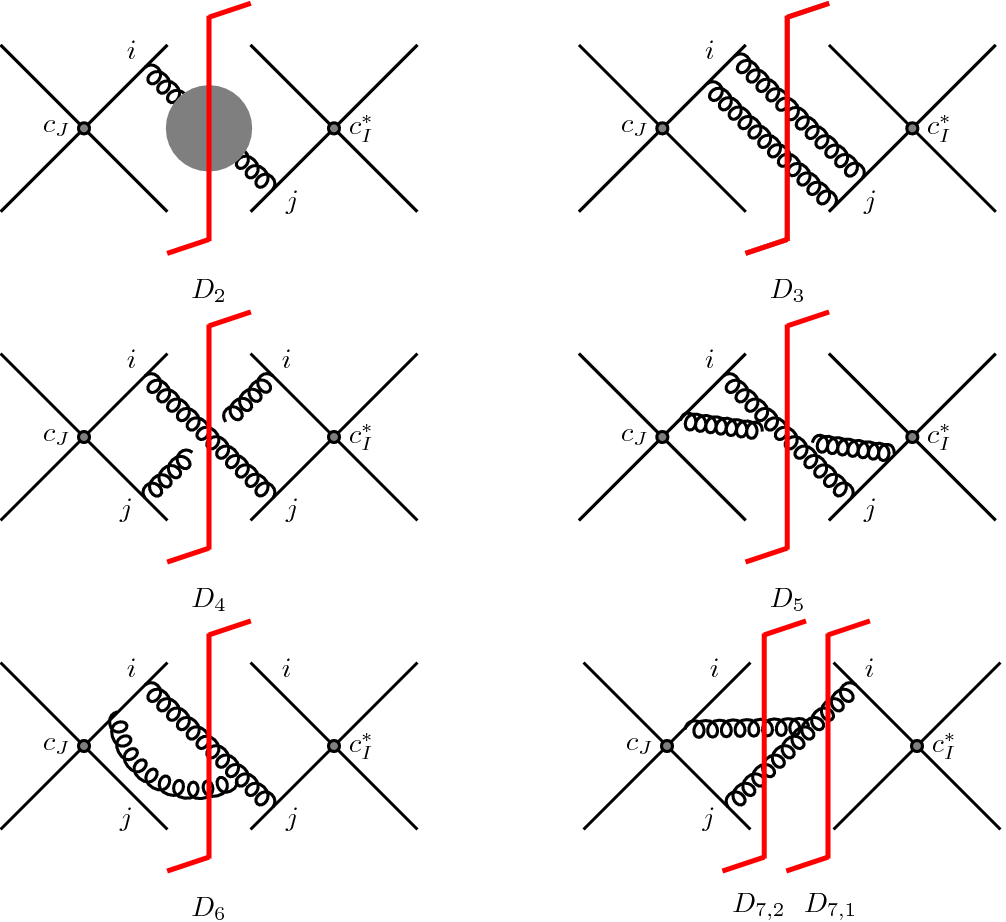
\includegraphics[width=0.7\textwidth]{plots/diagram2-pecjak.png}
  \end{center}
  \caption{Two-Wilson-line integrals for the soft function in the massless case.
  Figure from~\cite{Ferroglia:2012uy}. Our expressions for \ttbar production
  correspond to diagrams with the gluons attached to both initial
  (massless) and final (massive) Wilson lines.}
  \label{fig:pecjak2}
\end{figure}

The relevant integrals correspond to diagrams of Fig.~\ref{fig:pecjak2}, taken
from Ref. ~\cite{Ferroglia:2012uy}. 
%
The expressions read
%
\begin{subequations}
  \label{eq:2WLIset}
  \begin{align}
    %%%
    I_{3, ij} &= 
    (n_i \cdot n_j)^2
    \int d^d k\, d^d l\; 
    \frac{\delta_+(k^2) \, \delta_+(l^2)\,
      \; \delta^{(2)}(q_\perp-k_\perp-l_\perp)}
      {(n \cdot k)^\alpha\; (n \cdot l)^\beta \; 
      n_i \cdot k \; n_i \cdot
      (k+l) \; n_j \cdot l \; n_j \cdot (k+l)} \, ,
    \\[0.7em]
    %%%
    I_{4, ij} &= 
    (n_i \cdot n_j)^2
    \int d^d k\, d^d l\; 
    \frac{\delta_+(k^2) \, \delta_+(l^2) \,
      \; \delta^{(2)}(q_\perp-k_\perp-l_\perp)}
      {(n \cdot k)^\alpha\; (n \cdot l)^\beta \;
      n_i \cdot k \; n_i \cdot l \;
      n_j \cdot k \; n_j \cdot l} \, ,
    \\[0.7em]
    %%%
    I_{5, ij} &=
    (n_i \cdot n_j)^2
    \int d^d k\, d^d l\; 
    \frac{\delta_+(k^2) \, \delta_+(l^2) \,
      \; \delta^{(2)}(q_\perp-k_\perp-l_\perp)}
      {(n \cdot k)^\alpha\; (n \cdot l)^\beta  \;
      n_i \cdot k \; n_i \cdot
      (k+l) \; n_j \cdot k \; n_j \cdot (k+l)} \, , 
    \\[0.7em]
    %%%
    \label{eq:I6ij}
    I_{6,ij} &=
    n_i \cdot n_j
    \int d^d k\, d^d l\; 
    \frac{n_i \cdot (l-k) \;\delta_+(k^2) \, \delta_+(l^2) \, 
     \delta^{(2)}(q_\perp-k_\perp-l_\perp)}
      {(n \cdot k)^\alpha\; (n \cdot l)^\beta  \;
      n_i \cdot k \; n_i \cdot (k+l) \; n_j \cdot (k+l) \; (k+l)^2} \, , 
    \\[0.7em]
    %%%
    \label{eq:I72ij}
    I_{7,2, ij} &=
    n_i \cdot n_j
    \int d^d k\, d^d l\; 
    \frac{n_j \cdot (k+2l) \; \delta_+(k^2) \, \delta_+(l^2) \,
      \delta^{(2)}(q_\perp-k_\perp-l_\perp)}
      {(n \cdot k)^\alpha\; (n \cdot l)^\beta  \;
      n_i \cdot k \; n_j \cdot (k+l) \; n_j \cdot l \; (k+l)^2} \, .
  \end{align}
\end{subequations}
%
where
\begin{equation}
  n_1 = n,     \qquad \qquad
  n_2 = \nbar, \qquad \qquad
  n_3 = \tilde v_3,   \qquad \qquad
  n_4 = \tilde v_4\,.
  \label{eq:nnlo-external-particles}
\end{equation}
%
We note that the above integrals are invariant under rescaling of external
momenta. This will be also true for three- and four-Wilson-line integrals.
Hence, we can work with $v_{3,4}$ or $\tilde v_{3,4}$. We choose the latter as
it leads to more compact expressions.
 
For the time being, we put aside $I_{2, ij}$ and 
$I_{7,1, ij}$ as they are effectively expressible in terms of 1-loop integrals.
These cases will be discussed in next section.

In the massless case, all diagonal terms vanish, as they are proportional to
$n_i^2 = 0$. (This originates from the use of dimensional regularization in
which scaleless integrals are zero.) In \ttbar production, this is certainly true
for the incoming particles, hence for $i=1,2$, whereas the other two diagonal
integrals with $i=3,4$ are in general non-zero.~\footnote{
There are certainly other symmetries between those integrals, which we can
study later.
%
In particular, there is a chance that, since we adopted the analytic regularization scheme
of~\cite{Li:2013mia}, the integrals $I_{12}$ and $I_{21}$ are also
scaleless and vanish as well~(see~\cite{Becher:2010tm}). 
%
This was true at NLO but here would need to be checked directly. For the time
being, we assume that those integrals do not vanish.
%
BTW, the integrals $I_{12}$ and $I_{21}$
do not vanish in the threshold limit~\cite{Ahrens:2010zv}, where the delta
function breaks scalelessness, or in the soft limit with a different
regularization scheme, as
in~\cite{Chiu:2012ir}. Both of the above calculations render non-vanishing
soft functions with non-diagonal initial-initial connections. 
%
As mentioned in~\cite{Li:2013mia}, vanishing of  $I_{12 (21)}$ integrals in
certain scheme does not break scheme-independence as those integrals can be
absorbed into collinear sectors~\cite{Li:2013mia}, hence disappear, in any
scheme.
}
%
More specifically, the five sets of integrals given in Eqs.~(\ref{eq:2WLIset})
have the following structure
%
\begin{subequations}
  \begin{align}
    I_{3, ij},\ I_{5, ij},\ I_{6, ij} &= 
    \left(
    \begin{array}{cccc}
    0      & I_{12} & I_{13} & I_{14} \\
    I_{21} & 0      & I_{23} & I_{24} \\
    I_{31} & I_{32} & I_{33} & I_{34} \\
    I_{41} & I_{42} & I_{43} & I_{44} 
    \end{array}
    \right)\,,
    \\[0.7em]
    %%%
    I_{4, ij},\ I_{7,2, ij} &= 
    \left(
    \begin{array}{cccc}
    0      & I_{12} & I_{13} & I_{14} \\
    I_{21} & 0      & I_{23} & I_{24} \\
    I_{31} & I_{32} & 0      & I_{34} \\
    I_{41} & I_{42} & I_{43} & 0 
    \end{array}
    \right)\,.
  \end{align}
  %\label{eq:}
\end{subequations}
 
Vanishing of $I_{11}$ and $I_{22}$ has been explained above. The reason why there
are no $I_{33}$ and $I_{44}$ integrals in the second matrix is clear by looking
at the corresponding diagrams in Fig.~\ref{fig:pecjak2}. 

Setting $i=j$ in $D_4$ or $D_{7,2}$ would turn them into $D_5$ and $D_6$,
respectively. But the corresponding expressions from Eqs.~(\ref{eq:2WLIset})
would be wrong since, \eg $D_4$ corresponds to a product of four different
Wilson lines, expanded to order $g_s$, whereas $D_5$ represents two Wilson
lines, each expanded to order $g_s^2$. So, the diagonal expressions for
$I_{4, ij}$ and $I_{7,2, ij}$ simply make no sense and should not be calculated.
%
Another way to see this is by noticing that $D_4$ is in fact a convolution of
two NLO soft functions as none of the momenta attaches to the same
line twice.



%-----------------------------------------------------------------------------
\subsubsection{Three-Wilson-line integrals}


From Fig.~\ref{fig:pecjak3} and the Feynman rules of sec.~\ref{sec:FRsoft} we
deduce the following integrals~\cite{Ferroglia:2012uy} 
%
\begin{subequations}
  \label{eq:3WLIset}
  \begin{align}
    %%%
    I_{8, ijk}^{(a)+(b)} &= 
    n_i \cdot n_j\; n_i \cdot n_k\; 
    \int d^d k\, d^d l\; 
    \frac{\delta_+(k^2) \, \delta_+(l^2)\,
      \; \delta^{(2)}(q_\perp-k_\perp-l_\perp)}
      {(n \cdot k)^\alpha\; (n \cdot l)^\beta \; 
      n_i \cdot k \; n_i \cdot l \; n_j \cdot k \; n_k \cdot l} \, ,
    \\[0.7em]
    %%%
    I_{8, ijk}^{(c)+(d)} &= 
    n_i \cdot n_j\; n_i \cdot n_k\; 
    \int d^d k\, d^d l\; 
    \frac{\delta_+(k^2) \, \delta_+(l^2)\,
      \; \delta^{(2)}(q_\perp-k_\perp-l_\perp)}
      {(n \cdot k)^\alpha\; (n \cdot l)^\beta \; 
      n_i \cdot l \; n_i \cdot (k+l) \; n_j \cdot k \; n_k \cdot l} \, ,
    \\[0.7em]
    %%%
    I_{8, ijk}^{(e)+(f)} &= 
    n_i \cdot n_j\; n_i \cdot n_k\; 
    \int d^d k\, d^d l\; 
    \frac{\delta_+(k^2) \, \delta_+(l^2)\,
      \; \delta^{(2)}(q_\perp-k_\perp-l_\perp)}
      {(n \cdot k)^\alpha\; (n \cdot l)^\beta \; 
      n_i \cdot k \; n_i \cdot (k+l) \; n_j \cdot k \; n_k \cdot l} \,,
  \end{align}
\end{subequations}
%
and the external particles are defined as in
Eq.~(\ref{eq:nnlo-external-particles}).
%
Each of the above integrals is proportional to a different colour factor.

\begin{figure}[t]
  \begin{center}
    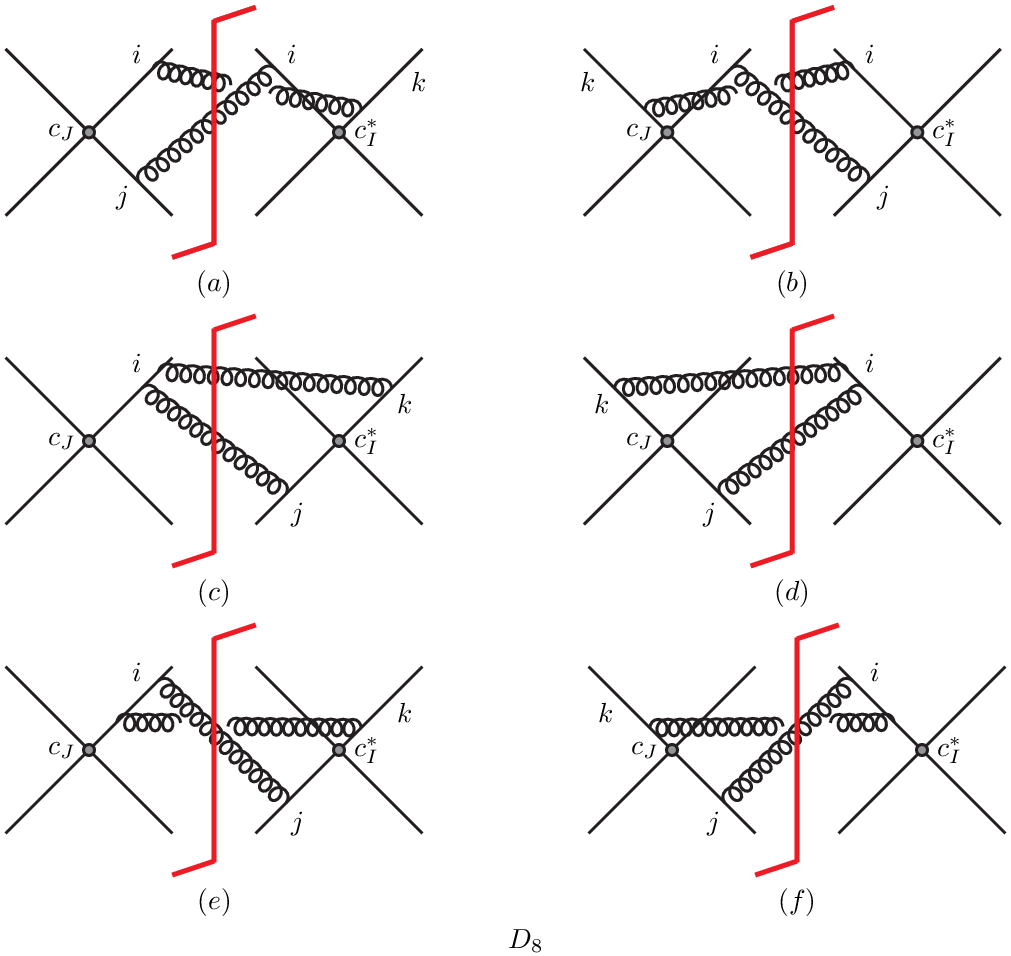
\includegraphics[width=0.7\textwidth]{plots/diagram3-pecjak.png}
  \end{center}
  \caption{
    Three-Wilson-line integrals, the abelian case.
  }
  \label{fig:pecjak3}
\end{figure}
%
\begin{figure}[t]
  \begin{center}
    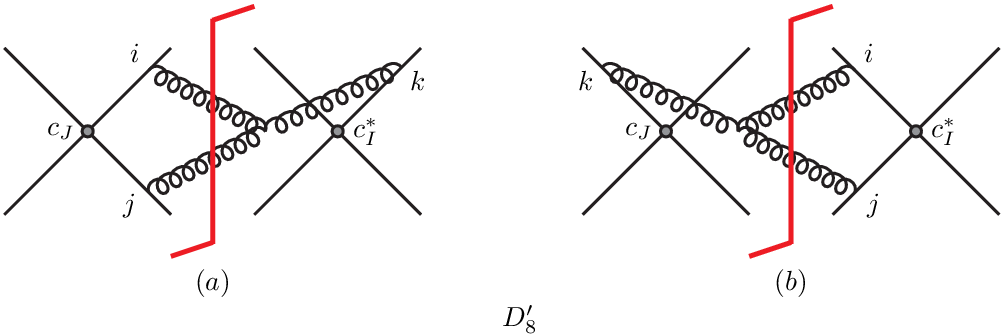
\includegraphics[width=0.7\textwidth]{plots/diagram5-pecjak.png}
  \end{center}
  \caption{
    Three-Wilson-line integrals, the non-abelian case.
  }
  \label{fig:pecjak5}
\end{figure}

Diagrams $(a)$ and $(b)$ are again convolutions of NLO soft functions, hence we
set all the diagonal terms: $I_{iik}, I_{iji}, I_{ijj}$ to zero. 
%
As for $(c), (d), (e)$ and $(f)$, we may have $I_{iik}, I_{iji}$ but not
$I_{ijj}$, as the latter would involve only two Wilson lines. Of the first two,
the integrals do not vanish only if $i=3,4$. In summary, the three-Wilson-lines
integrals given in Eqs.~(\ref{eq:3WLIset}) and represented by diagrams in
Fig.~\ref{fig:pecjak3} are non-vanishing except for
%
\begin{equation}
  \begin{array}{ccc}
  I^{(a,b)}_{8,ijk} = 0     & \quad \text{if} \quad & 
                               i=j\ \lor\ i=k\ \lor\ j=k\,,
  \\[0.5em]
  I^{(c,d,e,f)}_{8,ijk} = 0 & \quad \text{if} \quad & j=k\,,
  \\[0.5em]
  I^{(c,d,e,f)}_{8,ijk} = 0 & \quad \text{if} \quad & 
                              (i=j\ \lor\ i=k)\ \land\ (i=1\ \lor\ i=2)\,.
  \end{array}
  %\label{eq:}
\end{equation}

There is also a group of non-abelian integrals like those shown in
Fig.~\ref{fig:pecjak5}. The sum of those two diagrams vanishes due to colour
structure as, following the Feynman rules discussed earlier, we have
%
\begin{subequations}
  \begin{align}
   D'^{(a)}_8 &\propto i f^{abc}\, T_i^a\, T_j^b\, T_k^c\, I'_8\,, \\
   D'^{(b)}_8 &\propto -i f^{abc}\, T_i^a\, T_j^b\, T_k^c\, I'_8\,.
  \end{align}
  %\label{eq:}
\end{subequations}
%
The relative minus sign comes from the fact that the gluon propagator carrying
momentum $k+l$ appears on opposite sides of the cut in the two diagrams
(see sec.~3.2 in ~\cite{Ferroglia:2012uy} for further discussion).
%
The same is true for one-particle cut diagrams analogous to those of
Fig.~\ref{fig:pecjak5}.



%-----------------------------------------------------------------------------
\subsubsection{Four-Wilson-line integrals}
 
\begin{figure}[t]
  \begin{center}
    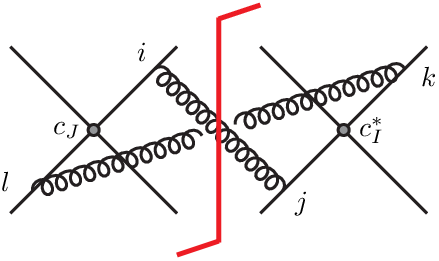
\includegraphics[width=0.35\textwidth]{plots/diagram6-pecjak.png}
  \end{center}
  \caption{
    Four-Wilson-line integrals.
  }
  \label{fig:pecjak6}
\end{figure}

Finally, we have the integrals corresponding to Fig.~\ref{fig:pecjak6}, with 
four different gluon attachments~\cite{Ferroglia:2012uy}
%
\begin{align}
  %%%
  \label{eq:4WLIset}
  I_{9, ijkl} &= 
  n_i \cdot n_j\; n_k \cdot n_l\; 
  \int d^d k\, d^d l\; 
  \frac{\delta_+(k^2) \, \delta_+(l^2)\,
    \; \delta^{(2)}(q_\perp-k_\perp-l_\perp)}
    {(n \cdot k)^\alpha\; (n \cdot l)^\beta \; 
    n_i \cdot k \; n_j \cdot k \; n_k \cdot l \; n_l \cdot l} \,.
\end{align}

Some of the indices have a chance to be equal and render the integral non-zero
provided that the gluons are attached to four distinct Wilson lines and, as
usual, only the squares of massive vectors, hence $n_i^2$ with $i=3,4$, survive.
On the other hand, if the two indices on the same side of the cut become equal,
that corresponds to three-Wilson-lines diagram and should be rejected.
We can summarize the above by
%
\begin{equation}
  \begin{array}{ccc}
  I_{9, ijkl} = 0  &\quad \text{if} \quad & (i=j\ \land\ i = 1,2)\ \lor\
                                            (k=l\ \land\ k = 1,2)\,,
  \\[0.5em]
  I_{9, ijkl} = 0  &\quad \text{if} \quad & i=l\ \lor\ k=j\,.
  \end{array}
  %\label{eq:}
\end{equation}

%------------------------------------
\section{General form of NNLO integral}

We would like to write all the above cases of two-, three- and four-Wilson-line
integrals, given in Eqs.~(\ref{eq:2WLIset}), (\ref{eq:3WLIset})
and~(\ref{eq:4WLIset}), as a single topology. 
%
Because of the argument of the $\delta^{(2)}(q_\perp-k_\perp-l_\perp)$ function,
it is useful to change variables according to
%
\begin{subequations}
\begin{align}
  k &= k\,,  \\
  p &= k+l \quad \to \quad l = p-k\,, 
  \label{eq:p-def}
\end{align}
\end{subequations}
%
which, similarly to the NLO case, allows one to write
%
\begin{equation}
  \delta^{(2)}(q_\perp-k_\perp-l_\perp) = 2 \delta(p_T^2-q_T^2) \delta(\phi)\,,
  %\label{eq:}
\end{equation}
%
where $\phi$ is the azimuthal angle of $p_\perp$ and the azimuthal integral
can be performed trivially.

Then, we notice that $I_{6,ij}$ and $I_{7,2,ij}$, given in Eqs.~(\ref{eq:I6ij})
and~(\ref{eq:I72ij}), can be split such that
%
\begin{eqnarray}
  I_{6,ij} & = & I^{(a)}_{6,ij} - 2 I^{(b)}_{6,ij}\,, \\
  I_{7,2,ij} & = &  I^{(a)}_{7,2,ij} + I^{(b)}_{7,2,ij}\,,
  %\label{eq:}
\end{eqnarray}
%
with the integrals on the RHS involving only three denominators and no
propagator in the numerator.

The full set of integrals which need to be calculated reads 
%
\begin{subequations}
  \label{eq:fullset}
  \begin{align}
    %%%
    I_{3, ij} &= 
    (n_i \cdot n_j)^2
    \int 
    \frac{d^d k\, d^d p\;\delta_+(k^2)\, \delta_+((p-k)^2)\,\delta(p_T^2-q_T^2)}
      {(n \cdot k)^\alpha\; (n \cdot [p-k])^\beta \; 
      (n_i \cdot k) \; (n_i \cdot p) \; (n_j \cdot [p-k]) \; (n_j \cdot p)} \, ,
    \\[0.7em]
    %%%
    I_{4, ij} &= 
    (n_i \cdot n_j)^2
    \int 
    \frac{d^d k\, d^d p\;\delta_+(k^2)\, \delta_+((p-k)^2)\,\delta(p_T^2-q_T^2)}
      {(n \cdot k)^\alpha\; (n \cdot [p-k])^\beta \;
      (n_i \cdot k) \; (n_i \cdot [p-k]) \;
      (n_j \cdot k) \; (n_j \cdot [p-k])} \, ,
    \\[0.7em]
    %%%
    I_{5, ij} &=
    (n_i \cdot n_j)^2
    \int 
    \frac{d^d k\, d^d p\;\delta_+(k^2)\, \delta_+((p-k)^2)\,\delta(p_T^2-q_T^2)}
      {(n \cdot k)^\alpha\; (n \cdot [p-k])^\beta  \;
      (n_i \cdot k) \; (n_i \cdot p) \; 
      (n_j \cdot k) \; (n_j \cdot p)} \, , 
    \\[0.7em]
    %%%
    I^{(a)}_{6,ij} &=
    n_i \cdot n_j
     \int 
    \frac{d^d k\, d^d p\;\delta_+(k^2)\, \delta_+((p-k)^2)\,\delta(p_T^2-q_T^2)}
      {(n \cdot k)^\alpha\; (n \cdot [p-k])^\beta  \;
      (n_i \cdot k) \; (n_j \cdot p) \; p^2} \, , 
    \\[0.7em]
    %%%
    I^{(b)}_{6,ij} &=
    n_i \cdot n_j
    \int 
    \frac{d^d k\, d^d p\;\delta_+(k^2)\, \delta_+((p-k)^2)\,\delta(p_T^2-q_T^2)}
      {(n \cdot k)^\alpha\; (n \cdot [p-k])^\beta  \;
      (n_i \cdot p) \; (n_j \cdot p) \; p^2} \, , 
    \\[0.7em]
    %%%
    I^{(a)}_{7,2, ij} &=
    n_i \cdot n_j
    \int 
    \frac{d^d k\, d^d p\;\delta_+(k^2)\, \delta_+((p-k)^2)\,\delta(p_T^2-q_T^2)}
      {(n \cdot k)^\alpha\; (n \cdot [p-k])^\beta  \;
      (n_i \cdot k) \;  (n_j \cdot [p-k]) \; p^2} \, ,
    \\[0.7em]
    %%%
    I^{(b)}_{7,2, ij} &=
    n_i \cdot n_j
    \int 
    \frac{d^d k\, d^d p\;\delta_+(k^2)\, \delta_+((p-k)^2)\,\delta(p_T^2-q_T^2)}
      {(n \cdot k)^\alpha\; (n \cdot [p-k])^\beta  \;
      (n_i \cdot k) \; (n_j \cdot p) \; p^2} = I^{(a)}_{6,ij}\, ,
    \\[0.7em]
    %%%
    I_{8, ijk}^{(a)+(b)} &= 
    n_i \cdot n_j\; n_i \cdot n_k\; 
    \int 
    \frac{d^d k\, d^d p\;\delta_+(k^2)\, \delta_+((p-k)^2)\,\delta(p_T^2-q_T^2)}
      {(n \cdot k)^\alpha\; (n \cdot [p-k])^\beta \; 
      (n_i \cdot k) \; (n_i \cdot [p-k]) \; 
      (n_j \cdot k) \; (n_k \cdot [p-k])} \, ,
    \\[0.7em]
    %%%
    I_{8, ijk}^{(c)+(d)} &= 
    n_i \cdot n_j\; n_i \cdot n_k\; 
    \int 
    \frac{d^d k\, d^d p\;\delta_+(k^2)\, \delta_+((p-k)^2)\,\delta(p_T^2-q_T^2)}
      {(n \cdot k)^\alpha\; (n \cdot [p-k])^\beta \; 
      (n_i \cdot [p-k]) \; (n_i \cdot p) \; 
      (n_j \cdot k) \; (n_k \cdot [p-k])} \, ,
    \\[0.7em]
    %%%
    I_{8, ijk}^{(e)+(f)} &= 
    n_i \cdot n_j\; n_i \cdot n_k\; 
    \int 
    \frac{d^d k\, d^d p\;\delta_+(k^2)\, \delta_+((p-k)^2)\,\delta(p_T^2-q_T^2)}
      {(n \cdot k)^\alpha\; (n \cdot [p-k])^\beta \; 
      (n_i \cdot k) \; (n_i \cdot p) \; (n_j \cdot k) \; (n_k \cdot [p-k])} \,,
    \\[0.7em]
    %%%
    I_{9, ijkl} &= 
    n_i \cdot n_j\; n_k \cdot n_l\; 
    \int 
    \frac{d^d k\, d^d p\;\delta_+(k^2)\, \delta_+((p-k)^2)\,\delta(p_T^2-q_T^2)}
      {(n \cdot k)^\alpha\; (n \cdot [p-k])^\beta \; 
      (n_i \cdot k) \; (n_j \cdot k) \; (n_k \cdot [p-k]) \; 
      (n_l \cdot [p-k])} \, ,
  \end{align}
\end{subequations}
%
where we skipped the overall numerical factor of
$\Sigma''= 2 v_k^\alpha v_l^\beta$.

Now the argument of the last delta function has to be expressed in terms of
existing propagators. Unlike in the NLO case, here, the 4-vector $p$ is massive
%
\begin{equation}
 p  = (p_0, \ldots,|\vec p| \sin\phi_1\sin\phi_2, ,|\vec p| \sin\phi_1\cos\phi_2,
                   |\vec p| \cos\phi_1)\,,
  %\label{eq:}
\end{equation}
%
hence
%
\begin{equation}
  p^2 =  p_0^2 - p_T^2 - |\vec p|^2 \cos^2\phi_1\,
  %\label{eq:}
\end{equation}
%
which, using Eq.~(\ref{eq:nnbar-defs}) gives
%
\begin{equation}
  p^2 = (n\cdot p) (\nbar \cdot p) -p_T^2.
  %\label{eq:}
\end{equation}
%
Thus
%
\begin{equation}
  \delta(p_T^2 - q_T^2) = \delta\left((n\cdot p) (\nbar \cdot p) -p^2 - q_T^2\right).
  %\label{eq:}
\end{equation}

The delta functions can now be turned into propagators via reversed unitarity
%
\begin{equation}
  \delta(x) \to \frac{1}{2\pi i} 
  \left(\frac{1}{x-i 0} - \frac{1}{x + i0}\right)\,,
  %\label{eq:}
\end{equation}
%
and each of the above integrals can be written as\,,
%
\begin{equation}
  I = \Gamma(n_i, n_j, n_k, n_l)\, I(a_1,a_2,\ldots, a_{16})
\end{equation}
%
where $\Gamma(n_i, n_j, n_k, n_l)$ is the prefactor, which consists of the
scalar products of external particles and can be read off from
Eqs.~(\ref{eq:fullset}), while $I(a_1,a_2,\ldots, a_{16})$ is the general NNLO
topology
%
\begin{equation}
  I(a_1,a_2,\ldots, a_{16}) = 
  \int d^d k\, d^d p\, 
  \frac{1}{P_1^{a_1}P_2^{a_2}\cdots P_{16}^{a_{16}}}\,.
  \label{eq:general-NNLO-topology}
\end{equation}
 
If we come back to the variables $k$ and $l$ by using Eq.~(\ref{eq:p-def}),
the propagators in the above integral, and the corresponding indices, read
%
\begin{equation}
  \begin{array}{lp{30pt}l}
  n \cdot k     & & a_1+\alpha \\
  \nbar \cdot k & & a_2 \\
  \tilde v_3 \cdot k   & & a_3 \\
  \tilde v_4 \cdot k   & & a_4 \\
  %
  n \cdot (k+l)     & &  a_5  \\
  \nbar \cdot (k+l) & &  a_6 \\ 
  \tilde v_3 \cdot (k+l)   & &  a_7  \\
  \tilde v_4 \cdot (k+l)   & &  a_8  \\
  %
  n \cdot l     & &  a_9 +\beta\\
  \nbar \cdot l & &  a_{10} \\
  \tilde v_3 \cdot l   & &  a_{11} \\
  \tilde v_4 \cdot l   & &  a_{12} \\
  %
  (k+l)^2                             & & a_{13} \\
  k^2                             & & a_{14} \\
  l^2                         & & a_{15} \\
  n\cdot (k+l)\; \nbar \cdot (k+l) - (k+l)^2 -q_T^2 & & a_{16}
  \end{array}
  \label{eq:general-NNLO-propagators}
\end{equation}
%
The regulators $\alpha$ and $\beta$ can be both taken at $\frac{\alpha}{2}$.

We know that
%
\begin{equation}
 a_{14}, a_{15}, a_{16} > 0\,,
  %\label{eq:}
\end{equation}
%
hence, all integrals with vanishing or negative indices 14, 15 or 16 belong
to zero sectors.

%------------------------------------
\section{IBPs}

The general NNLO topology~(\ref{eq:general-NNLO-topology}),~
(\ref{eq:general-NNLO-propagators}) comes with the following identities:
 
\begin{enumerate}
  \item
  Standard IBPs for momenta $k$ and $p$
  \begin{eqnarray}
    \int d^dk\, d^d l \frac{\partial}{\partial k^\mu} q^\mu 
    I(a_1,a_2,\ldots, a_{16}) & = & 0\,, \\
    \int d^dk\, d^d l \frac{\partial}{\partial l^\mu} q^\mu 
    I(a_1,a_2,\ldots, a_{16}) & = & 0\,,
    %\label{eq:}
  \end{eqnarray}
  %
  with $q^\mu = n^\mu, \nbar^\mu, v_3^\mu, v_4^\mu, l^\mu, k^\mu$. This set
  consists of $2 \times 6 = 12$ identities.
  \item
  $q_T$ delta propagator:
  %
  This propagator can be written as 
  %
  \begin{eqnarray}
    n\cdot (k+l)\; \nbar \cdot (k+l) - (k+l)^2 -q_T^2 & & 
    \nonumber \\
    &  &
    \hspace{-130pt}
    =
    n\cdot k\; \nbar \cdot k +
    n\cdot k\; \nbar \cdot l +
    n\cdot l\; \nbar \cdot k +
    n\cdot l\; \nbar \cdot l 
    - (k+l)^2 -q_T^2
    %\label{eq:}
  \end{eqnarray}
  %
  and that gives
  %
  \begin{eqnarray}
    I(a_1,a_2,\ldots, a_{16})\;
    \frac{
    n\cdot k\; \nbar \cdot k +
    n\cdot k\; \nbar \cdot l +
    n\cdot l\; \nbar \cdot k +
    n\cdot l\; \nbar \cdot l 
    - (k+l)^2 -q_T^2
    }{
    n\cdot k\; \nbar \cdot k +
    n\cdot k\; \nbar \cdot l +
    n\cdot l\; \nbar \cdot k +
    n\cdot l\; \nbar \cdot l 
    - (k+l)^2 -q_T^2
    }
    \nonumber \\
     = I(a_1,a_2,\ldots, a_{16})\,,
    %\label{eq:}
  \end{eqnarray}
  which results in 
  \begin{eqnarray}
     I(a_1,a_2,\ldots, a_{16}) 
     - I(a_1-1,a_2-1,\ldots,  a_{16}+1)
     \nonumber \\
     - I(a_1-1,a_2,\ldots, a_{10}-1, \ldots, a_{16}+1)
     - I(a_1,a_2-1,\ldots, a_9-1, \ldots, a_{16}+1)
     \nonumber \\
     - I(a_1,a_2,\ldots, a_9-1, a_{10}-1, \ldots, a_{16}+1)
     + I(a_1,a_2,\ldots, a_{13}-1, \ldots, a_{16}+1)
     \nonumber \\
     + q_T^2 I(a_1,a_2, \ldots, a_{16}+1) = 0\,.
    %\label{eq:}
  \end{eqnarray}
  \item
  Relations between propagators:
  \begin{equation}
    I(a_1,a_2,\ldots, a_{16})\, n_i \cdot (k+l) = 
    I(a_1,a_2,\ldots, a_{16})\, n_i \cdot k +
    I(a_1,a_2,\ldots, a_{16})\, n_i \cdot l\,,
    %\label{eq:}
  \end{equation}
  %
  which gives 4 extra identities
  \begin{eqnarray}
    I(a_1,a_2,\ldots, a_5-1, \ldots, a_{16}) - 
    I(a_1-1,a_2,\ldots, a_{16}) -
    I(a_1,a_2,\ldots, a_9-1, \ldots, a_{16}) & = & 0\,,
    \nonumber \\
    I(a_1,a_2,\ldots, a_6-1, \ldots, a_{16}) - 
    I(a_1,a_2-1,\ldots, a_{16}) -
    I(a_1,a_2,\ldots, a_{10}-1, \ldots, a_{16}) & = & 0\,,
    \nonumber \\
    I(a_1,a_2,\ldots, a_7-1, \ldots, a_{16}) - 
    I(a_1,a_2,a_3-1, \ldots, a_{16}) -
    I(a_1,a_2,\ldots, a_{11}-1, \ldots, a_{16}) & = & 0\,,
    \nonumber \\
    I(a_1,a_2,\ldots, a_8-1, \ldots, a_{16}) - 
    I(a_1,\ldots,a_4-1,\ldots, a_{16}) -
    I(a_1,a_2,\ldots, a_{12}-1, \ldots, a_{16}) & = & 0\,,
    \nonumber \\
  \end{eqnarray}
  \item
  Momentum conservation. For $2 \to 4$ kinematics, the exact 4-momenta must satisfy
  %
  \begin{equation}
    p_1 + p_2 = p_3 + p_4 + k + l\,,
    %\label{eq:}
  \end{equation}
  which can be written as
  \begin{equation}
   \frac{M}{2} n + \frac{M}{2} \nbar  = 
   \frac{M}{2} \tilde v_3 + q_3 + \frac{M}{2} \tilde v_4 + q_4 + k + l\,.
    %\label{eq:}
  \end{equation}
  The above momenta scale as
  %
  \begin{eqnarray}
    n,\, \nbar,\, \tilde v_3,\, \tilde v_4 \sim M (1,1,1)\,, \\
    q_3,\, q_4,\, k,\, l \sim M (\lambda, \lambda, \lambda)\,,
    %\label{eq:}
  \end{eqnarray}
  and $q_3$, $q_4$ are constructed such that they balance soft gluons' momenta
  $k$, $l$. Hence, $n$, $\nbar$, $\tilde v_3$ and $\tilde v_4$ satisfy LO, $2\to 2$ relation
  %
  \begin{equation}
    n + \nbar = \tilde v_3 + \tilde v_4\,.
    %\label{eq:}
  \end{equation}
  Multiplying the above by $k$ or $l$ leads to the following 2 identities
  \begin{eqnarray}
    I(a_1,a_2, a_3-1,\ldots, a_{16}) 
    + I(a_1,a_2, a_3,a_4-1\ldots, a_{16}) & & \nonumber \\ 
    - I(a_1-1,a_2, a_3,\ldots, a_{16})  
    - I(a_1,a_2-1, a_3,\ldots, a_{16})   & = & 0\,,
    \\
    I(a_1,a_2, \ldots, a_{11}-1,\ldots, a_{16}) 
    + I(a_1,a_2, \ldots ,a_{12}-1\ldots, a_{16}) & &  \nonumber \\
    - I(a_1,a_2, \dots, a_{9}-1,\ldots, a_{16})   
    - I(a_1,a_2, \dots, a_{10}-1,\ldots, a_{16}) & = & 0\,.
    %\label{eq:}
  \end{eqnarray}
\end{enumerate}

Hence, altogether  we have  19 identities.

%-----------------------------------------------------------------------------
\section{Full set of double-real integrals}

\begin{subequations}
  \label{eq:fullset-kl}
  \begin{align}
    %%%
    I_{3, ij} &= 
    (n_i \cdot n_j)^2
    \int 
    \frac{d^d k\, d^d l\;\delta_+(k^2)\, \delta_+(l^2)\,\delta((k+l)_T^2-q_T^2)}
      {(n \cdot k)^\alpha\; (n \cdot l)^\beta \; 
      (n_i \cdot k) \; (n_i \cdot (k+l)) \; (n_j \cdot l) \; (n_j \cdot (k+l))} \, ,
    \\[0.7em]
    %%%
    I_{4, ij} &= 
    (n_i \cdot n_j)^2
    \int 
    \frac{d^d k\, d^d l\;\delta_+(k^2)\, \delta_+(l^2)\,\delta((k+l)_T^2-q_T^2)}
      {(n \cdot k)^\alpha\; (n \cdot l)^\beta \;
      (n_i \cdot k) \; (n_i \cdot l) \;
      (n_j \cdot k) \; (n_j \cdot l)} \, ,
    \\[0.7em]
    %%%
    I_{5, ij} &=
    (n_i \cdot n_j)^2
    \int 
    \frac{d^d k\, d^d l\;\delta_+(k^2)\, \delta_+(l^2)\,\delta((k+l)_T^2-q_T^2)}
      {(n \cdot k)^\alpha\; (n \cdot l)^\beta  \;
      (n_i \cdot k) \; (n_i \cdot (k+l)) \; 
      (n_j \cdot k) \; (n_j \cdot (k+l))} \, , 
    \\[0.7em]
    %%%
    I^{(a)}_{6,ij} &=
    n_i \cdot n_j
     \int 
    \frac{d^d k\, d^d l\;\delta_+(k^2)\, \delta_+(l^2)\,\delta((k+l)_T^2-q_T^2)}
      {(n \cdot k)^\alpha\; (n \cdot l)^\beta  \;
      (n_i \cdot k) \; (n_j \cdot (k+l)) \; (k+l)^2} \, , 
    \\[0.7em]
    %%%
    I^{(b)}_{6,ij} &=
    n_i \cdot n_j
    \int 
    \frac{d^d k\, d^d l\;\delta_+(k^2)\, \delta_+(l^2)\,\delta((k+l)_T^2-q_T^2)}
      {(n \cdot k)^\alpha\; (n \cdot l)^\beta  \;
      (n_i \cdot (k+l)) \; (n_j \cdot (k+l)) \; (k+l)^2} \, , 
    \\[0.7em]
    %%%
    I^{(a)}_{7,2, ij} &=
    n_i \cdot n_j
    \int 
    \frac{d^d k\, d^d l\;\delta_+(k^2)\, \delta_+(l^2)\,\delta((k+l)_T^2-q_T^2)}
      {(n \cdot k)^\alpha\; (n \cdot l)^\beta  \;
      (n_i \cdot k) \;  (n_j \cdot l) \; (k+l)^2} \, ,
    \\[0.7em]
    %%%
    I^{(b)}_{7,2, ij} &=
    n_i \cdot n_j
    \int 
    \frac{d^d k\, d^d l\;\delta_+(k^2)\, \delta_+(l^2)\,\delta((k+l)_T^2-q_T^2)}
      {(n \cdot k)^\alpha\; (n \cdot l)^\beta  \;
      (n_i \cdot k) \; (n_j \cdot (k+l)) \; (k+l)^2} = I^{(a)}_{6,ij}\, ,
    \\[0.7em]
    %%%
    I_{8, ijk}^{(a)+(b)} &= 
    n_i \cdot n_j\; n_i \cdot n_k\; 
    \int 
    \frac{d^d k\, d^d l\;\delta_+(k^2)\, \delta_+(l^2)\,\delta((k+l)_T^2-q_T^2)}
      {(n \cdot k)^\alpha\; (n \cdot l)^\beta \; 
      (n_i \cdot k) \; (n_i \cdot l) \; 
      (n_j \cdot k) \; (n_k \cdot l)} \, ,
    \\[0.7em]
    %%%
    I_{8, ijk}^{(c)+(d)} &= 
    n_i \cdot n_j\; n_i \cdot n_k\; 
    \int 
    \frac{d^d k\, d^d l\;\delta_+(k^2)\, \delta_+(l^2)\,\delta((k+l)_T^2-q_T^2)}
      {(n \cdot k)^\alpha\; (n \cdot l)^\beta \; 
      (n_i \cdot l) \; (n_i \cdot (k+l)) \; 
      (n_j \cdot k) \; (n_k \cdot l)} \, ,
    \\[0.7em]
    %%%
    I_{8, ijk}^{(e)+(f)} &= 
    n_i \cdot n_j\; n_i \cdot n_k\; 
    \int 
    \frac{d^d k\, d^d l\;\delta_+(k^2)\, \delta_+(l^2)\,\delta((k+l)_T^2-q_T^2)}
      {(n \cdot k)^\alpha\; (n \cdot l)^\beta \; 
      (n_i \cdot k) \; (n_i \cdot (k+l)) \; (n_j \cdot k) \; (n_k \cdot l)} \,,
    \\[0.7em]
    %%%
    I_{9, ijkl} &= 
    n_i \cdot n_j\; n_k \cdot n_l\; 
    \int 
    \frac{d^d k\, d^d l\;\delta_+(k^2)\, \delta_+(l^2)\,\delta((k+l)_T^2-q_T^2)}
      {(n \cdot k)^\alpha\; (n \cdot l)^\beta \; 
      (n_i \cdot k) \; (n_j \cdot k) \; (n_k \cdot l) \; 
      (n_l \cdot l)} \, ,
  \end{align}
\end{subequations}

%-----------------------------------------------------------------------------
\section{Real-virtual NNLO integrals}

\begin{figure}[t]
  \begin{center}
    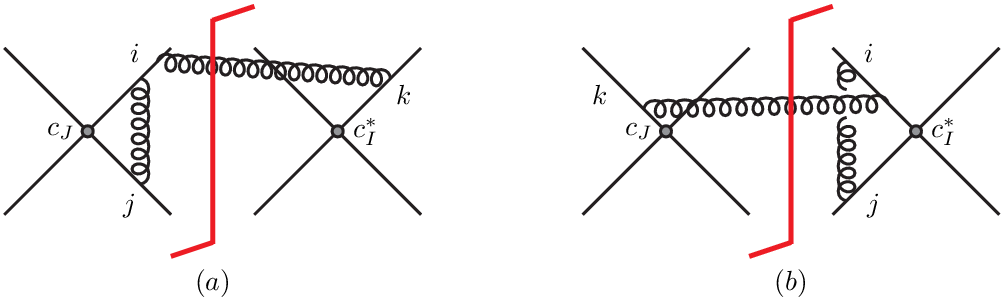
\includegraphics[width=0.7\textwidth]{plots/diagram4-pecjak.png}
  \end{center}
  \caption{
    Three-Wilson-line, mixed real-virtual integrals, which add up to scaleless
    integral.
  }
  \label{fig:pecjak4}
\end{figure}
%

The single-gluon cut integrals of Fig.~\ref{fig:pecjak4} read
%
\begin{eqnarray}
  \bar{I}_{8, ijk}^{(a)} &= &
  n_i \cdot n_j\; n_i \cdot n_k\; 
  \int d^d k\, d^d l\; 
  \frac{\delta_+(k^2) \,
    \; \delta^{(2)}(q_\perp-k_\perp)}
    {(n \cdot k)^\alpha\; (n \cdot l)^\beta \; 
    n_i \cdot k \; n_i \cdot (k+l) \; n_j \cdot l \; n_k \cdot k} \,,
  \\
  \bar{I}_{8, ijk}^{(b)} &= &
  n_i \cdot n_j\; n_i \cdot n_k\; 
  \int d^d k\, d^d l\; 
  \frac{\delta_+(k^2) \,
    \; \delta^{(2)}(q_\perp-k_\perp)}
    {(n \cdot k)^\alpha\; (n \cdot l)^\beta \; 
    n_i \cdot l \; n_i \cdot (k+l) \; n_j \cdot l \; n_k \cdot k} \,.
  %\label{eq:}
\end{eqnarray}
%
This type of diagrams are scaleless and vanish in the fully massless case
discussed in~\cite{Ferroglia:2012uy} but they do not need to vanish here as in
our case two outgoing legs are massive. 


%-----------------------------------------------------------------------------
\newpage
\section{Boundary terms}

We would like to perform sector decomposition of the following integral
of the prototype PR43
%
\begin{equation}
  I = 
  \int \frac{d^d k\, d^d l\, \delta(k^2) \delta(l^2)\,
             \delta(|k_\perp+l_\perp|^2-1)}
  {(n\cdot k)^{\alpha+1} (n\cdot l)^\alpha (v_3 \cdot l) (k\cdot l)}\,,
  %\label{eq:}
\end{equation}
%
taken at the boundary, which corresponds to $\beta=1$ (or, equivalently $x=1$).

The boundary integral can be parameterized with $k_+$, $k_-$, $l_+$, $l_-$,
$k_T$, $l_T$ and $\phi$, where the latter is the angle between transverse
components of gluons four-momenta. The integration measures in the transverse
plane read
%
\begin{eqnarray}
  d^{d-2} k_\perp & = & 
  \Omega_{1-2\epsilon}\,
  k_T^{1-2\epsilon} \sin^{-2\epsilon}\! \phi\, d k_T\, d\phi\,,
  \\
  d^{d-2} l_\perp & = & 
  \Omega_{2-2\epsilon}\,
  l_T^{1-2\epsilon} d l_T\,.
  %\label{eq:}
\end{eqnarray}
%
\smallcomment{Possible issue with factor 1/2 related to $[0,2\pi]$ range of
$\phi$.}\\
%
It is convenient to replace the angular variable $\phi$ by
%
\begin{equation}
  \eta = \frac{1-\cos\phi}{2}\,.
  %\label{eq:}
\end{equation}
%
Then, the whole measure takes the form
%
\begin{equation}
  d^d k\, d^d l =
  4^{-\epsilon}
  \Omega_{1-2\epsilon}\,
  \Omega_{2-2\epsilon}\;
  k_T^{1-2\epsilon} \,
  l_T^{1-2\epsilon} 
  \big((1-\eta)\eta \big)^{-\frac12-\epsilon}
  dk_+ dk_- dl_+ dl_-
  d k_T\, 
  d l_T\,
  d\eta\,.
  %\label{eq:}
\end{equation}
%
After performing integrations over $k_-$, $l_-$ and $\eta$, we are left with
the following form of the boundary integral
%
\begin{equation}
  I =
  \Sigma
  \int dk_+ dl_+ dk_T dl_T
  \frac{k_+^{-1-\alpha}\, l_+^{1-\alpha} k_T l_T \,
  \Big\{\big[1-(k_T-l_T)^2\big]\big[1-(k_T+l_T)^2\big]
  \Big\}^{-\frac12-\epsilon}
  }{(l_+^2+l_T^2)
  \big(k_T^2 k_+ l_+ +l_T^2 k_+ l_+ + k_T^2 l_+^2 + l_T^2 k_+^2 - k_+ l_+
  \big)
  }\,,
  %\label{eq:}
\end{equation}
%
where $\Sigma$ contains all the constants and the $\delta$ functions generated
the following relations
%
\begin{equation}
  k_- = \frac{k_T^2}{k_+}\,, \qquad \qquad
  l_- = \frac{l_T^2}{l_+},
  %\label{eq:}
\end{equation}
%
and
\begin{equation}
  | k_T - l_T | \leq 1\,,
  \qquad \land \qquad
   k_T + l_T  \geq 1\,.
  \label{eq:kTlT-region}
\end{equation}
%
The last pair of relations defines the integration region in the $(k_T, l_T)$
plane.  This region is depicted in Fig.~\ref{fig:trans-regions}~(left).  The
first inequality in (\ref{eq:kTlT-region}) corresponds to the two solid (red)
lines, while the second inequality corresponds to the dotted (blue) line.

\begin{figure}[t]
  \begin{center}
    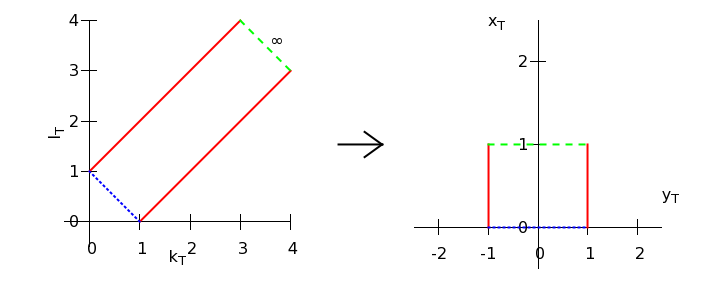
\includegraphics[width=0.99\textwidth]{plots/transverse-phase-space.png}
  \end{center}
  \caption{
  Change of integration region after transformation of transverse coordinates.
  }
  \label{fig:trans-regions}
\end{figure}

The integral $I$ is divergent in the following cases:
%
\begin{enumerate}
  \item
    $k_+ \to 0$, 
    rapidity divergence for gluon $g(k)$
  \item 
    $k_+ \to 0,\ l_+ \to 0$, ???
  \item
    $l_+ \to 0,\ l_T \to 0$, 
    soft divergence for gluon $g(l)$
  \item
    $k_T \to \displaystyle \frac{k_+ }{k_+ + l_+},
    \ l_T \to \frac{l_+ }{k_+ + l_+}$,
    collinear divergence of 3-gluon vertex
\end{enumerate}
%
Let us call the cases 3. and 4. the ``mixed divergences''.

We would like to transform the integration region in the $(\kp, \lp, k_T, l_T)$
space into a hyper-cube and, if necessary, split it such that each of resulting
integrals $\int \prod_i d x_i f(\{x_i\})$ has singularities only in the limits
$x_i \to 0$.
%
We achieve the above in the following steps:
 
%------------------------------------
\subsubsection*{Step 1}

The transverse variables $(k_T, l_T)$ are transformed to new variables 
$(x_T, y_T)$ with the following replacements
%
\begin{equation}
  k_T = \frac{1+y_T-x_T y_T}{2(1-x_T)}\,,
  \qquad \qquad
  l_T = \frac{1-y_T+x_T y_T}{2(1-x_T)}\,,
  %\label{eq:}
\end{equation}
%
and the inverse transformation reads
\begin{equation}
  x_T = 1-\frac{1}{k_T+l_T}\,,
  \qquad \qquad
  y_T = k_T-l_T\,.
  %\label{eq:}
\end{equation}

This results in change of the integration region from the one shown in
Fig.~\ref{fig:trans-regions}~(left) to that of
Fig.~\ref{fig:trans-regions}~(right). The latter corresponds to
%
\begin{equation}
  0 \leq x_T \leq 1
  \qquad \land \qquad
  -1 \leq y_T \leq 1\,.
  %\label{eq:}
\end{equation}

The mixed divergences  now happen at
%
\begin{enumerate}
  \setcounter{enumi}{2}
  \item
    $l_+ \to 0,\ x_T \to 0,\ y_T \to 1$,
  \item
    $x_T \to 0,\ y_T \to \displaystyle \frac{\kp-\lp}{\kp+\lp}$\,.
\end{enumerate}
%
The last divergence occurs on a manifold inside the integration region. This
manifold is depicted in Fig.~\ref{fig:yTmanifold}.

\begin{figure}[t]
  \begin{center}
    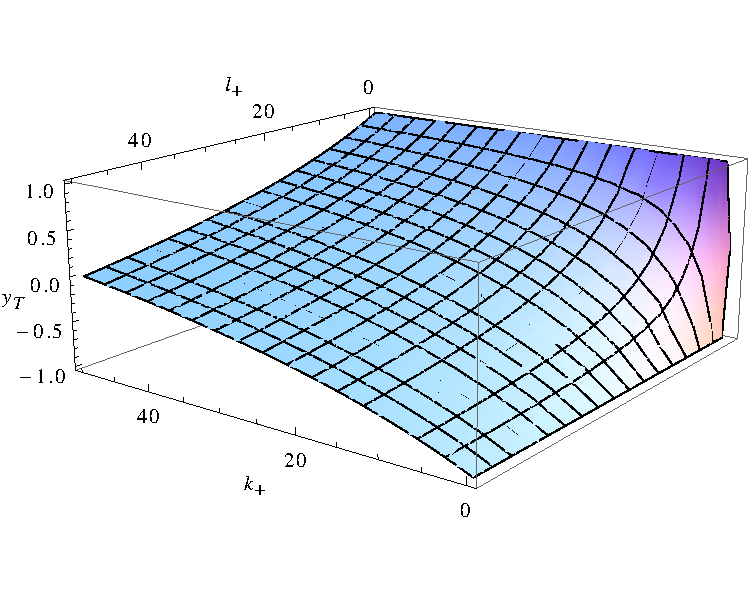
\includegraphics[width=0.49\textwidth]{plots/yTmanifold.pdf}
  \end{center}
  \caption{
  Manifold where the boundary integral becomes singular.
  }
  \label{fig:yTmanifold}
\end{figure}

%------------------------------------
\subsubsection*{Step 2}

In order to transform the manifold singularity into endpoint singularity, we
split the integration region in variable $y_T$ precisely on the manifold of
Fig.~\ref{fig:yTmanifold}
%
\begin{eqnarray}
  I & =  & 
  \int_0^\infty\!\!\! d\kp
  \int_0^\infty\!\!\! d\lp
  \int_0^1\!\!\! d x_T
  \int_{-1}^1\!\!\! d y_T\
  \tilde I(\kp, \lp, x_T, y_T)
  \nonumber \\
  & = &
  \int  d\kp d\lp d x_T
  \int_{-1}^{c(\kp, \lp)}\!\!\! d y_T\
  \tilde I(\kp, \lp, x_T, y_T)
  +
  \int  d\kp d\lp d x_T
  \int_{c(\kp, \lp)}^{1}\!\!\! d y_T\
  \tilde I(\kp, \lp, x_T, y_T)
  \nonumber \\
  & \equiv &
  I_d + I_u\,,
  %\label{eq:}
\end{eqnarray}
%
where
%
\begin{equation}
  c(\kp, \lp) = \frac{\kp-\lp}{\kp+\lp}\,.
  %\label{eq:}
\end{equation}

Now, we use two different parametrizations
%
\begin{equation}
  y_T = \frac{\kp-\lp + 2 \lp \bar y_T}{\kp+\lp}\,,
  \qquad \qquad
  \bar y_T = \frac{y_T-c(\kp,\lp)}{1-c(\kp,\lp)},
  \qquad 
  \text{for}\quad I_u\,,
  %\label{eq:}
\end{equation}
%
and
%
\begin{equation}
  y_T = \frac{\kp-\lp - 2 \lp \bar y_T}{\kp+\lp}\,,
  \qquad
  \bar y_T = \frac{y_T-c(\kp,\lp)}{-1-c(\kp,\lp)},
  \qquad \qquad
  \text{for}\quad I_d\,.
  %\label{eq:}
\end{equation}
%
Hence, we obtain
%
\begin{eqnarray}
 I_d  & =  &
  \int_0^\infty\!\!\! d\kp
  \int_0^\infty\!\!\! d\lp
  \int_0^1\!\!\! d x_T
  \int_{0}^1\!\!\! d \bar y_T\
  \tilde I_1(\kp, \lp, x_T, \bar y_T)\,,
  \\
 I_u  & =  &
  \int_0^\infty\!\!\! d\kp
  \int_0^\infty\!\!\! d\lp
  \int_0^1\!\!\! d x_T
  \int_{0}^1\!\!\! d \bar y_T\
  \tilde I_2(\kp, \lp, x_T, \bar y_T)\,.
  %\label{eq:}
\end{eqnarray}

With the above changes, the mixed singularities happen at
%
\begin{enumerate}
  \setcounter{enumi}{2}
  \item
    $l_+ \to 0,\ x_T \to 0,\ \bar y_T \to 1$,
  \item
    $x_T \to 0,\ \bar y_T \to 0$
\end{enumerate}
%
for $I_u$ and
%
\begin{enumerate}
  \setcounter{enumi}{2}
  \item
    $x_T \to 0,\ \bar y_T \to 0$
\end{enumerate}
%
for $I_d$ and.
%
We see that, in the case of $I_u$, the integral can be divergent at both ends of
$\bar y_T$.

%------------------------------------
\subsubsection*{Step 3}

In order to move all singularities to the limit $x_i \to 0$, we split $I_u$ at 
$\bar y_T = \frac12$
%
\begin{equation}
 I_u = \int_0^1 d \bar y_T\, \tilde I =
 \int_0^\frac12 d \bar y_T\, \tilde I +
 \int_\frac12^1 d \bar y_T\, \tilde I \equiv I_{u0} + I_{u1}\,.
  %\label{eq:}
\end{equation}
%
Then, we apply the following transformations
%
\begin{equation}
  \tilde y_T = 2(1-\bar y_T)\,,
  \qquad \qquad
  \bar y_T = 1-\frac{\tilde y_T}{2}\,,
  \qquad 
  \text{for}\quad I_{u1}\,,
  %\label{eq:}
\end{equation}
%
and
%
\begin{equation}
  \tilde y_T = 2 \bar y_T\,,
  \qquad \qquad
  \bar y_T = \frac{\tilde y_T}{2}\,,
  \qquad 
  \text{for}\quad I_{u0}\,.
  %\label{eq:}
\end{equation}
%
At this point, we have the following mixed singularities:

\begin{displaymath}
  \begin{array}{ll}
   \text{for }  I_{u1}: &
   l_+ \to 0,\ x_T \to 0,\ y_T \to 0,
   \\
    \text{for } I_{u0} \text{ and } I_d: &
    x_T \to 0,\  y_T \to 0\,,
    \\[0.5em]
  \end{array}
\end{displaymath}
 
\noindent
where we dropped tildes and bars for simplicity of notation.

%------------------------------------
\subsubsection*{Step 4}

In the last step, we compress the ranges of the $\kp$ and $\lp$ integrals by the
transformation
%
\begin{equation}
  \kp = \frac{x}{1-x}\,, 
  \qquad \qquad
  \lp = \frac{y}{1-y}\,, 
\end{equation}
%
whose inverse reads
\begin{equation}
  x = \frac{\kp}{1+\kp}\,, 
  \qquad \qquad
  y = \frac{\lp}{1+\lp}\,.
\end{equation}

Hence, finally, our boundary integral is a sum of three contributions
%
\begin{equation}
  I = I_d + I_{u0} + I_{u1}\,,
  %\label{eq:}
\end{equation}
%
which are singular in the following limits: \vspace{10pt}

\noindent
$I_d$:
%
\begin{enumerate}
  \item
  $x \to 0$\,,
  \vspace{-5pt}
  \item
  $x \to 0,\ y \to 0$\,,
  \vspace{-5pt}
  \item
   $ x_T \to 0,\  y_T \to 0$\,,
\end{enumerate}

\noindent
$I_{u0}$:
%
\begin{enumerate}
  \item
  $x \to 0$\,,
  \vspace{-5pt}
  \item
  $x \to 0,\ y \to 0$\,,
  \vspace{-5pt}
  \item
   $ x_T \to 0,\  y_T \to 0$\,,
\end{enumerate}

\noindent
$I_{u1}$:
%
\begin{enumerate}
  \item
  $x \to 0$\,,
  \vspace{-5pt}
  \item
  $x \to 0,\ y \to 0$\,,
  \vspace{-5pt}
  \item
   $y \to 0,\ x_T \to 0,\ y_T \to 0$\,.
\end{enumerate}

%-----------------------------------------------------------------------------
\section{Symmetries between integrals}

Our double-cut, soft function integrals have the general structure
%
\begin{align}
I(\{p_i\}) &= \int d^dk\, d^d l\, \delta^{(+)}(k^2) \delta^{(+)}(l^2)
     h(p_i\cdot p_j, p_i\cdot k, p_i \cdot l)\,
     \delta(1-|k_\perp+l_\perp|)\,.
\end{align}
%
Because of the transverse delta function, these integrals are invariant
only under a subgroup of the Lorentz group which involves:
%
\begin{itemize}
  %\setlength\itemsep{1.2em}
  \item
  rescaling of the light-cone components of the momenta $k$ and $l$ compensated
  by inverse rescaling of the light-cone components of the external momenta,
  \item
  rotations of the above momenta in the transverse plane.
\end{itemize}
%
Let us denote
\begin{align}
  p\cdot q & \quad \text{usual, $d$-dimensional scalar product}\,, \\
  p * q & = p_0 q_0 - p_3 q_3 = p_+ q_- + p_- q_+\,.
\end{align}


\begin{enumerate}
  \item
  Given the above, reduced Lorentz symmetry, and the fact that the result can
  only depend on external momenta, we conclude, that our integral must be a
  function of $p_i * p_j$ and $p_{i,\perp} \cdot p_{j,\perp}$ or, equivalently,
  $p_i * p_j$ and $p_i \cdot p_j$.

  \item
  The integrand is invariant under the rescaling of $p_3 = \lambda_3 p_3$
  and $p_4 = \lambda_4 p_4$, which means that the result can only be a function
  of ratios of the above scalar products.

  \item
  Integrals which do not exhibit $\alpha$ poles are also invariant under
  rescaling of $p_1$. But, here, one cannot form a variable of the type $p_1
  \cdot p_3/\sqrt{p_1^2 p_3^2}$ because $p_1$ is massless. As a consequence, the
  only possibility is $p_3^{*2}/p_3^2 = p_4^{*2}/p_4^2 $. This is why some
  abelian integrals $13$ and $14$ are equal.

  \item
  In case with $\alpha$ poles, rescaling of $p_1$ is broken 
  %
  \begin{displaymath}
    I(\lambda p_1) =  \lambda^{-\alpha} I(p_1)\,,
  \end{displaymath}
  %
  but its form can be
  deduced from  the integrand. For example, for the case of graphs involving
  lines 1 and 3, the above means that the only way $p_1$ can enter is through a
  prefactor and 
  %
  \begin{displaymath}
    I(\{p_i\}) =  \left(\frac{p_1\cdot p_3}{\sqrt{p_3^2}}\right)^{-\alpha} 
    I(\{p_i\}\backslash \{p_1\})\,.
  \end{displaymath}
  (Possibly also $\left(p_1\cdot p_3/\sqrt{p_3^{*2}}\right)^{-\alpha}$.)

\end{enumerate}


%-----------------------------------------------------------------------------
\chapter{Renormalization}

%-----------------------------------------------------------------------------
\section{Beam functions from RGE}

We define
%
\begin{equation}
  I_{ij}(z,\Lp) = I^{(0)}(z,\Lp) +
  \asp I^{(1)}_{ij}(z,\Lp) + \left(\asp\right)^2 I^{(2)}_{ij}(z,\Lp) + \ldots\,.
  %\label{eq:}
\end{equation}
%
From RGE we obtain
%
\begin{subequations}
  %\label{eq:}
  \begin{align}
  I^{(0)}_{ij}(z,\Lp) & = 
  \delta_{ij} \delta(1-z)\,,\\
  %
  I^{(1)}_{ij}(z,\Lp) & = 
  \left[\Gamma^{(0)}_i \frac{\Lp^2}{4} - \gamma^{(0)}_i \Lp \right]
  \delta_{ij} \delta(1-z) - P^{(0)}_{ij} (z) \Lp + R^{(0)}_{ij}(z)\,, \\
  \\
  %
  I^{(2)}_{ij}(z,\Lp) & = 
  \left[
  \left(\Gamma^{(0)}_i\right)^2 \frac{\Lp^4}{32}
  -\Gamma^{(0)}_i\left(3\gamma^{(0)}_i 
  - \beta_0 \right) \frac{\Lp^3}{12}
  + \gamma^{(0)}_i\left(\gamma^{(0)}_i - \beta_0 \right)\frac{\Lp^2}{2}
  \right] \delta_{ij} \delta(1-z) 
  \nonumber \\
  & 
  -\Gamma^{(0)}_i P^{(0)}_{ij} \frac{\Lp^3}{6} 
  +\Gamma^{(0)}_i R^{(0)}_{ij} \frac{\Lp^2}{4} 
  +\left(\gamma^{(0)}_i -\beta_0\right) P^{(0)}_{ij} \frac{\Lp^2}{2} 
  -\left(\gamma^{(0)}_i -\beta_0\right) R^{(0)}_{ij} \Lp
  \nonumber \\
  & 
  + \left[
  \Gamma^{(1)}_i \frac{\Lp^2}{4}-\gamma^{(1)}_i \Lp
  \right] \delta_{ij} \delta(1-z)
  - P^{(1)}_{ij}(z)\Lp
  -\left[
  \Gamma^{(0)}_i \frac{\Lp^3}{12}-\gamma^{(0)}_i \frac{\Lp^2}{2}
  \right] P^{(0)}_{ij}(z) 
  \nonumber \\
  &
  + D_{ij}(z)\frac{\Lp^2}{2} - E_{ij}(z) \Lp + R^{(1)}_{ij}(z)\,.
  \end{align}
\end{subequations}
%
The anomaly exponent reads
\begin{equation}
  g_i (\Lp,\as) =  
  - \left(\ln \frac{M^2}{\mu^2} + \Lp\right) F_{i\bar i}(\Lp,\as)\,,
  %\label{eq:}
\end{equation}
%
with
%
\begin{equation}
  F_{i\bar i}(\Lp,\as) = 
  \asp \Gamma^{(0)}_i \Lp + 
  \left(\asp\right)^2 
  \left( \Gamma^{(0)}_i \frac{\beta_0}{2}\Lp^2 +\Gamma^{(1)}_i \Lp + d_{i,2}
  \right)\,.
  %\label{eq:}
\end{equation}
%
With the above, we define
%
\begin{equation}
  C_{i\bar i \gets a b} = 
  e^{g_i (\Lp, \as)}\, I_{ia}(z_1,\Lp, \as)\, I_{\bar i b}(z_2,\Lp, \as) \,
  {\rm HS}_{\iibar}(\Lp, \as)
  %\label{eq:}
\end{equation}


%-----------------------------------------------------------------------------
\subsection{Leading logarithmic coefficient in $qg \to gg$ channel}

The highest term this case is $\Lp^3$. The coefficient in front gets
contributions from three sources
%

\begin{displaymath}
  \begin{array}{ccc}
    I^{(1)}_{gq} I^{(1)}_{gg} & \mapsto & 
    -\frac{1}{4} \Gamma^{(0)}_g \delta(1-z_2) P^{(0)}_{gq}(z_1)\,, \\[1em]
    %
    I^{(2)}_{gq} I^{(0)}_{gg} & \mapsto & 
    -\frac{1}{4} \Gamma^{(0)}_g \delta(1-z_2) P^{(0)}_{gq}(z_1)\,, \\[1em]
    %
    g_g I^{(1)}_{gq}I^{(0)}_{gg}  & \mapsto & 
    \Gamma^{(0)}_g \delta(1-z_2) P^{(0)}_{gq}(z_1)\,.
    %
  \end{array}
\end{displaymath}
%
Hence, the overall result reads
\begin{equation}
    C_{gg\gets qg}^\text{LL} = 
    \frac12 \Gamma^{(0)}_g\, \delta(1-z_2)\, P^{(0)}_{gq}(z_1)\, \Lp^3\,,
  %\label{eq:}
\end{equation}
%
which, after Fourier transform corresponding to the
replacement~\cite{Li:2013mia}
%
\begin{equation}
  \Lp^3 \to -\left[\frac{3}{q_T^2} \ln^2\frac{\mu^2}{q_T^2}\right]^{[\mu^2]}_*
  - 4\zeta_3\delta(q_T^2)\,,
  %\label{eq:}
\end{equation}
%
for $q_T>0$, where we keep only the first term in which we can ignore the
'*' prescription, gives
%
\begin{equation}
    C_{gg\gets qg}^\text{LL} = 
    -\frac{3}{2} \Gamma^{(0)}_g\, \delta(1-z_2)\, P^{(0)}_{gq}(z_1)\,
    \frac{1}{q_T^2} \ln^2\frac{\mu^2}{q_T^2}\,.
  %\label{eq:}
\end{equation}
  



%-----------------------------------------------------------------------------
\newpage
\section{Soft function from RGE}

%-----------------------------------------------------------------------------
\subsection{Introductory considerations}

The renormalized soft function of small-$q_T$ factorization satisfies the
following RGE equation~\cite{Zhu:2012ts}
%
\begin{equation}
  \frac{d}{d\ln \mu} \bfS_\iibar (\mu) =
  - \bfgamma^{s \dagger}_\iibar \,\bfS_\iibar (\mu)  
  - \bfS_\iibar (\mu)\, \bfgamma^{s}_\iibar \,,
  \label{eq:SF-RGE-main}
\end{equation}
%
where
%
\begin{equation}
  \bfgamma^{s}_\iibar = \bfgamma^{h}_\iibar - 2 \gamma^{i} \bfI\,,
  %\label{eq:}
\end{equation}
%
and $\bfgamma^{h}_\iibar$ is defined as a non-$\Gamma_\text{cusp}$ part of the
full anomalous dimension matrix $\bfGamma$~\cite{Ahrens:2010zv}, while
$\gamma^{i}$ is the massless-particle anomalous dimension (enters RGE
equations for beam functions in Drell-Yan and Higgs
production~\cite{Becher:2010tm, Becher:2012yn}). To make the notation lighter, to
this end, we shall omit the index $\iibar$, keeping in mind that the soft
function and the anomalous dimension are different in the \qqbar and $gg$
channels.

The soft anomalous dimension matrix $\bfgamma^{s}$ is related to the soft
renormalization factor (also a matrix in colour space), $\bfZ_s$, as follows
%
\begin{equation}
  \bfgamma^{s} = - \bfZ_s^{-1}\frac{d\bfZ_s}{d\ln \mu}\,,
  %\label{eq:}
\end{equation}
%
and $\bfZ_s$ absorbs all UV divergences such that~\footnote{
A quick consistency check:
%
\begin{eqnarray}
  \frac{d}{d\ln \mu} \bfS(\mu) 
  = 
  \frac{d\bfZ^\dagger_s}{d\ln\mu} \bfS_\bare \bfZ_s +
  \bfZ^\dagger_s \bfS_\bare \frac{d\bfZ_s}{d\ln\mu}
  =
  \underbrace{\frac{d\bfZ^\dagger_s}{d\ln\mu}
  (\bfZ^{-1}_s)^{^\dagger}}_{-\bfgamma^{s \dagger}}
  \underbrace{\bfZ^\dagger_s \bfS_\bare \bfZ_s}_{\bfS(\mu)}
  +
  \underbrace{\bfZ^\dagger_s \bfS_\bare \bfZ_s}_{\bfS(\mu)}
  \underbrace{\bfZ_s^{-1} \frac{d\bfZ_s}{d\ln\mu}} _{-\bfgamma^{s }}\,.
  %\label{eq:}
\end{eqnarray}
}

%
\begin{equation}
  \bfS(\mu) = \bfZ^\dagger_s(\mu,\epsilon) \bfS_\bare(\epsilon)
  \bfZ_s(\mu,\epsilon)\,.
  %\label{eq:}
\end{equation}
%
Each quantity in the above equation has perturbative expansion, either in the
renormalized coupling, $a_s =
\frac{\alpha_s}{4\pi}$, or in the bare coupling,
$a_s^0 = \frac{\alpha_s^0}{4\pi}$, and the relation between the two is
%
\begin{equation}
  a_s^0(\epsilon) = 
  \left(\frac{\mu^2 e^{\gamma_E}}{4\pi}\right)^\epsilon Z_\alpha a_s
  \equiv \xi_\as(\epsilon,\mu)\, Z_\alpha\, a_s (\mu)\,,
\end{equation}
%
where the \msbar renormalization constant reads
%
\begin{equation}
  Z_\alpha = 
  1- \frac{\beta_0 \as}{4\pi \epsilon} + \ldots =
  1- \frac{\beta_0}{\epsilon} a_s(\mu) + \ldots\,.
  \label{eq:Zalpha}
\end{equation}
%
Hence, we can write
%
\begin{eqnarray}
  \bfS(\mu) & = &  
  \bfS^{(0)}(\mu) + a_s(\mu)\, \bfS^{(1)}(\mu) + a_s^2(\mu)\, \bfS^{(2)}(\mu) 
  + \order{a_s^3}
  \nonumber \\
  & = & 
  \left(\bfZ^{\dagger (0)}_s(\epsilon, \mu) + 
  a_s(\mu)\,\bfZ^{\dagger (1)}_s(\epsilon, \mu) + 
  a_s^2(\mu)\,\bfZ^{\dagger (2)}_s(\epsilon, \mu)  \right)
  \nonumber \\ & &
  \times \left(\bfS^{(0)}_\bare(\epsilon) + 
  a_s(\mu)\, \xi_\as(\epsilon, \mu)\, Z_\alpha\, \bfS^{(1)}_\bare(\epsilon) 
  + a_s(\mu)^2\, \xi_\as^2(\epsilon, \mu)\, Z_\alpha^2\,
    \bfS^{(2)}_\bare(\epsilon) \right)
  \\ & &
  \times 
  \left(\bfZ^{(0)}_s(\epsilon, \mu) + a_s(\mu)\,\bfZ^{(1)}_s(\epsilon, \mu) + 
  a_s(\mu)^2\,\bfZ^{(2)}_s(\epsilon, \mu)  \right)\,,
  \nonumber
  %
  %\label{eq:}
\end{eqnarray}
%
and, with Eq.~(\ref{eq:Zalpha}) and $\bfZ_s^{(0)} = \bfI$, we get
%
\begin{eqnarray}
  \bfS(\mu) & = &  
  \bfS^{(0)}(\mu) + a_s(\mu)\, \bfS^{(1)}(\mu) + a_s^2(\mu)\, \bfS^{(2)}(\mu) 
  \nonumber \\
  & = & 
  \left(\bfI + 
  a_s(\mu)\,\bfZ^{\dagger (1)}_s(\epsilon, \mu) + 
  a_s^2(\mu)\,\bfZ^{\dagger (2)}_s(\epsilon, \mu)  \right)
  \nonumber \\ & &
  \times \left(\bfS^{(0)}_\bare(\epsilon) + 
  a_s(\mu)\, \xi_\as \bfS^{(1)}_\bare(\epsilon) -
  a_s(\mu)^2\, \xi_\as\,  \frac{\beta_0}{\epsilon}\, \bfS^{(1)}_\bare(\epsilon) 
  + a_s(\mu)^2\, \xi_\as^2\, 
    \bfS^{(2)}_\bare(\epsilon) \right)
  \nonumber \\ & &
  \times 
  \left(\bfI+ a_s(\mu)\,\bfZ^{(1)}_s(\epsilon, \mu) + 
  a_s(\mu)^2\,\bfZ^{(2)}_s(\epsilon, \mu)  \right)\,,
  \nonumber
  %
  %\label{eq:}
\end{eqnarray}
%
which  gives us the following, order-by-order relations
%
\begin{eqnarray}
  \bfS^{(0)} & = &  \bfS^{(0)}_\bare \,,
  \\[0.5em]
  \bfS^{(1)} & = &
  \bfZ^{\dagger (1)}_s \bfS^{(0)}_\bare  + \bfS^{(0)}_\bare \bfZ^{(1)}_s  +
  \xi_\as \bfS^{(1)}_\bare \,,
  \\[0.5em]
  \bfS^{(2)} & = &
  \bfZ^{\dagger (2)}_s \bfS^{(0)}_\bare  + \bfS^{(0)}_\bare \bfZ^{(2)}_s  +
  \bfZ^{\dagger (1)}_s \bfS^{(0)}_\bare \bfZ^{(1)}_s 
  \nonumber \\[0.5em]
  & &
  + \bfZ^{\dagger (1)}_s \xi_\as \bfS^{(1)}_\bare  + 
  \xi_\as \bfS^{(1)}_\bare \bfZ^{(1)}_s  +
  \xi_\as^2 \bfS^{(2)}_\bare 
  -\frac{\beta_0}{\epsilon}\, \xi_\as \bfS^{(1)}_\bare
  \,.
  \label{eq:S2ren}
\end{eqnarray}
%
The quantities on the l.h.s. are $\epsilon$-independent. The $\bfZ^{(i)}_s$
factors have only singular terms with poles in $\epsilon$, while the bare
functions, $\bfS^{(1)}_\bare$ and $\bfS^{(2)}_\bare$, have both singular and
finite parts.

We can now absorb the $\xi_\as$ prefactors into the definitions of the bare
soft functions and change the notation according to
%
\begin{equation}
  \tbfS^{(n)}_\bare \equiv \xi_\as^n \bfS^{(n)}_\bare\,.
  %\label{eq:}
\end{equation}
%

Specifically, at the order $a_s^2$, from Eq.~(\ref{eq:S2ren}), we get
%
\begin{eqnarray}
  \underbrace{\bfS^{(2)}}_{\text{finite part only}}   
  &  =  &
  \overbrace{\bfZ^{\dagger (2)}_s \tbfS^{(0)}_\bare  + 
   \tbfS^{(0)}_\bare \bfZ^{(2)}_s  +
   \bfZ^{\dagger (1)}_s \tbfS^{(0)}_\bare \bfZ^{(1)}_s}^{\text{(I) pole part only}} 
  \nonumber \\
  & &
  \quad +  \quad 
  \underbrace{\bfZ^{\dagger (1)}_s \tbfS^{(1)}_\bare  + 
  \tbfS^{(1)}_\bare \bfZ^{(1)}_s  +
  \tbfS^{(2)}_\bare
 -\frac{\beta_0}{\epsilon}\, \tbfS^{(1)}_\bare
  }_{\text{(II) finite + pole part}} \,.
  \label{eq:renS2}
\end{eqnarray}
%
The  part (I) on the r.h.s. has only terms singular in $\epsilon$, which come
from the fact that the $\bfZ_s$ factors are defined in the \msbar scheme. 

These pole terms have to cancel against singular terms of part (II). And that
can be used in the following way:
%
Knowing $\bfZ_s^{(1)}$ and $\bfZ_s^{(2)}$, as well as $\tbfS^{(0)}_\bare$ and
$\tbfS^{(1)}_\bare$, allows one to cross-check all the singular terms of
the $\tbfS^{(2)}_\bare$ function obtained from direct calculation.

To this end, for notational simplicity, we abandon tilde in the soft function
symbol and assume that the latter always includes the appropriate power of
$\xi_\as$.

%Assuming that all the pole terms cancel, as they should, we have
%%
%\begin{equation}
%  \bfS^{(2)} = 
%  \left[\bfZ^{\dagger (1)}_s \bfS^{(1)}_\bare\right]_{\text{finite part}}  + 
%  \left[\bfS^{(1)}_\bare \bfZ^{(1)}_s\right]_{\text{finite part}}  +
%  \left[\bfS^{(2)}_\bare\right]_{\text{finite part}}\,,
%\end{equation}
%% 
%and we can use the already known results for
%$\bfS^{(1)}_\bare$ and  $\bfZ^{(1)}_s$ to determine the RG-induced part of
%$\bfS^{(2)}$. For that we do not even need to know $\bfZ^{(2)}_s$.


%%
%\begin{eqnarray}
%  \overbrace{\bfS^{(2)}}^{\text{finite part only}}  & =  &
%  \overbrace{\bfZ^{\dagger (2)}_s \bfS^{(0)}_\bare  + \bfS^{(0)}_\bare \bfZ^{(2)}_s  +
%  \bfZ^{\dagger (1)}_s \bfS^{(0)}_\bare \bfZ^{(1)}_s}^{\text{pole part only}} 
%  %\nonumber \\
%  %& &
%  %+ \
%  \underbrace{\bfZ^{\dagger (1)}_s \bfS^{(1)}_\bare  + \bfS^{(1)}_\bare \bfZ^{(1)}_s  +
%  \bfS^{(2)}_\bare}_{\text{finite + pole part}} \,.
%  %\label{eq:}
%\end{eqnarray}

%-----------------------------------------------------------------------------
\subsection{Determination of $\mathbold{L_\perp^n}$-dependent terms of the soft
function}
\label{sec:RGevolution}


The RGE evolution equation (\ref{eq:SF-RGE-main}) can be written as
%
\begin{equation}
  \frac{d}{d L_\perp} \bfS(\mu) =
  - \frac{1}{2} \left[
  \bfgamma^{s \dagger}\,\bfS(\mu)  
  + \bfS(\mu)\, \bfgamma^{s}
  \right]\,,
  \label{eq:SF-RGE-Lp}
\end{equation}
%
where
%
\begin{equation}
  L_\perp = \ln\frac{\mu^2 x_T^2}{b_0^2}
  \qquad \qquad
  \text{and}
  \qquad \qquad
  b_0 =  2 e^{- \gamma_E}\,.
  %\label{eq:}
\end{equation}
%
Both the soft function and the anomalous dimension have perturbative expansions
%
\begin{eqnarray}
  \bfS  & = &
  \bfS^{(0)} + a_s \bfS^{(1)} + a_s^2 \bfS^{(2)} + \ldots\,,
  \label{eq:Sren-exp}
  \\
  \bfgamma_{s} & = &
  a_s \left(\bfgamma_{s,0} + a_s \bfgamma_{s,1}+ \ldots\right)\,.
  \label{eq:gammas-exp}
\end{eqnarray}
%
All quantities in the above equations are renormalized and in 4 dimensions.
 
Because the anomalous dimension matrix starts at the order $a_s$,
Eq.~(\ref{eq:SF-RGE-Lp}) can be solved iteratively. We just need to plug
Eqs.~(\ref{eq:Sren-exp}) and (\ref{eq:gammas-exp}) into 
Eq.~(\ref{eq:SF-RGE-Lp}) and  remember that the renormalized, 4-dimensional
coupling $a_s$ also depends on $\ln\mu$, which implies
%
\begin{equation}
  \frac{d a_s}{dL_\perp} = \frac12 \frac{d a_s}{d\ln\mu} = 
  \frac12 \frac{\partial a_s}{\partial \ln\mu} = 
  \frac12 \frac{\beta(a_s)}{4\pi} = 
  - \beta_0\, a_s^2 + \order{a_s^3}\,.
  %\label{eq:}
\end{equation}

After collecting terms at each order, we
arrive at the following differential equations
%
\begin{eqnarray}
  \frac{d}{dL_\perp} \bfS^{(0)} & = &  0\,,
  \\
  \frac{d}{dL_\perp} \bfS^{(1)} & = & 
  -\frac12\left[
  \bfS^{(0)}\, \bfgamma_{s,0} + \bfgamma_{s,0}^\dagger\, \bfS^{(0)} 
  \right]\,,
  \\
  \frac{d}{dL_\perp} \bfS^{(2)} & = & 
  -\frac12\left[
  \bfS^{(1)}\, \bfgamma_{s,0} + \bfgamma_{s,0}^\dagger\, \bfS^{(1)}  
  - 2 \beta_0 \bfS^{(1)}  +
  \bfS^{(0)}\, \bfgamma_{s,1} + \bfgamma_{s,1}^\dagger\, \bfS^{(0)} 
  \right]\,.
  %\label{eq:}
\end{eqnarray}
 
Hence, knowing the soft anomalous dimension to the order $a_s^2$, and the soft
function to the order~$a_s^1$ allows one to determine all pieces of the soft
function at the order $a_s^2$ except the constant term. Specifically, we get
%
\begin{eqnarray}
  \bfS^{(2)} 
  & = & 
  -\frac12\Bigg\{
  \frac12\left[
  \bfS^{(1)}_{L_\perp}\, \bfgamma_{s,0} + 
  \bfgamma_{s,0}^\dagger\, \bfS^{(1)}_{L_\perp}  
  - 2 \beta_0 \bfS^{(1)}_{L_\perp}  +
  \bfS^{(0)}\, \bfgamma_{s,1} + \bfgamma_{s,1}^\dagger\, \bfS^{(0)} 
  \right] L_\perp^2
   \\
  & &
  \hspace{25pt} + \left[
  \bfS^{(1)}_\text{const}\, \bfgamma_{s,0} + 
  \bfgamma_{s,0}^\dagger\, \bfS^{(1)}_\text{const}  
  - 2 \beta_0 \bfS^{(1)}_\text{const}  +
  \bfS^{(0)}\, \bfgamma_{s,1} + \bfgamma_{s,1}^\dagger\, \bfS^{(0)} 
  \right] L_\perp
  \Bigg\} 
  + \text{const}\,,
  \nonumber
  %\nonumber \\
  %& &
  %+ \text{const}.
  %\label{eq:}
\end{eqnarray}
%
where $\bfS^{(1)}_{L_\perp}$ and $\bfS^{(1)}_\text{const}$ denote, respectively,
the $L_\perp$-dependent and $L_\perp$-independent pieces of the $\bfS^{(1)}$
soft function.

%-----------------------------------------------------------------------------
\section{HS functions}

The soft and the hard functions enter the cross section through the trace of
their product
%
\begin{equation}
  \text{Tr} \left[\mathbold{H}_{\iibar}(M, m_t, \cos\theta, \mu) 
                  \mathbold{S}_{\iibar}(M, m_t, \cos\theta, \LT)\right] = 
  \frac{3\as^2}{8 d_i} \sum_{n=0}  \sum^{n}_{m=0}
  \left(\asp\right)^n \LT^m\,
  \text{HS}^{(n,m)}_\iibar\,.
  %\label{eq:}
\end{equation}
%
The only source of $\LT$ is the soft function. Hence, we have the following
contributions
%
\begin{align}
  \text{HS}^{(0,0)} & 
  \quad \leftarrow  \quad \mathbold{H}^{(0)} \mathbold{S}^{(0,0)}\,, \\
  \text{HS}^{(1,1)} & 
  \quad \leftarrow  \quad \mathbold{H}^{(0)} \mathbold{S}^{(1,1)}\,, \\
  \text{HS}^{(1,0)} & 
  \quad \leftarrow  \quad \mathbold{H}^{(0)} \mathbold{S}^{(1,0)},\ 
	                  \mathbold{H}^{(1)} \mathbold{S}^{(0,0)}\,, \\
  \text{HS}^{(2,2)} & 
  \quad \leftarrow  \quad \mathbold{H}^{(0)} \mathbold{S}^{(2,2)}\,, \\
  \text{HS}^{(2,1)} & 
  \quad \leftarrow  \quad \mathbold{H}^{(0)} \mathbold{S}^{(2,1)},\ 
	                  \mathbold{H}^{(1)} \mathbold{S}^{(1,1)}\,.
\end{align}


%-----------------------------------------------------------------------------
\section{Anomalous dimension}

A velocity-dependent part of the anomalous dimension can be written in a compact
form as~\cite{Ferroglia:2009ii, Kidonakis:2009ev}
%
\begin{eqnarray}
   \label{eq:vel-dep-ad}
   \gamma_{\rm cusp}(\beta,\alpha_s)
   &=& \gamma_{\rm cusp}(\alpha_s)\,\beta\coth\beta \nonumber\\
   &&\hspace{-22mm}\mbox{}+ \frac{C_A}{2} 
    \left( \frac{\alpha_s}{\pi} \right)^2 
    \Bigg\{ \frac{\pi^2}{6} + \zeta_3 + \beta^2 
    + \coth^2\beta \left[ \mbox{Li}_3(e^{-2\beta}) 
    + \beta\,\mbox{Li}_2(e^{-2\beta}) - \zeta_3 
    + \frac{\pi^2}{6}\,\beta + \frac{\beta^3}{3} \right] \\
   &&\quad\mbox{}+ \coth\beta \left[ 
    \mbox{Li}_2(e^{-2\beta}) - 2\beta\,\ln(1-e^{-2\beta}) 
    - \frac{\pi^2}{6}\,(1+\beta) - \beta^2 - \frac{\beta^3}{3} 
    \right] \Bigg\}
    + {\cal O}(\alpha_s^3) \,, \nonumber
\end{eqnarray}
%
where $\beta$ is a cusp angle discussed below.


%------------------------------------
\subsection{Cusp angles}

The amplitudes are functions of \emph{Lorentz invariants}~\cite{Becher:2009kw}
%
\begin{equation}
  s_{ij} \equiv 2 \sigma_{ij} p_i \cdot p_j + \iep\,,
  \label{eq:sij-def}
\end{equation}
%
and
\begin{equation}
  p_i^2 = m_i^2\,,
  %\label{eq:}
\end{equation}
%
where
%
\begin{eqnarray}
  \sigma_{ij} = \left\{
    \begin{array}{cl} 
      + 1 &  \text{if } p_i, p_j \text{ are both incoming or outgoing} \\
      - 1 &  \text{otherwise}
    \end{array}
    \right.\,.
  %\label{eq:}
\end{eqnarray}
%
For massive particles we define \emph{four-velocities}
%
\begin{equation}
  v_i \equiv  \frac{p_i}{m_i}\,,
  \qquad \qquad v_i^2 = 1\,.
  %\label{eq:}
\end{equation}
%
We also define \emph{abbreviations}
%
\begin{equation}
  w_{ij} \equiv - \sigma_{ij} v_i \cdot v_j - \iep\,.
  %\label{eq:}
\end{equation}
%
We label massless particles with lowercase $i, j, \ldots$ and massive
ones with capital indices $I, J, \ldots$.

The soft anomalous dimension is a function of \emph{cusp angles}, $\beta_{ij}$, 
$\beta_{Ij}$ and $\beta_{IJ}$, formed by massless and/or massive Wilson lines. They
read~\cite{Becher:2009kw}
%
\begin{subequations}
  %\label{eq:}
  \begin{align}
    \beta_{ij} & = 
    \ln \frac{-2 \sigma_{ij}\, p_i \cdot p_j\, \mu^2}{(-p_i^2)(-p_j^2)} =
    L_i + L_j - \ln\frac{\mu^2}{-s_{ij}}\,,
    \\
    \beta_{Ij} & = 
    \ln \frac{-2 \sigma_{ij}\, v_I \cdot p_j\, \mu}{(-p_j^2)} =
    L_j - \ln\frac{m_I \mu}{-s_{ij}}\,,
    \\
   \label{eq:betaIJ-def}
    \beta_{IJ} & =  {\rm arccosh} \left(w_{IJ}\right) = 
                    {\rm arccosh} \left(\frac{-s_{IJ}}{2 m_I m_J}\right)\,,
  \end{align}
\end{subequations}
%
where we have introduced
%
\begin{equation}
  L_i = \ln \frac{\mu^2}{(-p_i^2)}\,,
  %\label{eq:}
\end{equation}
%
which comes from regularization of IR divergences in effective theory by taking
massless partons slightly off-shell $(-p_i^2) > 0$~\cite{Becher:2009qa}. The
logarithms $L_i$ need to cancel in the final result for the anomalous dimension
matrix.


%------------------------------------
\subsubsection{$\mathbold{\betaIJ}$ in space-like kinematics}

For space-like kinematics of heavy particles (\eg a top quark incoming
and a top quark outgoing), the cusp angle $\beta_{IJ}$ is real. It
can still, however, be chosen to be positive or negative, as the function $\text{arccosh}$
has two branches, even for real argument. 
%
If we look at the first term in Eq.~(\ref{eq:vel-dep-ad}), we notice that it will
be positive regardless of the sign of $\beta_{IJ}$ because $\coth(\beta_{IJ}) >
0$ for $\betaIJ > 0$ and $\coth(\beta_{IJ}) < 0$ for $\betaIJ < 0$.
 
The choice of positive $\betaIJ$ has, however, at least two advantages: (i)
functions that appear in the $\order{\as^2}$ contribution in
Eq.~(\ref{eq:vel-dep-ad}) are real (in the space-like case) and do not require
analytic continuation, as $0 < x < 1$ for $\Li_{2,3}(x)$ and for $\ln(x)$, (ii),
$\coth(\betaIJ)$ has a physical interpretation as an inverse of a relative
velocity between particles $I$ and $J$, $\vIJ$, which reads
%
\begin{equation}
  \coth(\betaIJ) = \frac{1}{\vIJ}\,,
  \label{eq:cothbetaIJ}
\end{equation}
%
where
%
\begin{equation}
  v_{IJ} = \sqrt{1- \frac{4 m_t^4}{s_{IJ}^2}}\,.
  %\label{eq:}
\end{equation}
%
One can show that taking $\betaIJ < 0$ in Eq.~(\ref{eq:vel-dep-ad}), applying
polylogarithm identities and analytic continuation of the logarithm, leaves the
function in Eq.~(\ref{eq:vel-dep-ad}) unchanged~\cite{AnalyticContinuation}.

The choice $\betaIJ>0$ implies $\vIJ > 0$ and this leads to the following
relation between the latter and the $\beta$ function introduced in
Eq.~(\ref{eq:beta-def})~\cite{MyNotes}
%
\begin{equation}
  \vIJ = \frac{2 \beta}{1+\beta^2}\,.
  \label{eq:vIJ-beta-rel}
\end{equation}
%
We notice that~\cite{MyNotes}
%
\begin{equation}
  \beta = \sqrt{\frac{s-1}{s+1}}\,, \qquad \text{where} \qquad 
  s = \frac{\sIJ}{2 m_t^2}\,,
  %\label{eq:}
\end{equation}
%
which means that
%
\begin{equation}
  \begin{array}{lll}
    \text{space-like:}\quad & s < -1 \quad & \beta \in [1,\infty]\,, \\[0.5em]
    \text{time-like:}\quad & s > 1 \quad & \beta \in [0,1]\,.
  \end{array}
  %\label{eq:}
\end{equation}
%
We also note that $\vIJ \in [0,1]$ both in the space-like and in the time-like
case.


Eq.~(\ref{eq:cothbetaIJ}) has a unique solution for the space-like case with
$\betaIJ >0$~\cite{MyNotes}
%
\begin{equation}
  \betaIJ =  -\frac12 \ln \frac{1-\vIJ}{1+\vIJ}\,,
  \label{eq:betaIJ-vIJ}
\end{equation}
%
which, with help of Eq.~(\ref{eq:vIJ-beta-rel}) can be expressed as
%
\begin{equation}
 \betaIJ = -\frac12 \ln\left[\left(\frac{\beta-1}{\beta+1}\right)^2\right]
         = \ln\left[\frac{\beta+1}{\beta-1}\right]\,,
  \qquad \beta \in [1,\infty].
  \label{eq:betaIJ-beta}
\end{equation}

%------------------------------------
\subsubsection{$\mathbold{\betaIJ}$ in time-like kinematics}

We would like to analytically continue $\betaIJ$ to the time-like region which
corresponds to $\sIJ > 0$. The function in Eq.~(\ref{eq:betaIJ-beta}) has a cut
at imaginary axis and, depending whether we cross it in the upper or the
lower half-plane, we get a different result.

The convention is already established in Eqs.~(\ref{eq:sij-def}).
It implies that the invariant $\sIJ$  has a small
positive part which corresponds to analytic continuation over the upper
half-plane. And this means that $\betaIJ$ acquires imaginary part $- i \pi$ in
the time-like region~\cite{AnalyticContinuation}. The real part is identical to
the one of space-like kinematics and at the end we get
%
\begin{equation}
  \betaIJ = \ln\left(\frac{1+\beta}{1-\beta}\right) - i \pi\,,
  \qquad \beta \in [0,1]\,.
  %\label{eq:}
\end{equation}


%%------------------------------------
%\subsection*{Cusp angle of a $\mathbold{t\bar t}$ pair}
%
%Let us now calculate the cusp angle between \ttbar quarks, $\beta_{34}$. We have
%%
%\begin{eqnarray}
%  s_{34} = 2 p_3 \cdot p_4 + \iep
%  %\label{eq:}
%\end{eqnarray}
%%
%and
%%
%\begin{equation}
%  M^2 = (p_3 + p_4)^2 = 2 m_t^2 + 2 p_3 \cdot p_4\,,
%  %\label{eq:}
%\end{equation}
%%
%which gives
%%
%\begin{equation}
%  \beta_{34} = \arccosh\left(\frac{-(M^2 - 2 m_t^2 + \iep)}{2 m_t^2}\right)
%             = \arccosh\left(-\frac{M^2}{2 m_t^2} + 1 - \iep \right)\,.
%  \label{eq:beta34first}
%\end{equation}
%%
%And this can be expressed by $x_s$ defined in Eq.~(\ref{eq:xs-def})~\footnote{
%%
%We have
%%
%\begin{equation}
%  \frac{M^2}{2 m_t^2} = \frac{2}{1-\beta^2}\,,
%  %\label{eq:}
%\end{equation}
%%
%hence, r.h.s of Eq.~(\ref{eq:beta34first}) reads
%%
%\begin{equation}
%  %\label{eq:}
%  -\frac{2}{1-\beta^2} + 1 - \iep = -\frac{1+\beta^2}{1-\beta^2} - \iep\,.
%\end{equation}
%%
%We use the relation $\arccosh\, x = \ln\left(x + \sqrt{x^2-1}\,\right)$ to get
%%
%\begin{equation}
%  \arccosh\left(-\frac{2}{1-\beta^2} + 1 -\iep\right) = 
%  \ln \left(-\frac{2}{1-\beta^2} + 1 -\iep + \sqrt{\frac{4
%  \beta^2}{(1-\beta^2)^2} + \iep}\right) = \ln \left(-\frac{1-\beta}{1+\beta} +
%  \frac{1-\beta^4}{2\beta(1-\beta^2)} \iep \right)\,.
%  %\label{eq:}
%\end{equation}
%%
%In the last step, we expanded the argument of the logarithm in $\epsilon$.  We
%also used the fact that the real part of the argument under $\sqrt{\quad }\,$ is
%positive, hence the function is single-valued.
%}
%%
%\begin{equation}
%  \beta_{34} = \ln\left(-\frac{1-\beta}{1+\beta}+\iep\right) = 
%               \ln\left(-x_s+\iep\right)\,.
%  \label{eq:beta34-res}
%\end{equation}
%%
%Finally the logarithm can be analytically continued to give the result
%%
%\begin{equation}
%  \beta_{34} = \ln x_s  + i \pi - \iep\,.
%  \label{eq:beta34-res}
%\end{equation}
%And this agrees with the note attached to Ref.~\cite{Li:2013mia}.



%-----------------------------------------------------------------------------
\newpage

\appendix

%\chapter{Appendix}
%-----------------------------------------------------------------------------
\chapter{Soft function colour matrices}
\label{app:wmatrices}

The $q\qbar$ channel
%
\begin{eqnarray}
 %%%
 \bfw_{12}^{q\qbar} = \bfw_{34}^{q\qbar} & = &
 - \frac{C_F}{4N}
 \left( \begin{array}{cc}
   4N^2 & 0 \\
   0 & -1 
 \end{array} \right)\,,
 \\[0.5em]
 %%%
 \bfw_{33}^{q\qbar} = \bfw_{44}^{q\qbar} & = &
 \frac{C_F}{2}
 \left( \begin{array}{cc}
   2N & 0 \\
   0 & C_F
 \end{array} \right)\,,
 \\[0.5em]
 %%%
 \bfw_{13}^{q\qbar} = \bfw_{24}^{q\qbar} & = &
 - \frac{C_F}{2}
 \left( \begin{array}{cc}
   0 & 1 \\
   1 & 2 C_F -\frac{N}{2}
 \end{array} \right)\,,
 \\[0.5em]
 %%%
 \bfw_{14}^{q\qbar} = \bfw_{23}^{q\qbar} & = &
 - \frac{C_F}{2N}
 \left( \begin{array}{cc}
   0 & -N \\
   -N & 1 
 \end{array} \right)\,.
\end{eqnarray}


The $gg$ channel
%
\begin{eqnarray}
 %%%
 \bfw_{12}^{gg} & = &
 - \frac{1}{4}
 \left( \begin{array}{ccc}
   4N^2 & 0   & 0 \\
   0    & N^2 & 0 \\
   0    & 0   & N^2-1
 \end{array} \right)\,,
 \\[0.5em]
 %%%
 \bfw_{34}^{gg} & = &
 - 
 \left( \begin{array}{ccc}
   C_F N & 0            & 0 \\
   0     & -\frac{1}{4} & 0 \\
   0     & 0            & -\frac{N^2-4}{4N^2}
 \end{array} \right)\,,
 \\[0.5em]
 %%%
 \bfw_{33}^{gg}  = \bfw_{44}^{gg} & = &
 \frac{C_F}{2N}
 \left( \begin{array}{ccc}
   2N^2  & 0   & 0 \\
   0     & N^2 & 0 \\
   0     & 0   & N^2-4
 \end{array} \right)\,,
 \\[0.5em]
 %%%
 \bfw_{13}^{gg}  = \bfw_{24}^{gg} & = &
 -\frac{1}{8}
 \left( \begin{array}{ccc}
   0  & 4N     & 0 \\
   4N & N^2    & N^2-4 \\
   0  & N^2-4  & N^2-4
 \end{array} \right)\,,
 \\[0.5em]
 %%%
 \bfw_{23}^{gg}  = \bfw_{14}^{gg} & = &
 -\frac{1}{8}
 \left( \begin{array}{ccc}
   0   & -4N     & 0 \\
   -4N & N^2     & -N^2+4 \\
   0   & -N^2+4  & N^2-4
 \end{array} \right)\,.
\end{eqnarray}

%----------------------------
\chapter[$\mathbold{\phi}$ averaging]{$\mathbold{\phi}$ averaging}

We shall see that NLO and NNLO soft functions involve, respectively, the
transverse delta functions $\delta^{(2)}(k_\perp-q_\perp)$ and
$\delta^{(2)}(k_\perp-l_\perp-q_\perp)$.
%
They are relevant if we want to perform averaging over $q_\perp$ azimuthal angle
$\phi$. Let's have a closer look at these functions.

%------------------------------------
\section[NLO: $\delta^{(2)}(k_\perp-q_\perp)$]{NLO: $\mathbold{\delta^{(2)}(k_\perp-q_\perp)}$}

\begin{eqnarray}
  \delta^{(2)}(k_\perp-q_\perp) 
  & = & \delta(k_x-q_x)\delta(k_y-q_y)  \\
  & = & \delta(k_T \cos\theta_2-q_T \cos\phi)
         \delta(k_T \sin\theta_2-q_T \sin\phi) \\
  & = & \delta(k_T \cos\theta_2-q_T \cos\phi)
        \frac{1}{q_T\cos\phi_0} \delta(\phi-\phi_0)\,,
\end{eqnarray}
%
where
%
\begin{equation}
  \phi_0 = \arcsin\left(\frac{k_T\sin\theta_2}{q_T}\right)\,.
\end{equation}
%
We note that
%
\begin{equation}
  \cos \phi_0  = \sqrt{1-\frac{k_T^2\sin^2\theta_2}{q_T^2}}\,,
\end{equation}
%
hence, we can write
%
\begin{eqnarray}
  \delta(k_T \cos\theta_2-q_T \cos\phi_0)
  \frac{1}{q_T\cos\phi_0} \delta(\phi-\phi_0) 
  & = &
  \frac{\delta\left(k_T \cos\theta_2-q_T
  \sqrt{1-\frac{k_T^2\sin^2\theta_2}{q_T^2}}\right)}
  {q_T\sqrt{1-\frac{k_T^2\sin^2\theta_2}{q_T^2}}} \delta(\phi-\phi_0)\,.
  \nonumber \\
\end{eqnarray}
%
To deal with the first delta function we notice that it vanishes for $k_{T} =
q_T$. Calculating the derivative and set the entire denominator at $k_{T} =
q_T$ leads to the result
%
\begin{equation}
  \delta^{(2)}(k_\perp-q_\perp)  =
  \frac{1}{q_T}\delta(k_T-q_T)\delta(\phi-\phi_0)\,.
\end{equation}
%
What is amazing in the result above is that the prefactor on the right hand sued
does not depend on the azimuthal angle of $k_\perp$, that is $\theta_2$. Hence,
integrations over $k_T$ and $\phi$ factorize.
%
The above result can still be rewritten in a slightly more useful form
%
\begin{equation}
  \delta^{(2)}(k_\perp-q_\perp)  =
  2\, \delta(k_T^2-q_T^2)\delta(\phi-\phi_0)\,.
\end{equation}

%------------------------------------
\section[NNLO: $\delta^{(2)}(k_\perp+l_\perp - q_\perp)$]{NNLO: $\mathbold{\delta^{(2)}(k_\perp-l_\perp - q_\perp)}$}


\begin{eqnarray}
  \delta^{(2)}(k_\perp+l_\perp-q_\perp) 
  & = & \delta(k_x+l_x-q_x)\delta(k_y+l_y-q_y)  \nonumber \\
  & = & \delta(k_T \cos\theta_2+l_T \cos\chi_2-q_T \cos\phi)
         \delta(k_T \sin\theta_2+l_T \sin\chi_2-q_T \sin\phi) \nonumber \\
  & = & \delta(k_T \cos\theta_2+l_T\cos\phi_2-q_T \cos\phi)
        \frac{1}{q_T\cos\phi_0} \delta(\phi-\phi_0)\,,
  \label{eq:nnlo-delta2}	 
\end{eqnarray}
%
where
%
\begin{equation}
  \phi_0 = \arcsin\left(\frac{k_T\sin\theta_2+l_T\sin\chi_2}{q_T}\right)\,,
\end{equation}
%
and Eq.~(\ref{eq:nnlo-delta2}) can be written as
%
\begin{equation}
  \delta(k_T \cos\theta_2+l_T\cos\phi_2-q_T \cos\phi_0)
  \frac{1}{q_T\cos\phi_0} \delta(\phi-\phi_0)\,.
\end{equation}
%
To deal with the first delta we look for the roots in $k_T$ and find two of them

\begin{eqnarray}
k_{T0} & = & 
  -\sqrt{\frac{1}{2} l_T^2 \cos \left(2
  \left(\theta _2-\chi
  _2\right)\right)-\frac{l_T^2}{2}+q_T^2}-l_T
   \cos \left(\theta _2-\chi _2\right)\,,
\\
%
k_{T0} & = & 
   \sqrt{\frac{1}{2} l_T^2 \cos \left(2 \left(\theta _2-\chi
   _2\right)\right)-\frac{l_T^2}{2}+q_T^2}-l_T \cos
   \left(\theta _2-\chi _2\right)\,.
\end{eqnarray}
%
Taking the positive solution, substituting it to the derivative of function
under delta and and substituting the value for $\phi_0$ gives
%
\begin{equation}
  \delta^{(2)}(k_\perp+l_\perp-q_\perp)  =
  \frac{\sqrt{2}}{f}\delta(k_T-k_{T0})\delta(\phi-\phi_0)\,.
\end{equation}
where 
%
\begin{eqnarray}
f & =  &
-\cos \left(\theta _2\right) 
\sqrt{l_T
\sin \left(\theta _2-\chi _2\right) \left(\sin \left(2 \theta _2\right) 
\sqrt{\bar f}-2 l_T \cos ^2\left(\theta
      _2\right) \sin \left(\theta _2-
      \chi _2\right)\right)+
      -\bar f \sin ^2\left(\theta_2\right)  +
      2 q_T^2}
\nonumber \\
& &
+ \sin ^2\left(\theta _2\right) \sqrt{\bar f}
+ \frac{1}{\sqrt{2}}\, l_T\sin \left(2 \theta _2\right)
\sin \left(\theta_2-\chi _2\right)\,,
\end{eqnarray}
%
with
%
\begin{eqnarray}
\bar f & = &
-l_T^2 + 2q_T^2 + l_T^2\cos\left[2(\theta_2-\chi_2)\right]\,.
\end{eqnarray}

%-----------------------------------------------------------------------------
\chapter{Difference between us and Antonia at NLO}

At order $\epsilon^1$ in position space, NLO results start to be different
between these two calculations. The difference comes from three sources and it
has to do with working in 2 vs $d-2$-dimensional, transverse space. This
affects:
%
\begin{itemize}
  %\setlength\itemsep{1.2em}
  \item
  averaging over $\phi$,
  \item
  definition of Fourier transform,
  \item
  appearance of transverse delta function.
\end{itemize}

The key formulae can be found in Sec.~\ref{sec:trans-coor-mom} of this notes and
around formula (8.5), page 93 of Antonia's thesis. All, in all, in momentum
space we have
%
\begin{align}
  \tilde I_\text{us} &= 
  \frac{1}{(2\pi)^{\frac{d-2}{2}}} \frac{1}{S_{d-3}}
  \int \ldots (2\pi)^{d-2} \delta^{(d-2)}(\ldots)\,,\\
  %
  \tilde I_\text{An} &= 
  \frac{1}{2\pi} \frac{1}{S_{1}}
  \int \ldots (2\pi)^{2} \delta^{(2)}(\ldots)\,,
\end{align}
%
where $S_1 = 2\pi$.

Hence, in order to correct Antonia's result we need to multiply it by
%
\begin{equation}
  \frac{(2\pi)^{d-2}}{(2\pi)^{\frac{d-2}{2}} S_{d-3}} \,
  \frac{(2\pi)^2}{(2\pi)^2}\,.
  %\label{eq:}
\end{equation}

%-----------------------------------------------------------------------------
\chapter{FAQ}

\section*{Why does the ``IBP integral'' vanish?}

Don't know exactly. Supposed to be explained in the paper
by~\cite{Chetyrkin:1981qh} but it has to do with vanishing of the surface term
in $d$ dimensions.

\section*{Are we worried by integrating the soft function outside its
validity region?}

Contributions from some graphs gives $1/\alpha$, from others $-1/\alpha$ hence,
these regions to not contribute to the soft function. Only that it is convenient
to integrate over them (because then $k^\mu \in (-\infty,\infty)$.


\section*{Why \boldmath{$\alpha$} poles vanish separately for the soft function and for the production of beam functions?}

This has to be the case because, if we think of a production of the Higgs boson,
each beam function exhibits $\alpha$ poles but the have to cancel between the
collinear and the anti-collinear regions. This has to happen as there is nothing
else they could cancel against. No, if the convolution of beam functions, which
are the same for Higgs, top pair and everything else, is free
from $\alpha$ poles, then the soft function has to show the same property. All
the above applies to small-$q_T$ factorization. BTW The fact that $\alpha$ poles
cancel between beam functions is imposed by the fact that for DY, $S = 1$ and
the latter follows from scalelessness of integrals.

%\section*{Why do we get seperate RG equation for each function?}
%
%This follows from the fact that, when the factorized cross section is
%differenetiatet, each derivative is proportional to a different logarithm
% 
%\begin{displaymath}
%  \frac{d\sigma}{d\ln \mu} = 
%\end{displaymath}

\section*{Why are there no zero-bin contributions?}

Collinear and soft regions do not overlap because each integral depends on a
single scale and expanding with respect to the other scale leads to scaleless
integrals. Hence the overlap is zero.
%-----------------------------------------------------------------------------
\bibliographystyle{unsrt}
\bibliography{precision-qcd}

\end{document}



\end{document}
